\documentclass{report}

\usepackage[utf8]{inputenc}
\usepackage[T1]{fontenc}
\usepackage[english]{babel}
\usepackage{xcolor}
\usepackage{amsmath}
\usepackage{amssymb}
\usepackage{graphicx}
\usepackage{hyperref}
\usepackage{biblatex}
\usepackage[section]{placeins}
\usepackage{algpseudocode}
\usepackage{algorithm}
\usepackage{booktabs}
\usepackage{tcolorbox}
\usepackage{adjustbox}

\tcbuselibrary{theorems}

\addbibresource{biblio.bib}
\graphicspath{{figures/}}

\newtcbtheorem{property}{Property}{}{th}

% make some text red
\newcommand{\redtxt}[1]{\textcolor{red}{#1}}

% make an entire chunk of text red
\newenvironment{redenv}{%
  \color{red}%
}

% easy set notation
\newcommand{\set}[1]{\{\,#1\,\}}
\newcommand{\Set}[2]{\{\,#1\mid#2\,\}}

% big O notation
\newcommand{\bigO}[1]{\mathcal{O}(#1)}

% C++ (from https://isocpp.org/wiki/faq/misc-environmental-issues#latex-macros)
\newcommand{\CC}{C\nolinebreak\hspace{-.05em}\raisebox{.4ex}{\tiny\bf +}\nolinebreak\hspace{-.10em}\raisebox{.4ex}{\tiny\bf +}}

\newcommand{\nbym}{$n{\times}m$}

% simply the names for the two model instead of "first model" and "second model"
\newcommand{\firstmodel}{internal model}
\newcommand{\Firstmodel}{Internal model}
\newcommand{\firstm}{internal}
\newcommand{\secondmodel}{external model}
\newcommand{\Secondmodel}{External model}
\newcommand{\secondm}{external}

% add a subfigure to a figure with given counter on the top left
\newcommand{\addjankysubfigure}[2]{%
  \begin{minipage}{\linewidth}
    \large
    \raggedright
    #1\\
    \centering
    #2
  \end{minipage}%
}

% Random bipartite graph
\newcommand{\randgraph}[3]{\ensuremath{G_{#1,#2,#3}}}

% lambda between 0 and 1/2
\newcommand{\lambdaZeroToHalf}{\ensuremath{0 \leq \lambda \leq 1/2}}

% lambda between 1/2 and 1
\newcommand{\lambdaHalfToOne}{\ensuremath{1/2 \leq \lambda \leq 1}}

%%% Local Variables:
%%% mode: latex
%%% TeX-master: "tfm"
%%% End:


\begin{document}

\begin{titlepage}
  \tiny
  \vspace*{-3cm}
  \hspace*{-3cm}
  \begin{tabular}{lr}
    
\includegraphics[height=1.25cm]{upc.png} & 
\includegraphics[height=1.25cm]{fib.png}  \\
  \end{tabular}
  \begin{center}
    \vspace{4cm}
    
    \Huge
    \textbf{Generalized optimization models of linguistic laws}
    
    \vspace{0.5cm}
    \LARGE
    %SUBTITOL
    
    \vspace{1.5cm}
    
    \textbf{David Carrera Casado}
    
    \vfill
    
    \Large
    \textbf{Director}\\
    Ramon Ferrer Cancho\\
    (Department director)\\

    \vspace{0.5cm}
    
    (Data defensa)
    
    \vspace{1.5cm}

    \normalsize
    MASTER IN INNOVATION AND RESEARCH IN INFORMATICS\\
    Computer Networks and Distributed Systems
  \end{center}
\end{titlepage}

%%% Local Variables:
%%% mode: latex
%%% TeX-master: "tfm"
%%% End:

%% La memòria d’un TFM ha de començar sempre amb un resum del treball
%% (abstract) de 1000 paraules.
\begin{abstract}
aaa
\end{abstract}

%%% Local Variables:
%%% mode: latex
%%% TeX-master: "tfm"
%%% End:

\tableofcontents
\chapter{Introduction}
\label{cha:introduction}

Human languages obey many regularities which have been studied and formalized into laws.
One of the most well known such laws is Zipf's law, which states that
\begin{equation}
  \label{eq:zipf_law}
  p(i) \sim i^{-\alpha}
\end{equation}
where $i$ is a word's rank.
Generally, $\alpha \approx 1$ \cite{Zipf1949a}.
This is the case not only for English but for every tested human language \cite{Mehri2017}.
Figure \ref{fig:zipf_languages_wiki} shows this relationship for the first 10 million words of Wikipedia dumps in 30 different languages.
This relationship also holds for artifical languages like Esperanto.
There have been many efforts to understand why this and other empiric laws occur consistently in human language.

\begin{figure}
  \centering
  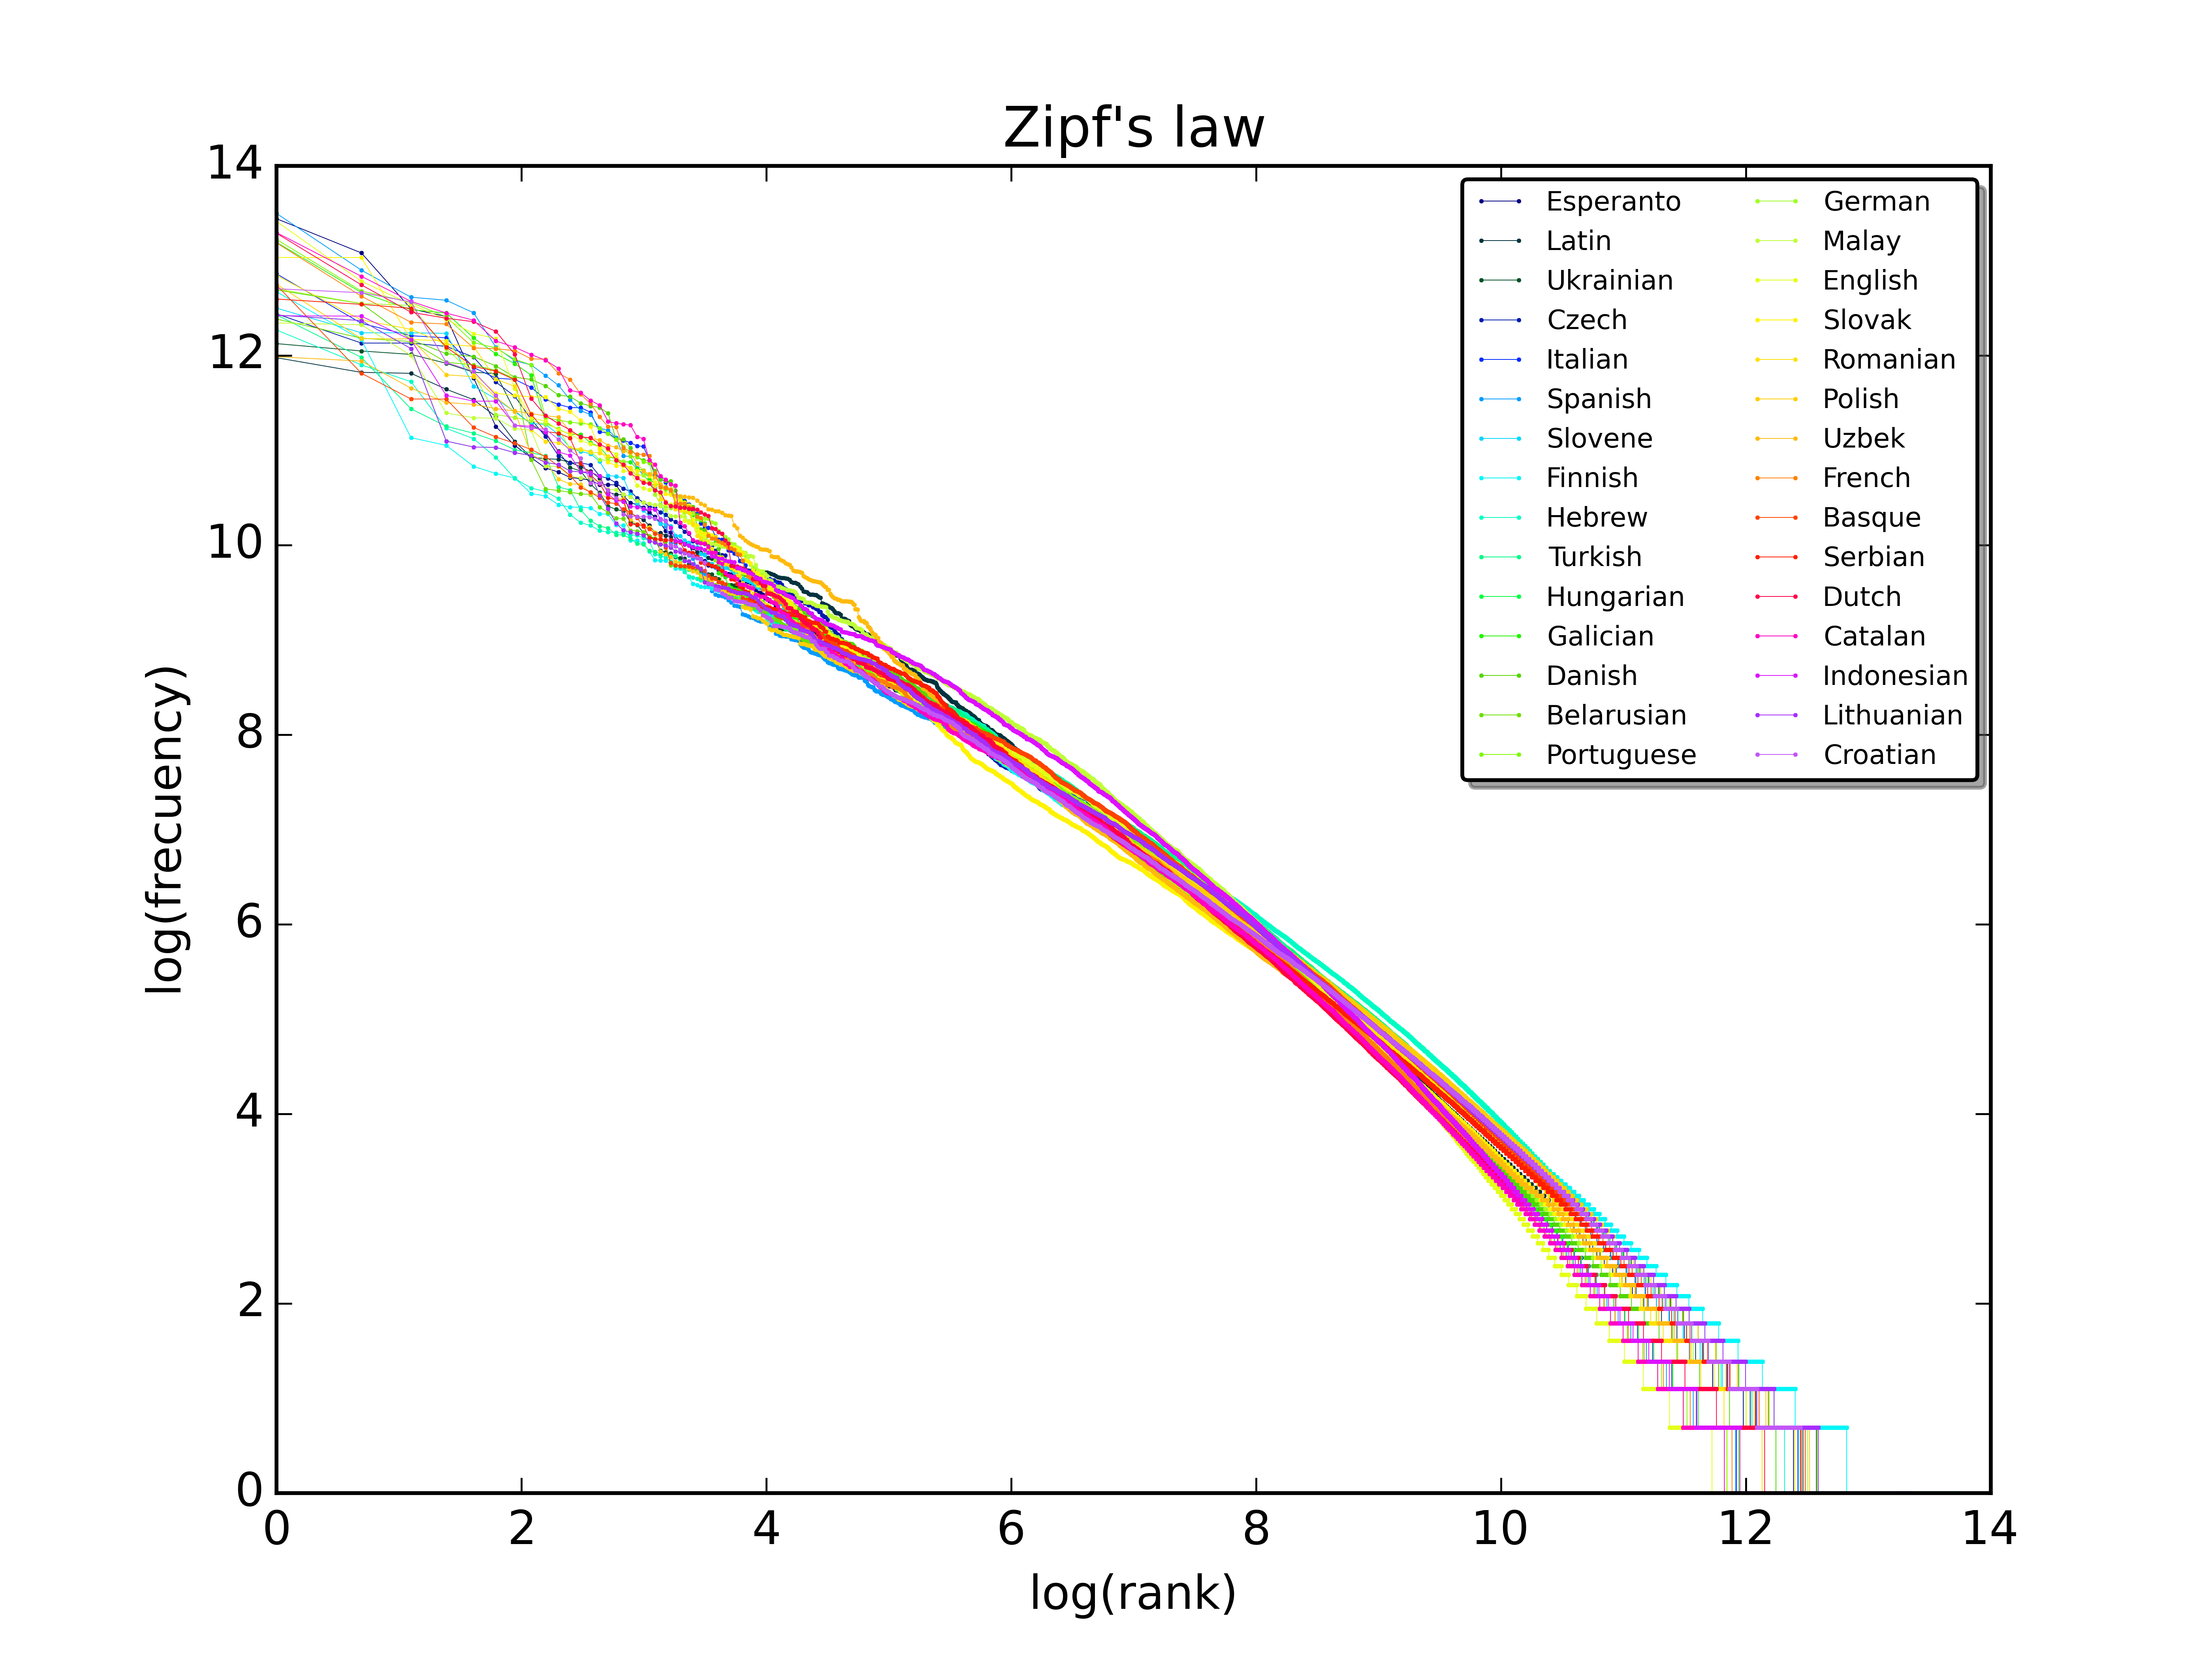
\includegraphics[width=\textwidth]{zipf_languages_wiki}
  \caption{
    The relationship of the logarithm of a word's frequency versus its rank for 30 human languages including Esperanto, an artifical language.
    Data from 30 Wikipedia dumps from October 2015.\\
    (Sergio Jimenez/Wikimedia, CC BY-SA 4.0 \cite{Jimenez2015a})}
  \label{fig:zipf_languages_wiki}
\end{figure}

This thesis focuses on a family of models \cite{Ferrer2007a} introduced initially to shed light into the origins of Zipf's law \cite{Ferrer2005a} \cite{Ferrer2003a}.
The focus of this thesis are two models from this family, which were generalized with the addition of a new parameter $\phi$. \cite{Ferrer2018a}
They are referred to as the ``\firstmodel{}'' and the ``\secondmodel{}'' throughout.
The key difference between these two models is whether they consider meanings to follow a probability distribution \emph{internal} or \emph{external} to the model.

It has been argued \cite{Ferrer2003a} \cite{Zipf1949a} that human language is result of attempting to minimize the effort of both the speaker and the hearer. Something that Zipf referred to as the \emph{principle of least effort}. These models follow this principle and are based on the minimization of a cost function, which is calculated in terms of information theoretic measures.

The motivation for this thesis is that these models could describe other language laws.
Zipf's law for word frequencies is quite well known but there are other patterns in human language.
One such pattern is the meaning-frequency law, also first reported by Zipf in his book. \cite{Zipf1949a}
Another is the relationship between the age of a word and its frequency, also studied by Zipf. \cite{Zipf1949a}
The consistent appearance of this law in 

In order to study these patterns in the model, a \CC{} program is implemented as part of this thesis.
This program is flexible and powerful enough to replicate previous results \cite{Ferrer2003a} \cite{Ferrer2005a} and also capable of generating results for newer versions of these models.
This program is one of the major contributions of this thesis.
It is released under an open source license with the hope that it can help others study these models and similar ones.

The rest of this chapter is divided as follows.
Section \ref{sec:introduction_background} revises the state of the art.
Previous articles about this family of models along with their responses and critiques, until the more current models are reached.
Section \ref{sec:introduction_general-goals} outlines the set of goals of this thesis without entering into detail about the models.
Section \ref{sec:introduction_model} introduces the family of models and the two models that are studied in detail.
Having introduced the model, section \ref{sec:introduction_goals} goes into more detail about the objectives of the thesis and section \ref{sec:introduction_hypothesis} covers the hypothesis.
Section \ref{sec:introduction_challenges} explains the main challenges that from this work.
Finally, Section \ref{sec:introduction_outline} outlines the rest of the thesis.

\section{Background}
\label{sec:introduction_background}

This section covers the ``state of the art'' or background of the thesis.
Section \ref{sec:introduction_background_linguistic-laws} explains some of the linguistic laws that have been found in more detail.
Section \ref{sec:introduction_background_similar} explores similar approximations to general problems and other models that have been proposed to explain Zipf's law, comparing them to these models.

\subsection{Linguistic laws}
\label{sec:introduction_background_linguistic-laws}

Here some space is dedicated to describe the linguistic laws that are studied in the model in more detail.

\subsubsection{Zipf's word-frequency law}

This law is well known as Zipf's law.
This thesis opens with its formulation in Equation \eqref{eq:zipf_law} due to its importance.
A word's frequency is inversely proportional to its rank when ordered by frequency.
The negative exponent $\alpha$ is typically around 1. \cite{Zipf1949a}

This is one of the most well known laws in quantitative linguistics and previous models were already seen to follow it \cite{Ferrer2003a} \cite{Ferrer2005a}.

\subsubsection{Zipf's meaning-frequency and meaning distribution laws}

Zipf's meaning-frequency law is less well known.
The law states the dependency between the number of meanings of a word $\mu$ and its frequency $f$, \cite{Zipf1949a}
\begin{equation*}
  \mu \propto f^\delta.
\end{equation*}
Zipf derived the meaning-frequency law from his famous law of word-frequency, Equation \eqref{eq:zipf_law} and from his law of meaning distribution,
\begin{equation*}
  \mu \propto i^{-\gamma}
\end{equation*}
where $i$ is the rank of the word and $\gamma \approx 1/2$

As with the constant $\alpha$, $\delta$ and $\gamma$ can be estimated using a regression method from data.

Zipf argued, and it has been proven \cite{Ferrer2016a} that
\begin{equation}
  \label{eq:relation-exponents}
  \delta = \frac{\gamma}{\alpha}.
\end{equation}

\subsubsection{Zipf's Age-frequency law}

Zipf argued in his book \cite{Zipf1949a} that older words (words that have existed in a language for a longer amount of time) would be more frequent.
This was tested empirically, as seen in Figure \ref{fig:zipf_word_ages}.

\begin{figure}
  \centering
  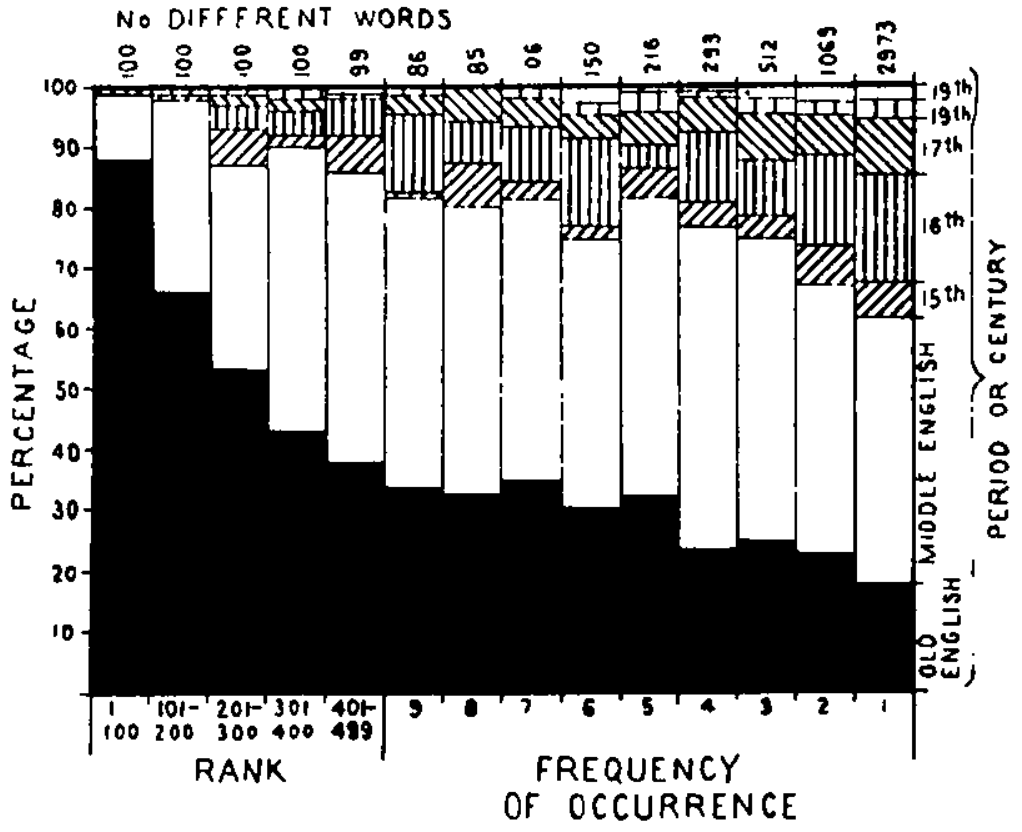
\includegraphics[width=\textwidth]{zipf_word_ages}
  \caption{
    Age of a word as a function of its frequency.
    The right side of the $y$ axis indicates the historical period or century when a word was introduced and the left side the percentage of words.
    Each of the colors and patterns of the columns in the graph correspond with a time period.
    As indicated in the $x$ axis, the first five columns refer to the most common words by rank, while the next columns refer to the words with the specified frequency of occurrence.
  }
  \label{fig:zipf_word_ages}
\end{figure}

\subsection{Similar research}
\label{sec:introduction_background_similar}

This section goes over other problems that have been solved similarly and other models that have attempted to explain Zipf's law.
A summary table between these alternative models and the models presented in this thesis is also shown.

\subsubsection{Similar approximations to general problems}

There has been research which can be related to the work done in this thesis.

Terry Regier argued \cite{Regier2007a} that color naming in human language corresponded with optimal partitions of the color space.
This is similar to the models presented here which, inspired by Zipf's \emph{principle of least effort}, consider language to be the result of optimizing speaker and hearer effort.
Regier's research showed that, indeed, color naming in many human languages was closely related to the optimal partitions of the color space.
The idea of language being ``optimal'' is not new.

In shortest path calculation algorithms, when a change takes place it is common to adjust the result based on the change instead of recalculating the entire process.
These changes offer speed ups of several orders of magnitude. \cite{Buriol2003a}
This is similar to the static vs dynamic approach (Section \ref{sec:introduction_model_dynamic-static}).
In this case, the dynamic algorithm offers a significant speedup that justifies issues such as the increase in mathematical complexity.

\subsubsection{Other models that explain Zipf's Law}

One of the most common explanations for Zipf's law is the random typing model.\cite{Miller1963a}
As a short summary, this model states that if characters are typed in sequence with a random chance of typing in a word separator then Zipf's law is reproduced.

While it is true that the Miller's random typing shows behavior similar to Zipf's law, it is also a shallow explanation that misses many important details.
To name a few issues, Miller's model assumes that words are independent from each other.
However, in human language, words are very much dependent on each other.
Random typing is often offered as a null hypothesis to the theory that Zipf's law comes from the \emph{principle of least effort}.
However, it has been shown \cite{Ferrer2020a} that random typing is an optimal coding process, which would make it not suitable as a null hypothesis either.

The random typing model would also not be able to explain other linguistic laws, such as the relationship between word age and frequency or the meaning distribution law, as it does not take into account the meanings nor the ages of words.
It could also not make more complex predictions, such as the vocabulary learning biases observed in children.

Another model which is used to explain the occurrences of power laws in nature is Simon's model.\cite{Simon1955}
This model argues that these power laws appear as a result of the way the system is formed.
In the case of language, constant addition of new words and addition of new instances of already existing words at a rate proportional to the number of instances of a word.

This model is not as widely known as the random typing model.
However, it is also not as powerful as the models presented in this thesis.
Like the random typing model, Simon's model cannot explain the meaning distribution law as it does not take meaning into account.
It also lacks the complexity to make predictions such as the vocabulary learning biases of children.
However, it could perhaps explain or at least try to predict the age frequency law, as the ages of words could be tracked.

Table \ref{tab:comparison_models} shows a comparison between the two models seen here (random typing and Simon's model) and the two models that this thesis presents.
The two models are further fleshed out in following sections.

\begin{table}
  \centering
  \begin{tabular}{p{2.5cm}p{1.5cm}p{1.5cm}p{1.5cm}p{1.5cm}p{1.5cm}p{1.5cm}}
    \toprule
                             & Random Typing & Simon's Model        & \Firstmodel{} ($\phi=0$) & \Secondmodel{} ($\phi=0$) & \Firstmodel{} ($\phi\neq 0$) & \Secondmodel{} ($\phi\neq 0$) \\
    \midrule
    Rank-frequency law       &      Yes      &      Yes             &             Yes          &           Yes             &           Yes            &           Yes             \\
    \addlinespace
    Meaning distribution law &      No       &      No              &             No           &           No              &           No             &           No              \\
    \addlinespace
    Age-frequency law        &      No       &    Unknown           &             Yes          &           Yes             &           Yes            &           Yes             \\
    \addlinespace
    Vocabulary learning bias &      No       &      No              &  Yes \cite{Ferrer2017a}  &         Unknown           &  Yes \cite{Carrera2021a} &         Unknown           \\
    \bottomrule
  \end{tabular}
  \caption{
    A summary table comparing various models of human language.
    Columns show various models of human language: Random Typing and Simon's model.
    Then the two models studied in this thesis: \firstm{} and \secondmodel{}.
    The value of $\phi$ indicates whether it is the older version of the model (equivalent of the general model with $\phi=0$) or the more general version with $\phi \neq 0$.
    Rows show various predictions that these models could or could not do.
    The vocabulary learning bias was shown to be predicted with the \firstmodel{} and more recently with the more generic version of the model ($\phi \neq 0$)
  }
  \label{tab:comparison_models}
\end{table}

\section{General goals}
\label{sec:introduction_general-goals}

Before introducing the models, this is a summary of the more general goals of this thesis.
Section \ref{sec:introduction_goals} offers a more specific set of goals within the context of the models now properly introduced.

The thesis aims to reproduce and verify the results of the previous models.
As the newer models are generic, they should also be able to reproduce the older models.
The new models should also be able to produce new results, which might be able to predict new linguistic laws that the older models could not.

Another goal is the creation of an open source program which can be used to test and replicate the results obtained.

\section{Introduction to the model}
\label{sec:introduction_model}

This is a short introduction to the models presented in this thesis.
In this section, mathematical definitions and notation common to both models is given.
They will be used throughout the remainder of the thesis and specially throughout Chapter \ref{cha:methods} where a full explanation of both models can be found.

Section \ref{sec:introduction_model_graph} presents the bipartite graphs that form the \emph{skeleton} of these models.
Section \ref{sec:introduction_model_info-theory} presents the information theoretic aspects, common to both models.
In Section \ref{sec:introduction_model_phi} the role of the $\phi$ parameter is explained.
Sections \ref{sec:introduction_model_first-model} and \ref{sec:introduction_model_second-model} cover the parts that unique to the \firstm{} and \secondmodel{} respectively. These are the \emph{flesh}, each covering the \emph{skeleton} in a different way.
Section \ref{sec:introduction_model_optimization} gives an overview of the optimization process.
Section \ref{sec:introduction_model_dynamic-static} explains the reasoning and difference of the static and dynamic versions of the implemented algorithms.

\subsection{Bipartite graph}
\label{sec:introduction_model_graph}

Both models studied in this thesis are based on the idea of a bipartite graph.
Bipartite graphs are comprised of two sets of elements and edges can only appear between an element of one set and an element of the other.

Our two sets are $S$ and $R$.
$S$ is a set of size $n$ containing all words.
The notation $s_i$ is used to refer to some element $i$ of the set $S$.
$R$ is a set of size $m$ containing all meanings.
The notation $r_j$ is used to refer to some element $j$ of the set $R$.

The bipartite graph is represented using the adjacency matrix $A_{n,m}$ (or simply $A$) in most cases.
$A_{n,m}$ is a \nbym{} binary matrix representing whether an edge exists or not in the graph.
Mathematically, each element of the matrix $A$ is defined as
\begin{equation*}
  %\label{eq:definition-aij}
  a_{i,j} =
  \begin{cases}
    1 & \text{if there exists an edge between $s_i \in S$ and $r_j \in R$} \\
    0 & \text{otherwise.}
  \end{cases}
\end{equation*}

In some cases it is more convenient to represent the bipartite graph as the set $E$ of all edges,
\begin{equation*}
  %\label{eq:definition-E}
  E = \Set{(s_i,r_j)}{\text{there exists an edge between $s_i \in S$ and $r_j \in R$}}.
\end{equation*}
For brevity, the pair $(s_i, r_j)$ is sometimes replaced by the simpler form $(i,j)$.

The degree of the word $i$ is given as $\mu_i$, while the degree of a meaning $j$ is given as $\omega_j$.

Figure \ref{fig:graph-example-base} displays an example of a simple bipartite graph.
A graphical representation is included, as well as the corresponding values of the mathematical concepts discussed in this section up to here.

\begin{figure}
  \centering
  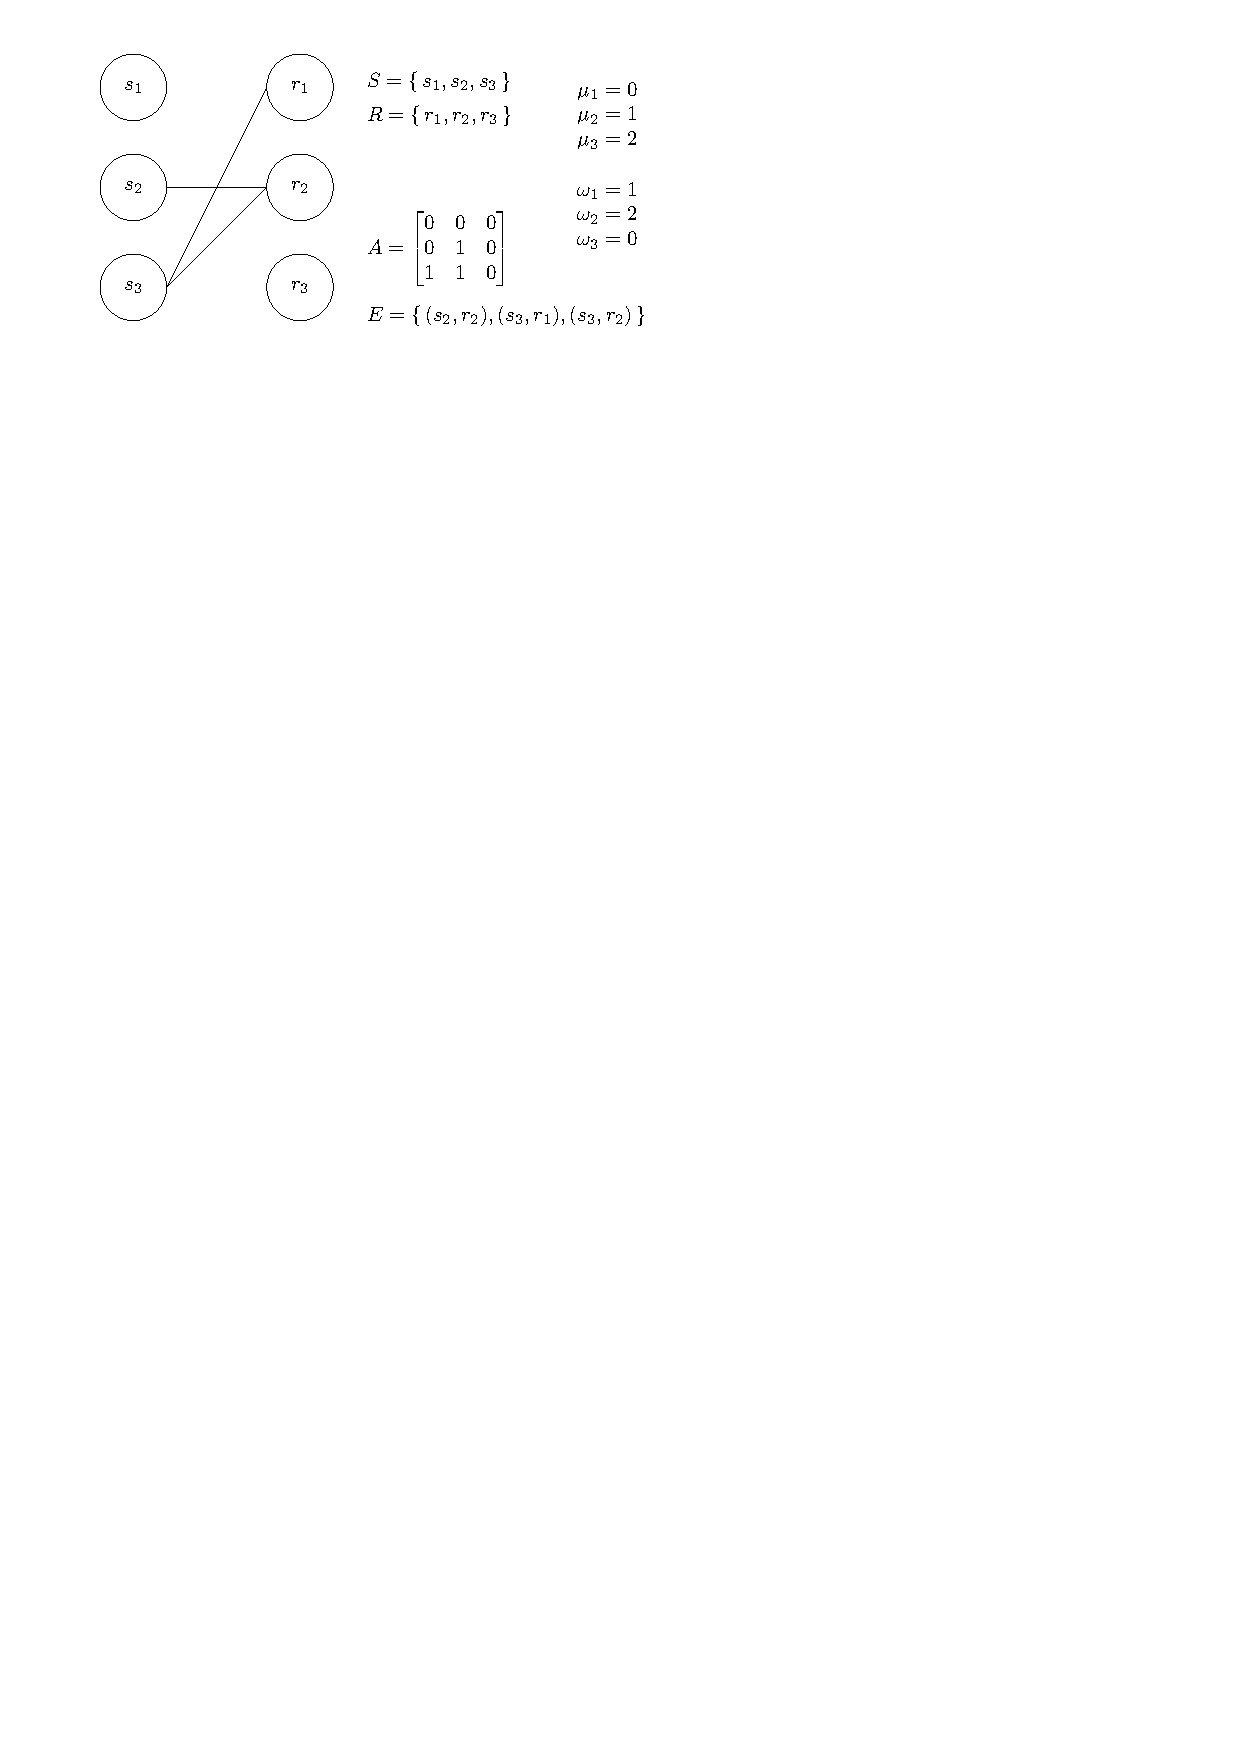
\includegraphics[width=\textwidth]{graph_example_base}
  \caption{%
    A bipartite graph with the corresponding adjacency matrix $A$, set of edges $E$ and vertex degrees $\mu$ and $\omega$ for each vertex.
  }
  \label{fig:graph-example-base}
\end{figure}

\subsection{Information theory}
\label{sec:introduction_model_info-theory}

Information theory measures are used to compute the cost function of the optimization process.
Here we go through a short overview of information theory formulas.

The general formula for the entropy of a set $X$ is
\begin{equation}
  \label{eq:definition-entropy-generic}
  H(X) = \sum_{x \in X} p(x) \log p(x)
\end{equation}
where $p(x)$ is the probability associated with the element $x$.
The general formula for the joint entropy of two sets $X$ and $Y$ is defined as
\begin{equation}
  \label{eq:definition-joint-entropy-generic}
  H(X,Y) = \sum_{x \in X} \sum_{y \in Y} p(x,y) \log p(x,y)
\end{equation}
where $p(x,y)$ is the joint probability of the elements $x$ and $y$.

Any other information theoretic measures concerning two sets can be obtained from $H(X)$, $H(Y)$ and $H(X,Y)$.
Mutual information
\begin{equation*}
  I(X,Y) = H(X) + H(Y) - H(X,Y),
\end{equation*}
and conditional entropies
\begin{equation*}
  H(X|Y) = H(X,Y) - H(X)
\end{equation*}
and
\begin{equation*}
  H(Y|X) = H(X,Y) - H(Y).
\end{equation*}
The diagram on Figure \ref{fig:relationships-entropies} shows these relationships in a more visual way.

\begin{figure}
  \centering
  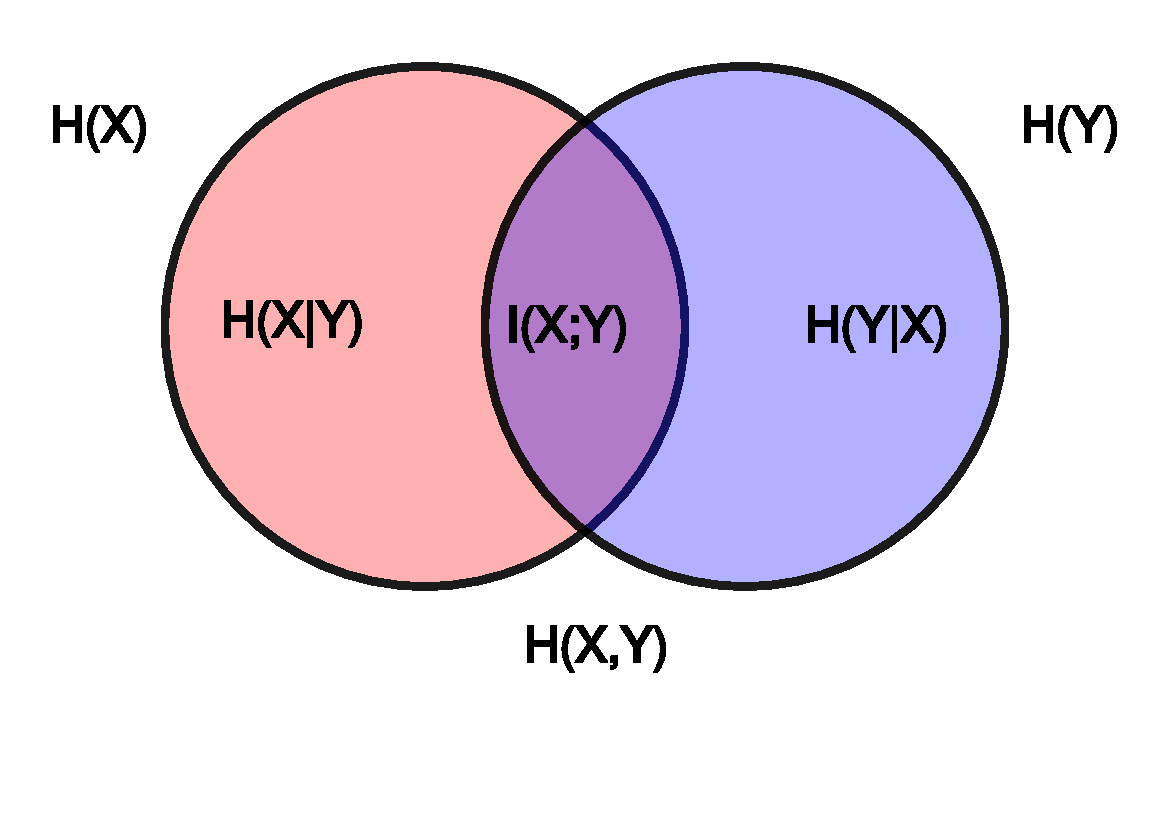
\includegraphics[width=\textwidth]{relationships_entropies}
  \caption{
    This diagram illustrates the relationships between information theoretic measures for two sets $X$ and $Y$.
    The area occupied by both left and right circle is the joint entropy $H(X,Y)$.
    The circle on the left (both the red and the violet areas) represents the marginal entropy $H(S)$ while the circle on the right (both blue and violet areas) represents the marginal entropy $H(Y)$.
    The red area is the conditional entropy $H(X|Y)$ while the blue area represents the conditional entropy $H(Y|X)$.
    The violet area represents the mutual information $I(X,Y)$.
  }
  \label{fig:relationships-entropies}
\end{figure}

Based on Equation \ref{eq:definition-entropy-generic}, we define the entropies of words and meanings, $H(S)$ and $H(R)$ respectively, as
\begin{equation}
  \label{eq:definition-HS}
  H(S) = \sum_{i=1}^n p(s_i) \log p(s_i)
\end{equation}
and
\begin{equation}
  \label{eq:definition-HR}
  H(R) = \sum_{j=1}^m p(r_j) \log p(r_j).
\end{equation}
We also define the joint entropy of words and meanings, from Equation \ref{eq:definition-joint-entropy-generic}, as
\begin{equation}
  \label{eq:definition-HSR}
  H(S,R) = \sum_{i=1}^n \sum_{j=1}^m p(s_i, r_j) \log p(s_i, r_j).
\end{equation}

\subsection{The $\phi$ parameter}
\label{sec:introduction_model_phi}

\redtxt{(we're making more general versions of previous model which now depend
  on more stuff but can be brought back to previous models by setting phi to
  0)}

The $\phi$ parameter, which has already appeared up to this point, is used to generalize the older versions of the two main models studied.

In \cite{Ferrer2005a} and \cite{Ferrer2003a} these two models were introduced.
Later, the $\phi$ parameter is added to generalize the model and hopefully be able to predict more linguistic laws \cite{Ferrer2018a}.

As is presented in the following sections, when $\phi=0$, the older models are retrieved from the newer ones.

\subsection{The \firstmodel{}}
\label{sec:introduction_model_first-model}

In this model, the joint probability of a word $s_i$ and a meaning $r_j$ is proportional to the product of their degrees to the $\phi$ power.
When $\phi=0$, the joint probability depends only on whether there is a connection between the word and the meaning.
Mathematically,
\begin{equation*}
  \label{eq:psirj-proportional-mui-wj}
  p(s_i, r_j) \propto a_{i,j} (\mu_i \omega_j)^\phi.
\end{equation*}
When $\phi=0$ we recover a previous simpler model \cite{Ferrer2005a}.

The actual joint probability is derived from Equation \ref{eq:psirj-proportional-mui-wj}, and from it the marginal probabilities of words and meanings are also derived.
Ultimately this leads to the information theoretic equations seen in Section \ref{sec:introduction_model_info-theory}.

\subsection{The \secondmodel{}}
\label{sec:introduction_model_second-model}

This model was introduced in \cite{Ferrer2003a} with meaning probabilities being constant and disconnected meanings being disallowed.
Here we present a generalization of the previous model.
In this model, the probability of a meaning $r_j$ is given \emph{a priori} as $\pi(r_j)$.
It is possible for a meaning to be disconnected from any words, in which case $p(r_j) = 0$.
In \cite{Ferrer2003a} disconnected meanings were disallowed and $\pi(r_j) = \frac{1}{m}$.
Additionally, $\phi=0$ in Equation \ref{eq:prop-cond-prob_second-model}.
Here $\pi(r_j)$ can follow any probability distribution and disconnected meanings are allowed.
Zero values of $\pi(r_j)$ are disallowed, however, as meanings that could never occur are not the target of communication.

We then define $p(r_j)$ as
\begin{equation}
  \label{eq:prj-proportional-pirj}
  p(r_j) \propto (1 - \delta_{\omega_j,0}) \pi(r_j)
\end{equation}
where $\delta_{a,b}$ is the Kronecker delta,
\begin{equation*}
  \delta_{a,b} = \begin{cases}
    0 & \text{if}~a \neq b \\
    1 & \text{if}~a = b.
  \end{cases}
\end{equation*}
The word probability is then defined as the conditional probability of choosing a word given that a meaning has been chosen,
\begin{equation}
  \label{eq:prop-cond-prob_second-model}
  p(s_i | r_j) \propto a_{i,j} \mu_i^\phi.
\end{equation}

With the marginal meaning probability and the conditional probability of a word given a meaning, the joint probability and marginal word probability can be calculated.
From this the information theoretic equations are be obtained.

\subsection{Optimization}
\label{sec:introduction_model_optimization}

As seen in previous sections and will be seen in Section \ref{sec:introduction_hypothesis}, our hypothesis is that the empirical laws observed in human language are the result of minimizing the effort of speaker and hearer.

This effort is defined in terms of information theoretic measures.
We choose two competing forces.
$H(S)$, the entropy of the words, and $I(S,R)$, the mutual information between words and meanings.
It is the goal of any communications system to maximize $I(S,R)$. The smaller $I(S,R)$, the greater the effort for the hearer.
The higher the entropy of words, however, they harder they are to access.
When $H(S)=0$, only a single word has probability 1 while all others are 0, meaning that knowing which word to choose is trivial, while $H(S)$ is maximum when all words have equal probability, giving no indication of which should be chosen.

We define $\Omega(\lambda)$ as the cost function we aim to minimize,
\begin{equation}
  \label{eq:definition-Omega}
  \Omega(\lambda) = -\lambda I(S,R) + (1 - \lambda) H(S)
\end{equation}
where $0 \leq \lambda \leq 1$ is used to indicate the weight given to each of the two forces.
When $\lambda=0$, the minimization of $H(S)$ is completely favored while when $\lambda=1$ the maximization of $I(S,R)$ is.
When $\lambda=1/2$, they are equally favored.

The optimization process follows a Markov chain Monte Carlo method at zero temperature.
It consists of making mutations to $A$, chancing $a_{i,j}$ from 1 to 0 or from 0 to 1.
If a set of mutations results in a decrease of $\Omega$, they are kept.
Otherwise they are undone and another set is attempted.

\subsection{Dynamic and static equations}
\label{sec:introduction_model_dynamic-static}

As is seen later on, in Chapter \ref{cha:model}, two sets of equations are derived for the information theoretic equations necessary to calculate $\Omega$ (Equation \ref{eq:definition-Omega}).

A set of static equations recalculate everything from scratch.
The set of dynamic equations calculate the changes done only after a mutation to $A$ takes place.

As seen in Section \ref{sec:introduction_background_similar} this dynamic recalculation can be more efficient.
In the case of this thesis, small changes are continuously done to the graph, making several mutations to $A$ then reevaluating $\Omega$.
Dynamically accounting for the differences brought about for these changes is much more efficient than recalculating every single measure each time.

Dynamic calculation, however, brings its own set of problems, such as the increase in mathematical complexity and the introduction of greater floating point error.
Section \ref{sec:introduction_challenges_dynamic} goes over this in more detail while Section \ref{sec:methods_model-implementation} covers the measures taken in order to deal with these problems.

\section{Goals}
\label{sec:introduction_goals}

With the model introduced, more specific goals are stated. See also the overall goals in section \ref{sec:introduction_general-goals}.

\begin{itemize}
\item
  To create an open source tool implementing the general models.
  \begin{itemize}
  \item
    This tool should be both powerful and flexible, allowing to replicate previous results for the case $\phi=0$.
  \item
    It should also be efficient and fast enough that results with relatively large graphs can be obtained in a reasonable time. This means using dynamic equations.
  \item
    It should be relatively easy to use such that anyone who wishes to test these models by themselves can do it.
  \end{itemize}
\item
  Find out whether local minima exist.
  It is not clear whether there exists local minima for the case $\phi \neq 0$.
  The previous models where $\phi = 0$ have been analyzed mathematically \cite{Salge2015} \cite{Prokopenko2010}.
  The case $\phi \neq 0$ is more complex and would be very hard to analyze mathematically to this level.
  It is possible that the optimization stops at a point where the function could still be minimized further but it is hard to find the set of mutations that minimize it.
  Or it could be that the function does reach a local minima.
\end{itemize}

\section{Hypothesis}
\label{sec:introduction_hypothesis}

Several hypothesis are stated here.

As seen in section \ref{sec:introduction_background} and in \cite{Ferrer2018a}, there is a relationship between the exponents of the Zipf's word-frequency and meaning-frequency laws.
See Equation \ref{eq:relation-exponents}.
The main hypothesis of the thesis is that linguistic laws appear due to an optimization process.
It is under this assumption that the entire model works and the results are obtained.
In the model we also neglect any effects of social interaction, which are the basis of other approaches to investigating human language such as the naming game \cite{Baronchelli2006}.
Another hypothesis is that the optimization process does not necessarily arrive at a local minimum.

\section{Challenges}
\label{sec:introduction_challenges}

The main challenges presented by this thesis are outlined here.
They are divided into three categories: challenges relating to quantitative linguistics in Section \ref{sec:introduction_challenges_quant-lin}, computational challenges in Section \ref{sec:introduction_challenges_computational} and the challenges brought by the use of a dynamic calculation technique, in section \ref{sec:introduction_challenges_dynamic}.

\subsection{Quantitative linguistics}
\label{sec:introduction_challenges_quant-lin}

The challenges relating to quantitative linguistics come from the fact that current models already can make some predictions.
Can these new models predict anything new? Can they still make the predictions that the old models already could?
Specifically, the $\phi=0$ models presented in \cite{Ferrer2005a} and \cite{Ferrer2003a} already showed the appearance of Zipf's law of word frequencies.
Can the new models with $\phi \neq 1$ (and more specifically $\phi=1$) make any new predictions such as the law of meaning frequency, or the one relating word ages and frequencies?
Can they still predict Zipf's law?

\subsection{Computational}
\label{sec:introduction_challenges_computational}

The computational challenges relate to the implementation of the model.

Verification is a very important step.
The mathematics are complex, specially in the dynamic case, and a single mistake can invalidate all the results.
Therefore, the implementation must be verified thoroughly and completely.

The stop condition of the optimization process is also difficult to properly implement.
The algorithm should stop once it can be reasonably sure that a minimum has been reached.
However, due to the size search space, it is unfeasible to check every possible set of mutations.

An important challenge is recalculating $\Omega$ efficiently enough that results with relatively big $n$ and $m$ can be executed in a reasonable time.
The calculation of $\Omega$ directly influences the runtime of the program.
In order to speed it up, dynamic calculations are used.
Dynamic calculation, however, presents its own set of challenges.

\subsection{Dynamic calculation}
\label{sec:introduction_challenges_dynamic}

Dynamic calculation is much more mathematically complex than static calculation.
This complexity makes the likelihood of a bug being introduced much more likely.
Therefore the verification process must be even more thorough.

In addition to complexity, dynamic calculation implies many addition and subtraction operations.
These operations introduce greater floating point error than others (such as multiplication and division).
If the floating point error accumulates, it can change the result into a different one from the static method.
Dynamic and static approaches should lead to identical results.

\section{Outline of the thesis}
\label{sec:introduction_outline}

The rest of the thesis is organized as follows:

Chapter \ref{cha:model} gives more detail of the models, and all the mathematical detail concerning the models (although long derivations or simple proofs that are otherwise unrelated are left for Appendix \ref{cha:app_formulae}).
It is during this chapter that all the mathematics that are eventually implemented into the open source tool are showcased.
The computational aspects are also seen here, showing the computational complexity of implementing these formulas.
This chapter starts from the initial concepts seen in Section \ref{sec:introduction_model}.

Chapter \ref{cha:methods} goes into the implementation of the model.
It includes full descriptions of various implementation details, of the optimization algorithm, the decisions regarding parallelization of the code and the approach to verification.
It also covers some challenges unique to the implementation of the model and how they were resolved.

Chapter \ref{cha:results} introduces the results obtained from the open source tool.
It includes the figures from the previous models \cite{Ferrer2005a} and \cite{Ferrer2003a} implemented with $\phi=0$.
It also includes new data obtained by setting $\phi=1$.

Finally, Chapter \ref{cha:discussion} discusses the obtained results and their relation to certain linguistic laws that have been seen in this introduction.
Future work is also discussed in this chapter, including alternative optimization methods.

%%% Local Variables:
%%% mode: latex
%%% TeX-master: "tfm"
%%% End:

\chapter{Model}
\label{cha:model}

This chapter covers the details about the two models previously introduced in Chapter \ref{cha:introduction}, where a high level introduction to both the \firstmodel{} and the \secondmodel{} was given.
It follows a top down approach.
General concepts from both types of model are outlined first and the specific details from each model are given afterwards.

As a reminder of the previous chapter a very brief definition of the two models follows.
Both models are quite similar, they represent a way to connect words with meanings.
Both meanings and words are given probabilities of being used, from which information theoretic measures are derived, which are ultimately used to obtain a cost function.
The high level differentiating trait is the way in which the probability of a meaning is obtained.
In the first studied model (\firstmodel{}), the probabilities of both words and meanings are proportional to the number of connections.
In the second model (\secondmodel{}), the probabilities of meanings come from a distribution of \emph{a priori} probabilities.

The remainder of this chapter is divided into two sections.
Section \ref{sec:model_math} deals with the mathematical definitions of the models and it is more theoretical in nature.
Section \ref{sec:model_compute} outlines the computational aspects of the two models and it is more practical and implementation oriented.
This chapter does not deal with any actual details of the implementation of the model.
These details can be found in Chapter \ref{cha:methods}.

Note that Chapter \ref{cha:introduction} offers a high level revision of the graph theory and information theory concepts that will appear during the rest of this chapter.

\section{Mathematical aspect}
\label{sec:model_math}

This section covers the mathematical definition of the model.
Section \ref{sec:model_math_graph} introduces concepts common to both models.
These concepts are then extended for either the \firstmodel{} or the \secondmodel{} in Sections \ref{sec:model_math_first-model} and \ref{sec:model_math_second-model} respectively.

\subsection{Common concepts}
\label{sec:model_math_graph}

In this section, mathematical definitions and notation common to both models is given.
They will be used throughout the remainder of the thesis.

Both models studied in this thesis are based on the idea of a bipartite graph $G_{n,m}$.
Bipartite graphs are comprised of two sets of elements and edges can only appear between an element of one set and an element of the other.

Our two sets are $S$ and $R$.
$S$ is a set of size $n$ containing all words.
The notation $s_i$ is used to refer to some element $i$ of the set $S$.
$R$ is a set of size $m$ containing all meanings.
The notation $r_j$ is used to refer to some element $j$ of the set $R$.

The bipartite graph is represented using the adjacency matrix $A_{n,m}$ (or simply $A$) in most cases.
$A_{n,m}$ is a \nbym{} binary matrix representing whether an edge exists or not in the graph.
Mathematically, each element of the matrix $A$ is defined as
\begin{equation*}
  %\label{eq:definition-aij}
  a_{i,j} =
  \begin{cases}
    1 & \text{if there exists an edge between $s_i \in S$ and $r_j \in R$} \\
    0 & \text{otherwise.}
  \end{cases}
\end{equation*}

In some cases it is more convenient to represent the bipartite graph as the set $E$ of all edges,
\begin{equation*}
  %\label{eq:definition-E}
  E = \Set{(s_i,r_j)}{\text{there exists an edge between $s_i \in S$ and $r_j \in R$}}.
\end{equation*}
For brevity, the tuple $(s_i, r_j)$ is sometimes replaced by the simpler form $(i,j)$.

A notation is defined for the degree of the vertices in the graph.
The word $s_i$ has degree $\mu_i$, while the meaning $r_j$ has degree $\omega_j$.
Mathematically, $\mu$ and $\omega$ are defined
\begin{equation}
  \label{eq:definition-mu}
  \mu_i = \sum_{j=1}^m a_{i,j}
\end{equation}
and
\begin{equation}
  \label{eq:definition-omega}
  \omega_j = \sum_{i=1}^n a_{i,j}.
\end{equation}

There is an additional parameter of the models, $\phi$, which is not directly related to the bipartite graph.
This parameter appears in both models and it is used to ``emphasize'' the effect of the vertex degrees in the calculations.
As explained in previous sections, this parameter is a new addition to the models originally presented in \cite{Ferrer2005a} and \cite{Ferrer2003a}.

Figure \ref{fig:graph-example-base} displays an example of a simple $G_{3,3}$ graph.
A graphical representation is included, as well as the corresponding values of the mathematical concepts discussed in this section up to here.

\begin{figure}
  \centering
  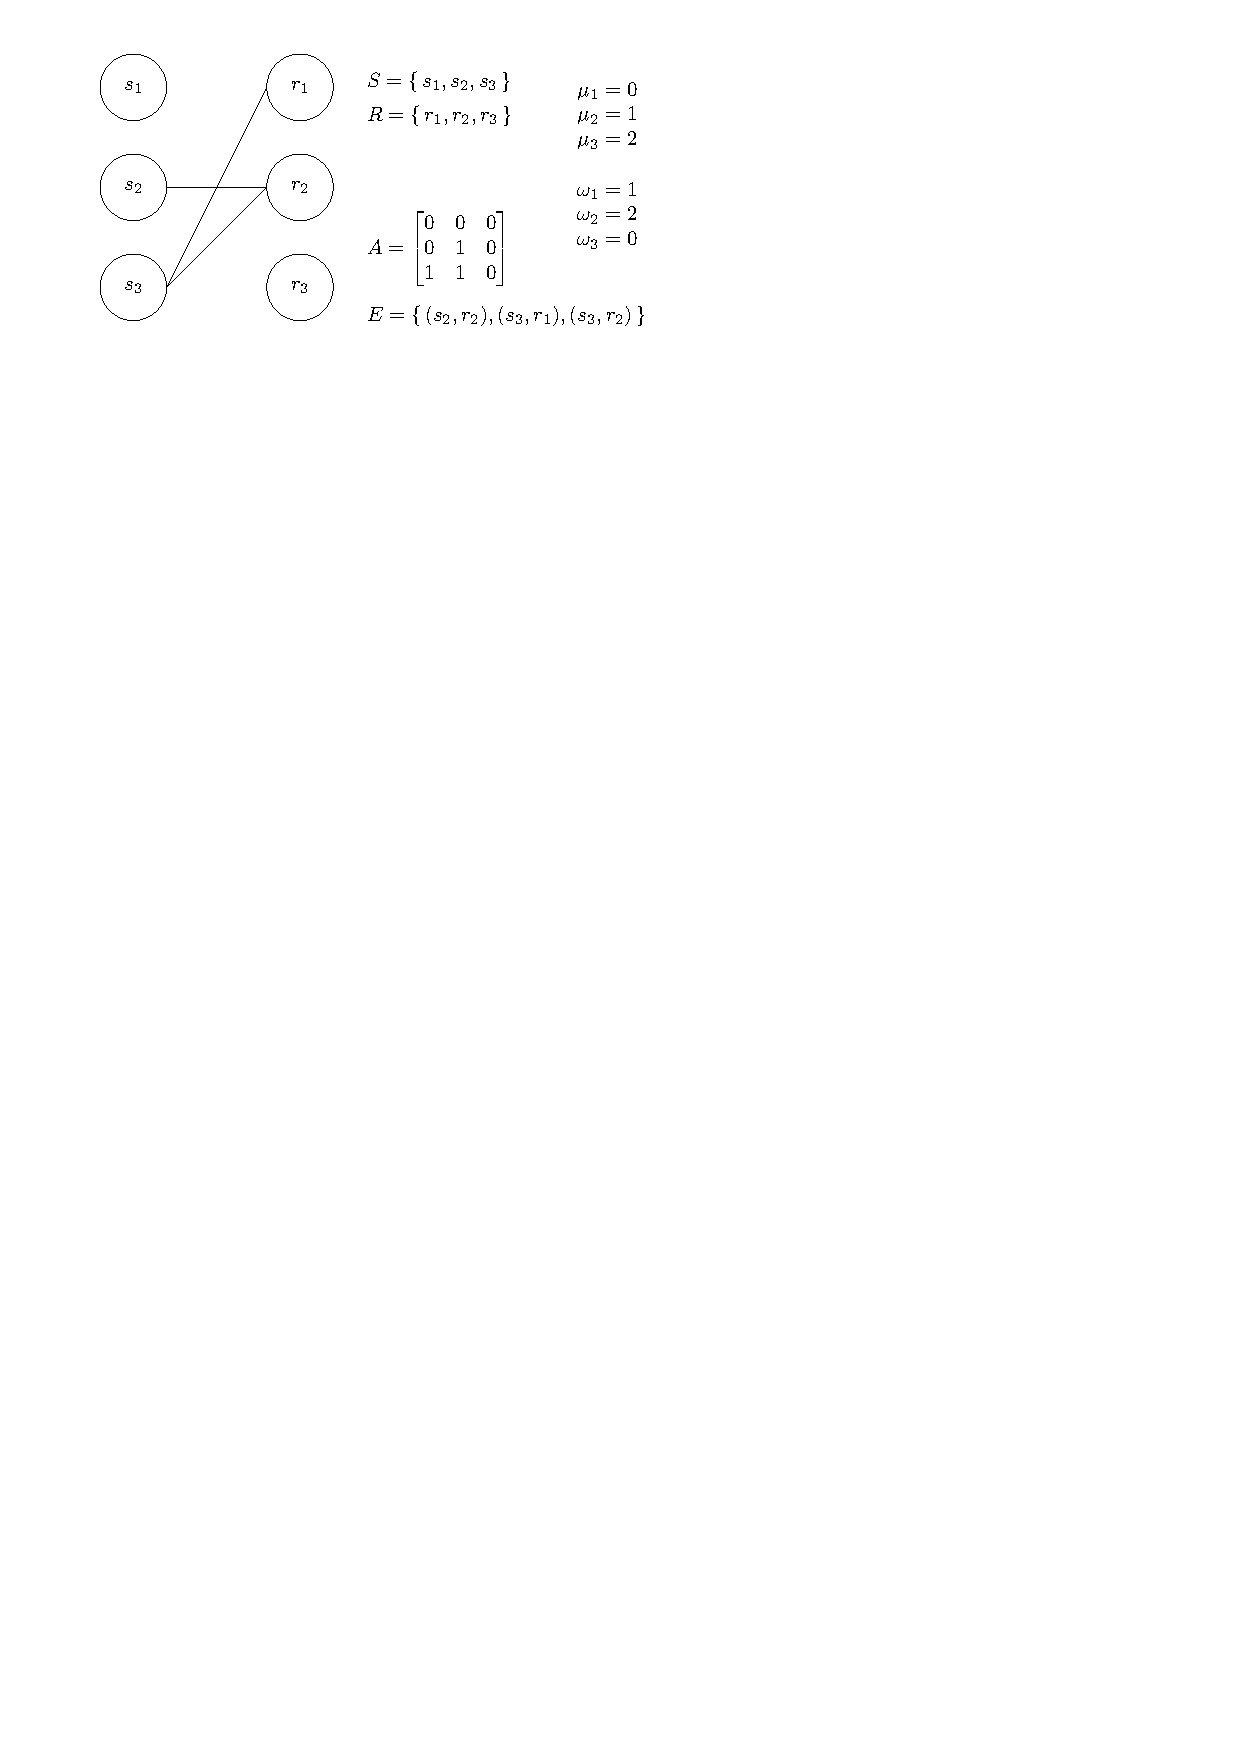
\includegraphics[width=\textwidth]{graph_example_base}
  \caption{%
    A $G_{3,3}$ bipartite graph with the corresponding adjacency matrix $A$, set of edges $E$ and vertex degrees $\mu$ and $\omega$ for each vertex.
  }
  \label{fig:graph-example-base}
\end{figure}

With the parameter $\phi$, the definitions of $\mu$ and $\omega$ can be generalized.
$\mu_\phi$ and $\omega_\phi$ are defined as
\begin{equation}
  \label{eq:definition-muphi}
  \mu_{\phi,i} = \sum_{j=1}^m a_{i,j} \omega_j^\phi
\end{equation}
and
\begin{equation}
  \label{eq:definition-omegaphi}
  \omega_{\phi,i} = \sum_{i=1}^n a_{i,j} \mu_i^\phi.
\end{equation}
It can be seen that when $\phi=0$ Equation \eqref{eq:definition-muphi} becomes Equation \eqref{eq:definition-mu} and Equation \eqref{eq:definition-omegaphi} becomes Equation \eqref{eq:definition-omega}.
In other words, $\mu_{0,i} = \mu_i$ and $\omega_{0,j} = \omega_j$

\subsection{The \firstmodel{}}
\label{sec:model_math_first-model}

This model is defined by the joint probability of a word $s_i$ and a meaning $r_j$.
This probability must be proportional to the product of the degrees of $s_i$ and $r_j$ and it must be zero if there is no edge between $s_i$ and $r_j$.
Mathematically,
\begin{equation*}
  %\label{eq:psirj-proportional-mui-wj}
  p(s_i, r_j) \propto a_{i,j} (\mu_i \omega_j)^\phi,
\end{equation*}
where the parameter $\phi$ is used to control the effect of the vertex degrees.
As previously noted, the original model from \cite{Ferrer2005a} is equivalent to this one but with $\phi=0$ and so, the vertex degrees have no effect in the joint probability. \redtxt{no ho tinc gaire clar... desde on ``comencen'' les equacions del primer model?}

From this definition, equations for the marginal probabilities are derived, which in turn are used to obtain the information theory expressions in the cost function $\Omega$ (Equation \eqref{eq:definition-Omega}).
From these expressions, dynamic equations are derived to obtain the change experienced by the entropies after a single mutation has occurred on the adjacency matrix $A$.

\subsubsection{Joint Probability}

Adding a normalizing factor $M_\phi$, the joint probability becomes
\begin{equation}
  \label{eq:definition-psirj_first-model}
  p(s_i, r_j) = \frac{1}{M_\phi} a_{i,j} (\mu_i \omega_j)^\phi.
\end{equation}

This normalizing factor is obtained by applying the definition of probability
\begin{equation*}
  \sum_{i=1}^n \sum_{j=1}^m p(s_i, r_j) = 1.
\end{equation*}
Then,
\begin{equation*}
  M_\phi = \sum_{i=1}^n \sum_{j=1}^m a_{i,j} (\mu_i \omega_j)^\phi
\end{equation*}
or equivalently
\begin{equation}
  \label{eq:definition-Mphi}
  M_\phi = \sum_{(i,j) \in E}^n (\mu_i \omega_j)^\phi.
\end{equation}

\subsubsection{Marginal Probabilities}

Formulas for the marginal probabilities $p(s_i)$ and $p(r_j)$ are derived from the joint probability using the general formula
\begin{equation}
  \label{eq:marginal-from-joint}
  p(x) = \sum_{y \in Y} p(x,y).
\end{equation}
Applying Equation \eqref{eq:marginal-from-joint},
\begin{equation*}
  p(s_i) = \frac{\mu_i^\phi}{M_\phi} \sum_{j=1}^m a_{i,j} \omega_j^\phi.
\end{equation*}
Recall Equation \eqref{eq:definition-muphi},
\begin{equation}
  \label{eq:definition-psi_first-model}
  p(s_i) = \frac{\mu_i^\phi \mu_{\phi,i}}{M_\phi}.
\end{equation}
Symmetrically applying Equation \eqref{eq:marginal-from-joint} to obtain $p(r_j)$ and applying Equation \eqref{eq:definition-omegaphi} instead we obtain
\begin{equation}
  \label{eq:definition-prj_first-model}
  p(r_j) = \frac{\omega_j^\phi \omega_{\phi,j}}{M_\phi}.
\end{equation}

\subsubsection{Entropies}

$H(S,R)$ is obtained by applying the joint probability found in Equation \eqref{eq:definition-psirj_first-model} to Equation \eqref{eq:definition-HSR},
\begin{equation}
  \label{eq:step-HSR}
  H(S,R) = -\sum_{i=1}^n \sum_{j=1}^m \frac{1}{M_\phi} a_{i,j} (\mu_i \omega_j)^\phi \log \left( a_{i,j} (\mu_i \omega_j)^\phi \right).
\end{equation}

This expression can be refined taking advantage of the equality
\begin{equation}
  \label{eq:definition-trick}
  -\sum_i \frac{x_i}{T} \log\frac{x_i}{T} = \log T - \frac{1}{T} \sum_i x_i \log x_i
\end{equation}
which holds as long as
\begin{equation*}
  T = \sum_i x_i.
\end{equation*}
The full derivation of Equation \eqref{eq:definition-trick} can be found in Appendix \ref{sec:app_formulae_trick}.

Applying Equation \eqref{eq:definition-trick} to Equation \eqref{eq:step-HSR} we obtain
\begin{equation*}
  H(S,R) = \log M_\phi - \frac{\phi}{M_\phi} \sum_{i=1}^n \sum_{j=1}^m a_{i,j} \left( (\mu_i \omega_j)^\phi \log a_{i,j} \mu_i \omega_j \right)
\end{equation*}
using $E$ in the summation and adopting the convention that $0 \log 0 = 0$
\begin{equation}
  \label{eq:definition-HSR_first-model}
  H(S,R) = \log M_\phi - \frac{\phi}{M_\phi} \sum_{(i,j) \in E} (\mu_i \omega_j)^\phi \log \mu_i \omega_j
\end{equation}
is reached.

The marginal word entropy is found applying the marginal probability in Equation \eqref{eq:definition-psi_first-model} to the definition of $H(S)$ in Equation \eqref{eq:definition-HS}
\begin{equation*}
  H(S) = -\sum_{i=1}^n \frac{\mu_i \mu_{\phi,i}}{M_\phi} \log \frac{\mu_i \mu_{\phi,i}}{M_\phi}.
\end{equation*}
Equation \eqref{eq:definition-trick} can be applied immediately, obtaining
\begin{equation}
  \label{eq:definition-HS_first-model}
  H(S) = \log M_\phi - \frac{1}{M_\phi} \sum_{i=1}^n \mu_i^\phi \mu_{\phi,i} \log \mu_i^\phi \mu_{\phi,i}.
\end{equation}
The convention $0 \log 0 = 0$ is applied here for disconnected words (where $\mu_i = 0$).

The marginal meaning entropy is found symmetrically, the marginal probability (Equation \eqref{eq:definition-prj_first-model}) is applied to the definition of $H(R)$ (Equation \eqref{eq:definition-HR}).
With Equation \eqref{eq:definition-trick}, we obtain
\begin{equation}
  \label{eq:definition-HR_first-model}
  H(R) = \log M_\phi - \frac{1}{M_\phi} \sum_{j=1}^m \omega_j^\phi \omega_{\phi,j} \log \omega_j^\phi \omega_{\phi,j}.
\end{equation}
also using the convention $0 \log 0 = 0$ for disconnected meanings ($\omega_j=0$).

\subsubsection{Dynamic Equations}

The full derivation of the dynamic equations can be found in \cite{Carrera2021a}.
Here only the final expressions of the dynamic equations are given.

Starting with compact expressions of the entropies (Equations \eqref{eq:definition-HSR_first-model}, \eqref{eq:definition-HS_first-model} and \eqref{eq:definition-HR_first-model})
\begin{align}
  \label{eq:definition-HSR_first-model_compact}
  H(S,R) &= \log M_\phi - \frac{\phi}{M_\phi} X(S,R) \\
  \label{eq:definition-HS_first-model_compact}
  H(S) &= \log M_\phi - \frac{1}{M_\phi} X(S) \\
  \label{eq:definition-HR_first-model_compact}
  H(R) &= \log M_\phi - \frac{1}{M_\phi} X(R)
\end{align}
with
\begin{align}
  \label{eq:definition-XSR_first-model_dynamic}
  X(S,R) &= \sum_{(i,j) \in E} x(s_i, r_j) \\
  \label{eq:definition-XS_first-model_dynamic}
  X(S) &= \sum_{i=1}^n x(s_i) \\
  \label{eq:definition-XR_first-model_dynamic}
  X(R) &= \sum_{j=1}^m x(r_j) \\
  \label{eq:definition-Xsirj_first-model_dynamic}
  x(s_i, r_J) &= (\mu_i\omega_j)^\phi \log \mu_i\omega_j \\
  \label{eq:definition-Xsi_first-model_dynamic}
  x(s_i) &= \mu_i^\phi \mu_{\phi,i} \log \mu_i^\phi \mu_{\phi,i} \\
  \label{eq:definition-Xrj_first-model_dynamic}
  x(r_j) &= \omega_j^\phi \omega_{\phi,j} \log \omega_j^\phi \omega_{\phi,j}.
\end{align}

A prime mark is used to indicate a new value of a certain variable after a mutation has taken place.
A variable without a prime mark indicates the value before the mutation took place.
Suppose that $a_{i,j}$ mutates.
Then
\begin{align}
  \label{eq:definition-aij_dynamic}
  a'_{i,j} &= 1 - a_{i,j} \\
  \label{eq:definition-mui_dynamic}
  \mu'_i &= \mu_i + (-1)^{a_{i,j}} \\
  \label{eq:definition-wj_dynamic}
  \omega'_j &= \omega_j + (-1)^{a_{i,j}}
\end{align}

We define the set of neighbors of any word $s_i$
\begin{equation}
  \label{eq:definition-Gamma-S}
  \Gamma_S(i) = \Set{r_j}{(s_i,r_j) \in E},
\end{equation}
and similarly the set of neighbors of any meaning $r_j$
\begin{equation}
  \label{eq:definition-Gamma-R}
  \Gamma_R(j) = \Set{s_i}{(s_i,r_j) \in E}.
\end{equation}

Then, for any $k$ such that $1 \leq k \leq n$, we have that
\begin{equation}
  \label{eq:definition-muphik_dynamic}
  \mu'_{\phi,k} = \begin{cases}
    \mu_{\phi,k} - a_{ij} \omega_j^\phi + (1 - a_{ij}) {\omega_j'}^\phi & \text{if}~k=i \\
    \mu_{\phi,k} - \omega_j^\phi + {\omega_j'}^\phi & \text{if}~k \in \Gamma_R(j)~\text{and}~k \neq i \\
    \mu_{\phi,k} & \text{otherwise}.
  \end{cases}
\end{equation}
Likewise, for any $l$ such that $1 \leq l \leq m$, we have that
\begin{equation}
  \label{eq:definition-wphik_dynamic}
  \omega'_{\phi,l} = \begin{cases}
    \omega_{\phi,l} - a_{ij} \mu_i^\phi + (1 - a_{ij}) {\mu_i'}^\phi & \text{if}~l=j \\
    \omega_{\phi,l} - \mu_i^\phi + {\mu_i'}^\phi & \text{if}~l \in \Gamma_S(i)~\text{and}~l \neq j \\
    \omega_{\phi,l} & \text{otherwise}.
  \end{cases}.
\end{equation}
These variables can be applied to Equations \eqref{eq:definition-Xsirj_first-model_dynamic}, \eqref{eq:definition-Xsi_first-model_dynamic} and \eqref{eq:definition-Xrj_first-model_dynamic} directly to obtain their values.

We define the set $N_{i,j}$ \redtxt{(originalment $E(i,j)$ però ja es fa servir $E$ com el conjunt d'arestes del graf)} as the set of all edges connecting$s_i$ and $r_j$ with their neighbors.
That is,
\begin{equation}
  \label{eq:definition-Nij}
  N_{i,j} = \Set{(i,l)}{l \in \Gamma_S(i)} \cup \Set{(k,j)}{k \in \Gamma_R(j)}
\end{equation}

With these definitions, we can now obtain the expressions of $X'(S,R)$ from $X(S,R)$ and of $M'_\phi$ from $M_\phi$.
\begin{equation*}
\begin{split}
  M'_{\phi} = M_\phi &- \left[ \sum_{(k,l) \in N_{i,j}}(\mu_k \omega_l)^\phi \right]   - a_{ij} (\mu_i \omega_j)^\phi \\
                     &+ \left[ \sum_{(k,l) \in N_{i,j}}(\mu'_k \omega'_l)^\phi \right] + (1 - a_{ij}) (\mu'_i \omega'_j)^\phi.
\end{split}
\end{equation*}
Similarly, the new value of $X(S,R)$ will be
\begin{equation}
  \label{eq:definition-XSR_first-model_dynamic}
\begin{split}
  X'(S,R) = X(S,R) &- \left[ \sum_{(k,l) \in N_{i,j}}x(s_k, r_l) \right] - a_{ij} x(s_i, r_j) \\
                   &+ \left[ \sum_{(k,l) \in N_{i,j}}x'(s_k, r_l)\right] + (1 - a_{ij}) x'(s_i, r_j).
\end{split}
\end{equation}

The expressions of $X'(S)$ from $X(S)$ and $X'(R)$ from $X(R)$ used to dynamically update Equations \eqref{eq:definition-XSR_first-model_dynamic}, \eqref{eq:definition-XS_first-model_dynamic} and \eqref{eq:definition-XR_first-model_dynamic} are
\begin{equation}
  \label{eq:definition-XS_first-model_dynamic}
  X'(S) = X(S) - \left[ \sum_{k \in \Gamma_{R}(j)} x(s_k) \right] - a_{ij} x(s_i) + \left[ \sum_{k \in \Gamma_{R}(j)} x'(s_k) \right] + (1 - a_{ij}) x'(s_i)
\end{equation}
and
\begin{equation}
  \label{eq:definition-XR_first-model_dynamic}
  X'(R) = X(R) - \left[ \sum_{l \in \Gamma_{S}(i)} x(r_l) \right] - a_{ij} x(r_j) + \left[ \sum_{l \in \Gamma_{S}(i)} x'(r_l) \right] + (1 - a_{ij}) x'(r_j).
\end{equation}

Again, the full derivation of these equations can be found in \cite{Carrera2021a} and it is not included here to avoid repeating the same ideas.

The values of $H(S)$, $H(R)$ and $H(S,R)$ can be obtained by applying Equations \eqref{eq:definition-XSR_first-model_dynamic}, \eqref{eq:definition-XS_first-model_dynamic} and \eqref{eq:definition-XR_first-model_dynamic} to the definitions in Equations \eqref{eq:definition-HSR_first-model_compact}, \eqref{eq:definition-HS_first-model_compact} and \eqref{eq:definition-HR_first-model_compact} respectively.

\subsubsection{Extreme cases and invariants}
\label{sec:model_math_first-model_invariant}

For verification purposes (see Section \ref{sec:methods_verification}), the values of the entropies along with their invariants are also given here.

These follow immediately from the formulas given in this section and can be easily verified.

\paragraph{Extreme cases}
\begin{itemize}
\item For a single edge, $H(S), H(R), H(S,R) = 0$.
\item For a complete graph, $H(S) = \log n, H(R) = \log m, H(S,R) = \log nm $
\item For a one-to-one mapping of signals into meanings with $n=m$, $H(S), H(R), H(S,R) = \log n$
\end{itemize}

\paragraph{Invariants}
\begin{itemize}
\item $0 \leq H(S) \leq \log n$
\item $0 \leq H(R) \leq \log m$
\item $0 \leq H(S,R) \leq \log nm$
\end{itemize}

\subsection{The \secondmodel{}}
\label{sec:model_math_second-model}

This model was introduced in \cite{Ferrer2003a} with meaning probabilities being constant and disconnected meanings being disallowed.
Here we present a generalization of the previous model.
In this model, the probability of a meaning $r_j$ depends on an \emph{a priori} probability $\pi(r_j)$, instead of depending directly on the structure of the bipartite graph.
In \cite{Ferrer2003a} disconnected meanings were disallowed and $\pi(r_j) = \frac{1}{m}$.

Here, disconnected meanings are allowed and $\pi(r_j)$ can be any distribution of probabilities.
Zero values of $\pi(r_j)$ are disallowed, however, as meanings that would never occur are not the target of communication.
As expected,
\begin{equation}
  \label{eq:sum-pirj-equals-1}
  \sum_{j=1}^m \pi(r_j) = 1.
\end{equation}

The probability of a meaning is defined in a way to ensure that
\begin{equation}
  \label{eq:sum-prj-equals-1}
  \sum_{j=1}^m p(r_j) = 1
\end{equation}
even when there are disconnected meanings whose probability should be zero,
\begin{equation}
  \label{eq:definition-prj_second-model}
  p(r_j) = \frac{(1 - \delta_{\omega_j,0}) \pi(r_j)}{\rho}
\end{equation}
where
\begin{align}
  \label{eq:definition-rho}
  \rho &= \sum_{j=1}^m (1 - \delta_{\omega_j,0}) \pi(r_j) \\
       &= 1 - \sum_{j=1}^m \delta_{\omega_j,0} \pi(r_j). \nonumber
\end{align}
It is immediate to see that Equation \eqref{eq:sum-prj-equals-1} holds.

\subsubsection{Joint probability}

\redtxt{referencia a introduccio on es citi \cite{Ferrer2018a}, posar aquesta part abans del titol joint probability?}
The conditional probability of choosing a word given a meaning is proportional to the number of meanings associated with that word or zero if that meaning is not associated to the word,
\begin{equation}
  \label{eq:prop-cond-prob_second-model}
  p(s_i | r_j) \propto a_{i,j} \mu_i^\phi.
\end{equation}
Applying
\begin{equation*}
  \sum_{i=1}^n p(s_i | r_j) = 1
\end{equation*}
to Equation \eqref{eq:prop-cond-prob_second-model} and recalling Equation \eqref{eq:definition-omegaphi} we obtain
\begin{equation}
  \label{eq:definition-cond-prob_second-model}
  p(s_i | r_j) = \frac{a_{i,j} \mu_i^\phi}{\omega_{\phi,j}}.
\end{equation}

The joint probability $p(s_i, r_j)$ is obtained by applying Equation \eqref{eq:definition-prj_second-model} and Equation \eqref{eq:definition-cond-prob_second-model} to the definition
\begin{equation*}
  p(s_i, r_j) = p(s_i | r_j) p(r_j),
\end{equation*}
obtaining
\begin{equation}
  \label{eq:definition-join-prob_second-model}
  p(s_i, r_j) = \frac{a_{i,j} (1 - \delta_{\omega_j,0}) \mu_i^\phi \pi(r_j)}{\rho \omega_{\phi,j}}.
\end{equation}

\subsubsection{Marginal word probability}

The probability of a word can be derived from Equation \eqref{eq:definition-join-prob_second-model} and applying
\begin{equation*}
  p(s_i) = \sum_{j=1}^m p(s_i, r_j),
\end{equation*}
obtaining
\begin{equation}
  \label{eq:definition-psi_second-model}
  p(s_i) = \frac{\mu_i^\phi \chi_i}{\rho}
\end{equation}
with
\begin{equation}
  \label{eq:definition-chi_second-model}
  \chi_i = \sum_{j=1}^m \frac{a_{i,j} (1 - \delta_{\omega_j,0}) \pi(r_j)}{\omega_{\phi,j}}.
\end{equation}

\subsubsection{Entropies}

Applying the definition of $H(R)$ (Equation \eqref{eq:definition-HR}) to $p(s_j)$ (Equation \eqref{eq:definition-prj_second-model}) we obtain
\begin{equation*}
  H(R) = - \sum_{j=1}^m \frac{(1 - \delta_{\omega_j,0}) \pi(r_j)}{\rho} \log \frac{(1 - \delta_{\omega_j,0}) \pi(r_j)}{\rho}.
\end{equation*}
Equation \eqref{eq:definition-trick} can be applied immediately to simplify $H(R)$
\begin{equation*}
  H(R) = \log \rho - \frac{1}{\rho} \sum_{j=1}^m (1 - \delta_{\omega_j,0}) \pi(r_j) \log (1-\delta_{\omega_j,0}) \pi(r_j).
\end{equation*}
This is simplified further applying the convention $0 \log 0 = 0$
\begin{align}
  \label{eq:definition-HR_second-model}
  H(R) &= \log \rho - \frac{1}{\rho} \sum_{j=1}^m (1 - \delta_{w_j,0}) \pi(r_j) \log \pi(r_j) \\  
       &= \log \rho + \frac{1}{\rho} \left( H_\pi(R) + \sum_{j=1}^m \delta_{w_j,0} \pi(r_j) \log \pi(r_j) \right) \nonumber
\end{align}
where $H_\pi(R)$ is the entropy of the \emph{a priori} probabilities
\begin{equation*}
  %\label{eq:definition-HpiR_second-model}
  H_\pi(R) = -\sum_{j=1}^m \pi(r_j) \log \pi(r_j)
\end{equation*}

$H(S,R)$ can be derived by applying Equation \eqref{eq:definition-join-prob_second-model} to the information theory definition of $H(S,R)$ (Equation \eqref{eq:definition-HSR}).
Alternatively, it can also be derived by using the equality
\begin{equation*}
  H(S,R) = H(S|R) + H(R).
\end{equation*}
This reduces the problem to finding $H(S|R)$ using
\begin{equation*}
  H(S|R) = \sum_{j=1}^m H(S|r_j)p(r_j) 
\end{equation*}
and
\begin{equation*}
  H(S|r_j) = -\sum_{i=1}^n p(s_i|r_j) \log p(s_i|r_j).
\end{equation*}
Both approaches turn out to be quite cumbersome mathematically.
For the sake of brevity they are not shown here and can be consulted in Appendix \ref{sec:app_formulae_join-entropy_second-model}.
In either case, the resulting expression for $H(S,R)$ is
\begin{equation}
  \label{eq:definition-HSR_second-model}
  H(S,R) = \log \rho - \frac{1}{\rho} \sum_{j=1}^m (1 - \delta_{w_j,0}) \pi(r_j) \left[ \frac{\phi \nu_j}{\omega_{\phi,j}} + \log \frac{\pi(r_j)}{\omega_{\phi,j}} \right]
\end{equation}
with
\begin{equation}
  \label{eq:definition-nu}
  \nu_j = \sum_{i=1}^n a_{i,j} \mu_i^\phi \log(\mu_i).
\end{equation}

$H(S)$ is derived quite easily by applying Equation \eqref{eq:definition-psi_second-model} to the information theory definition (Equation \eqref{eq:definition-HS})
\begin{equation*}
  H(S) = -\sum_{i=1}^n \frac{\mu_i^\phi \chi_i}{\rho} \log \frac{\mu_i^\phi \chi_i}{\rho}
\end{equation*}
In Appendix \ref{sec:app_formulae_proof-sum-HS_second-model} it is shown that $\sum_{i=1}^n \mu_i^\phi \chi_i = \rho$, thus \eqref{eq:definition-trick} can be applied here, obtaining
\begin{equation}
  \label{eq:definition-HS_second-model}
  H(S) = \log \rho - \frac{1}{\rho} \sum_{i=1}^n \mu_i^\phi \chi_i \log \mu_i^\phi \chi_i
\end{equation}

\subsubsection{Dynamic Equations}

The full derivation of the dynamic equations can be found in Appendix \ref{sec:app_formulae_dynamic-equations_second-model}.
Here only the final expressions of the dynamic equations are given. Recall Section \ref{sec:model_math_first-model} for many useful definitions. In all dynamic equations, a mutation on $a_{i,j}$ is assumed.

Compact expressions of the entropies (Equations \eqref{eq:definition-HR_second-model}, \eqref{eq:definition-HSR_second-model} and \eqref{eq:definition-HS_second-model})
\begin{align}
  \label{eq:definition-HSR_second-model_compact}
  H(S,R) &= \log \rho - \frac{1}{\rho} X(S,R) \\
  \label{eq:definition-HS_second-model_compact}
  H(S) &= \log \rho - \frac{1}{\rho} X(S) \\
  \label{eq:definition-HR_second-model_compact}
  H(R) &= \log \rho - \frac{1}{\rho} X(R)
\end{align}
with
\begin{align}
  \label{eq:definition-XSR_second-model}
  X(S,R) &= \sum_{j=1}^m (1 - \delta_{\omega_j,0}) x(r_j) \\
  \label{eq:definition-XS_second-model}
  X(S) &= \sum_{i=1}^n x_{s_i} \\
  \label{eq:definition-XR_second-model}
  X(R) &= \sum_{j=1}^m (1-\delta_{\omega_j,0}) \pi(r_j) \log \pi(r_j) \\
  \label{eq:definition-xsi_second-model}
  x(s_i) &= \mu_i^\phi \chi_i \log \left( \mu_i^\phi \chi_i \right) \\
  \label{eq:definition-xrj_second-model}
  x(r_j) &= \pi(r_j) \left[ \frac{\phi \nu_j}{\omega_{\phi,j}} + \log \frac{\pi(r_j)}{\omega_{\phi,j}} \right].
\end{align}

Equations \eqref{eq:definition-aij_dynamic} ($a'_{i,j}$) and \eqref{eq:definition-mui_dynamic} ($\mu'_i$) remain the same as in the \firstmodel{}.
Equation \eqref{eq:definition-wj_dynamic} ($\omega'_j$) is unused in this model.

Equation \eqref{eq:definition-wphik_dynamic} ($\omega'_{\phi,l}$ for any $l$ such that $1 \leq l \leq m$) remains identical, while Equation \eqref{eq:definition-muphik_dynamic} ($\mu'_{\phi,k}$ for any $k$ such that $1 \leq k \leq n$) is unused in this model.

Recall as well the definition of the set of all edges to neighbors of $s_i$ and $r_j$ (Equation \eqref{eq:definition-Nij}). Two additional sets are defined for ease in the definition of these equations, $A_{i,j}(k)$ is the set of all meanings that are neighbors of $i$ ($\Gamma_S(i)$) (plus the meaning $r_j$ if not already included) that are also neighbors of $k$
\begin{equation}
  \label{eq:definition-A_second-model}
  A_{i,j}(k) = (\Gamma_S(i) \cup \set{r_j}) \cap \Gamma_S(k).
\end{equation}
The other set, $B_{i,j}(k)$ is the set of all words $s_k$ such that $A_{i,j}(k)$ is not the empty set.
The word $s_i$ is always included,
\begin{equation}
  \label{eq:definition-B_second-model}
  B_{i,j}(k) = \Set{s_k}{A_{i,j}(k) \neq \emptyset} \cup \set{s_i}
\end{equation}

The one mutation change equations for $\rho$, $\nu$ and $\chi$ are
\begin{equation}
  \label{eq:definition-rho_dynamic}
  \rho' = \rho - \delta_{\omega'_j,0} \pi(r_j) + \delta_{\omega_j,0} \pi(r_j),
\end{equation}
\begin{equation}
  \label{eq:definition-nu_dynamic}
  \nu'_l = \begin{cases}
    \nu_l + (1 - a_{ij}) {\mu'}_i^\phi \log \mu'_i - a_{ij}\mu_i^\phi \log \mu_i & \text{if}~l=j \\
    \nu_l - \mu_i^\phi \log \mu_i + {\mu'}_i^\phi \log \mu'_i & \text{if}~l\in \Gamma_S(i)~\text{and}~ l \neq j \\
    \nu_l & \text{otherwise}
  \end{cases}
\end{equation}
and
\begin{equation}
  \label{eq:definition-chi_dynamic}
  \chi'_k = \chi_k - \sum_{l \in A_{i,j}(k)} \frac{\pi(r_l)}{\omega_{\phi,l}} + \sum_{l \in A_{i,j}(k)} \frac{\pi(r_l)}{\omega'_{\phi,l}}.
\end{equation}
$\chi_i$ is always recalculated statically instead

These variables can be applied to Equations \eqref{eq:definition-xsi_second-model} and \eqref{eq:definition-xrj_second-model} directly to obtain their values.

The expressions of $X'(S)$, $X'(R)$ and $X'(S,R)$ used to dynamically update Equations \eqref{eq:definition-HR_second-model}, \eqref{eq:definition-HSR_second-model} and \eqref{eq:definition-HS_second-model} are
\begin{equation}
  \label{eq:definition-XR_second-model_dynamic}
  X'(R) = X(R) - \delta_{\omega'_j,0} \pi(r_j) \log \pi(r_j) + \delta_{\omega_j,0} \pi(r_j) \log \pi(r_j),
\end{equation}
\begin{equation}
  \label{eq:definition-XSR_second-model_dynamic}
  X'(S,R) = X(S,R) - \sum_{l \in \Gamma_S(i) \setminus \{ j \}} x(r_l) + \sum_{l \in \Gamma_S(i) \setminus \{ j \}} x'(r_l) - (1 - \delta_{\omega_j,0}) x(r_j) + (1 - \delta_{\omega'_j,0}) x'(r_j)
\end{equation}
and
\begin{equation}
  \label{eq:definition-XS_second-model_dynamic}
  X'(S) = X(S) - \sum_{o \in B_{i,j}(k)} x(r_o) + \sum_{o \in B_{i,j}(k)} x'(r_k)
\end{equation}

Again, the full derivation and logic behind these equations can be found in Appendix \ref{sec:app_formulae_dynamic-equations_second-model}.
It is not included here for brevity, as it is a long not immediately obvious derivation.

\subsubsection{Extreme cases and invariants}
\label{sec:model_math_first-model_invariants}

For verification purposes (see Section \ref{sec:methods_verification}), the values of the entropies along with their invariants are also given here.

These follow immediately from the formulas given in this section and can be easily verified.

\paragraph{Extreme cases}
\begin{itemize}
\item For a single edge, $H(S), H(R), H(S,R) = 0$.
\item For a complete graph, $H(S) = \log n, H(R) = H_\pi(R), H(S,R) = H_\pi(R) + \log n$
\item For a one-to-one mapping of signals into meanings with $n=m$, $H(S), H(R), H(S,R) = H_\pi(R)$
\end{itemize}

\paragraph{Invariants}
\begin{itemize}
\item $0 \leq H(S) \leq \log n$
\item $0 \leq H(R) \leq H_\pi(R)$
\item $0 \leq H(S,R) \leq H_\pi(R) + \log n$
\end{itemize}

\section{Computational aspect}
\label{sec:model_compute}

This section covers the computational side of the model.
This side is based on the mathematics covered in Section \ref{sec:model_math}.
Both models are seen separately, Section \ref{sec:model_compute_first-model} covers the \firstmodel{} while Section \ref{sec:model_compute_second-model} covers the \secondmodel{}.
 Both sections cover the computational cost of computing the variables of the model, both completely (static calculation) and the change after a mutation to $a_{i,j}$ (dynamic calculation) as well as the changes that take place by treating the case $\phi=0$ separately.

\subsection{The \firstmodel{}}
\label{sec:model_compute_first-model}

This section covers the computational cost of the calculation of the entropies of the \firstmodel{}.

\subsubsection{Static}

$A$, $E$, $\mu$ and $\omega$ are always calculated dynamically and updated whenever an edge is added or removed to the graph, as it is very simple to do so.
All entropies are calculated statically in a single loop iterating over every edge in $E$.
The joint entropy $H(S,R)$ (Equation \eqref{eq:definition-HSR_first-model}) and the normalization factor $M_\phi$ (Equation \eqref{eq:definition-Mphi}) are updated on every step of the loop.
$\mu_\phi$ and $\omega_\phi$ are updated on every iteration as well.
$H(S)$ (Equation \eqref{eq:definition-HS_first-model}) is only updated when $\mu_{\phi,i}$ for a particular word $s_i$ has been fully recalculated.
$H(R)$ (Equation \eqref{eq:definition-HR_first-model}) is updated in the same way as $H(S)$, whenever $\omega_{\phi,j}$ for a particular meaning $r_j$ has been fully recalculated.
The cost of the static calculation of entropies is $\bigO{|E|}$.

\subsubsection{Dynamic}

In the case of the dynamic calculation of entropies, the algorithmic cost is dominated by the computation of $X'(S)$, $X'(R)$ and $X'(S,R)$ (Equations \eqref{eq:definition-XSR_first-model_dynamic}, \eqref{eq:definition-XS_first-model_dynamic} and \eqref{eq:definition-XR_first-model_dynamic}).
It can be seen immediately that looping over all the neighbors of $s_i$ and $r_j$ is necessary in order to update all entropies.
The cost of the dynamic calculation of entropies is then $\bigO{\max(|\Gamma_S(i)|, |\Gamma_R(j)|)}$.

\subsubsection{The case $\phi=0$}

In order to speed up calculations, simpler equations for the case $\phi=0$ are derived.
$X'(S,R)$ (Equation \eqref{eq:definition-XSR_first-model_dynamic}) is no longer used, as $H(S,R) = \log M$ when $\phi=0$ (see Equation \eqref{eq:definition-HSR_first-model}).

$X'(S)$ (Equation \eqref{eq:definition-XS_first-model_dynamic}) becomes
\begin{equation}
  \label{eq:definition-XS_first-model_dynamic-phi0}
  X'(S) = X(S) - \mu_i \log \mu_i + \mu'_i \log \mu'_i
\end{equation}
using the convention $0 \log 0 = 0$ where necessary.

Similarly to $X'(S)$, $X'(R)$ (Equation \eqref{eq:definition-XR_first-model_dynamic}) becomes
\begin{equation}
  \label{eq:definition-XR_first-model_dynamic-phi0}
  X'(R) = X(R) - \omega_j \log \omega_j + \omega'_j \log \omega'_j
\end{equation}

In the case $\phi=0$, $M_\phi$ (Equation \eqref{eq:definition-Mphi}) becomes $|E|$, the number of edges in the graph.

As can be seen from equations \eqref{eq:definition-XS_first-model_dynamic-phi0} and \eqref{eq:definition-XR_first-model_dynamic-phi0}, the cost of the dynamic calculation is greatly reduced when $\phi=0$, becoming $\bigO{1}$.

\subsection{The \secondmodel{}}
\label{sec:model_compute_second-model}

This section overs the computational cost of the calculation of the entropies of the \secondmodel{}.

\subsubsection{Static}

As with the \firstmodel{} (see Section \ref{sec:model_compute_first-model}), $A$, $E$, $\mu$ and $\omega$ are dynamically updated whenever an edge is added or removed from the graph while all other variables, including entropies, are calculated statically.

As can be seen from Equations \eqref{eq:definition-HR_second-model}, \eqref{eq:definition-HSR_second-model} and \eqref{eq:definition-HS_second-model}, a loop over every edge in the graph is needed in order to recalculate all entropies and variables.
Unlike the \firstmodel{}, however, this loop needs to be repeated twice.

During the first run, $\omega_\phi$ (Equation \eqref{eq:definition-omegaphi}) and $\nu$ (Equation \eqref{eq:definition-nu}) are updated on every iteration.
$\rho$ (Equation \eqref{eq:definition-rho}), $H(R)$ (Equation \eqref{eq:definition-HR_second-model}) and $H(S,R)$ (Equation \eqref{eq:definition-HSR_second-model}) are calculated only on the iterations where $\omega_{\phi,j}$ and $\nu_j$ have been completely calculated for a single meaning $r_j$.

This leaves $\chi$ and $H(S)$ to be calculated during the second run of the loop over all edges.
The computation of $\chi_i$ (Equation \eqref{eq:definition-chi_second-model}) for a word $s_i$ requires $\omega_{\phi,j}$ to be fully computed for every meaning $r_j$.
This is the reason for running two separate loops, fully calculating $\omega_\phi$ in one run so that $\chi$ may be calculated in the other.
$H(S)$ (Equation \eqref{eq:definition-HS_second-model}) is updated only on the iterations where $\chi_i$ has been completely calculated for a single word $s_i$.

The cost of the static calculation of entropies is the same as in the \firstmodel, $\bigO{|E|}$.

\subsubsection{Dynamic}

The dynamic calculation of entropies is dominated by the computation of $X'(S)$, $X'(S,R)$ and $\chi$ (Equations \eqref{eq:definition-XSR_second-model}, \eqref{eq:definition-XS_second-model} and \eqref{eq:definition-chi_dynamic}).
These three values iterate on three different sets: $\Gamma_S(i)$, $A_{i,j}$ and $B_{i,j}$ (Equations \eqref{eq:definition-Gamma-S}, \eqref{eq:definition-A_second-model} and \eqref{eq:definition-B_second-model}).
It is clear from the definition of set $A_{i,j}$ is lesser or similar (one more element) in size to the set $\Gamma_S(i)$, but $\Gamma_S(i)$ will usually be bigger.
The size of the set $B_{i,j}$ depends on the structure of the graph.

The cost of the dynamic calculation of entropies is then $\bigO{\max(|\Gamma_S(i)|, B_{i,j})}$

\subsubsection{The case $\phi=0$}

In order to speed up calculations, simpler equations for the case $\phi=0$ are derived. Much of the dependency on neighboring nodes is removed.

$X(R)$ and $\rho$ (Equations \eqref{eq:definition-XR_second-model_dynamic} and \eqref{eq:definition-rho_dynamic}) are not affected as they do not depend on $\phi$.
They remain simple.

$x(r_j)$ becomes
\begin{equation}
  \label{eq:definition-xrj_second-model_dynamic-phi0}
  (1-\delta_{w_j,0}) \pi(r_j)\log\frac{\pi(r_j)}{\omega_j}
\end{equation}
and so no longer depends on neighbors of $r_j$.
Consequently, $X(S,R)$ also no longer depends on a set of neighbors and becomes
\begin{equation}
  \label{eq:definition-XSR_second-model_dynamic-phi0}
  X'(S,R) = X(S,R) - x(r_j) + (1-\delta_{\omega'_j,0}) x'(r_j).
\end{equation}

$\chi_i$ (Equation \eqref{eq:definition-chi_second-model}) is simplified but still depends on the neighborhood of $s_i$ in order to be updated
\begin{equation}
  \label{eq:definition-chi_second-model_dynamic-phi0}
  \chi'_k = \begin{cases}
    \chi_i + (1-a_{i,j}) \frac{\pi(r_j)}{\omega'_j} - a_{i,j} \frac{\pi(r_j)}{\omega_j} & \text{if}~k=1 \\
    \chi_k - \frac{\pi(r_j)}{\omega_j} + \frac{\pi(r_j)}{\omega'_j} & \text{if}~k\in\Gamma_R(j)~\text{and}~k\neq i \\
    \chi_k & \text{otherwise}.
  \end{cases}
\end{equation}
As $X(S)$ depends on $\chi$ (Equation \eqref{eq:definition-XS_second-model}), $X'(S)$ becomes
\begin{equation}
  \label{eq:definition-XS_second-model_dynamic-phi0}
  X'(S) = X(S) - \sum_{k \in \Gamma_R(j) \cup \set{i}} x(s_i) + \sum_{k \in \Gamma_R(j) \cup \set{i}} x'(s_i)
\end{equation}
with (see Equation \eqref{eq:definition-xsi_second-model})
\begin{equation}
  \label{eq:definition-xsi_second-model_dynamic-phi0}
  x(s_i) = \chi_i \log \chi_i.
\end{equation}

%%% Local Variables:
%%% mode: latex
%%% TeX-master: "tfm"
%%% End:

\chapter{Methods}
\section{implementacio programa}
\begin{itemize}
\item diagrama de classes
\item mutacions binomials (que pasa quan s'han de produir 0 mutacions)
\item els trucs per evitar acumular error
  \begin{itemize}
  \item Accumulator
  \item recalcular en static en certs punts
  \end{itemize}
\item algoritme largest connected component
\item algoritme graf aleatori
  \begin{itemize}
  \item donada probabilitat de vertex
    \begin{itemize}
    \item generar numero de arestes seguint distribucio binomial
    \item generar graf donat numero d'arestes
    \end{itemize}
  \item donat numero d'arestes $e$
    \begin{itemize}
    \item per a cada significat, triar una forma a l'atzar
    \item afegir $max(0, e-m)$ arestes evitant afegir la mateixa més d'un cop
    \end{itemize}
  \end{itemize}
\item implementació distribucions $\pi$
  \begin{itemize}
  \item uniforme
  \item geometric
  \item powerlaw
  \item broken stick
  \end{itemize}
\end{itemize}
\section{algoritme optimització}
paraules clau: metode markov chain monte carlo temperatura zero
\begin{itemize}
\item estatic
\item dinamic
\item incloure guardar/restaurar valors de variables en comptes de
  recalcular-los
\item incloure acabar abans si ha arribat al minim
\item incloure comptar edats paraules
\item copiar de report.pdf
\end{itemize}
\section{parallelització}
\begin{itemize}
\item no hi ha parallelitzacio en el programa en si
  \begin{itemize}
  \item evita complexitat
  \item font de possibles errors
  \end{itemize}
\item programa dissenyat de forma que parallelitzacio es facil
  \begin{itemize}
  \item fitxer de configuració: usuari pot separar la tasca en varis fitxers i
    executar el programa n vegades, deixant que el SO s'encarregui de la
    complexitat de la parelelitzacio
  \item eines com GNU Parallel o SLURM (clusters) arrays
  \end{itemize}
\end{itemize}
\section{verificació}
\begin{itemize}
\item estàtic es facil
\item dinamic no tant
\end{itemize}
\section{problemes}
\begin{itemize}
\item evitar arrossegar error numeric en el calcul dinamic
\item graf inicial complet tarda massa
\item strong stop condition
\item distribucio geometrica en segon model (en general, quan $\pi$ te probabilitats massa properes a 0)
\end{itemize}

%%% Local Variables:
%%% mode: latex
%%% TeX-master: "tfm"
%%% End:

\chapter{Results}
\label{cha:results}

In this chapter the results generated with the open source tool are presented.
This chapter is divided into two sections.
Section \ref{sec:results_verification} presents results from previous papers recreated using the tool.
Section \ref{sec:results_new} presents results from the newer family of models introduced in \cite{Ferrer2018a}

\section{Verification of previous results}
\label{sec:results_verification}

In this section a replication of previous results is presented.
This allows to verify the model and its implementation against previous experiments.

However, in some cases there was limited information in the original papers about the parameters used in the experiments.
This concerned details regarding the initial graphs and the specifics of the optimization process.
In other cases, there were errors in previous papers.
This was due to undetected programming errors.
In both cases, determining the correct parameter becomes a matter of trial and error.

The $\phi$ parameter was not considered in either of the papers replicated in this section, and so it is set to 0.

Section \ref{sec:results_verification_first} replicates the results from \cite{Ferrer2005a}, which correspond to the \firstmodel{} from this thesis.
Section \ref{sec:results_verification_second} replicates the results from \cite{Ferrer2003a}, corresponding to the \secondmodel{}.

\subsection{Results from the \firstmodel{} (2005)}
\label{sec:results_verification_first}

\begin{figure}
  \addjankysubfigure{a)}{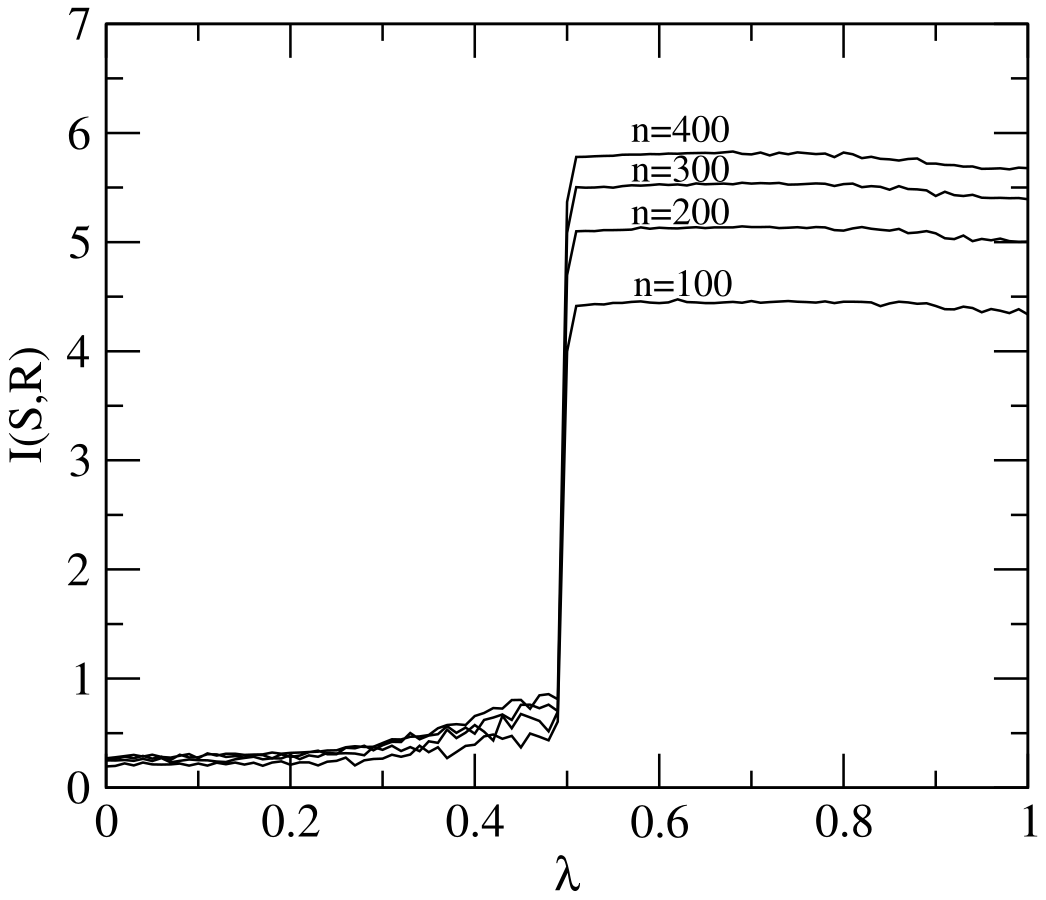
\includegraphics[width=\textwidth,height=.35\textheight,keepaspectratio]{fig2_2005_old}}
  \addjankysubfigure{b)}{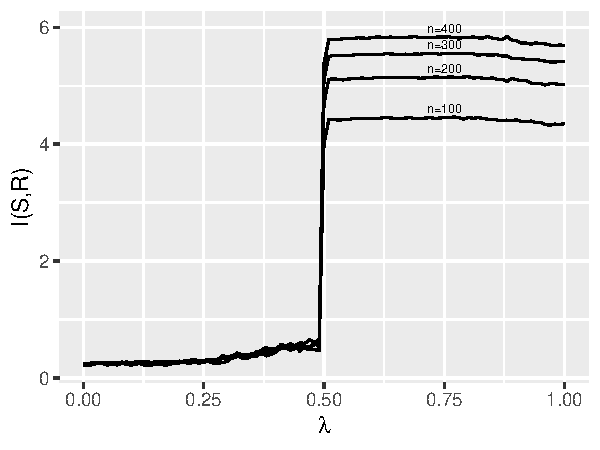
\includegraphics[width=\textwidth,height=.35\textheight,keepaspectratio]{figure2_article_EPJ_B_2005}}
  \caption{
    The mutual information $I(S,R)$ is in the $y$ axis and the $\lambda$ parameter on the $x$ axis.
    Graphs of different sizes are shown, $n=m=100$, $n=m=200$, $n=m=300$, $n=m=400$.
    Averages over 30 realizations.
    $\phi=0$, the initial graph is \randgraph{n}{m}{\frac{1}{n}}, each iteration of the optimization algorithm performs 2 mutations on the graph, the weak stop condition is used to stop the optimization process, unlinked objects are allowed.\\
    Subfigure a corresponds with Figure 2 from \cite{Ferrer2005a}.\\
    Subfigure b is the recreation of that same figure.
  }
  \label{fig:fig2_2005}
\end{figure}

\begin{figure}
  \addjankysubfigure{a)}{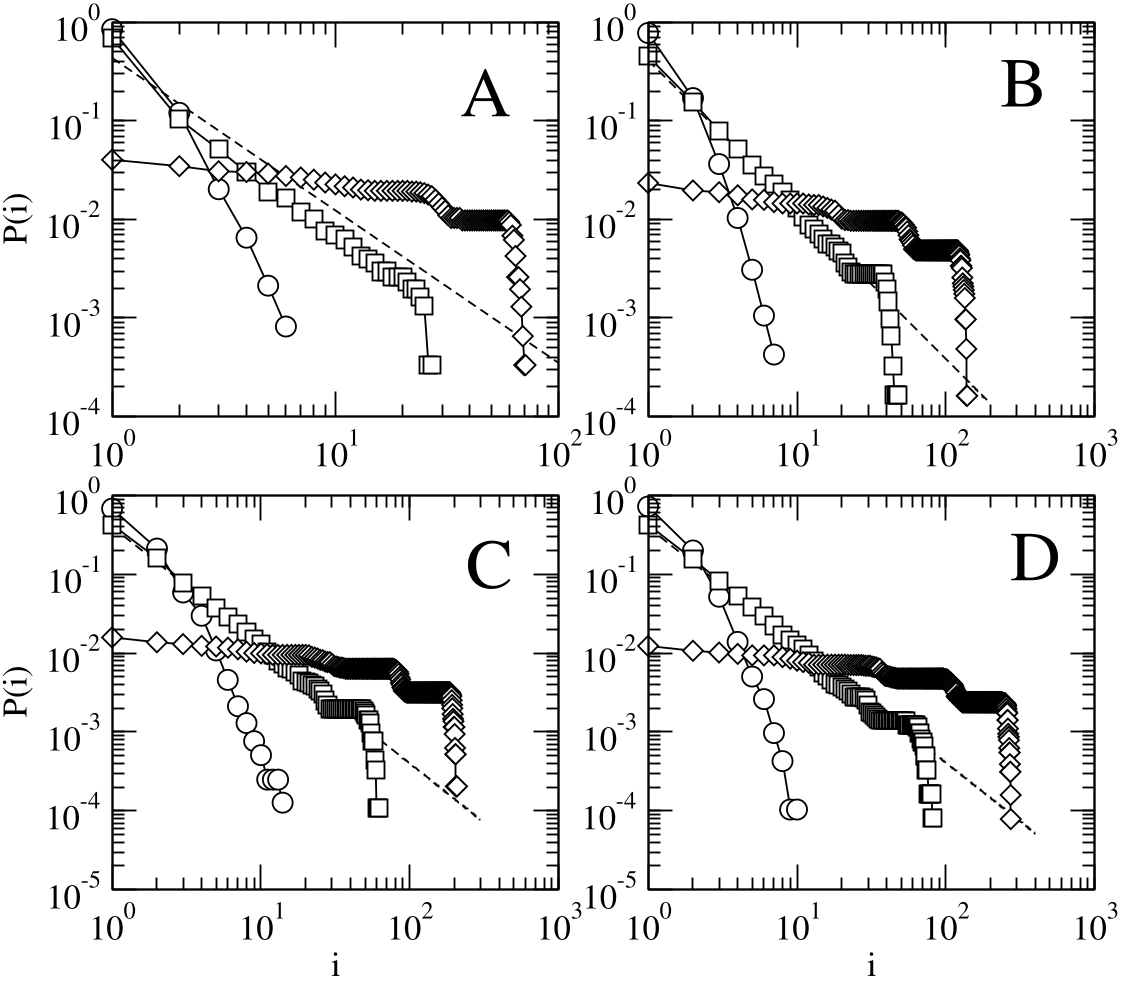
\includegraphics[width=\textwidth,height=.3\textheight,keepaspectratio]{fig3_2005_old}}
  \addjankysubfigure{b)}{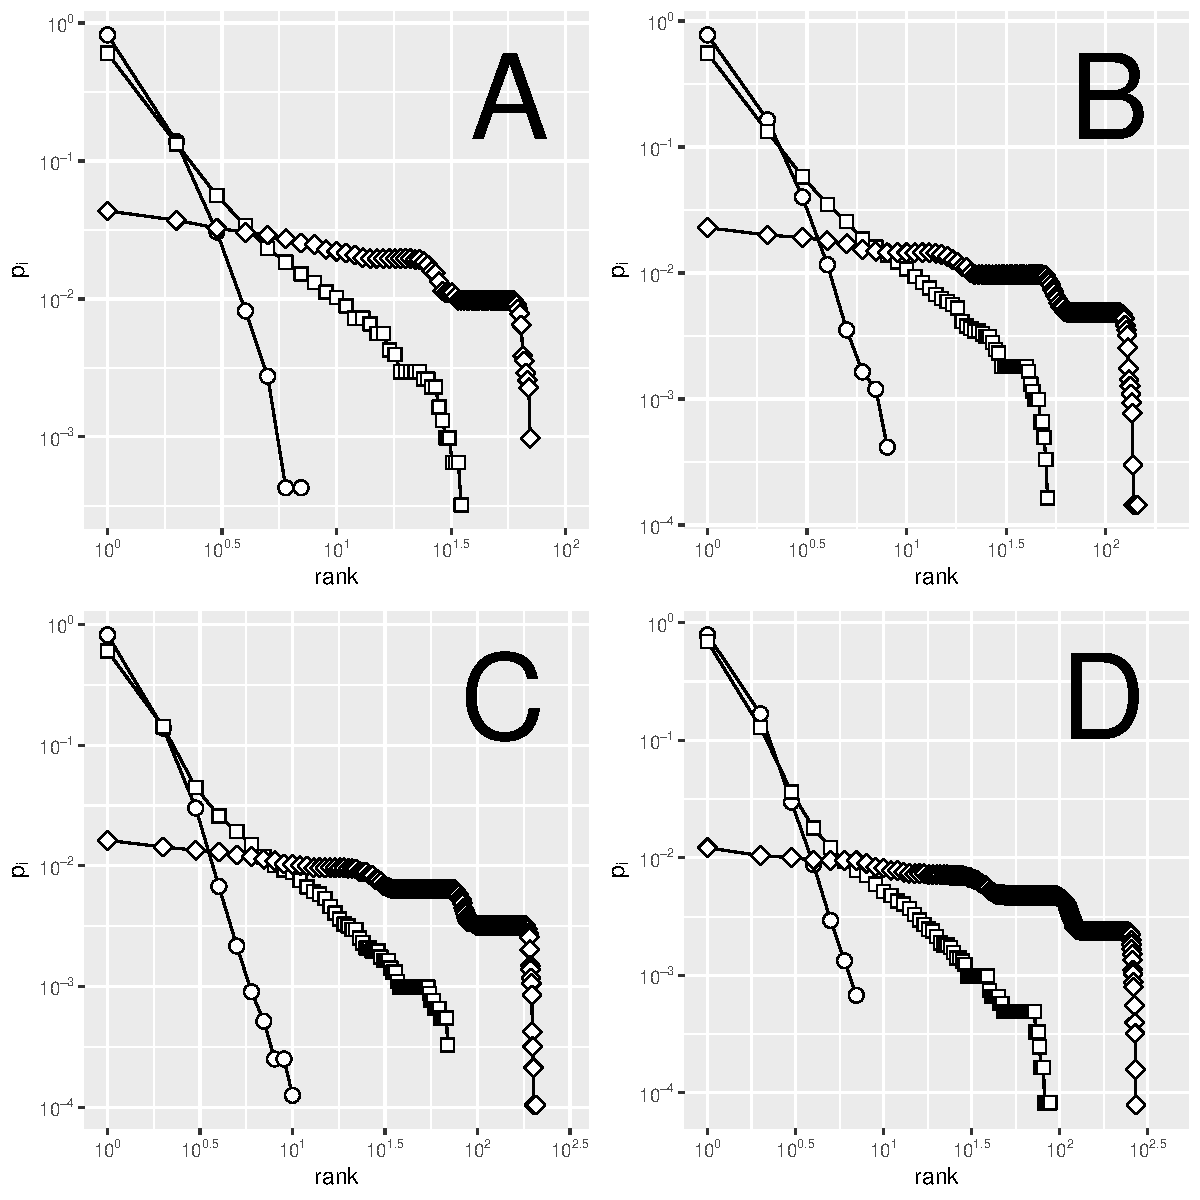
\includegraphics[width=\textwidth,height=.3\textheight,keepaspectratio]{figure3_article_EPJ_B_2005}}
  \caption{
    $P(i)$, the probability of the $i$th most frequent signal, obtained from minimum energy configurations for systems of sizes $n=m=100$ (A), $n=m=200$ (B), $n=m=300$ (C), $n=m=400$ (D).
    Four series are shown in each plot, $\lambda=0.49$ (circles), $\lambda=\lambda^*$ (squares) and $\lambda=0.5$ (diamonds) and the ideal curve for $\alpha^*$.
    Averages over 30 realizations.
    When $\lambda=\lambda^*$, $\alpha^* = 1.54$ for $n=m=100$, $\alpha^* = 1.51$ for $n=m=200$, $\alpha^* = 1.5$ for $n=m=300$ and $\alpha^* = 1.49$ for $n=m=400$.
    It was chosen that $\lambda^* = 0.4986$ for $n=m=100$, $\lambda^* = 0.4987$ for $n=m=200$, $\lambda^* = 0.4987$ for $n=m=300$, and $\lambda^* = 0.4986$ for $n=m=400$.
    Averages over 30 realizations.
    $\phi=0$, the initial graph is \randgraph{n}{m}{\frac{1}{n}}, each iteration of the optimization algorithm performs 2 mutations on the graph, the weak stop condition is used to stop the optimization process, unlinked objects are allowed.\\
    Subfigure a corresponds with Figure 3 from \cite{Ferrer2005a}.\\
    Subfigure b is the recreation of that same figure.
  }
  \label{fig:fig3_2005}
\end{figure}

Figure \ref{fig:fig2_2005} shows both the original Figure 2 from \cite{Ferrer2005a} and a recreation of this figure using the new tool.
Figure \ref{fig:fig3_2005} shows both the original Figure 3 from \cite{Ferrer2005a} and a recreation of this figure, also generated using the new tool.

The initial graph was not specified in \cite{Ferrer2005a} and a \randgraph{n}{m}{\frac{1}{n}} ($n=m$) graph is used in the replication.
The paper also does not specify how to stop the optimization process and so the weak stop condition (Section \ref{sec:methods_optimization}) is used.

Subfigures a and b from Figure \ref{fig:fig2_2005} are nearly identical.
In Figure \ref{fig:fig3_2005}, subfigures a and b are also qualitatively very similar.
Although some of the points can be seen to be not quite in the same place.

\subsection{Results from the \secondmodel{} (2003)}
\label{sec:results_verification_second}

\begin{figure}
  \addjankysubfigure{a)}{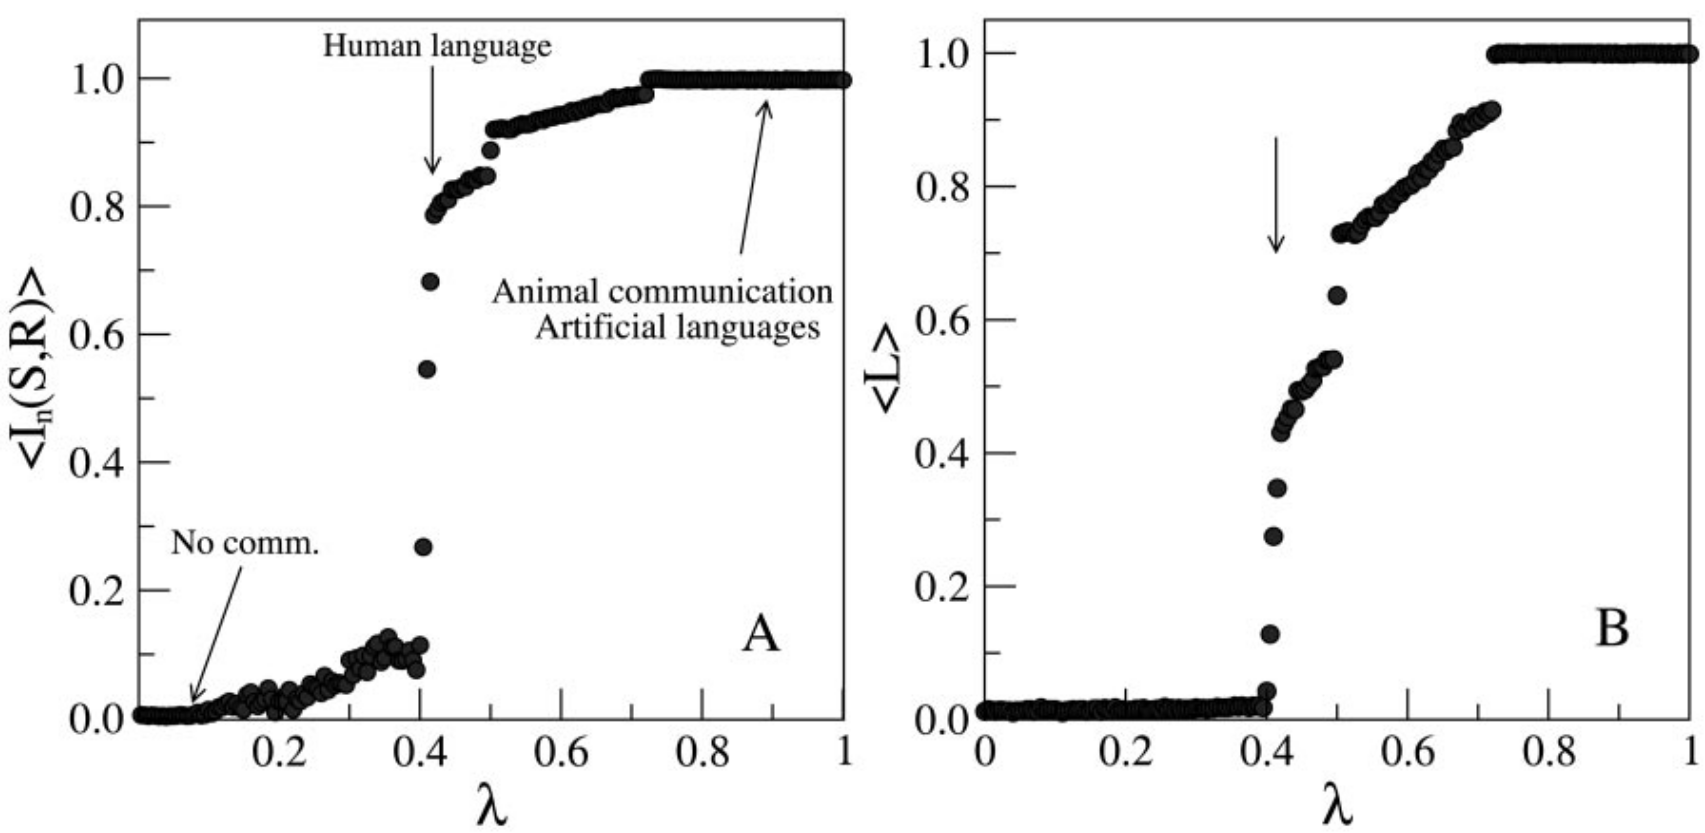
\includegraphics[width=\textwidth]{fig2_2003_old}}
  \addjankysubfigure{b)}{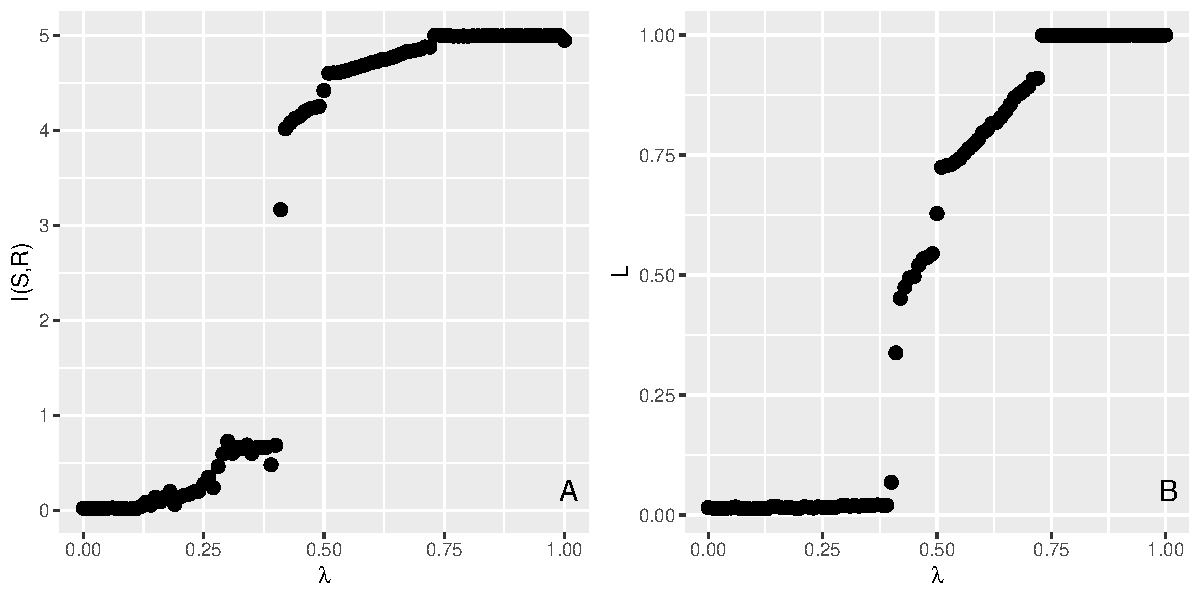
\includegraphics[width=\textwidth]{figure2_article_PNAS_2003_binom1.75}}
  \caption{
    In A, $I(S,R)$ is the mutual information obtained for values of $\lambda$ between 0 and 1.
    In B, $L$ is the lexicon size obtained for values of $\lambda$ between 0 and 1.
    An abrupt change is seen for $\lambda \approx 0.41$ in both A and B.
    Averages over 30 replicas.
    $n=m=150$, $\phi=0$, unlinked objects are not allowed, $\pi$ follows a uniform distribution.\\
    Subfigure a corresponds with Figure 2 from \cite{Ferrer2003a}\\
    Subfigure b is the recreation of that same figure using the open source tool created for this thesis.
  }
  \label{fig:fig2_2003}
\end{figure}

\begin{figure}
  \addjankysubfigure{a)}{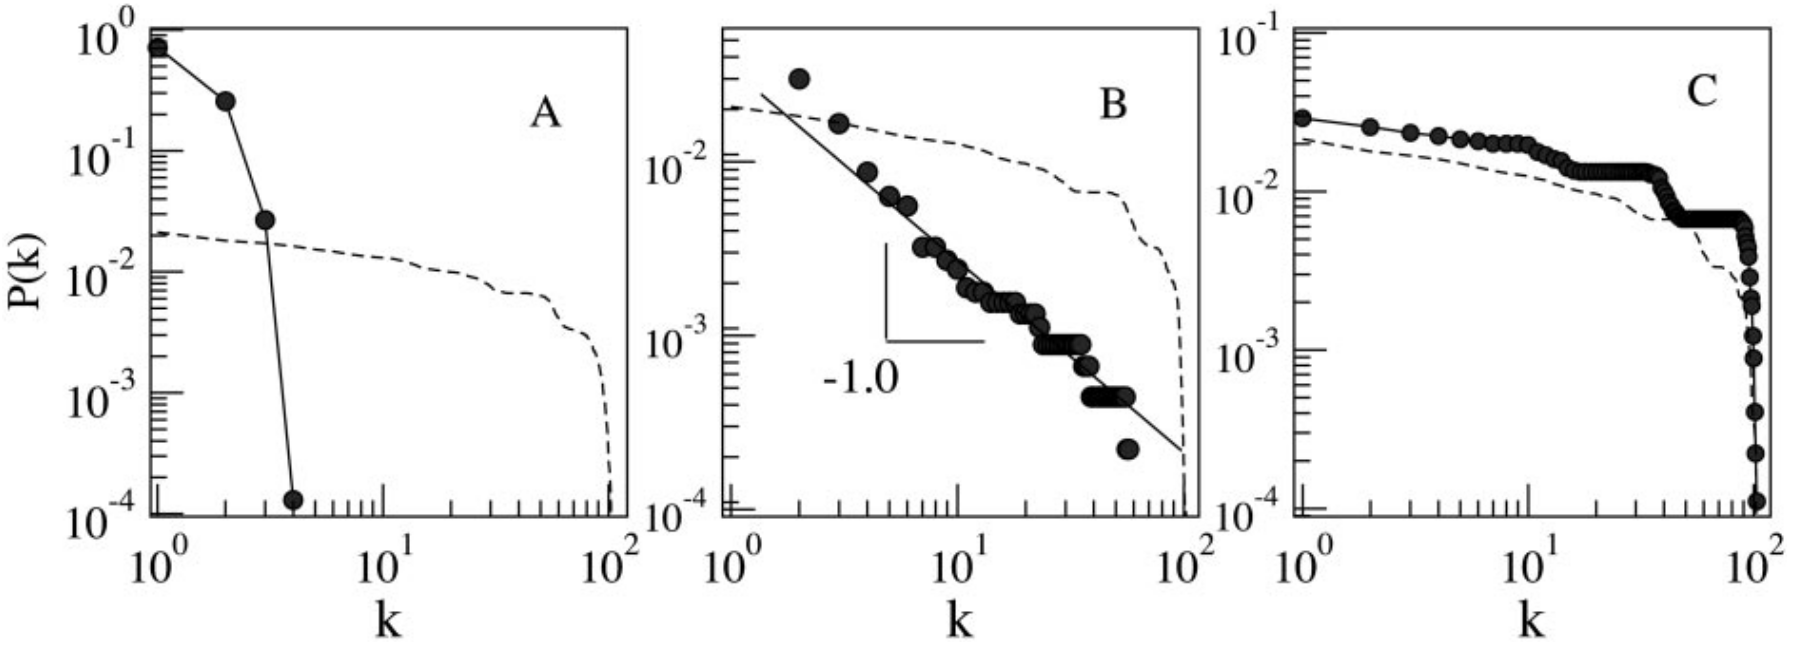
\includegraphics[width=\textwidth]{fig3_2003_old}}
  \addjankysubfigure{b)}{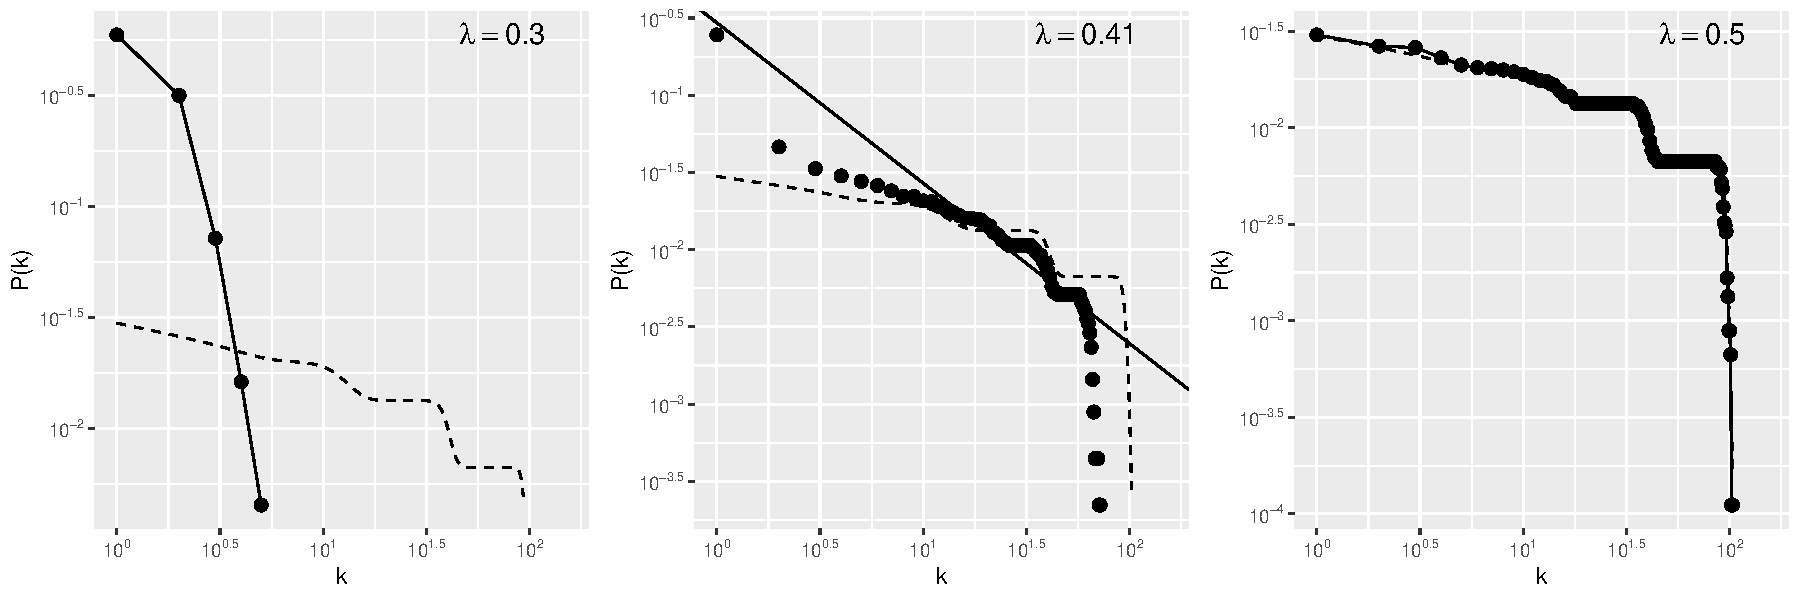
\includegraphics[width=\textwidth]{figure3_article_PNAS_2003_binom1.75}}
  \caption{
    Normalized signal frequency $P(k)$ versus rank $k$.
    The dashed lines show the distribution obtained when from a \randgraph{n}{m}{e^*} graph where $e^*$ is the number of connections in these optimal configurations.
    In both cases the distribution of B is still consistent with human language, $\alpha=1$.
    Averages over 30 replicas, $n=m=150$, the initial graph is \randgraph{n}{m}{\frac{10}{n}}, the number of mutations on each iteration follows a binomial distribution with average 1.75, the optimization stops after $2nm$ mutations that do not improve the cost function.\\
    Above: Figure 3 from \cite{Ferrer2003a}\\
    Below: Recreation of that same figure using the open source tool created for this thesis.
  }
  \label{fig:fig3_2003}
\end{figure}

Figure \ref{fig:fig2_2003} shows both the original Figure 2 from \cite{Ferrer2003a} and the recreation of this figure using the new tool.
Figure \ref{fig:fig3_2003} shows the original Figure 3 from \cite{Ferrer2003a} and a recreation using the new tool.

The initial graph was specified as a \randgraph{n}{m}{\rho} but the value of $\rho$ was not given in the paper, a \randgraph{n}{m}{\frac{10}{n}} graph was used (that is, a value of $\rho=\frac{10}{n}$).
It is specified that the number of mutations done on each iteration of the optimization algorithm follows a binomial distribution.
However it was later found that, due to a bug in the generator of binomial numbers, the number of mutations must have been lower.
Several values were tried for the average number of binomial mutations, with 1.75 giving the results most similar to the previous model's.

Qualitatively, it seems that the two subfigures in Figure \ref{fig:fig2_2003} are very similar.
Some of the points in A do not form exactly the same shape, however, and it seems that not as many points appear inside the phase transition.
As for Figure \ref{fig:fig3_2003}, subfigures A and C are quite similar (although the dashed line appears to overlap the data in subfigure b more than it did in a).
Subfigure B is not as similar.
However, the slope of the curve is also 1.0 as indicated by the solid line.

\section{Results for current models}
\label{sec:results_new}

Here aspects of these models that had not been considered before are investigated, such as untested linguistic laws or regions of their parameter space.
All results presented here come from the minimization of the cost function (Equation \eqref{eq:definition-Omega}).
Firstly, and as a way to for an intuition of the kinds of graphs that these models generate, Section \ref{sec:results_new_graph} presents the optimal graphs for different initial conditions for both models.
Section \ref{sec:results_new_other} shows the rest of the obtained results.
This section focuses first on plots of the values obtained for the information theoretical measures of the optimal graphs for various value of $\lambda$ in the cost function.
As a reminder, $\lambda$ controls the weight of either the entropy or the mutual information in the cost function.
Statistical measures for select values of $\lambda$ are then shown.
These measures show how various linguistic laws are recovered in the results.
Several kinds of initial graphs are shown throughout this section.
\begin{redenv}
  For each of the four models (\firstmodel{} with $\phi=0$ and $\phi\neq 0$, \secondmodel with $\phi=0$ and $\phi\neq 0$) studied, several initial conditions are shown.
  The aim is to investigate how these particular initial conditions can influence the development of the model.
\end{redenv}

\begin{redenv}
  \begin{itemize}
  \item Random: The initial graph is a \randgraph{n}{m}{\frac{3}{nm}} random graph.
  \item Single link: The initial graph contains a single link between a word and a meaning. \redtxt{This initial condition is also a global minimum of the cost function for $\lambda \leq \frac{1}{2}$ (See Section \ref{TODO})}
  \item One-to-one: The initial graph is a bijection connecting words and meanings one to one,
    \redtxt{which is a minimum of the cost function when $\lambda \geq \frac{1}{2}$ (Section \ref{TODO})}
  \item Complete: The initial graph is a complete bipartite graph where every word connects to every meaning and every meaning to every word. \redtxt{This is a maximum of the cost function.}
  \end{itemize}
\end{redenv}

All results in this section perform two mutations on each iteration of the optimization algorithm, which stops with the \emph{weak} stop condition.
See Section \ref{sec:methods_optimization} for more information on the optimization process.

\subsection{Graph visualization}
\label{sec:results_new_graph}

Here various graphs are plotted.
They correspond to graphs of size $n=m=60$ and $\phi=1$.
\begin{redenv}
  The graph is initialized with some initial condition and then the optimization process is executed.
  The presented graph is the result of this optimization process.
\end{redenv}
Unlinked meanings are also allowed in all graphs.
It is interesting to see the different shapes the graph takes for different values of $\lambda$.

For the first model, four graphs are shown.

\begin{redenv}
  \begin{itemize}
  \item Random initial graph, Figure \ref{fig:graphVisualization_firstModel_phi1_nm60_static_randomBipartite_allowUnlinked}.
    For lower values of $\lambda$ a single word dominates, becoming linked to almost every meaning.
    For greater values of $\lambda$ more words appear linked to other meanings.
    This persists for $\lambda \leq 0.5$ is reached.
    For $\lambda=1$ the graphs are composed of long chains of connected words and meanings.
  \item Single link initial graph, Figure \ref{fig:graphVisualization_firstModel_phi1_nm60_static_singleLink_allowUnlinked}.
    A single link is maintained for $\lambda \leq 0.5$.
    After that point, the graph evolves into an almost one-to-one configuration of links between words and meanings (some words or meanings may remain unlinked).
  \item One-to-one initial graph, Figure \ref{fig:graphVisualization_firstModel_phi1_nm60_static_oneToOne_allowUnlinked}.
    The graph evolves to a configuration where a single word dominates for $\lambda < 0.5$.
    However, after $\lambda=0.5$ is reached, the graphs remain in a one-to-one configuration of links between words and meanings, which in this case becomes difficult to see as every word and every meaning are linked.
  \item Complete initial graph, Figure \ref{fig:graphVisualization_firstModel_phi1_nm60_static_complete_allowUnlinked}.
    Behaves similarly to the random initial graph, with most meanings converging on one word while all other words and meanings remain unconnected for $\lambda \leq 0.5$.
    Also for $\lambda=1$ it can be seen that the graphs are composed of long chains of connected words and meanings.
  \end{itemize}
\end{redenv}

For the second model, the \emph{a priori} probability $\pi$ follows a uniform distribution.
Four additional graphs are shown.

\begin{redenv}
  \begin{itemize}
  \item Random initial graph, Figure \ref{fig:graphVisualization_uniform_phi1_nm60_static_randomBipartite_allowUnlinked}.
    For $\lambda < 0.5$, a single word dominates and becomes connected to most meanings.
    For $\lambda \geq 0.5$ less meanings are attached to the word.
    When $\lambda$ has reached 1, it seems that a single meaning begins to dominate words, with most other words linked in a one-to-one configuration with the rest of meanings.
  \item Single link initial graph, Figure \ref{fig:graphVisualization_uniform_phi1_nm60_static_singleLink_allowUnlinked}.
    Similarly to the \firstmodel{}, the single link does not evolve and is maintained for $\lambda \leq 1$.
    When $\lambda$ has reached 1 we see the same one-to-one configuration with one dominating meaning as in the random initial condition.
  \item One-to-one initial graph, Figure \ref{fig:graphVisualization_uniform_phi1_nm60_static_oneToOne_allowUnlinked}.
    For $\lambda < 0.5$ a single word dominates, while for $\lambda \geq 0.5$ the initial condition fails to evolve into another configuration.
  \item Complete initial graph, Figure \ref{fig:graphVisualization_uniform_phi1_nm60_static_complete_allowUnlinked}.
    Presents almost the same behavior as the random initial graph, with a single dominating word at the start which weakens and, by the time $\lambda$ has reached 1, a single meaning seems to dominate instead.
  \end{itemize}
\end{redenv}

\begin{figure}
  \centering
  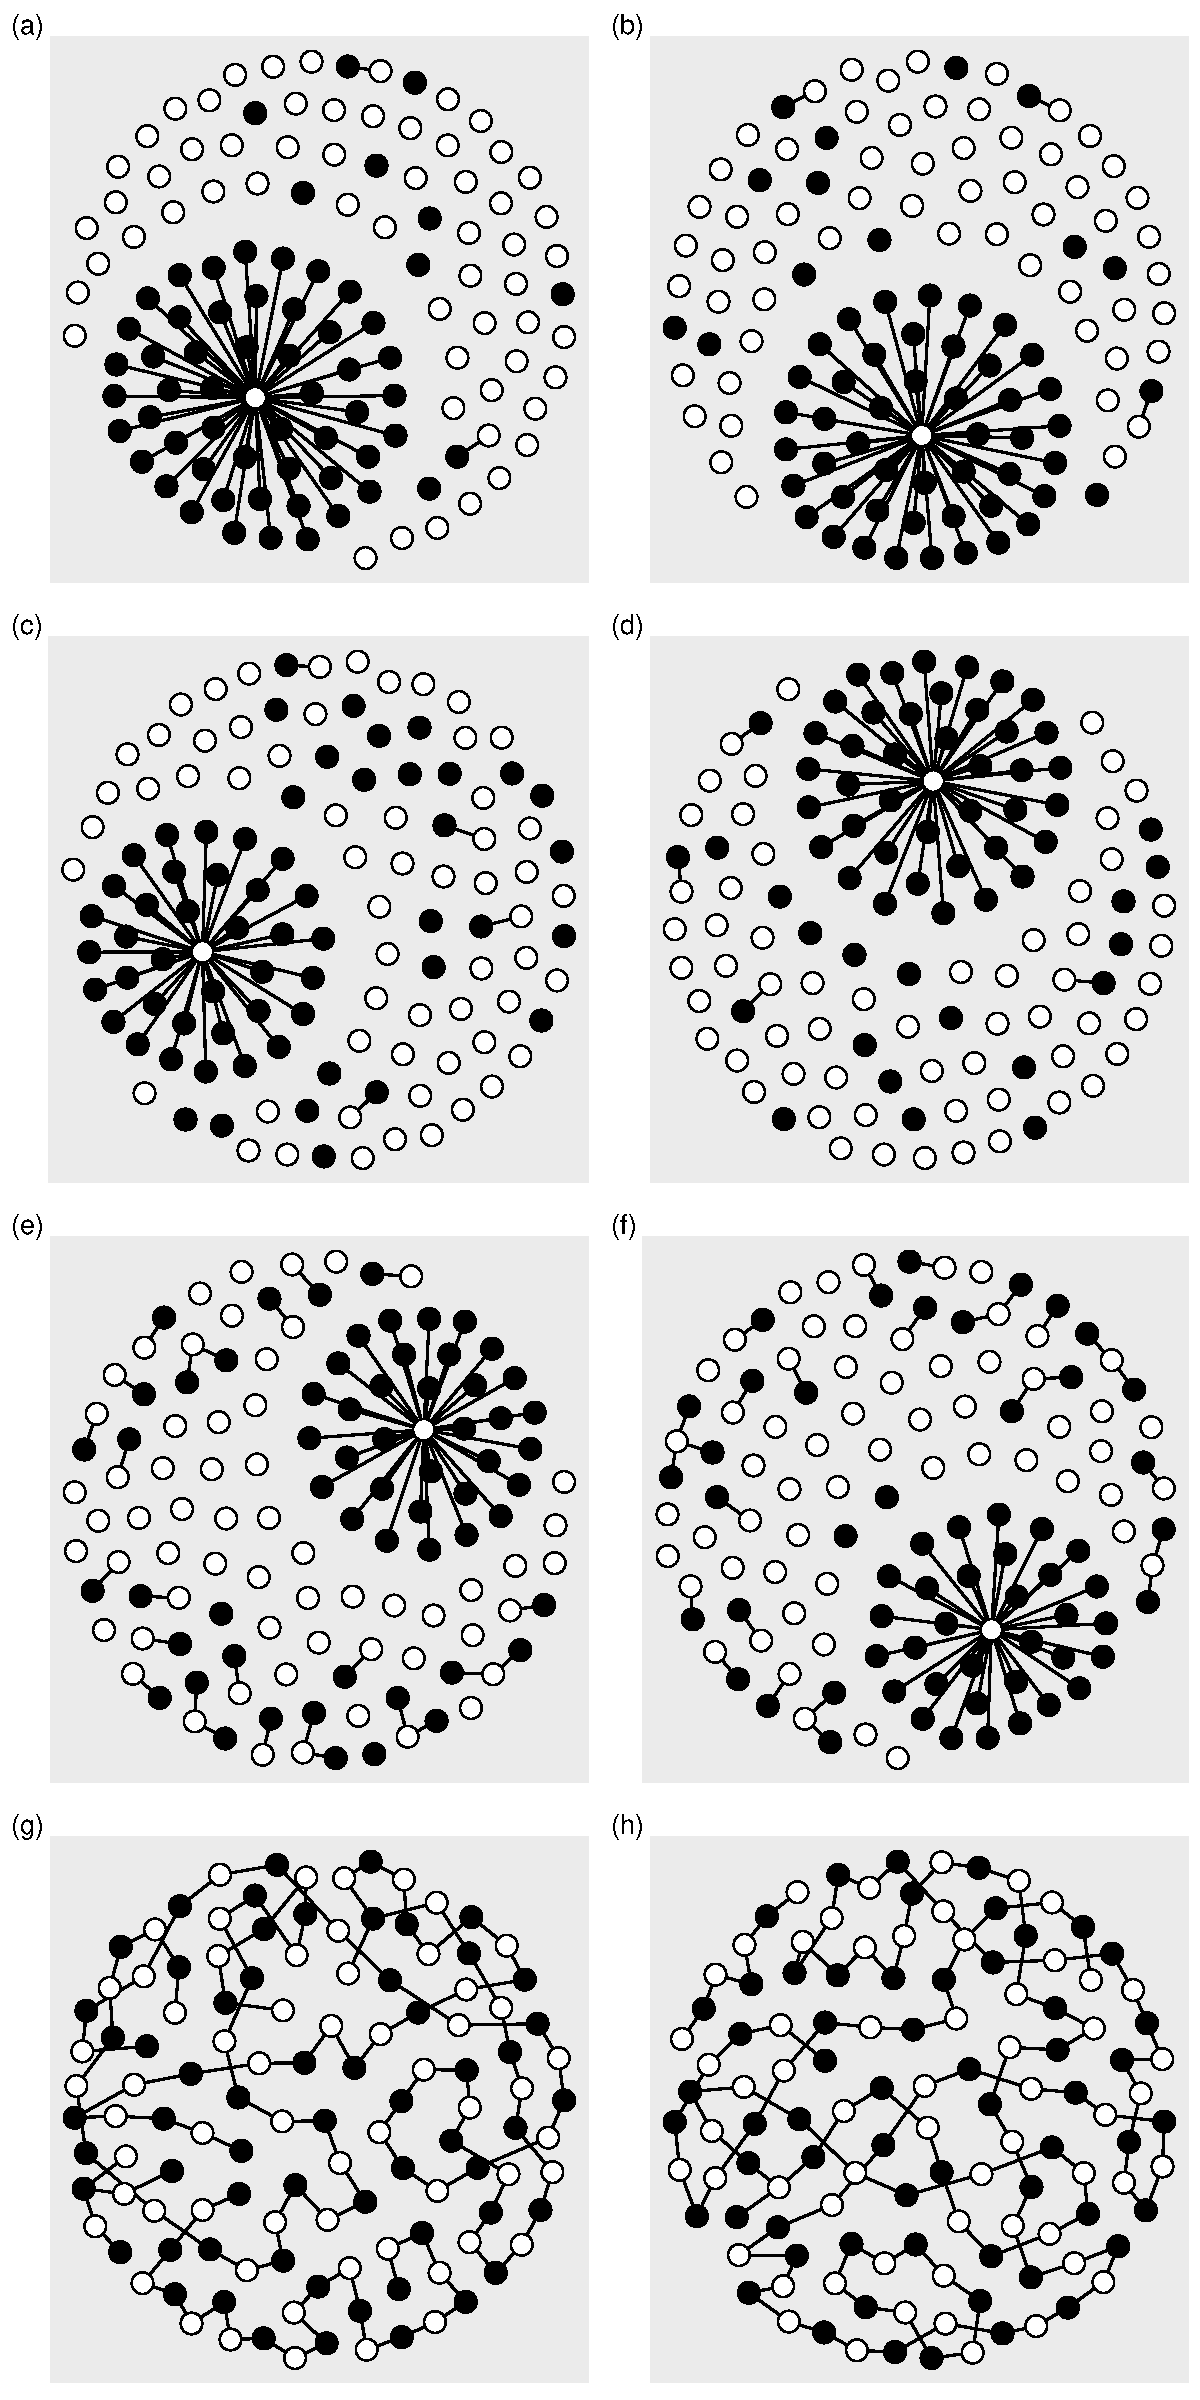
\includegraphics[height=\textheight,width=\textwidth,keepaspectratio]{graphVisualization_firstModel_phi1_nm60_static_randomBipartite_allowUnlinked}
  \caption{a}
  \label{fig:graphVisualization_firstModel_phi1_nm60_static_randomBipartite_allowUnlinked}
\end{figure}

\begin{figure}
  \centering
  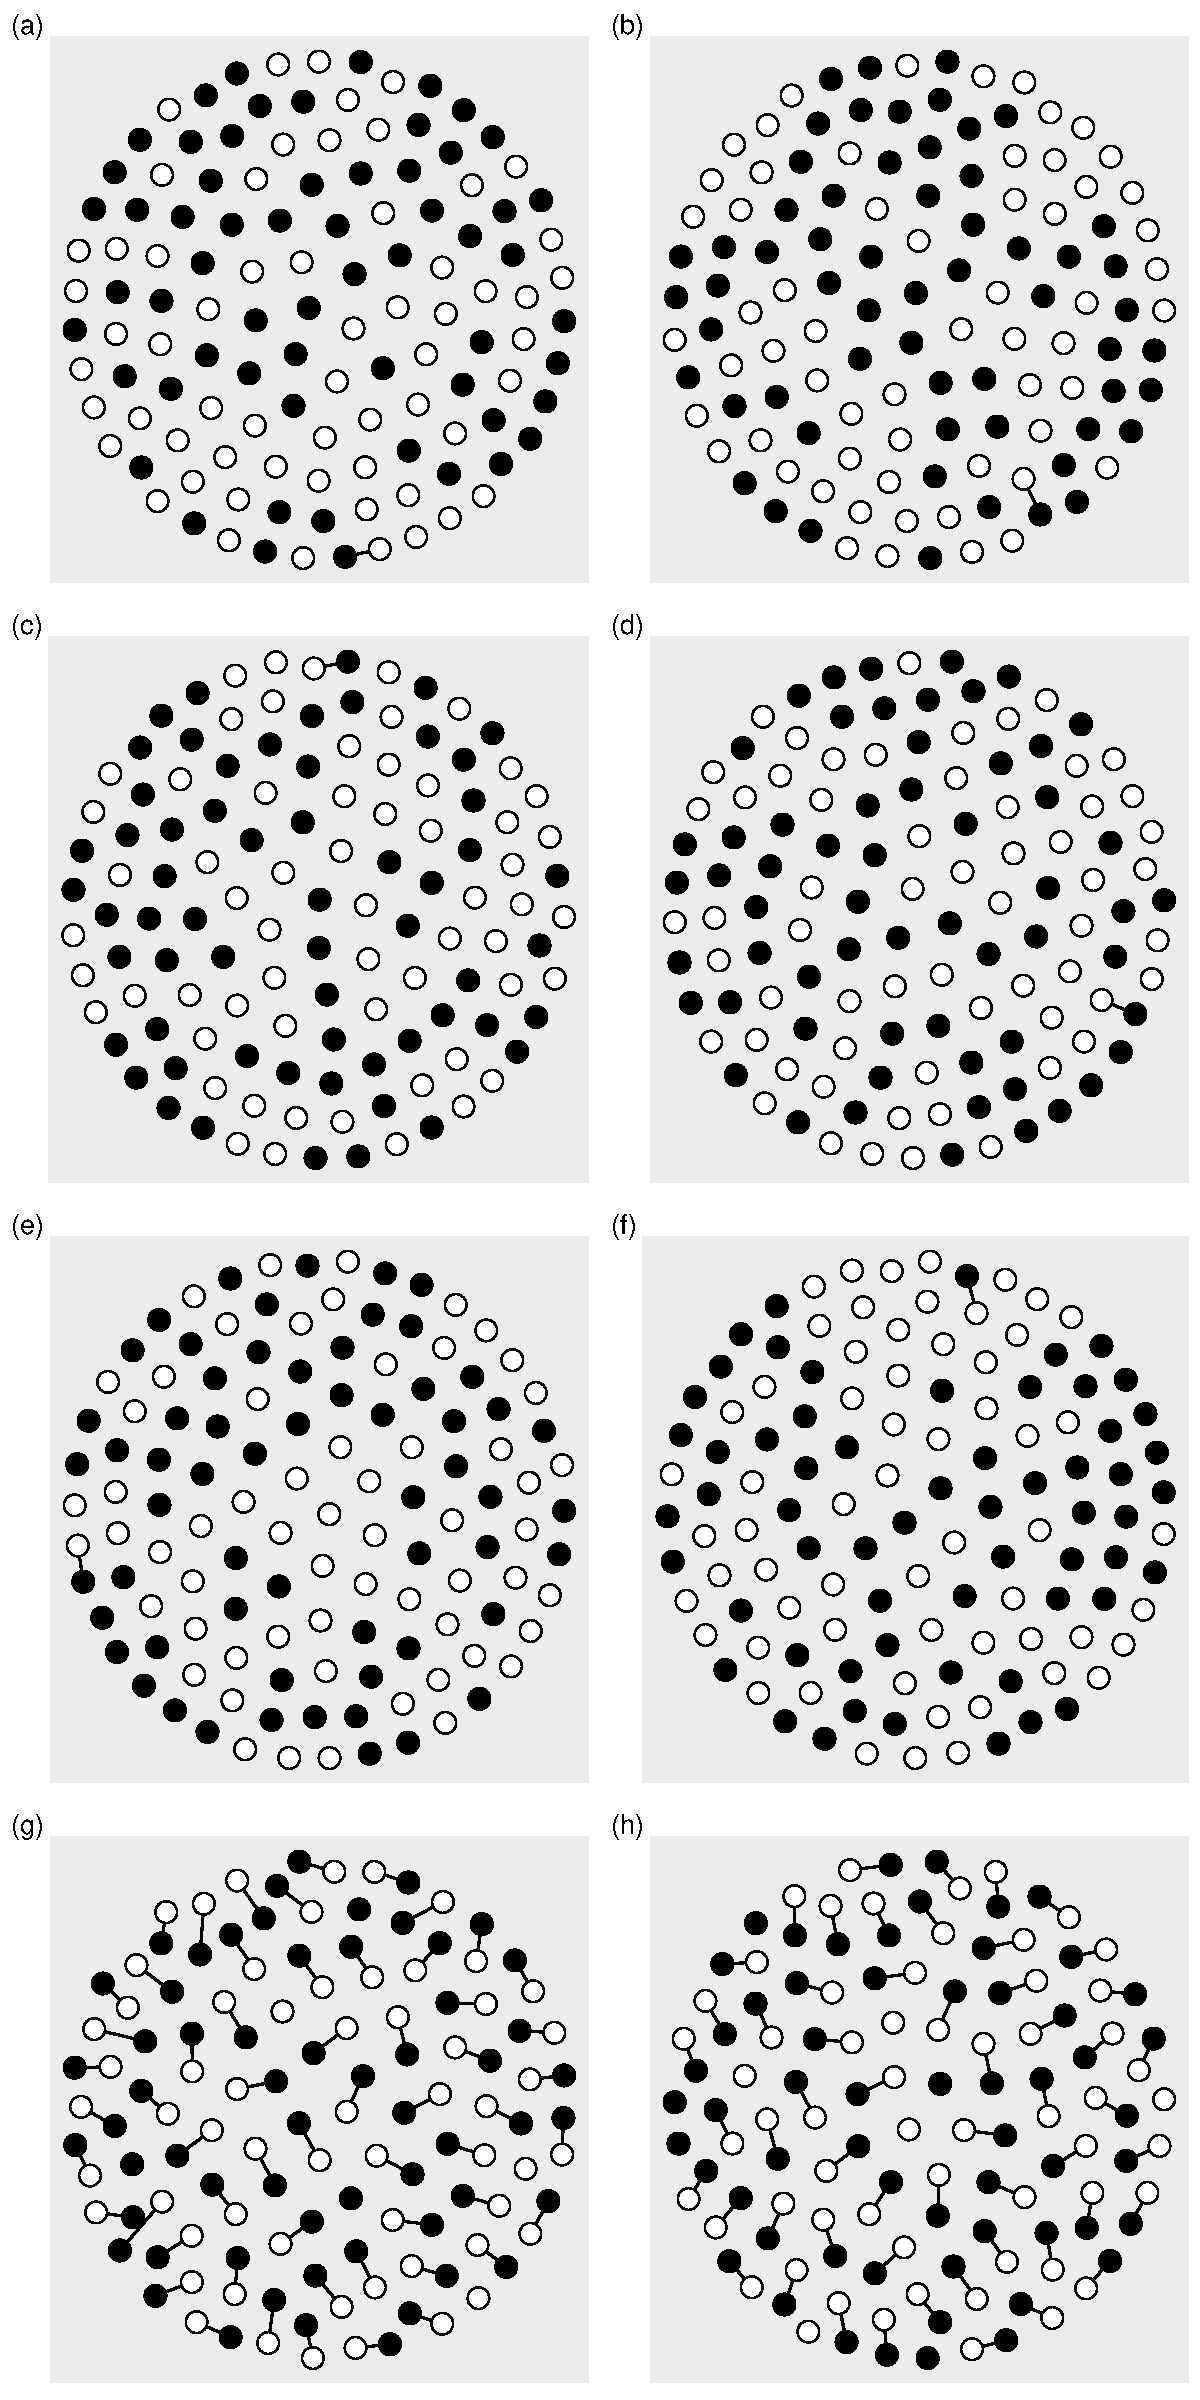
\includegraphics[height=\textheight,width=\textwidth,keepaspectratio]{graphVisualization_firstModel_phi1_nm60_static_singleLink_allowUnlinked}
  \caption{a}
  \label{fig:graphVisualization_firstModel_phi1_nm60_static_singleLink_allowUnlinked}
\end{figure}

\begin{figure}
  \centering
  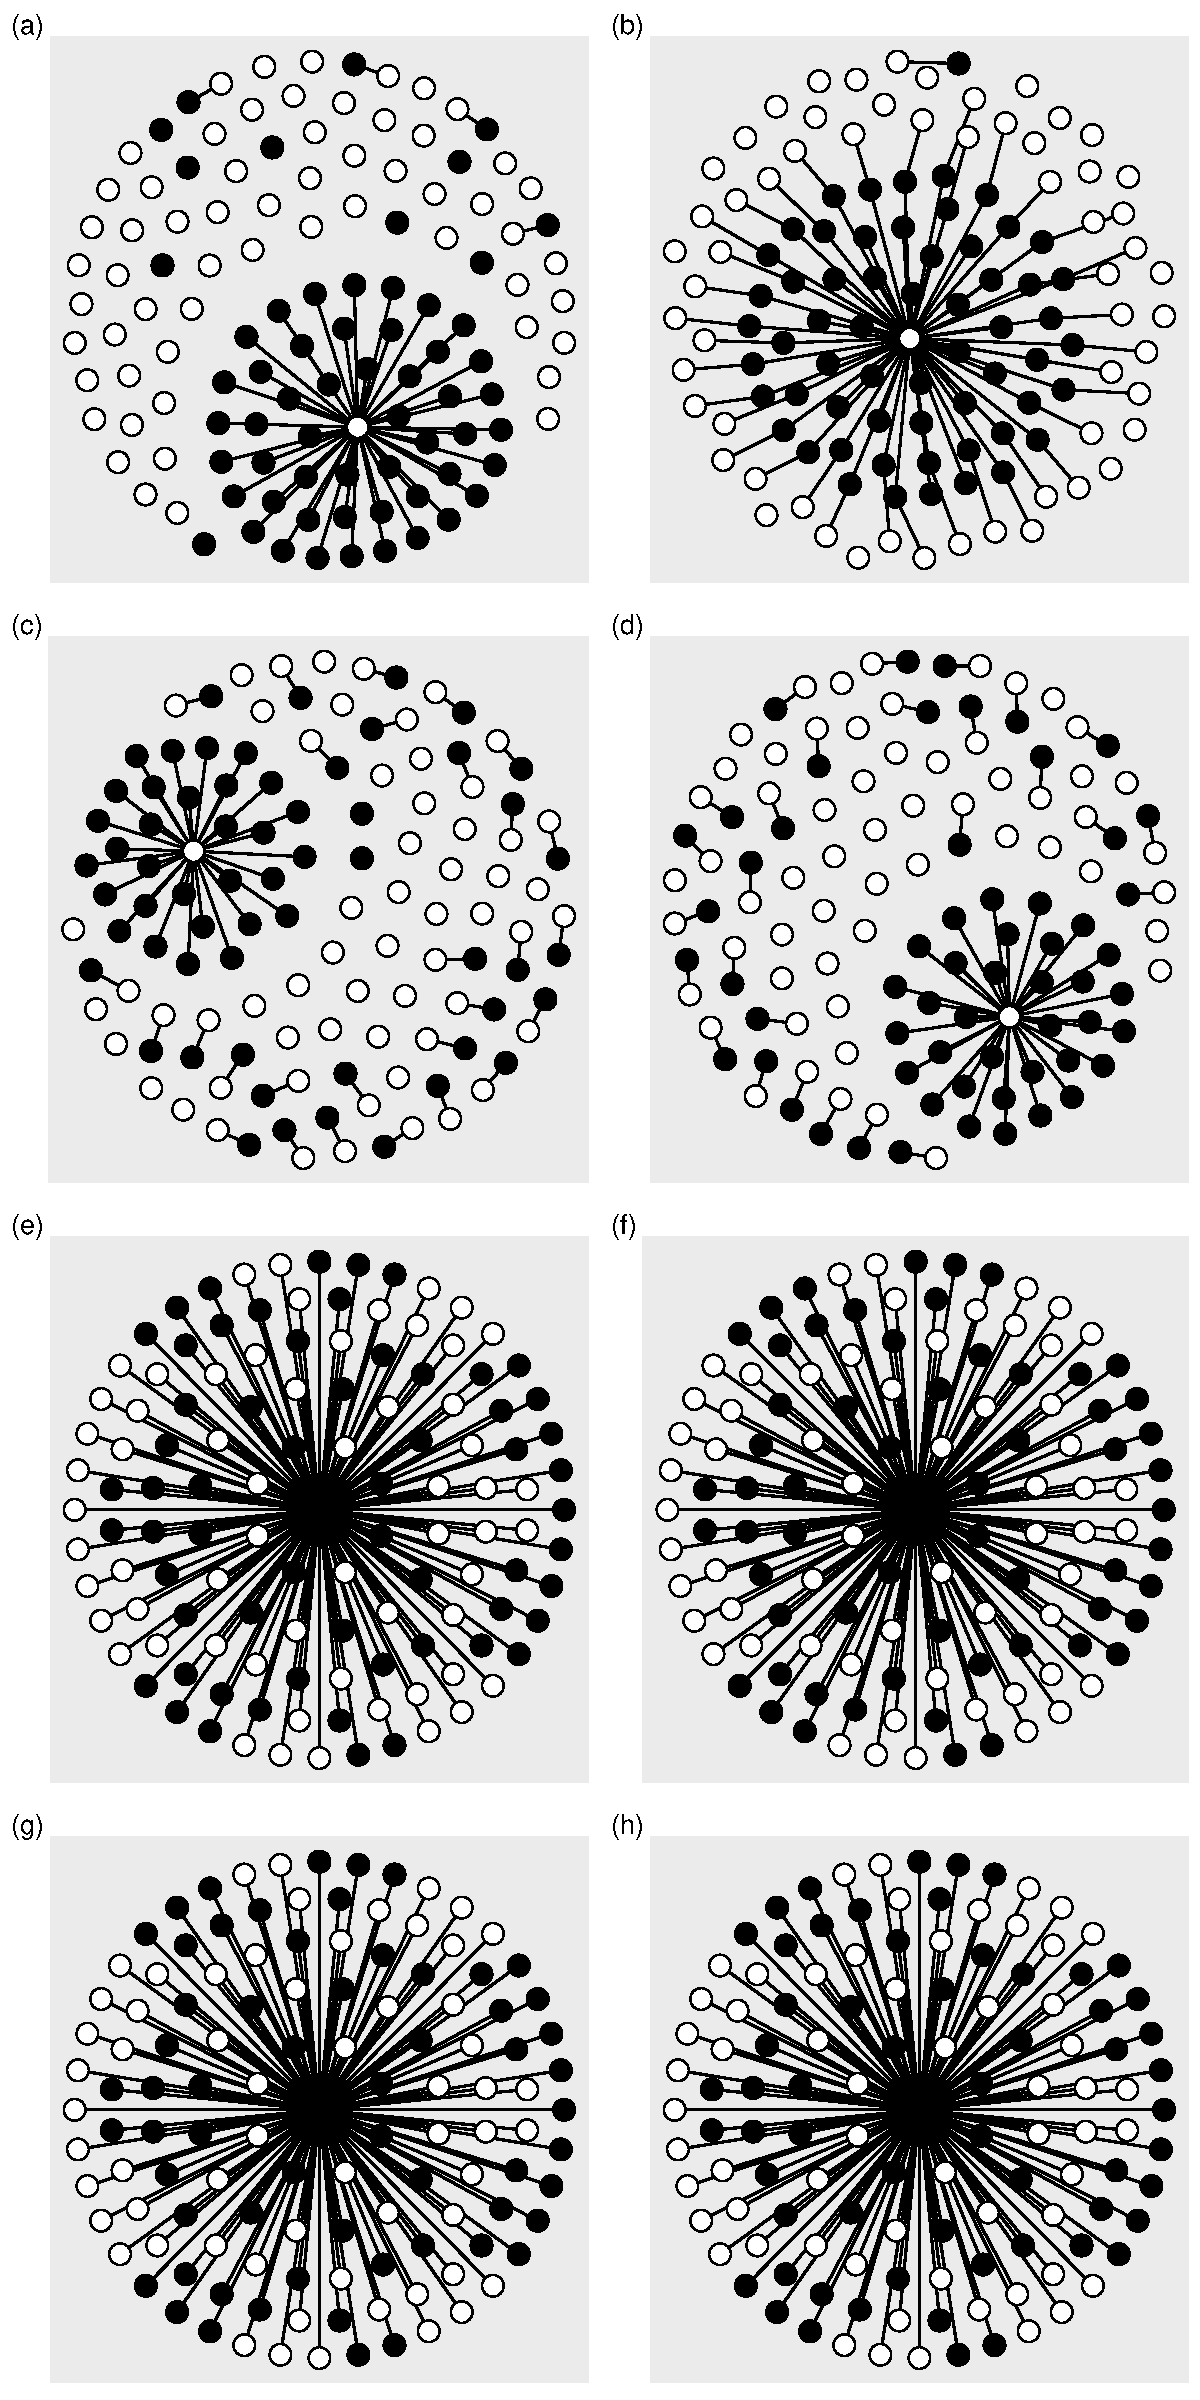
\includegraphics[height=\textheight,width=\textwidth,keepaspectratio]{graphVisualization_firstModel_phi1_nm60_static_oneToOne_allowUnlinked}
  \caption{a}
  \label{fig:graphVisualization_firstModel_phi1_nm60_static_oneToOne_allowUnlinked}
\end{figure}

\begin{figure}
  \centering
  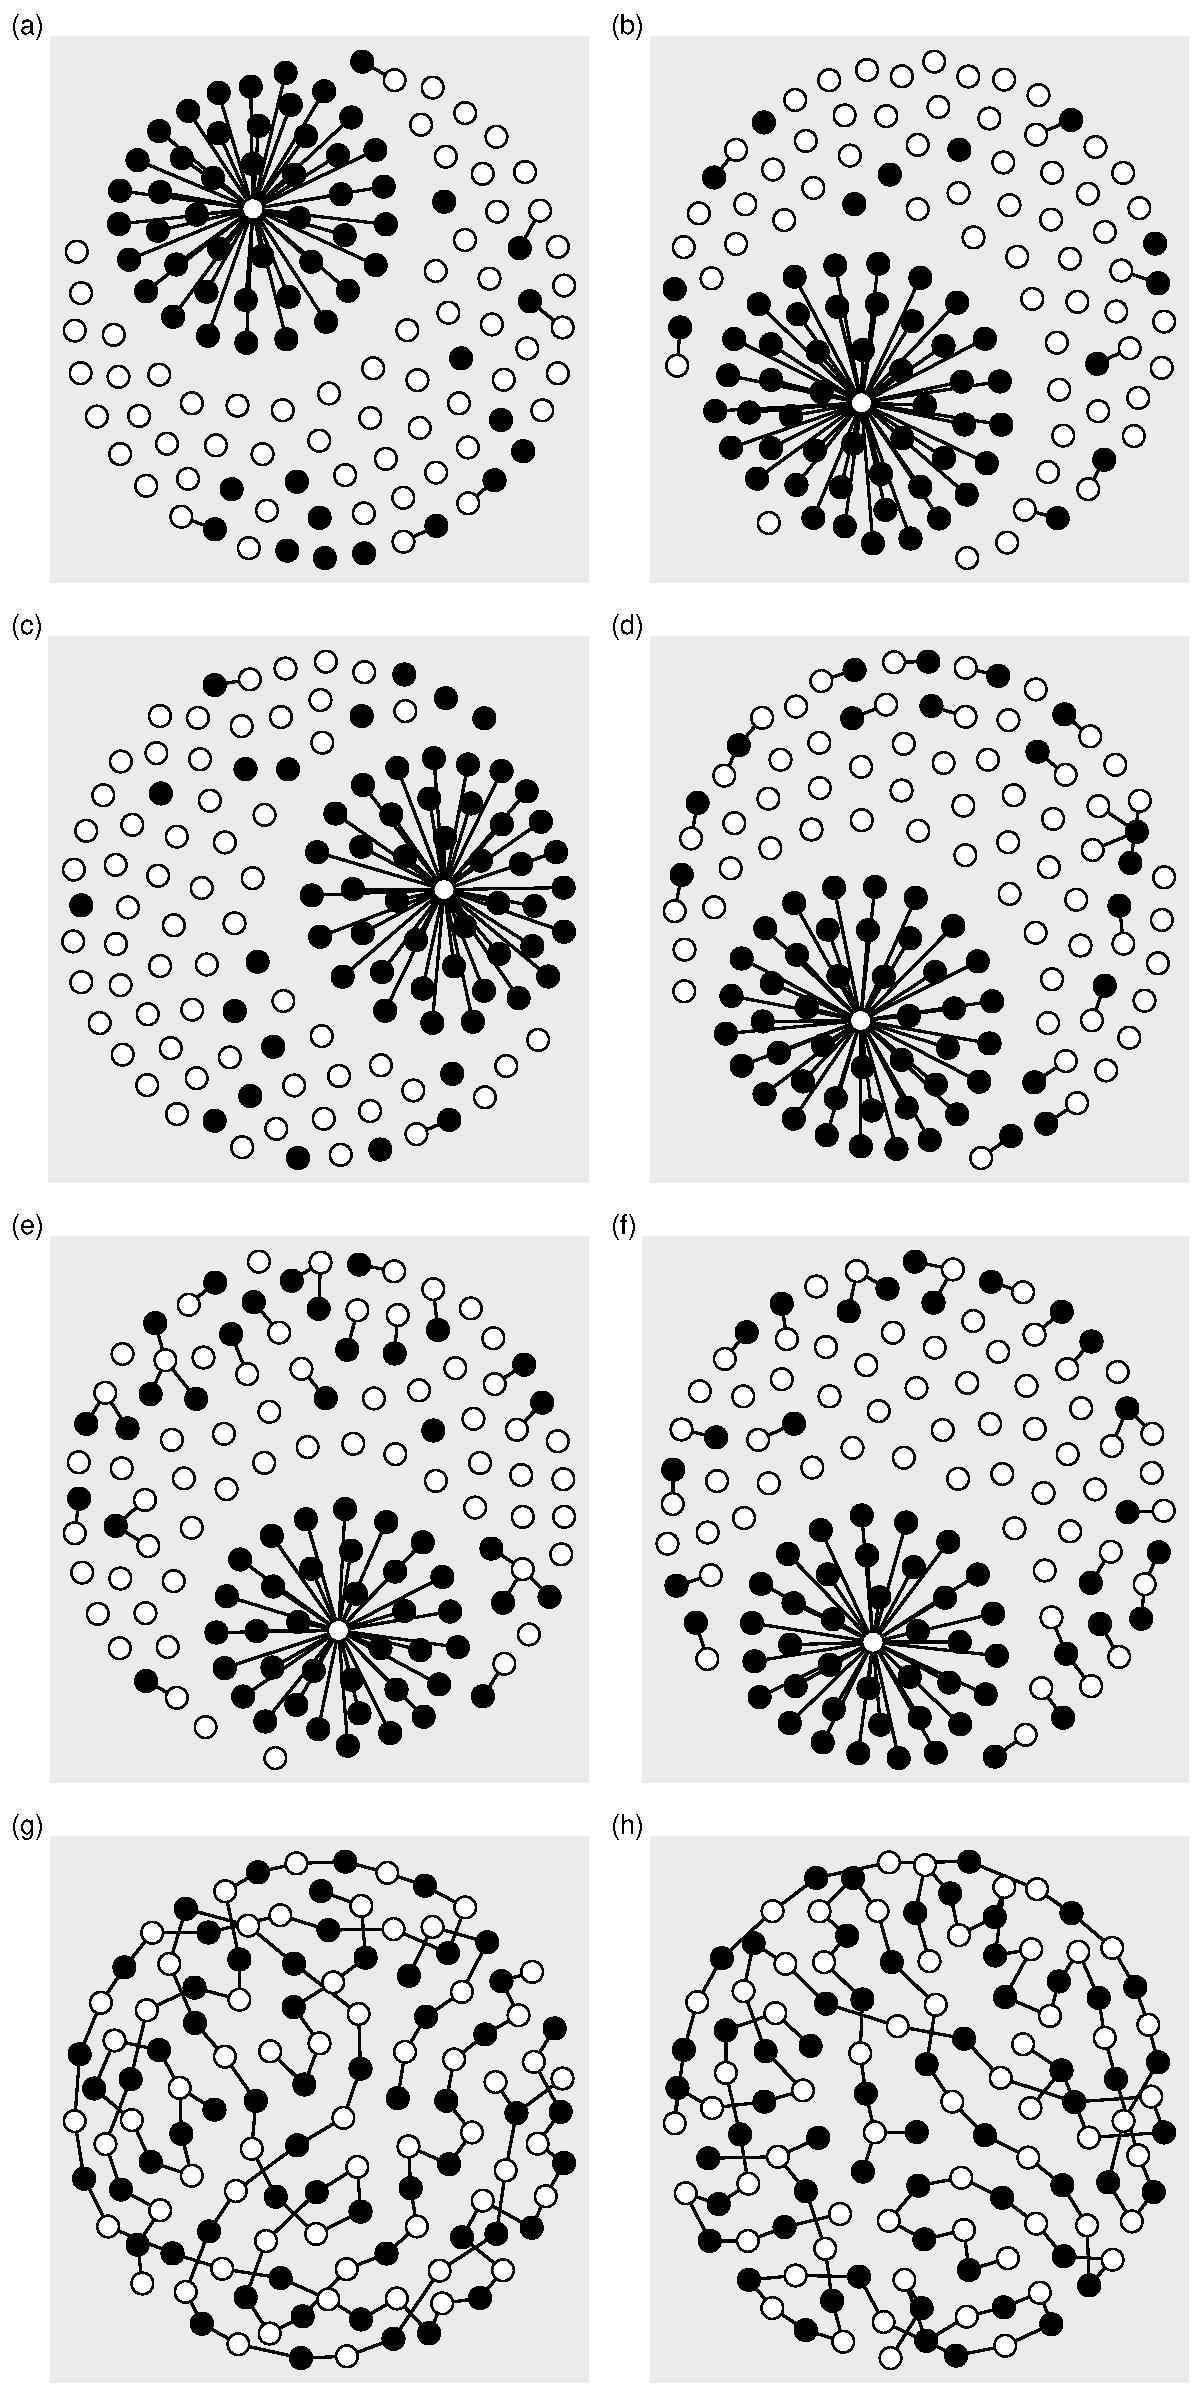
\includegraphics[height=\textheight,width=\textwidth,keepaspectratio]{graphVisualization_firstModel_phi1_nm60_static_complete_allowUnlinked}
  \caption{a}
  \label{fig:graphVisualization_firstModel_phi1_nm60_static_complete_allowUnlinked}
\end{figure}

\begin{figure}
  \centering
  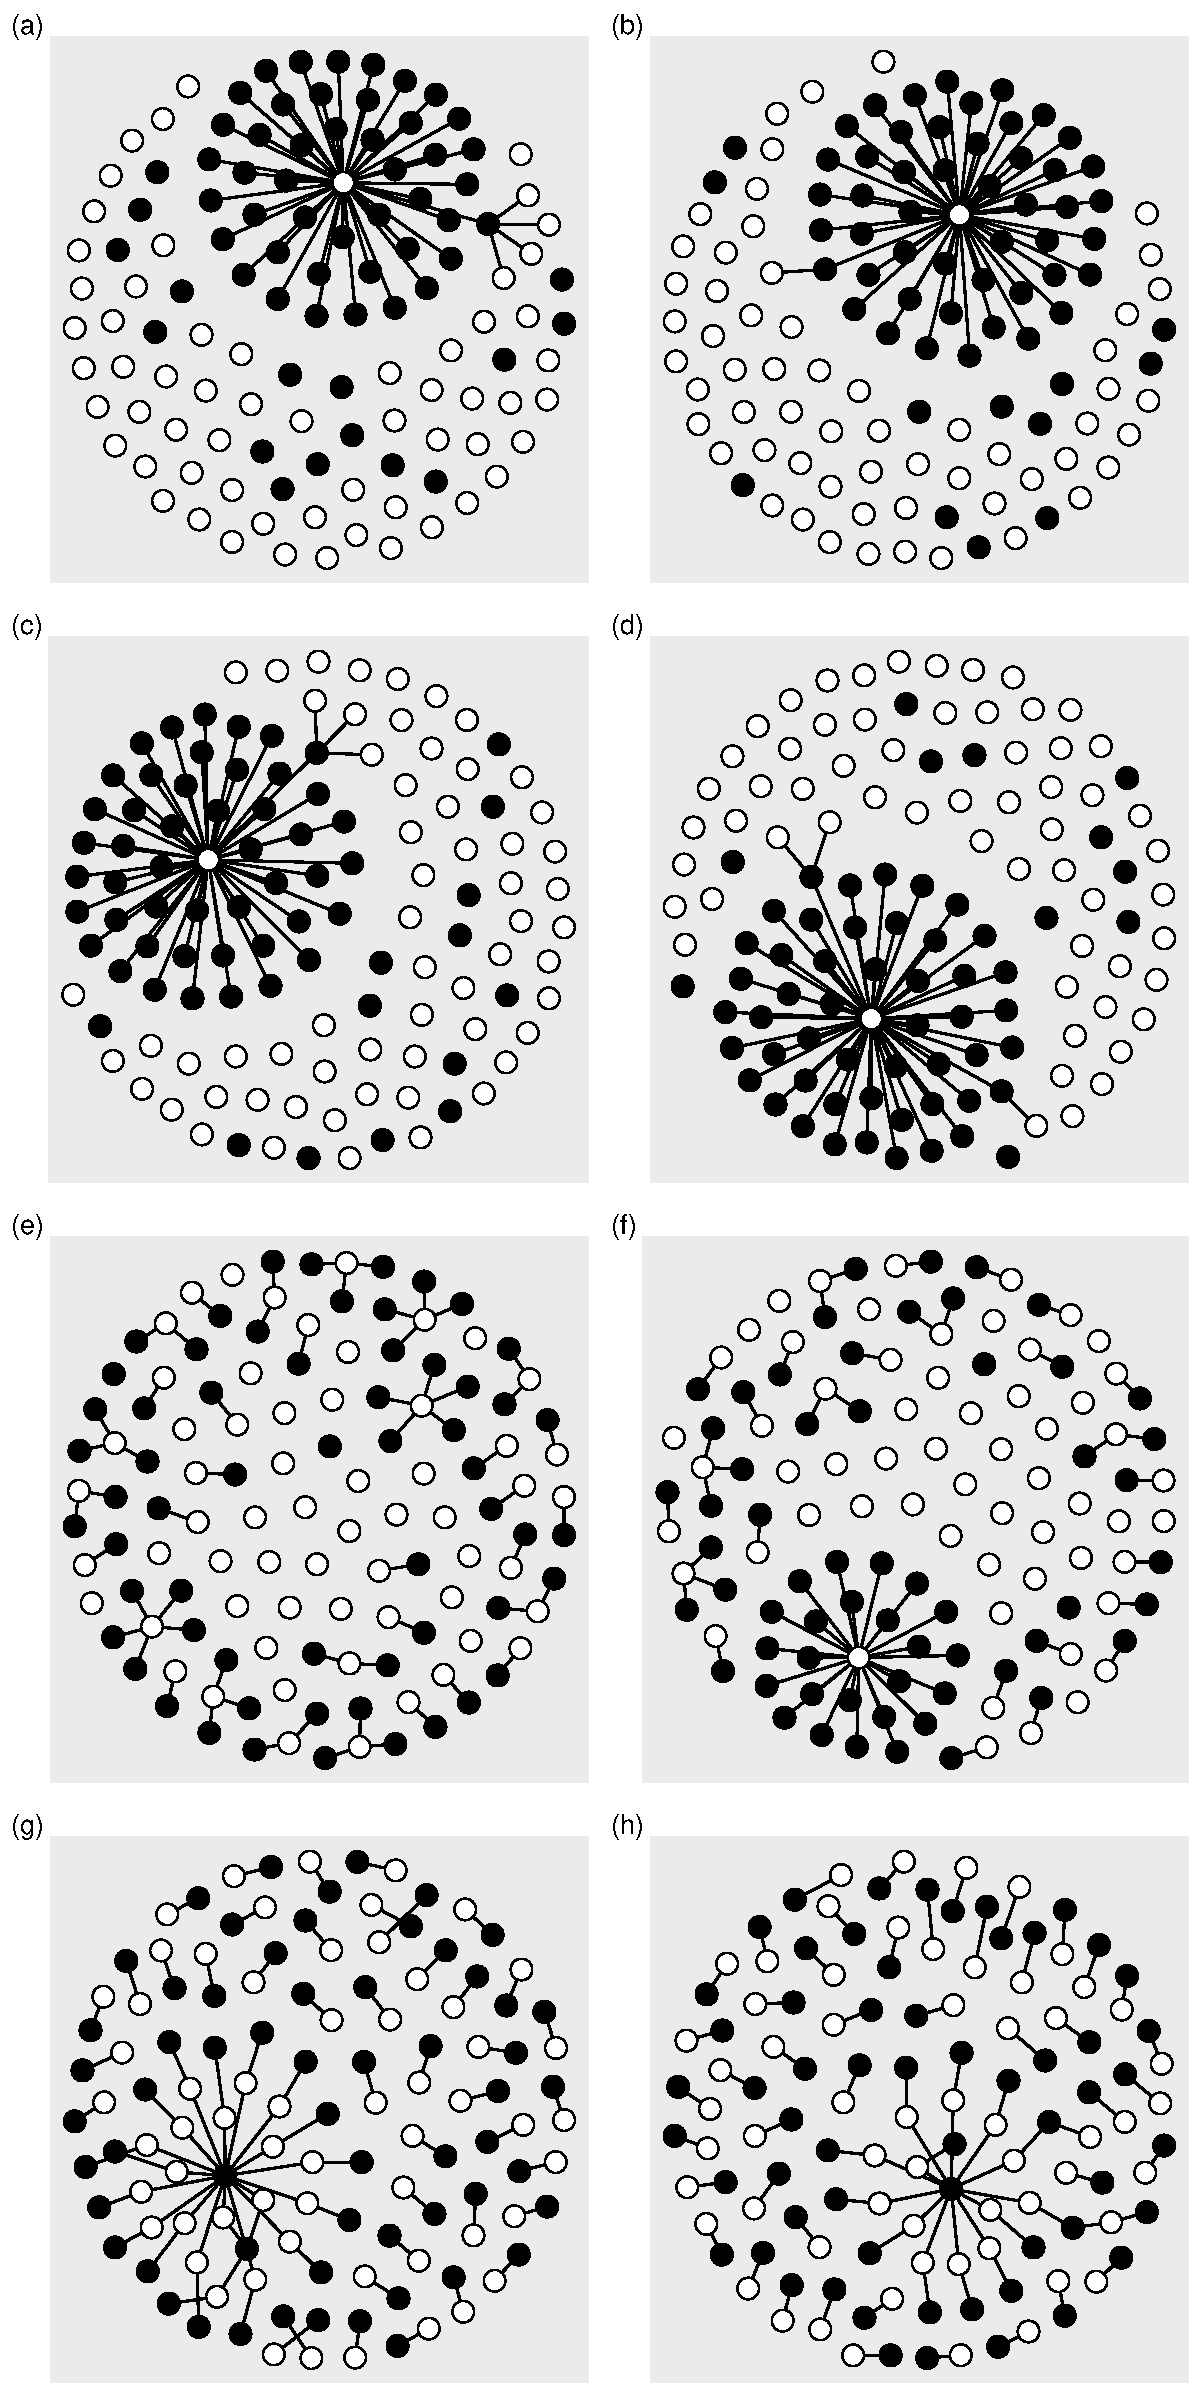
\includegraphics[height=\textheight,width=\textwidth,keepaspectratio]{graphVisualization_uniform_phi1_nm60_static_randomBipartite_allowUnlinked}
  \caption{a}
  \label{fig:graphVisualization_uniform_phi1_nm60_static_randomBipartite_allowUnlinked}
\end{figure}

\begin{figure}
  \centering
  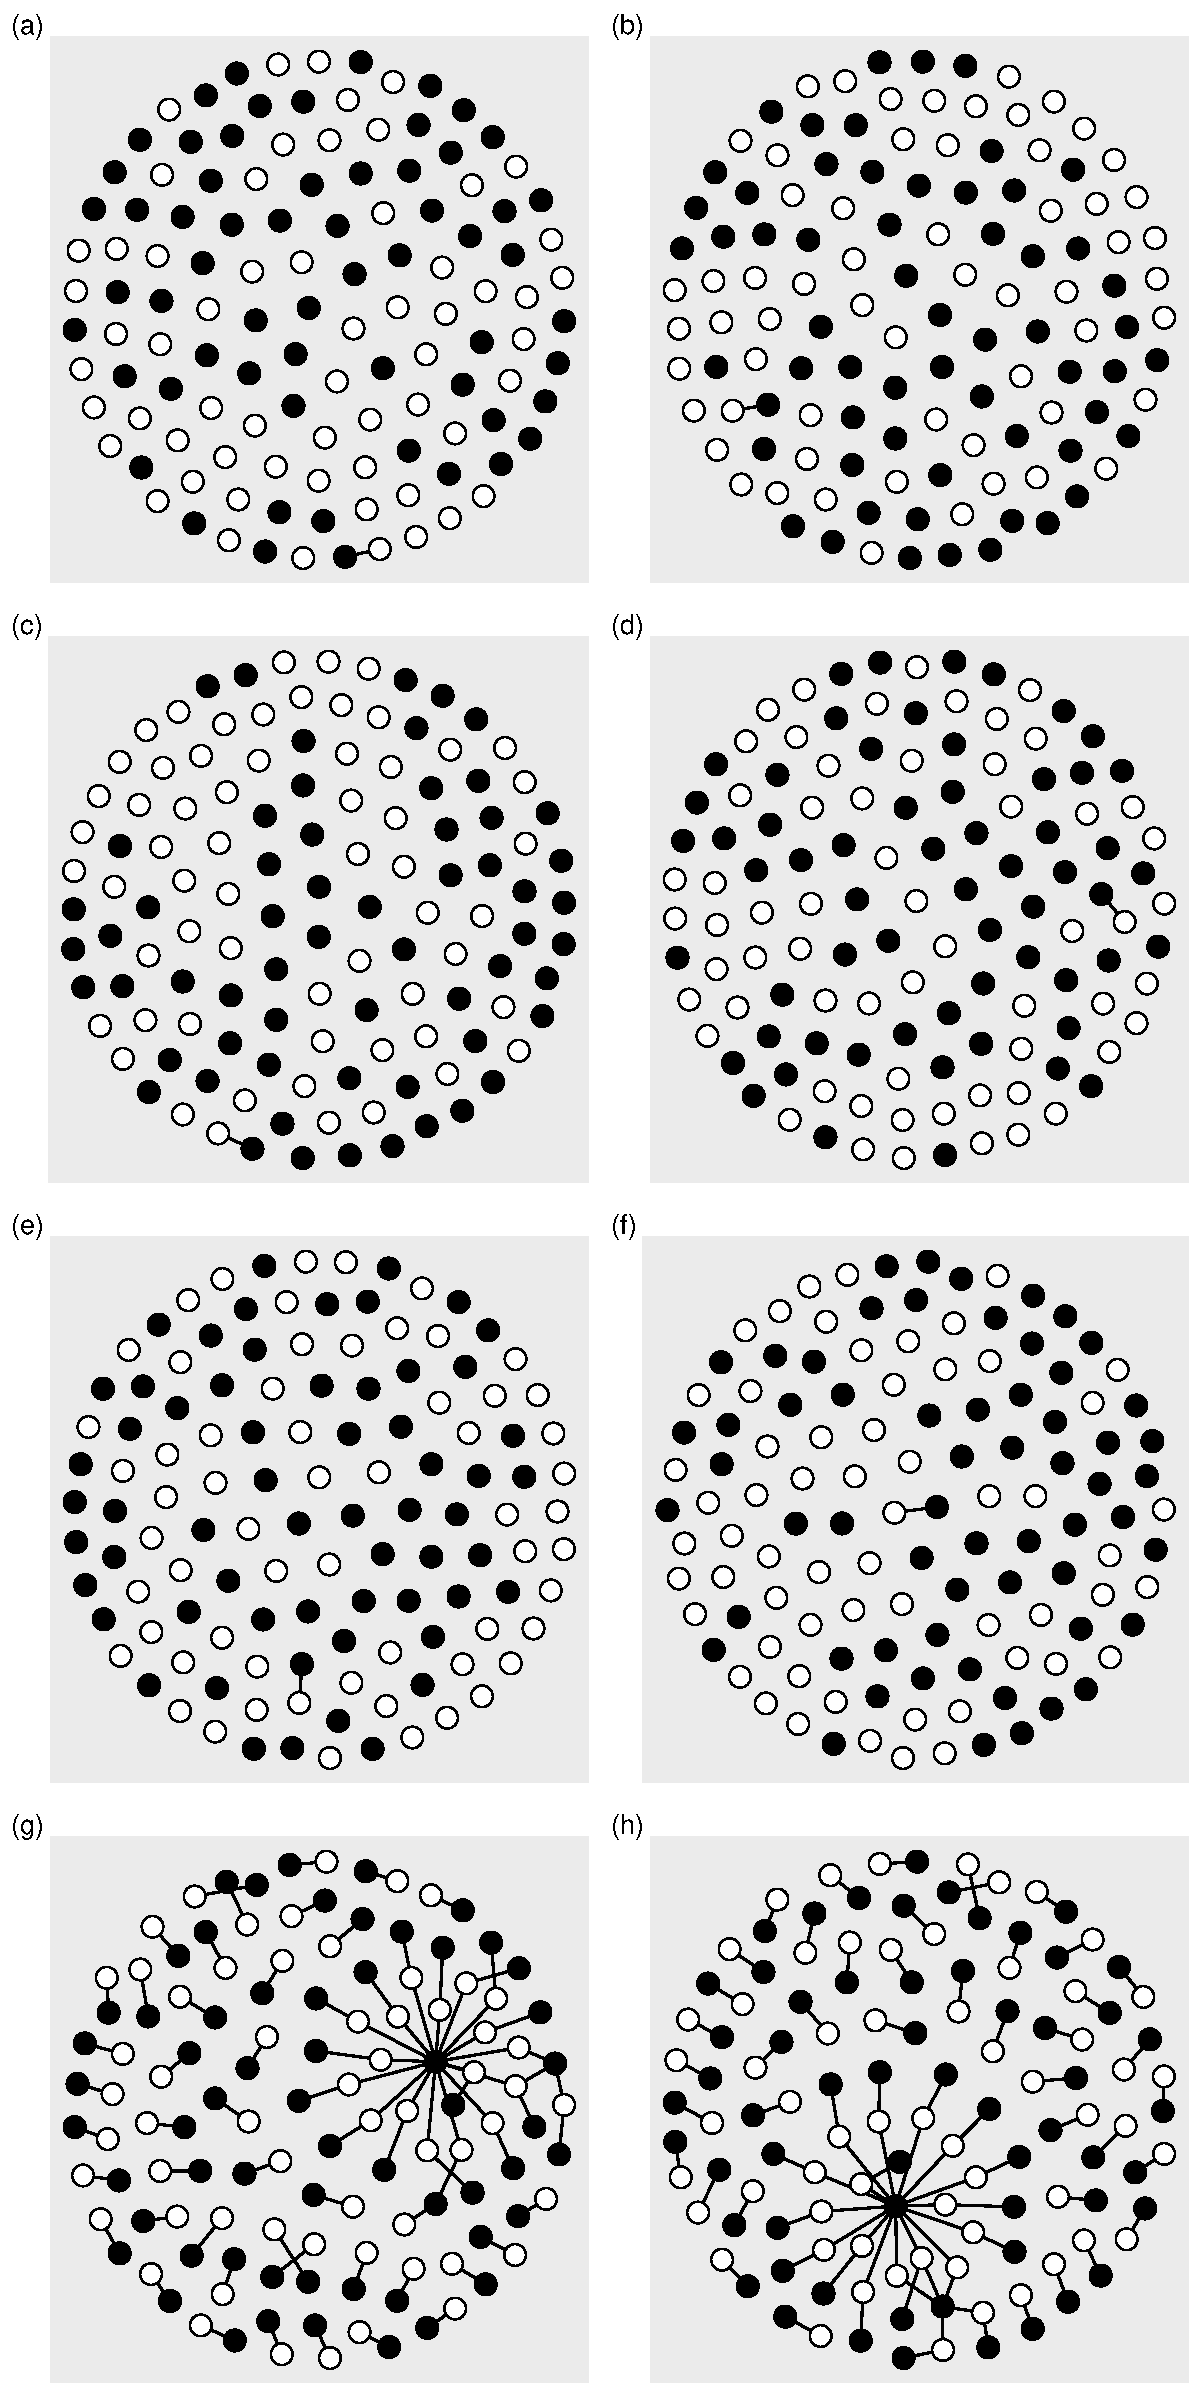
\includegraphics[height=\textheight,width=\textwidth,keepaspectratio]{graphVisualization_uniform_phi1_nm60_static_singleLink_allowUnlinked}
  \caption{a}
  \label{fig:graphVisualization_uniform_phi1_nm60_static_singleLink_allowUnlinked}
\end{figure}

\begin{figure}
  \centering
  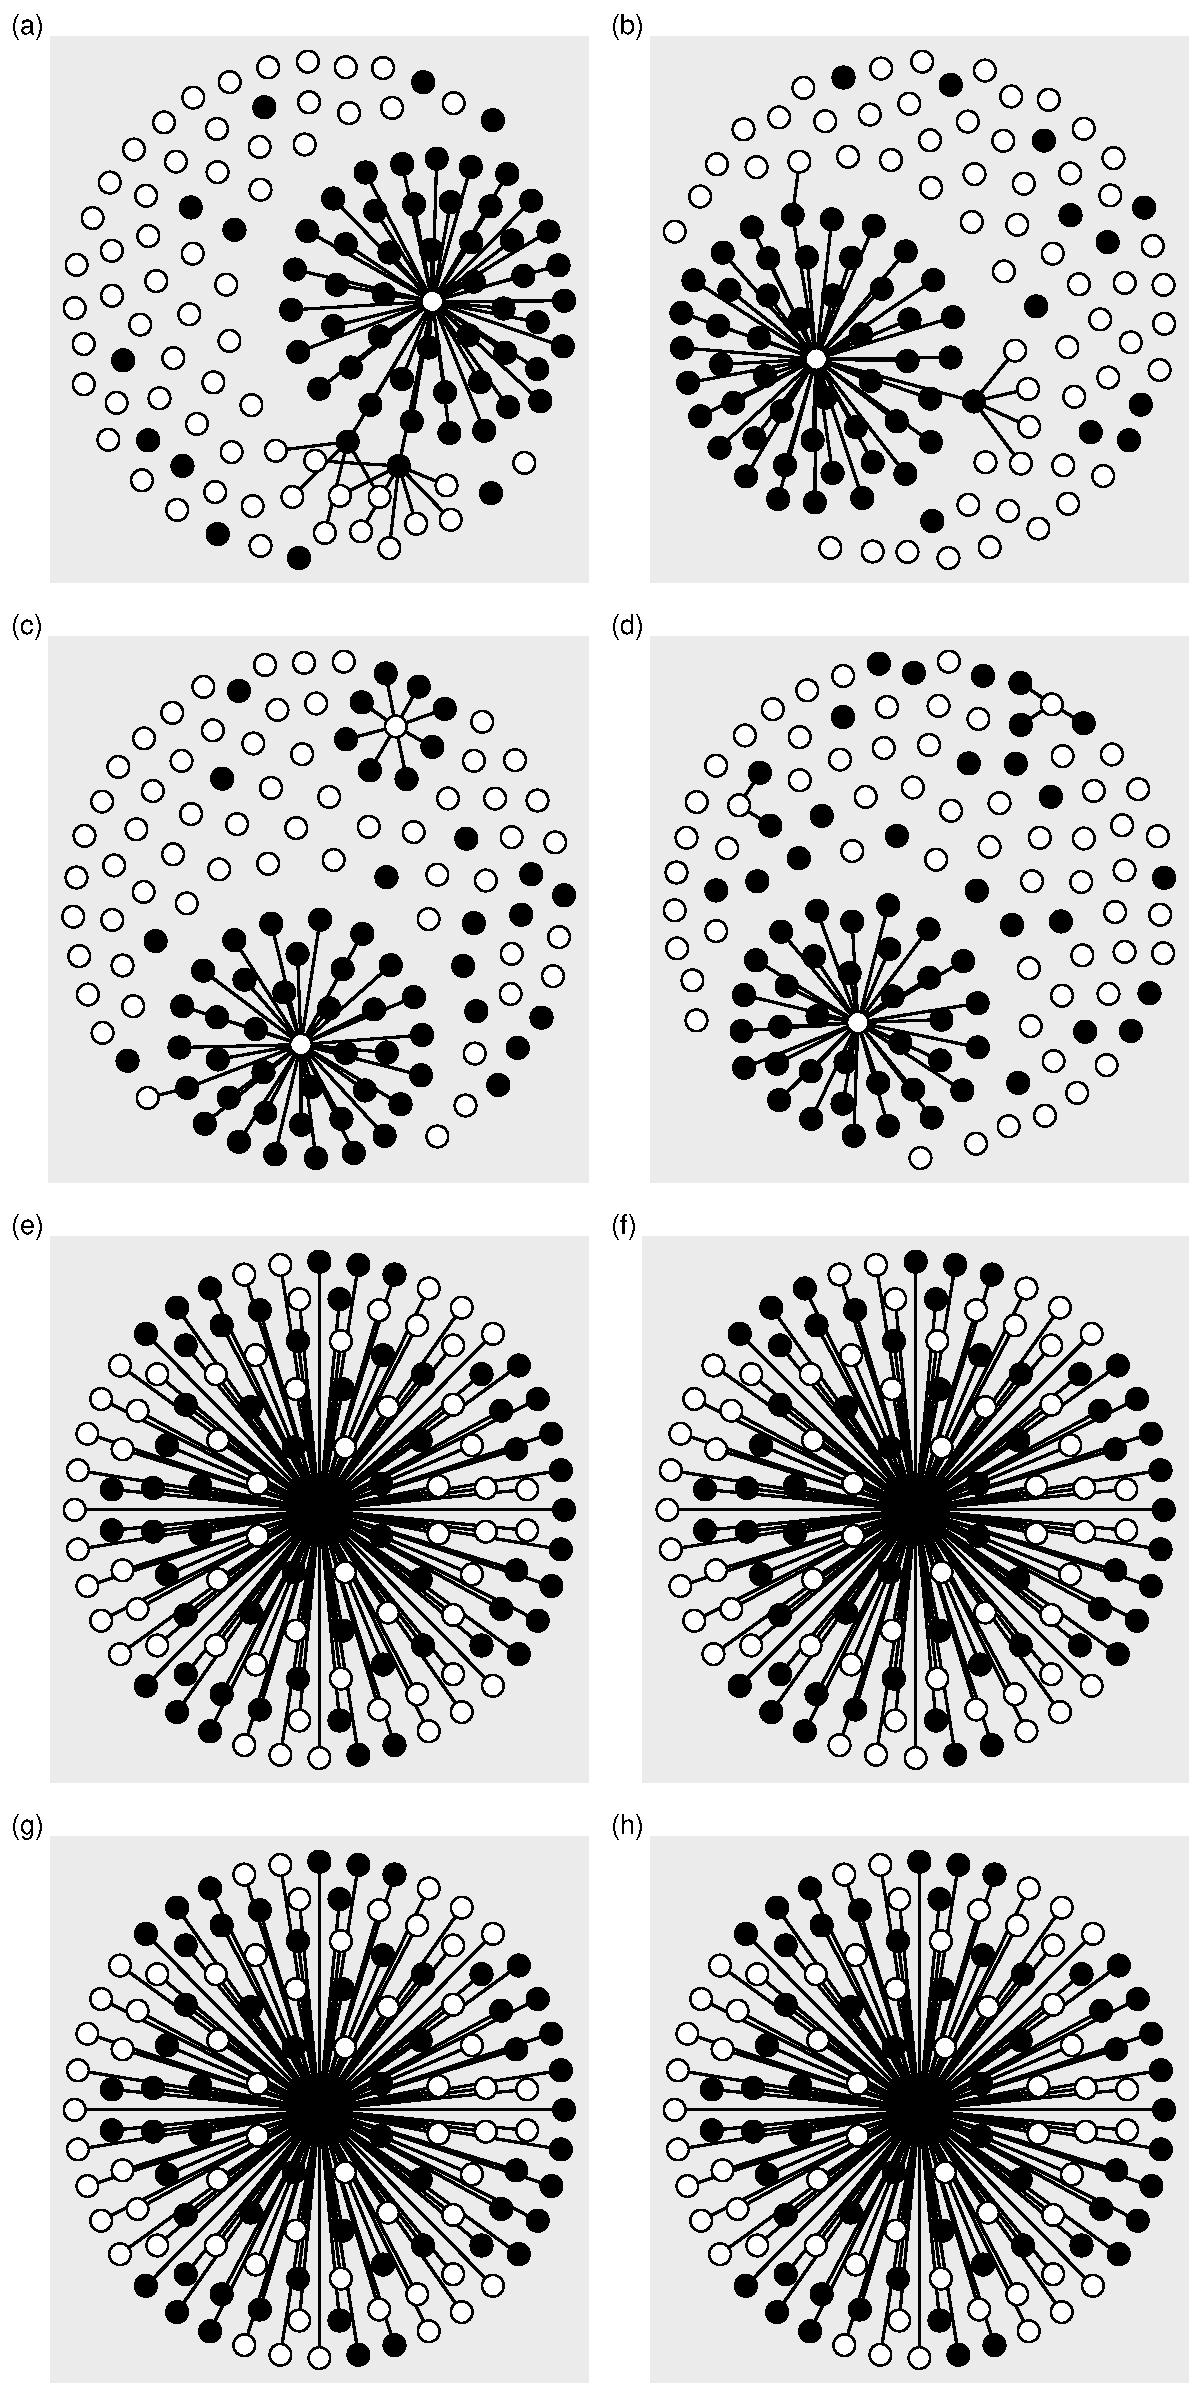
\includegraphics[height=\textheight,width=\textwidth,keepaspectratio]{graphVisualization_uniform_phi1_nm60_static_oneToOne_allowUnlinked}
  \caption{a}
  \label{fig:graphVisualization_uniform_phi1_nm60_static_oneToOne_allowUnlinked}
\end{figure}

\begin{figure}
  \centering
  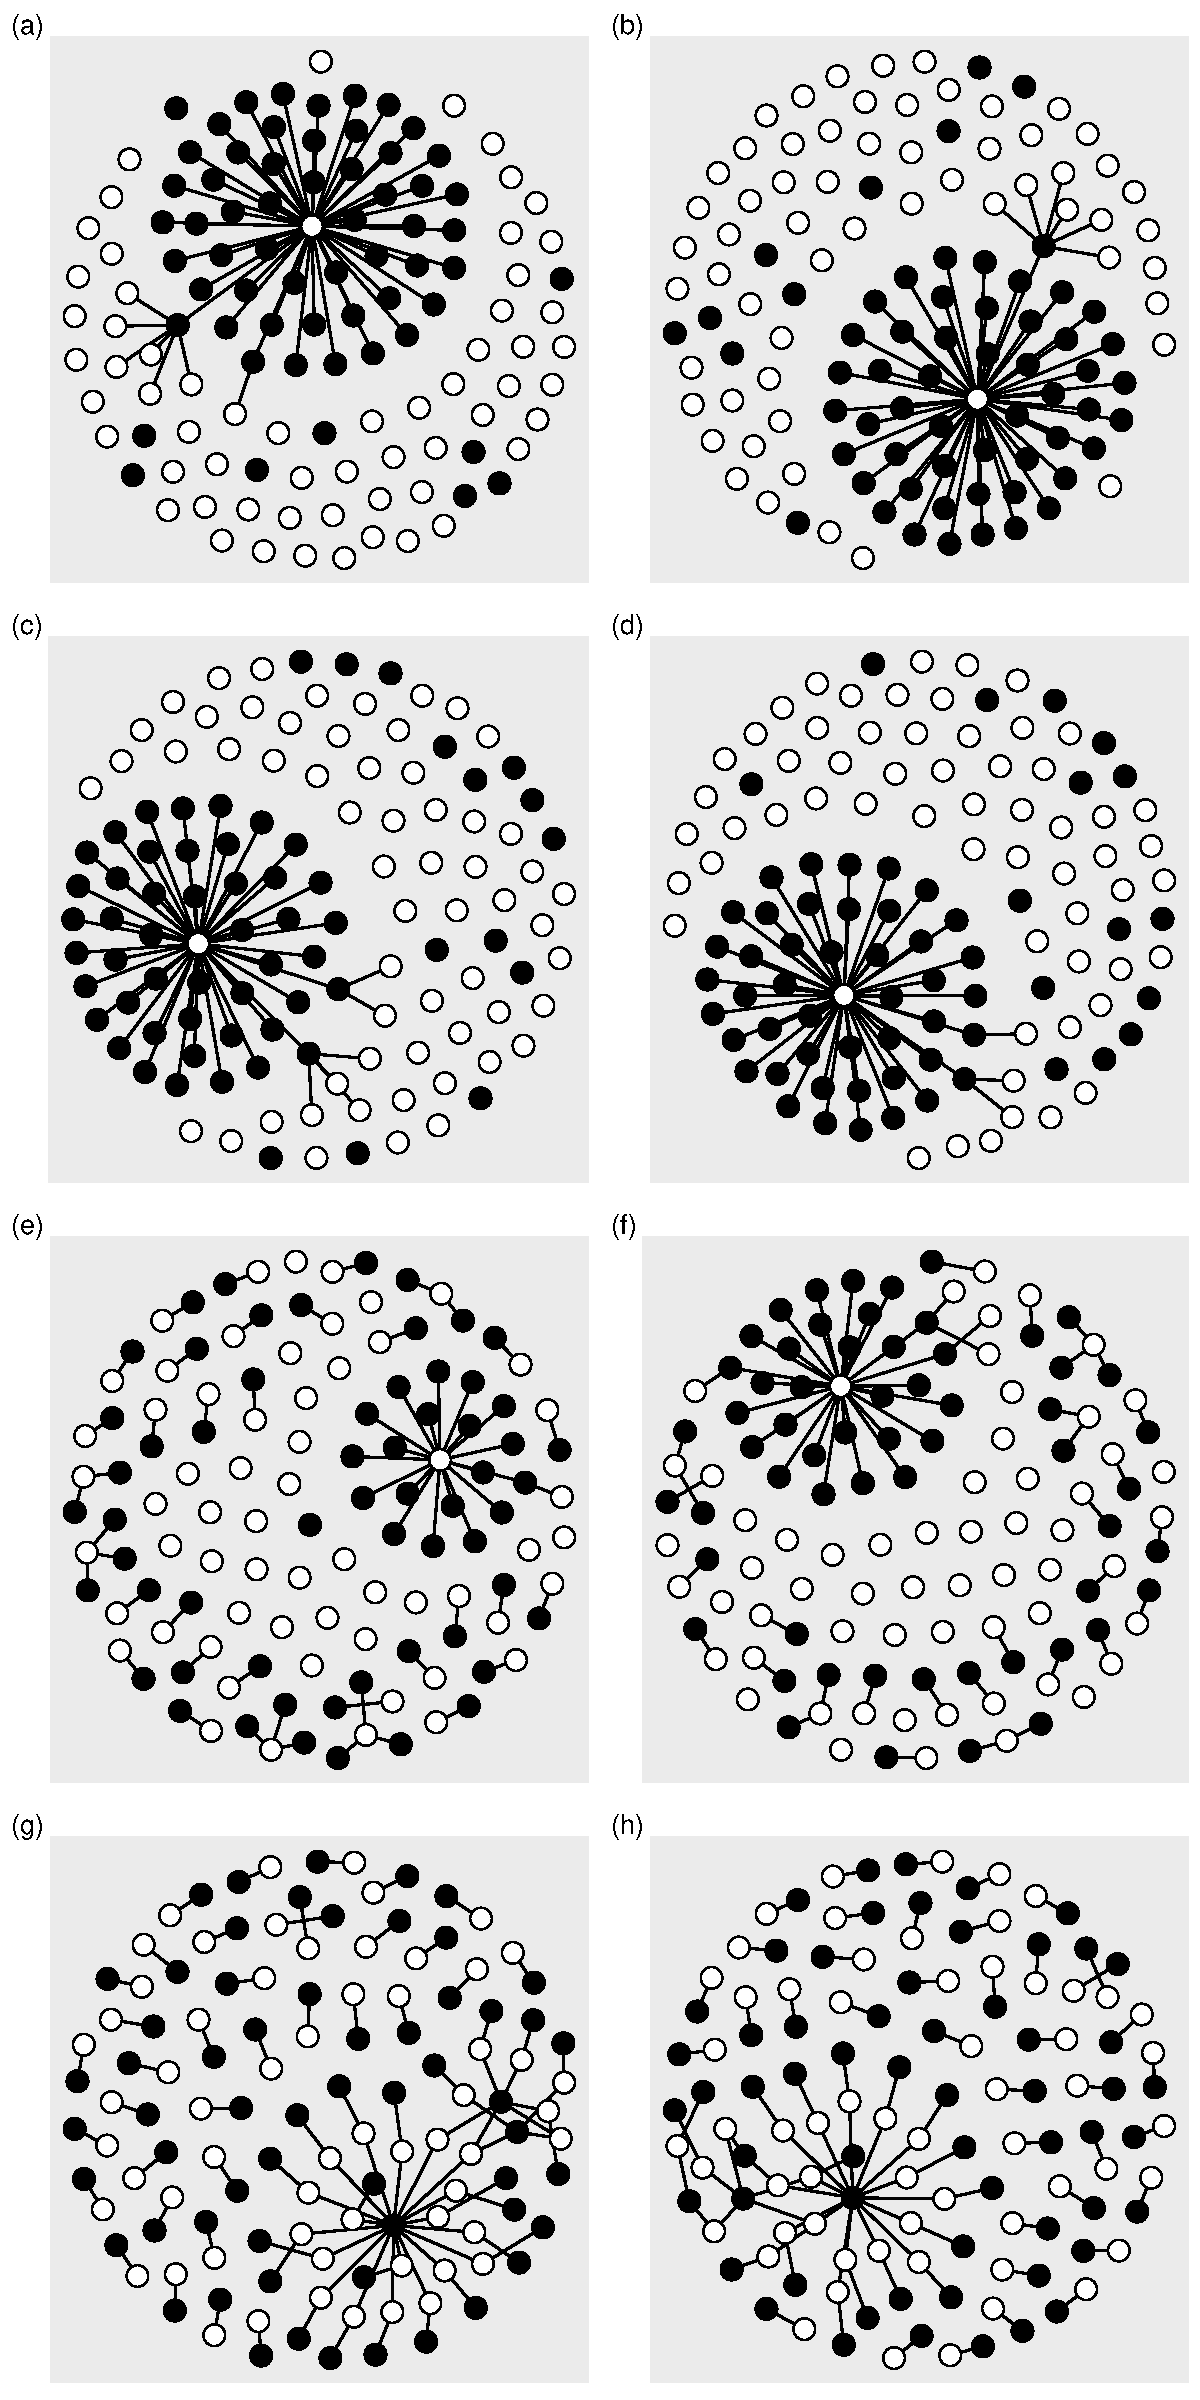
\includegraphics[height=\textheight,width=\textwidth,keepaspectratio]{graphVisualization_uniform_phi1_nm60_static_complete_allowUnlinked}
  \caption{a}
  \label{fig:graphVisualization_uniform_phi1_nm60_static_complete_allowUnlinked}
\end{figure}


\subsection{Information theoretic and statistical measures}
\label{sec:results_new_other}

This section shows the data obtained from executing simulations with various sets of parameters.
All simulations are run with a graph size of $n=m=400$.
Every experiment in this section is the result of averaging at least 20 realizations.
Most experiments consist of 100 realizations.
Some had to be reduced to 20 realizations due to the total running time and are marked as such.
Results for $\phi=0$ and $\phi=1$ are shown.
Three different initial conditions are tested: random bipartite graph, single link and one-to-one.
For the \secondmodel{} only results for $\pi$ following a uniform probability distribution are shown.
The chosen $\lambda$ value for which curves are fitted is the one that's qualitatively closer to a power law.

For the \firstmodel{} with $\phi=0$, Figures \ref{fig:informationTheoretic_firstModel_phi0_nm400_dynamic_randomBipartite_allowUnlinked}, \ref{fig:informationTheoretic_firstModel_phi0_nm400_dynamic_singleLink_allowUnlinked} and \ref{fig:informationTheoretic_firstModel_phi0_nm400_dynamic_oneToOne_allowUnlinked} show the information theoretic measures of the optimal graph for values of $\lambda$ ranging from 0 to 1.
They correspond to the random graph, single link and one-to-one initial graphs respectively. It can be seen how there is a phase transition when $\lambda \approx 0.5$.
There is a change in the behavior before the point where the phase changes in both the random bipartite and the one-to-one initial conditions but not in the single link.

\begin{figure}
  \centering
  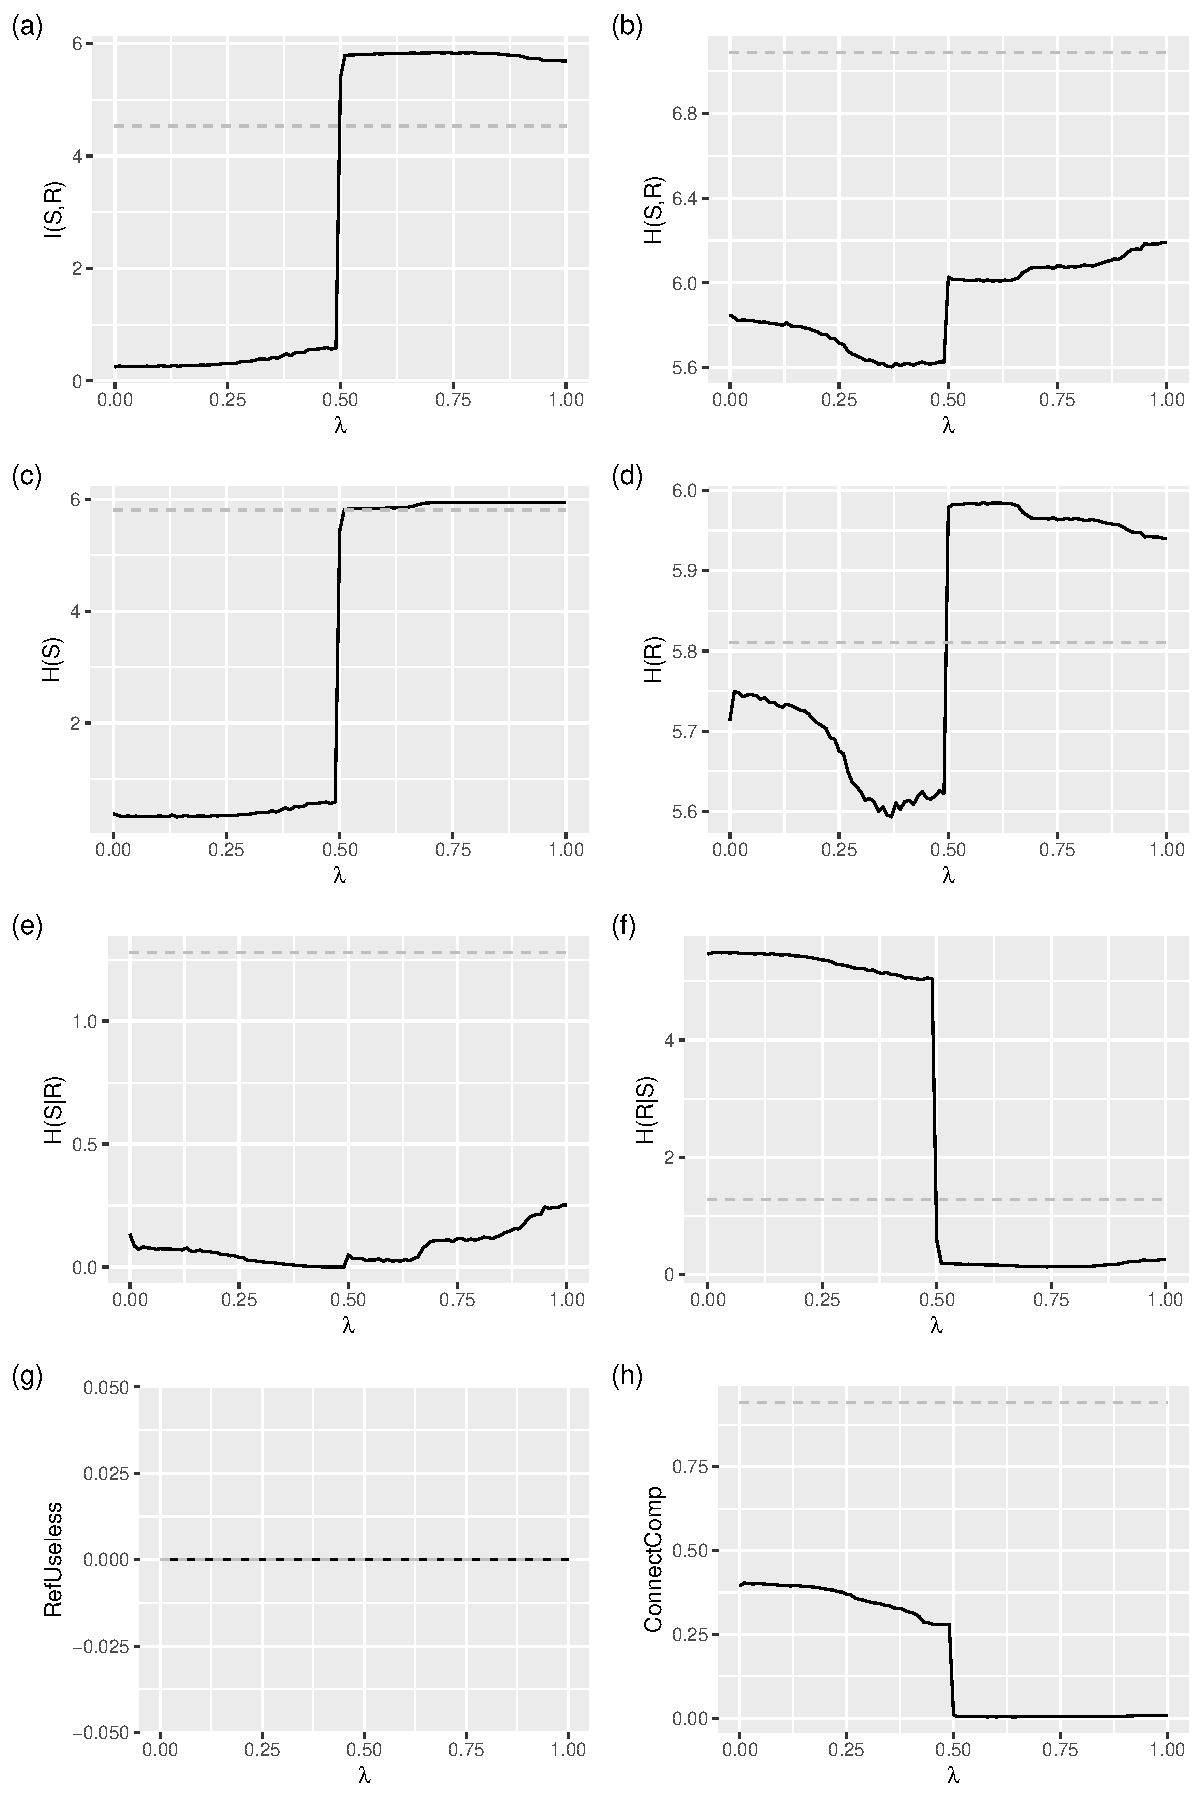
\includegraphics[height=0.7\textheight]{informationTheoretic_firstModel_phi0_nm400_dynamic_randomBipartite_allowUnlinked}
  \caption{
    Information theoretic measures for the optimized graph.
    The graph follows the equations of the \firstmodel{} with $\phi=0$ and the initial condition of the optimization process is a random bipartite graph \randgraph{n}{m}{\frac{3}{nm}}. Disconnected meanings are allowed.
    On the $x$ axis of each subfigure is the parameter $\lambda$ of the optimization process, ranging from 0 to 1.
    On the $y$ of the subfigures is: the mutual information between words and meanings (a), the joint entropy between words and meanings (b), the entropy of words (c), the entropy of meanings (d), the conditional entropy of words given the meanings (e), the conditional entropy of the meanings given the words (f), the number of referentially useless words (g) and the proportion of the largest connected component of the graph (h).
    A word $s_i$ is referentially useless if it is connected to at least one meaning and for each meaning $r_j$ it is connected to, $p(s_i,r_j) \leq p(s_i) \cdot p(r_j)$.
    Averages over 100 realizations.
}
  \label{fig:informationTheoretic_firstModel_phi0_nm400_dynamic_randomBipartite_allowUnlinked}
\end{figure}

\begin{figure}
  \centering
  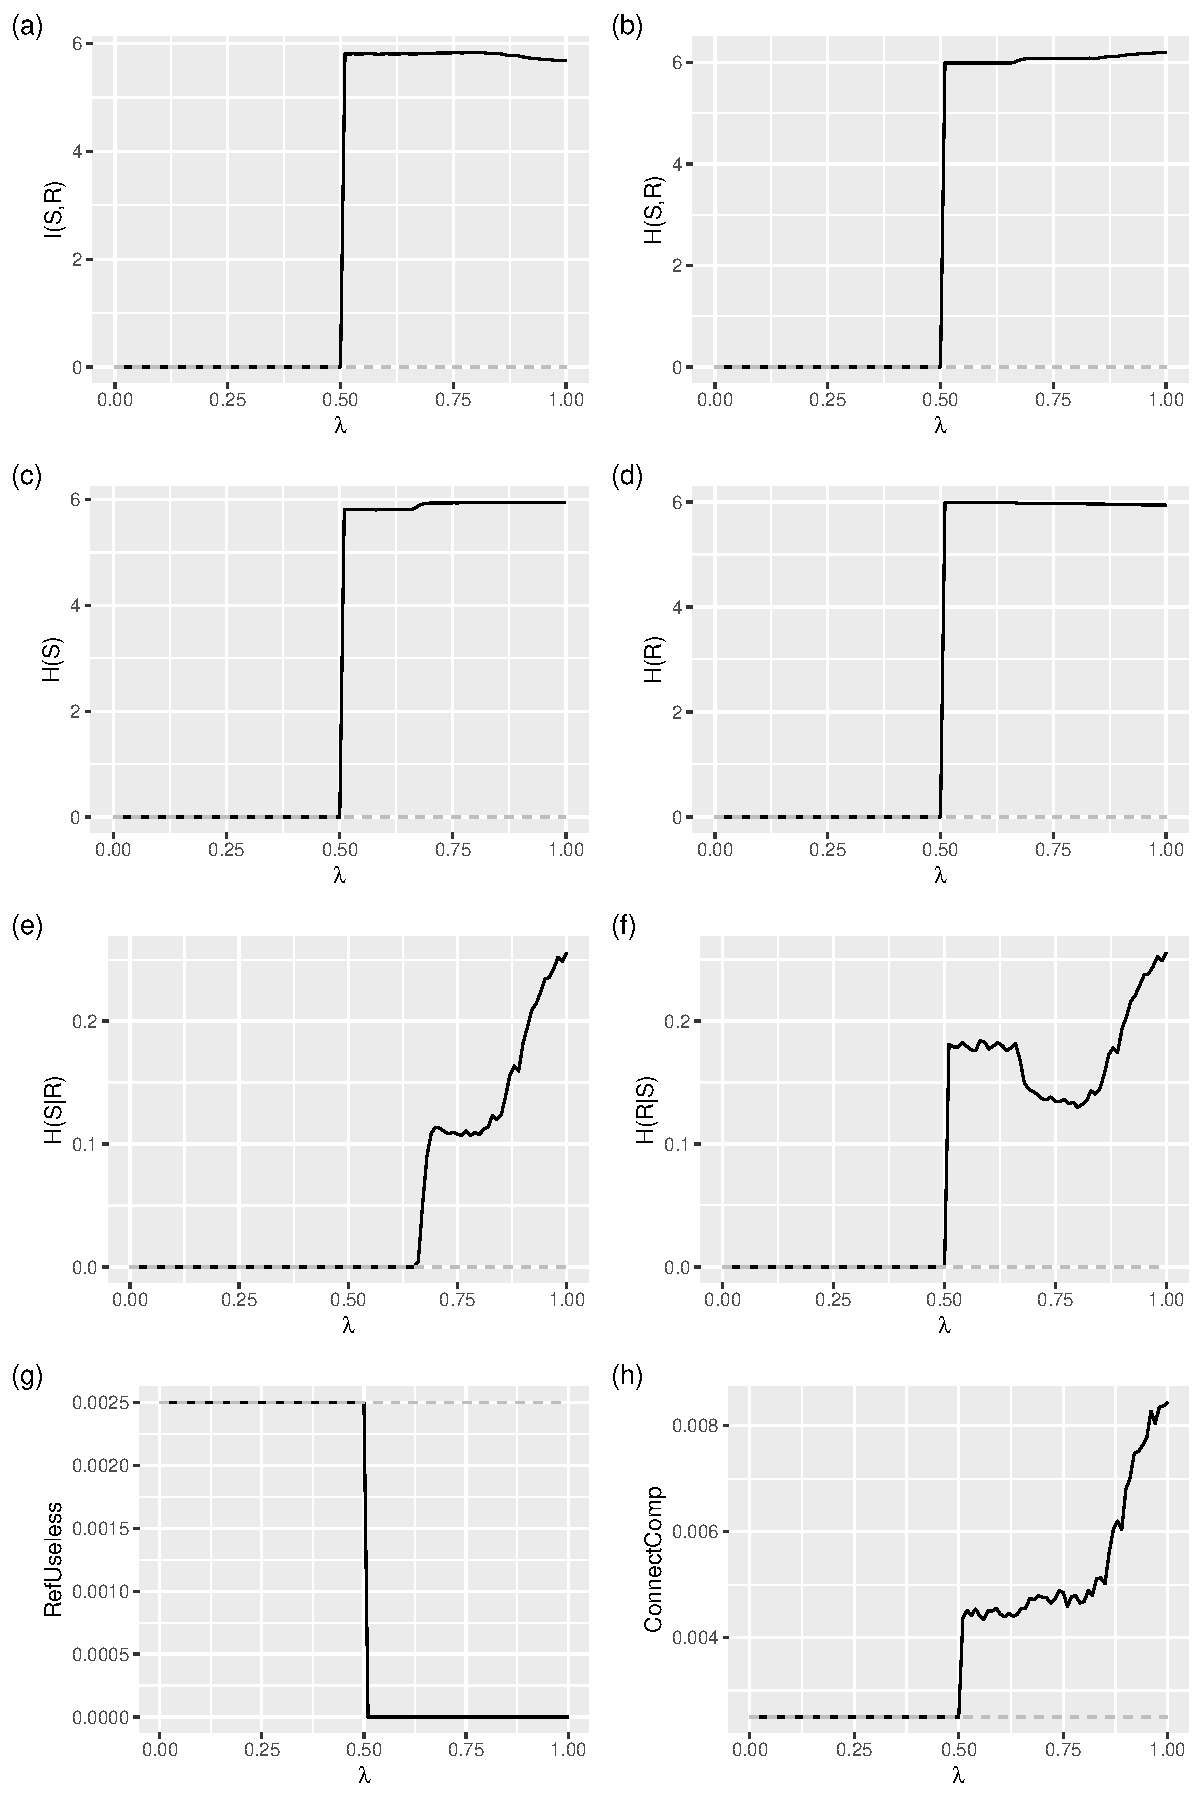
\includegraphics[height=0.7\textheight]{informationTheoretic_firstModel_phi0_nm400_dynamic_singleLink_allowUnlinked}
  \caption{Same information as in Figure \ref{fig:informationTheoretic_firstModel_phi0_nm400_dynamic_randomBipartite_allowUnlinked} but for a single link as the initial condition.}
  \label{fig:informationTheoretic_firstModel_phi0_nm400_dynamic_singleLink_allowUnlinked}
\end{figure}

\begin{figure}
  \centering
  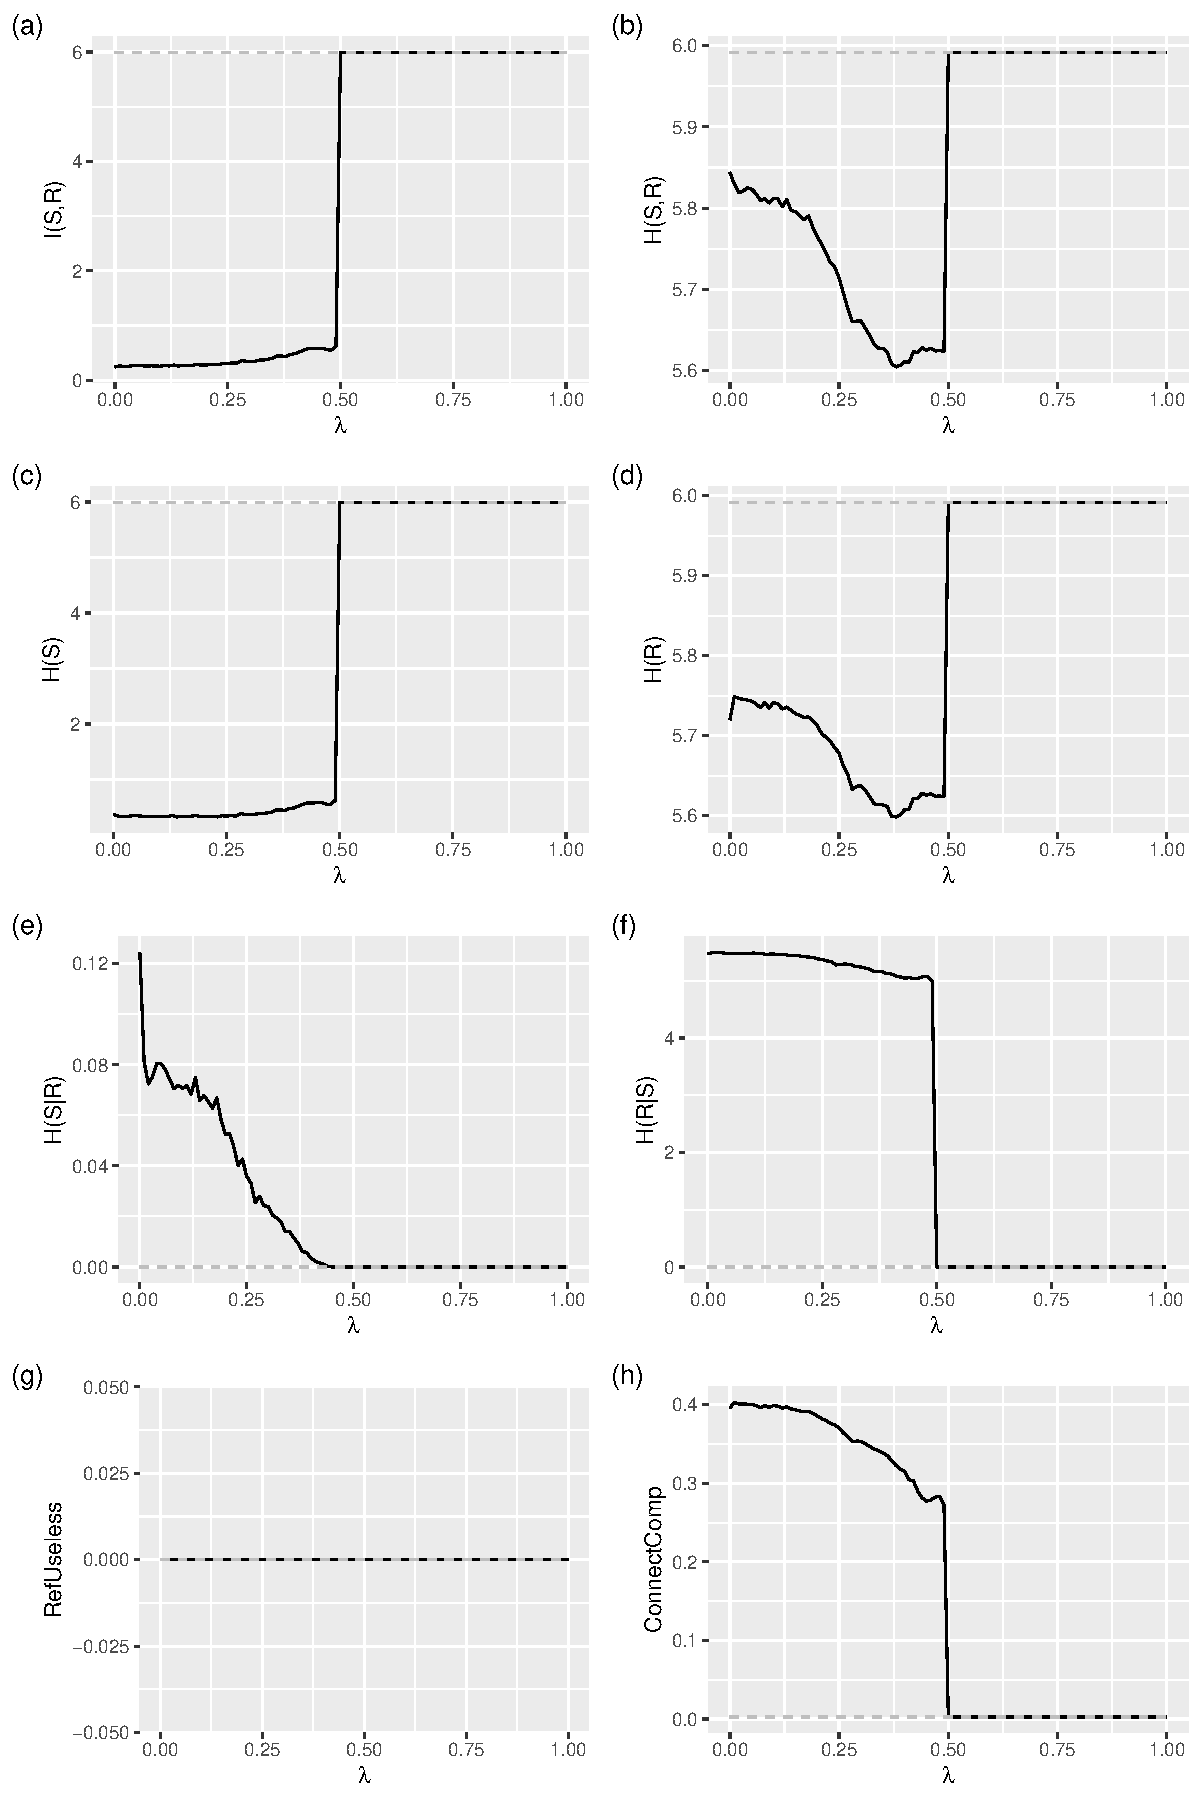
\includegraphics[height=0.7\textheight]{informationTheoretic_firstModel_phi0_nm400_dynamic_oneToOne_allowUnlinked}
  \caption{Same information as in Figure \ref{fig:informationTheoretic_firstModel_phi0_nm400_dynamic_randomBipartite_allowUnlinked} but for one to one connections between signals and meanings as the initial condition.}
  \label{fig:informationTheoretic_firstModel_phi0_nm400_dynamic_oneToOne_allowUnlinked}
\end{figure}

Figures \ref{fig:insideLambda_firstModel_phi0_nm400_dynamic_randomBipartite_allowUnlinked} and \ref{fig:insideLambda_firstModel_phi0_nm400_dynamic_oneToOne_allowUnlinked} (random and one-to-one initial conditions respectively) show statistical measures of select values of $\lambda$, with Figures \ref{fig:fitting_insideLambda_firstModel_phi0_nm400_dynamic_randomBipartite_allowUnlinked} and \ref{fig:fitting_insideLambda_firstModel_phi0_nm400_dynamic_oneToOne_allowUnlinked} (random and one-to-one respectively) showing the fitting of the curve to a power law for a single select value of $\lambda$.
It can be seen that a power law (linear in log-log scale) appears in the plots.
Tables \ref{tab:fitting_insideLambda_firstModel_phi0_nm400_dynamic_randomBipartite_allowUnlinked} and \ref{tab:fitting_insideLambda_firstModel_phi0_nm400_dynamic_oneToOne_allowUnlinked} (random and one-to-one respectively) showing the values of the regression exponent and factor.
The single link initial condition is not plotted for select values of $\lambda$ as it fails to evolve beyond the single link state.

\begin{figure}
  \centering
  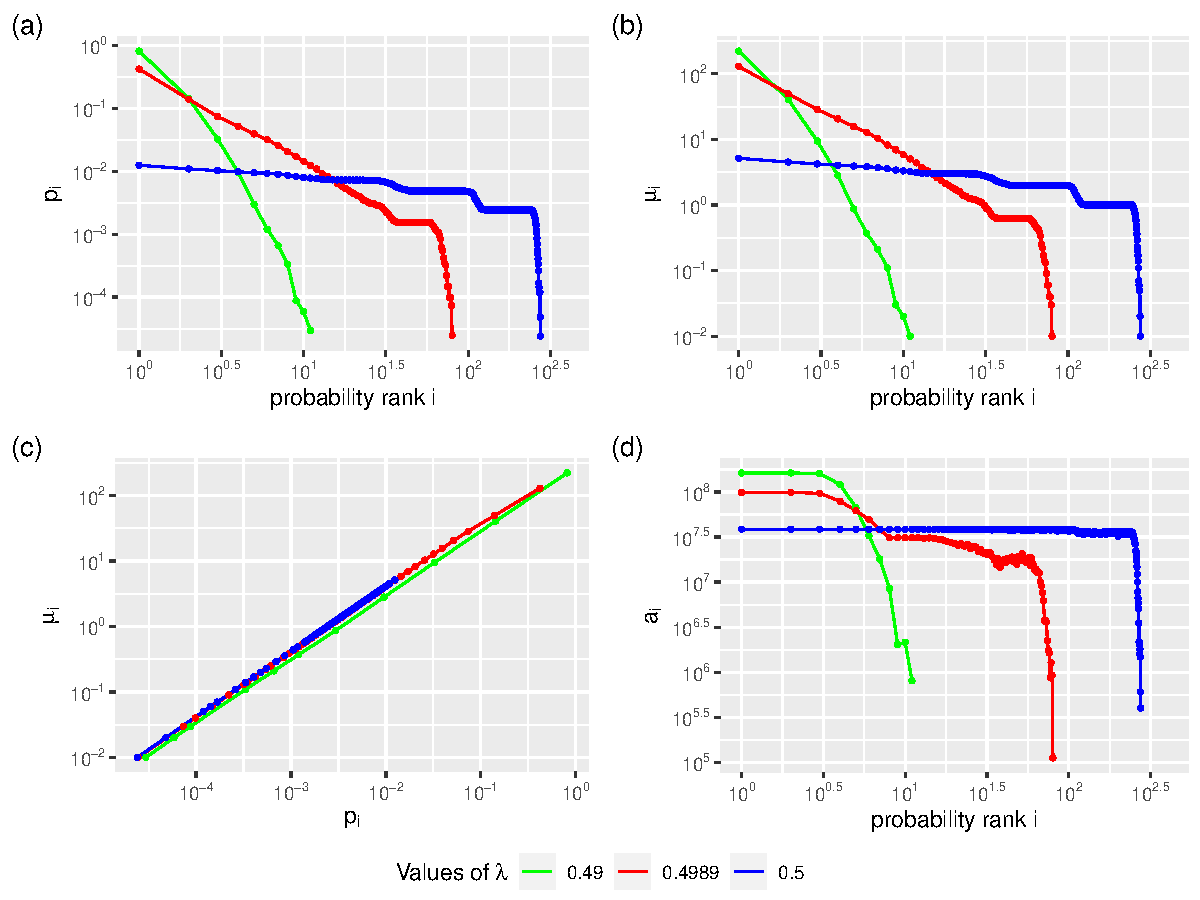
\includegraphics[height=0.7\textheight]{insideLambda_firstModel_phi0_nm400_dynamic_randomBipartite_allowUnlinked}
  \caption{
    Statistical measures of the optimized graph for select values of $\lambda$.
    The graph follows the equations of the \firstmodel{} with $\phi=0$ and the initial condition of the optimization process is a random bipartite graph \randgraph{n}{m}{\frac{3}{nm}}. Disconnected meanings are allowed.
    The green line corresponds to $\lambda=0.49$, the blue line to $\lambda=0.5$ and the red line to $\lambda=\lambda^*$.
    The value of $\lambda^*$ is chosen qualitatively and in this case $\lambda^*=0.4989$.
    Figure (a) shows the probability (or frequency) of a word as a function of its probability rank.
    Figure (b) shows the cumulative proportion of the frequency of words.
    Figure (c) shows the number of meanings of a word as a function of its probability rank.
    Figure (d) shows the number of meanings of a word as a function of its probability.
    Figure (e) shows age of a word as a function of its probability rank.
    Figure (f) shows the number of meanings of a word as a function of its degree rank.
    Figure (g) shows the cumulative proportion of the number of meanings of words.
    All figures are in a log-log scale.
    Averages over 100 realizations.
  }
  \label{fig:insideLambda_firstModel_phi0_nm400_dynamic_randomBipartite_allowUnlinked}
\end{figure}

\begin{figure}
  \centering
  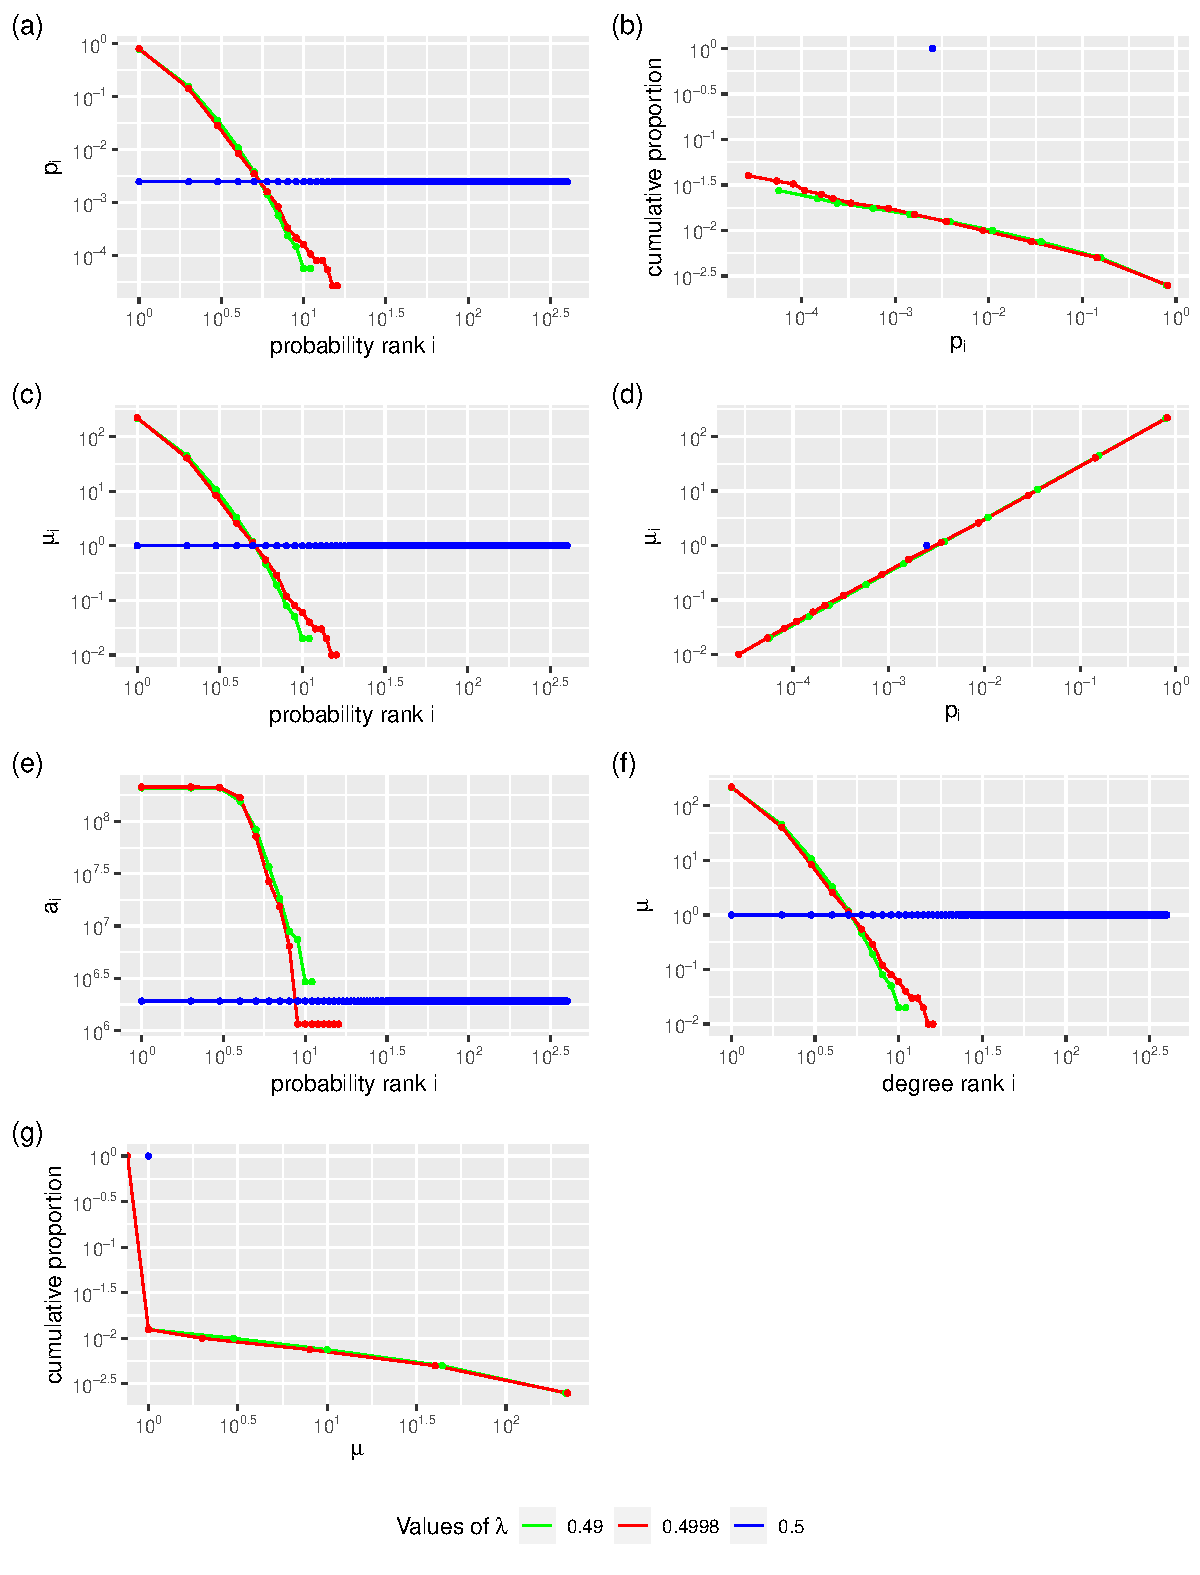
\includegraphics[height=0.7\textheight]{insideLambda_firstModel_phi0_nm400_dynamic_oneToOne_allowUnlinked}
  \caption{Same information as in Figure \ref{fig:insideLambda_firstModel_phi0_nm400_dynamic_randomBipartite_allowUnlinked} but the initial condition is one to one connections between words and meanings. $\lambda^* = 0.4989$}
  \label{fig:insideLambda_firstModel_phi0_nm400_dynamic_oneToOne_allowUnlinked}
\end{figure}

\begin{figure}
  \centering
  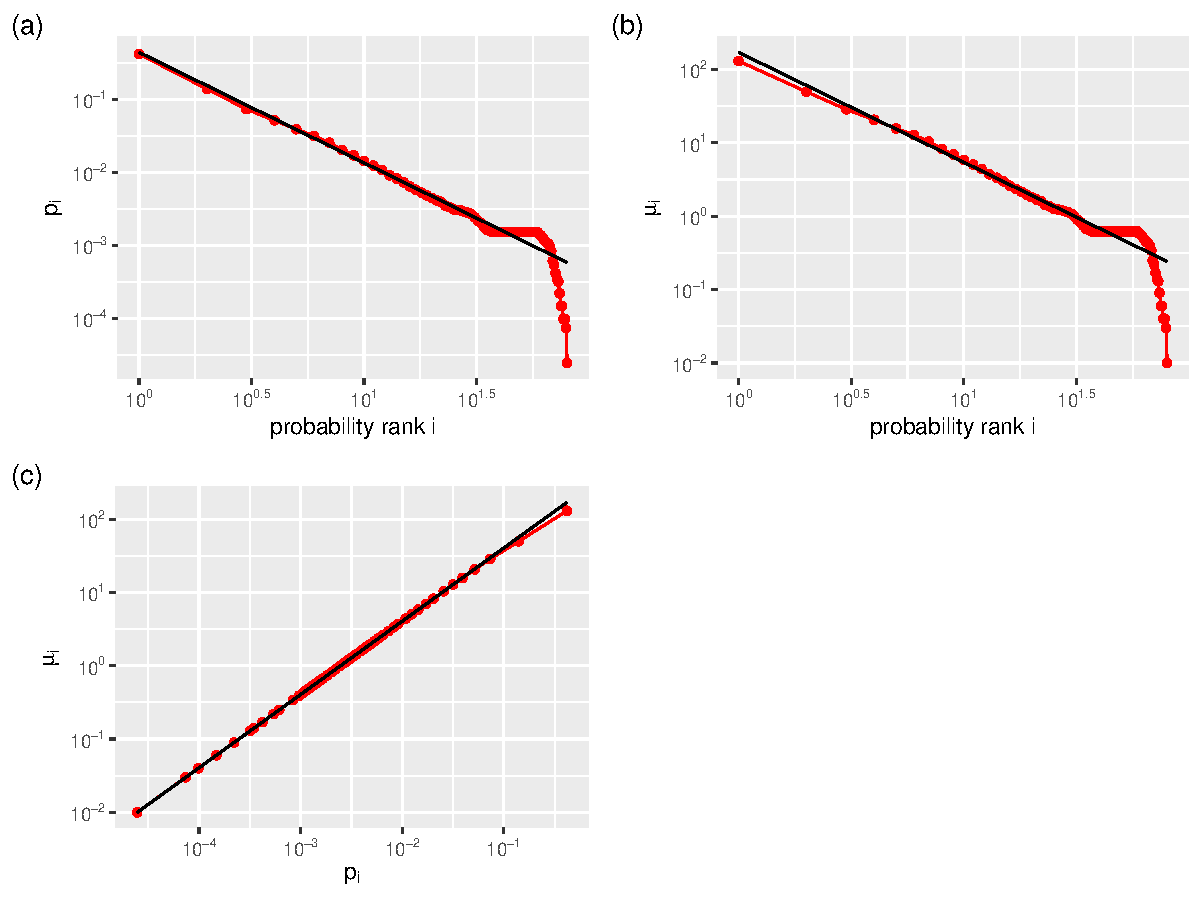
\includegraphics[height=0.65\textheight]{fitting_insideLambda_firstModel_phi0_nm400_dynamic_randomBipartite_allowUnlinked}
  \caption{
    Statistical measures of the optimized graph for a select value of $\lambda=\lambda^*$.
    The graph follows the equations of the \firstmodel{} with $\phi=0$ and the initial condition of the optimization process is a random bipartite graph \randgraph{n}{m}{\frac{3}{nm}}. Disconnected meanings are allowed.
    $\lambda^*=0.4989$.
    The black line indicates the values predicted by the Theil-Sen liniear regression.
    The red line indicates the actual values in the graph.
    Figure (a) shows the probability (or frequency) of a word as a function of its probability rank.
    Figure (b) shows the cumulative proportion of the frequency of words.
    Figure (c) shows the number of meanings of a word as a function of its probability rank.
    Figure (d) shows the number of meanings of a word as a function of its probability.
    Figure (f) shows the number of meanings of a word as a function of its degree rank.
    Figure (g) shows the cumulative proportion of the number of meanings of words.
    Figure (e), which should show the age of a word as a function of its probability rank, is omitted as it never followed a power law.
    All figures are in a log-log scale.
    Table \ref{tab:fitting_insideLambda_firstModel_phi0_nm400_dynamic_randomBipartite_allowUnlinked} shows the values of the exponent and the factor of the fitted power law.
  }
  \label{fig:fitting_insideLambda_firstModel_phi0_nm400_dynamic_randomBipartite_allowUnlinked}
\end{figure}

\begin{figure}
  \centering
  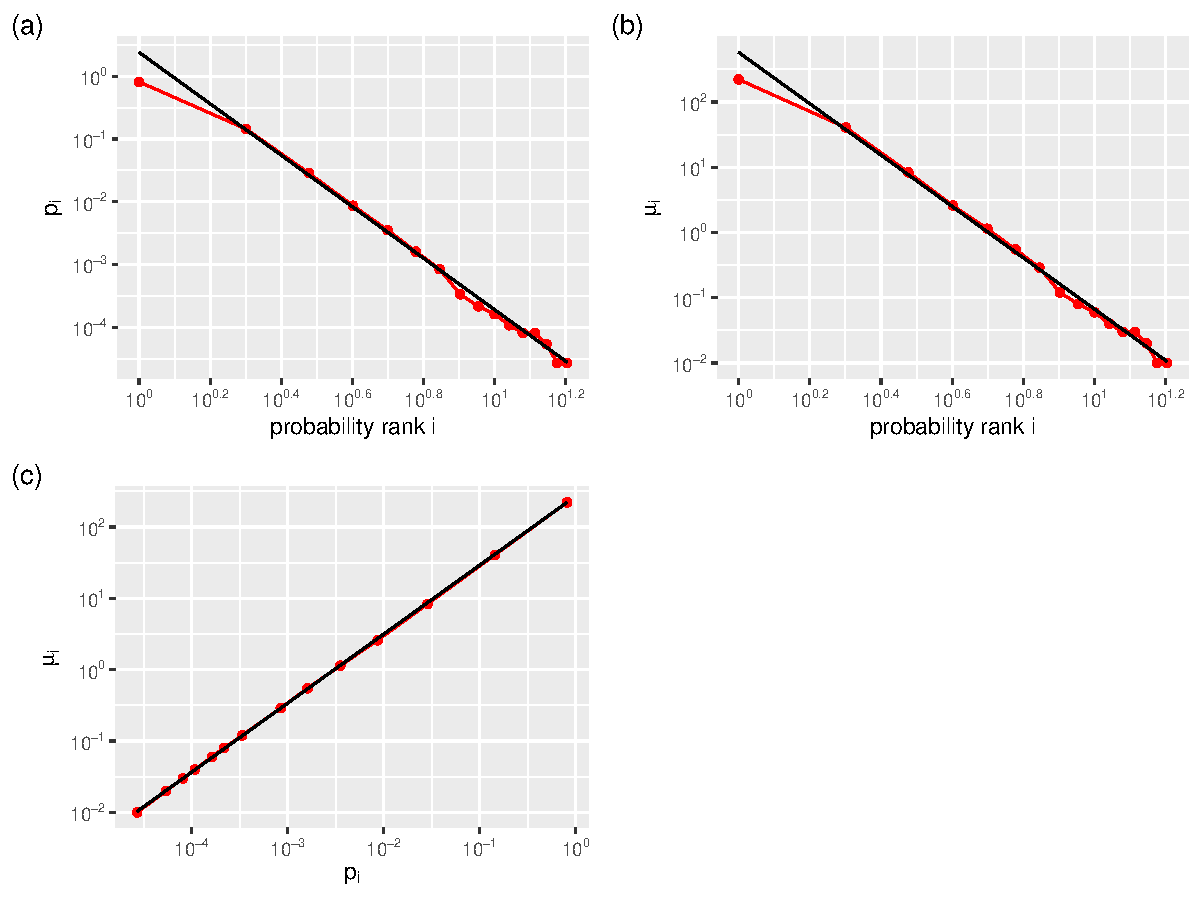
\includegraphics[width=\textwidth]{fitting_insideLambda_firstModel_phi0_nm400_dynamic_oneToOne_allowUnlinked}
  \caption{Same information as in Figure \ref{fig:fitting_insideLambda_firstModel_phi0_nm400_dynamic_randomBipartite_allowUnlinked} but the initial condition is one to one connections between words and meanings. $\lambda^*=0.
4989$.
Table \ref{tab:fitting_insideLambda_firstModel_phi0_nm400_dynamic_oneToOne_allowUnlinked} shows the values of the exponent and the factor of the fitted power law.}
  \label{fig:fitting_insideLambda_firstModel_phi0_nm400_dynamic_oneToOne_allowUnlinked}
\end{figure}

% latex table generated in R 4.0.4 by xtable 1.8-4 package
% Wed Mar 17 14:20:58 2021
\begin{table}
\centering
\begin{tabular}{lrr}
  \hline
plot & $\alpha$ & $k$ \\ 
  \hline
a & 1.5131590 & 0.4415009 \\ 
  b & 0.6406267 & 0.0016491 \\ 
  c & 1.4972982 & 170.7165580 \\ 
  d & -0.9992804 & 403.8279052 \\ 
  f & 1.4972982 & 170.7165580 \\ 
  g & 0.6725912 & 0.0750000 \\ 
   \hline
\end{tabular}
\caption{
  Table showing the exponent ($\alpha$) and the factor ($k$) of the power laws fitted in Figure \ref{fig:fitting_insideLambda_firstModel_phi0_nm400_dynamic_randomBipartite_allowUnlinked} for each of the subfigures. The power law follows the formula $y = kx^{-\alpha}$.
} 
\label{tab:fitting_insideLambda_firstModel_phi0_nm400_dynamic_randomBipartite_allowUnlinked}
\end{table}


\begin{table}
  \centering
  \begin{adjustbox}{max width=\textwidth}
    \begin{tabular}{llSS[scientific-notation=true]}
      \toprule
      plot & law & $a$ & $k$ \\ 
      \midrule
      a & word frequency ($\alpha$) & 4.0992847 & 2.3970141 \\ 
      %b & \redtxt{word frequency (cumulative)} & 0.2466051 & 0.0030639 \\ 
      b & meaning distribution ($\gamma$) & 3.9365300 & 577.6844467 \\ 
      c & meaning frequency ($\delta$) & -0.9673668 & 271.7315918 \\ 
      %f & \redtxt{meaning distribution} & 3.9365300 & 577.6844467 \\ 
      %g & \redtxt{meaning distribution (cumulative)} & 0.2731698 & 0.0125000 \\ 
      \bottomrule
    \end{tabular}
  \end{adjustbox}
  \caption{
    Table showing the exponent and factor of the power laws fitted for the \firstmodel{} with $\phi=0$ and a one to one configuration as the initial condition (Figure \ref{fig:fitting_insideLambda_firstModel_phi0_nm400_dynamic_oneToOne_allowUnlinked})
    In this table, $\alpha \approx 4$, $\delta \approx 1$ and $\gamma \approx 4$.
    The relationship between these values (Equation \eqref{eq:relation-exponents}) holds but the exponents are not exactly the ones expected.
  } 
  \label{tab:fitting_insideLambda_firstModel_phi0_nm400_dynamic_oneToOne_allowUnlinked}
\end{table}

%%% Local Variables:
%%% mode: latex
%%% TeX-master: "../tfm"
%%% End:



For the \firstmodel{} but $\phi=1$, Figures  \ref{fig:informationTheoretic_firstModel_phi1_nm400_dynamic_randomBipartite_allowUnlinked},  \ref{fig:informationTheoretic_firstModel_phi1_nm400_dynamic_singleLink_allowUnlinked} and  \ref{fig:informationTheoretic_firstModel_phi1_nm400_dynamic_oneToOne_allowUnlinked} show the information theoretic measures of the optimal graph for values of $\lambda$ ranging from 0 to 1.
They correspond to the random graph, single link and one-to-one initial graphs respectively.
As with the $\phi=0$ variant, there is a phase transition when $\lambda \approx 0.
5$.
The changes before that point, however, are much less pronounced.

\begin{figure}
  \centering
  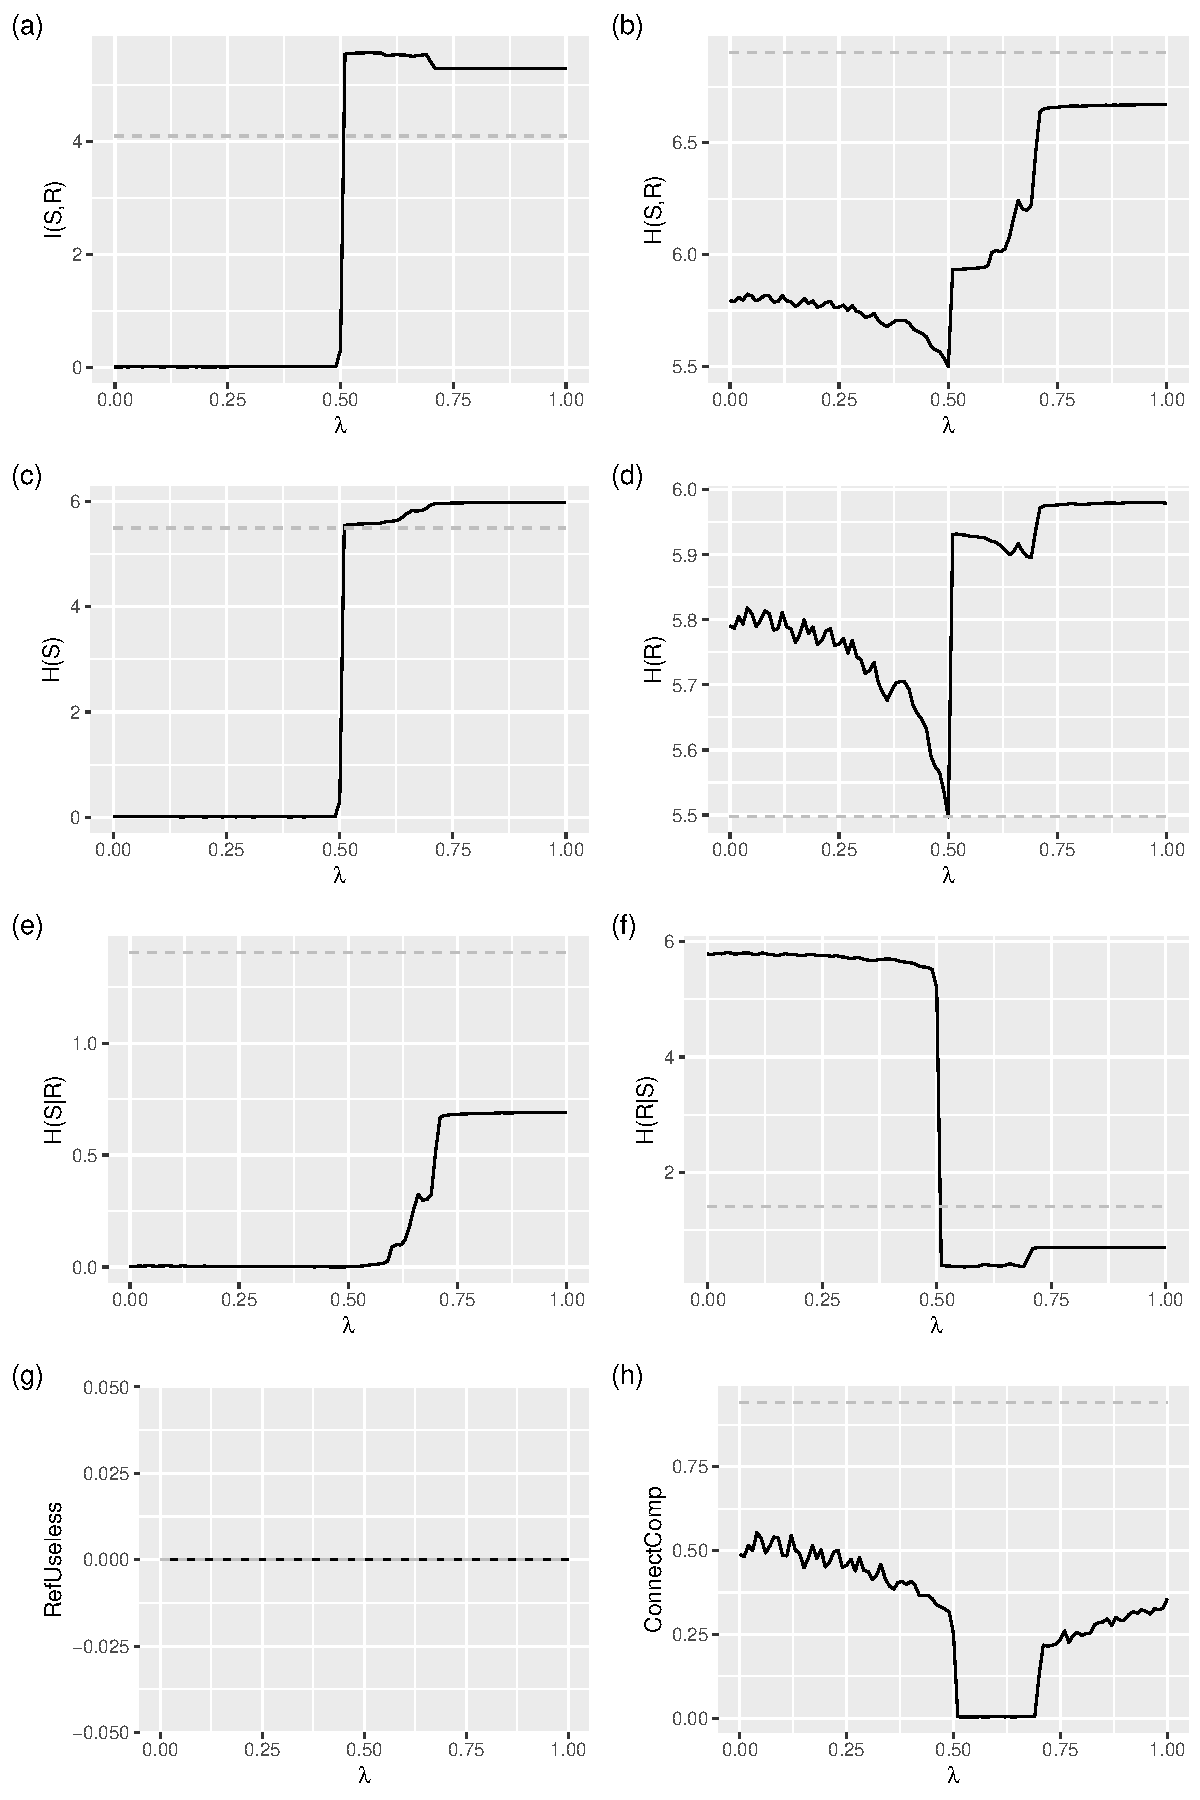
\includegraphics[height=0.7\textheight]{informationTheoretic_firstModel_phi1_nm400_dynamic_randomBipartite_allowUnlinked}
  \caption{Same information as in Figure \ref{fig:informationTheoretic_firstModel_phi0_nm400_dynamic_randomBipartite_allowUnlinked} but with $\phi=1$.}
  \label{fig:informationTheoretic_firstModel_phi1_nm400_dynamic_randomBipartite_allowUnlinked}
\end{figure}

\begin{figure}
  \centering
  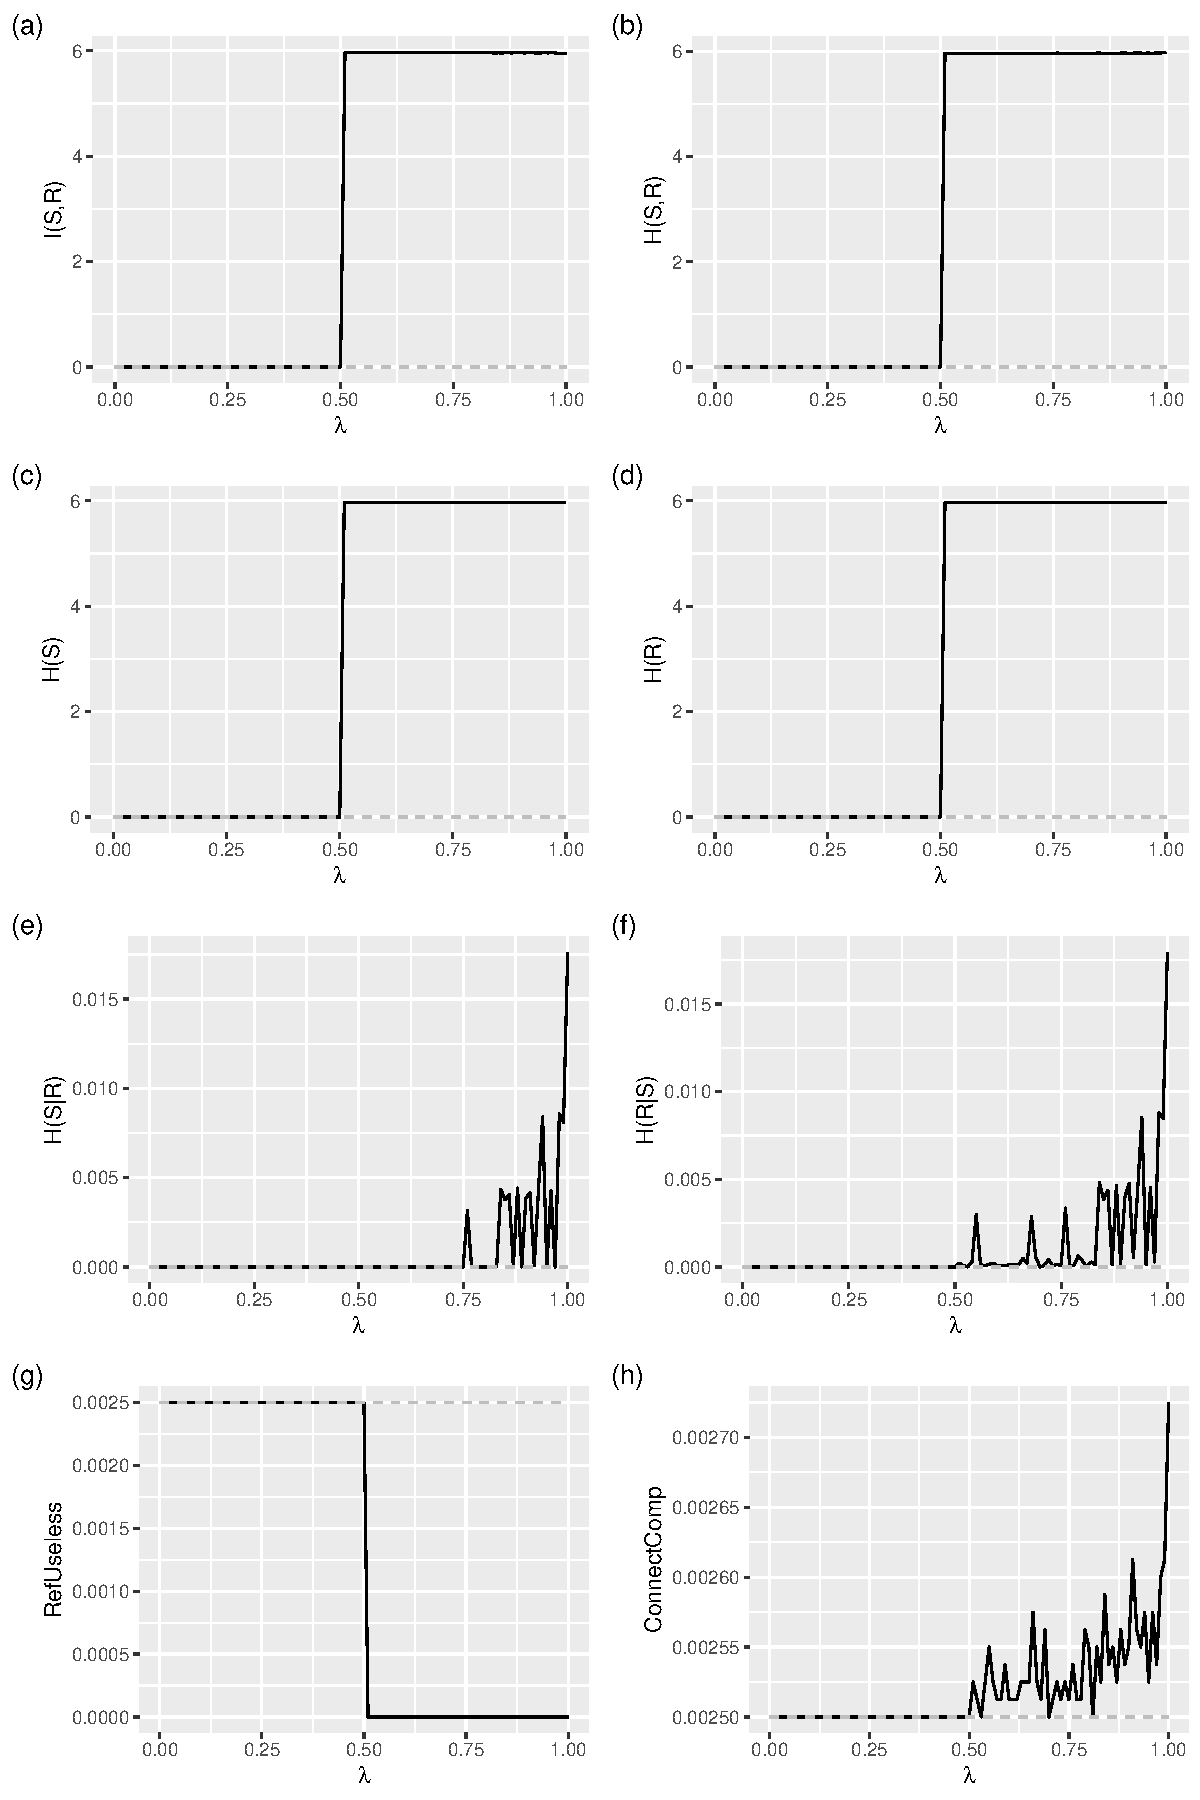
\includegraphics[height=0.7\textheight]{informationTheoretic_firstModel_phi1_nm400_dynamic_singleLink_allowUnlinked}
  \caption{Same information as in Figure \ref{fig:informationTheoretic_firstModel_phi0_nm400_dynamic_randomBipartite_allowUnlinked} but with $\phi=1$ and for a single link as the initial condition.}
  \label{fig:informationTheoretic_firstModel_phi1_nm400_dynamic_singleLink_allowUnlinked}
\end{figure}

\begin{figure}
  \centering
  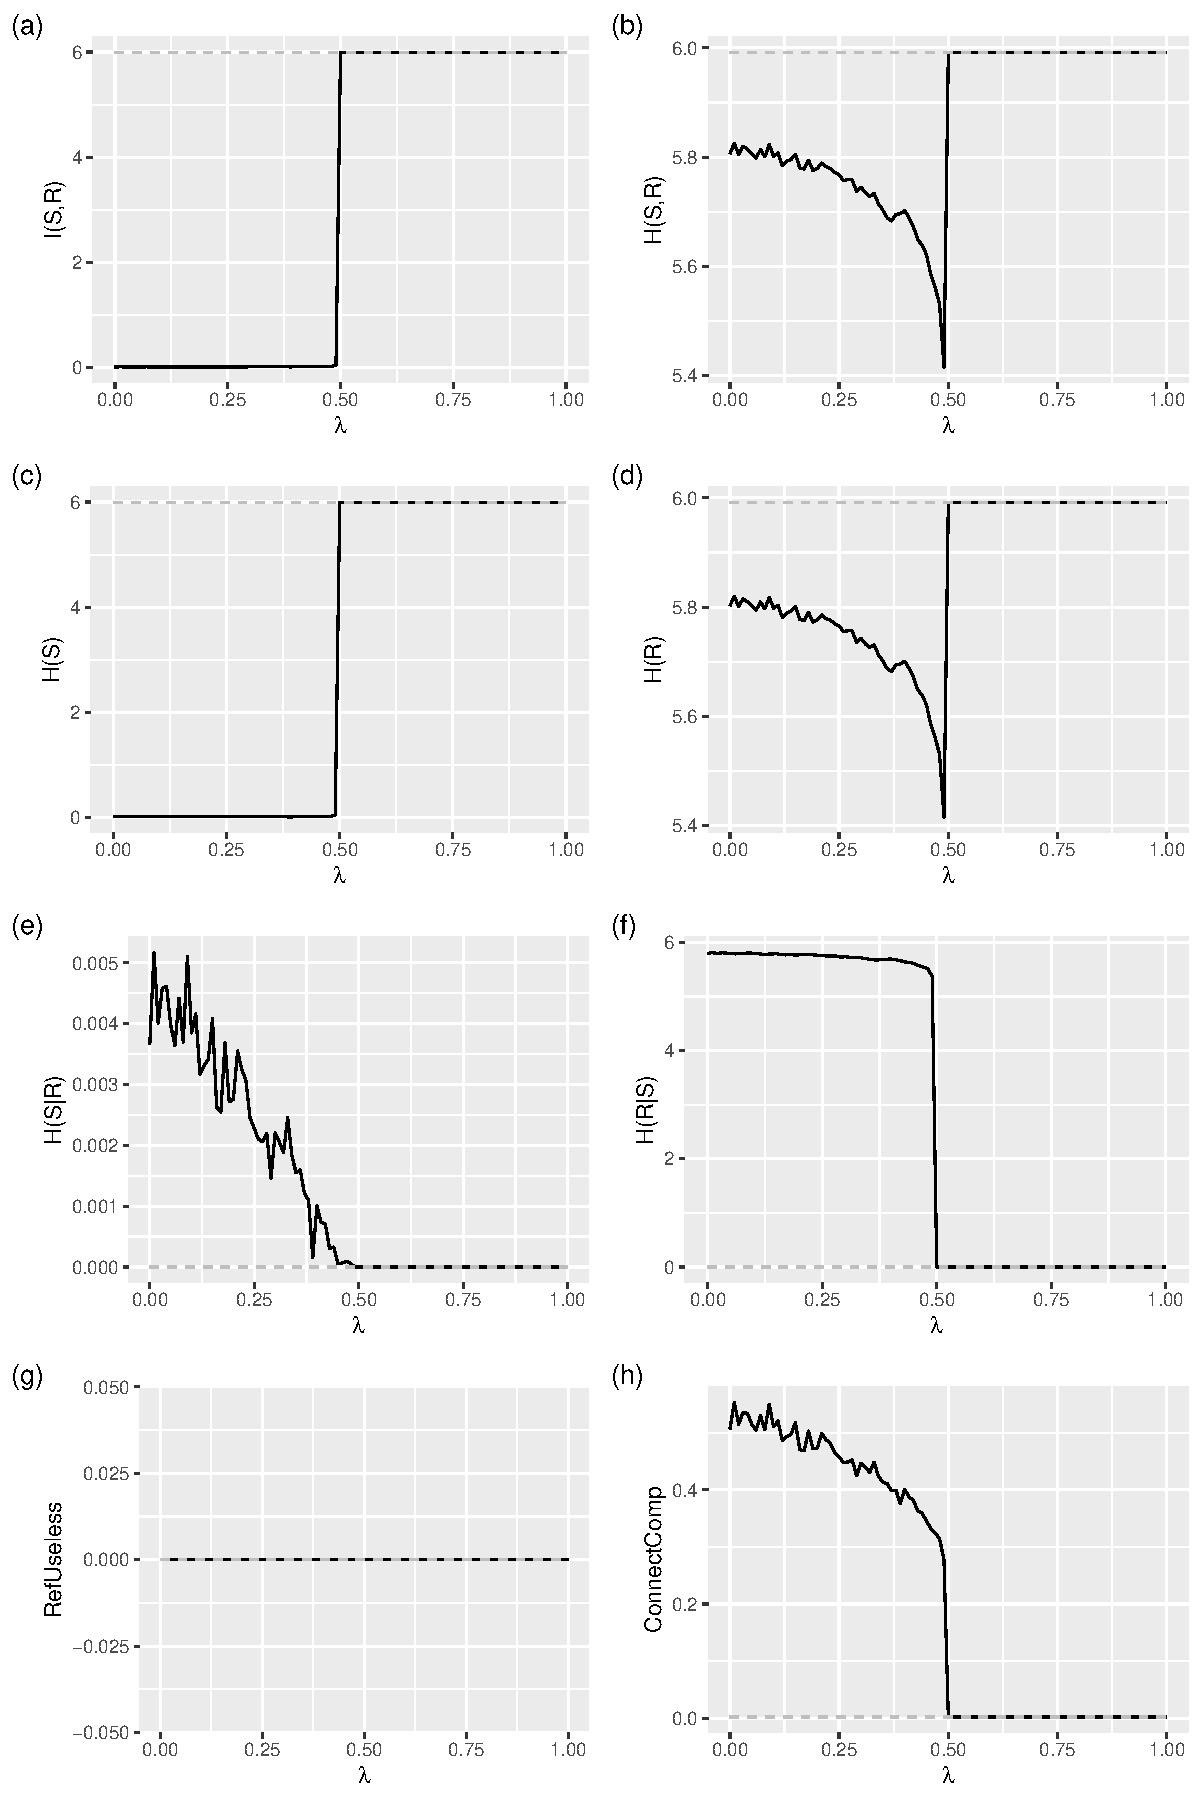
\includegraphics[height=0.7\textheight]{informationTheoretic_firstModel_phi1_nm400_dynamic_oneToOne_allowUnlinked}
  \caption{Same information as in Figure \ref{fig:informationTheoretic_firstModel_phi0_nm400_dynamic_randomBipartite_allowUnlinked} but with $\phi=1$ and for one to one connections between signals and meanings as the initial condition.}
  \label{fig:informationTheoretic_firstModel_phi1_nm400_dynamic_oneToOne_allowUnlinked}
\end{figure}

Figures \ref{fig:insideLambda_firstModel_phi1_nm400_dynamic_randomBipartite_allowUnlinked} and \ref{fig:insideLambda_firstModel_phi1_nm400_dynamic_oneToOne_allowUnlinked} (random and one-to-one initial conditions respectively) show statistical measures of select values of $\lambda$, with Figures \ref{fig:fitting_insideLambda_firstModel_phi1_nm400_dynamic_randomBipartite_allowUnlinked} and \ref{fig:fitting_insideLambda_firstModel_phi1_nm400_dynamic_oneToOne_allowUnlinked} (random and one-to-one respectively) showing the fitting of the curve to a power law for a single select value of $\lambda$.
However, in this case it's hard to say that the curves follow a power law.
Nevertheless, Tables \ref{tab:fitting_insideLambda_firstModel_phi1_nm400_dynamic_randomBipartite_allowUnlinked} and \ref{tab:fitting_insideLambda_firstModel_phi1_nm400_dynamic_oneToOne_allowUnlinked} (random and one-to-one respectively) show the values of the regression exponent and factor.
The single link initial condition is not plotted for select values of $\lambda$ as it fails to evolve beyond the single link state.

\begin{figure}
  \centering
  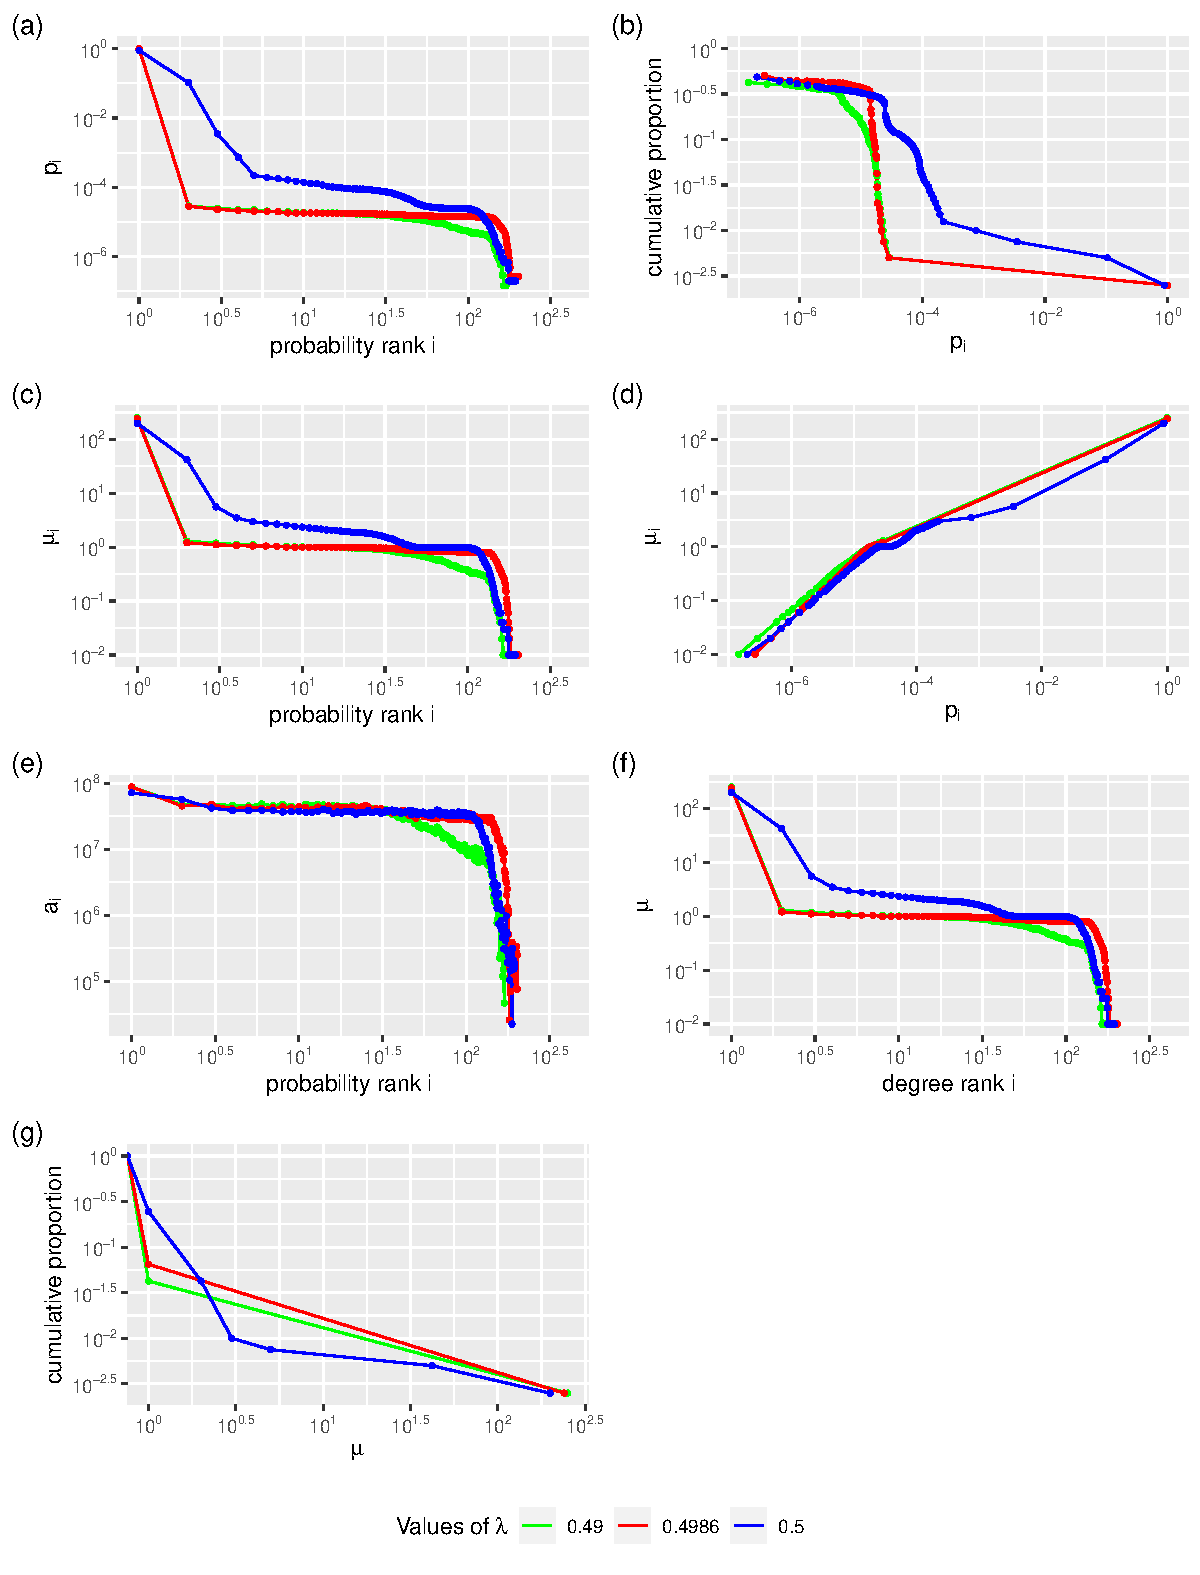
\includegraphics[height=0.7\textheight]{insideLambda_firstModel_phi1_nm400_dynamic_randomBipartite_allowUnlinked}
  \caption{Same information as in Figure \ref{fig:insideLambda_firstModel_phi0_nm400_dynamic_randomBipartite_allowUnlinked} but $\phi=1$. $\lambda^* = 0.4993$}
  \label{fig:insideLambda_firstModel_phi1_nm400_dynamic_randomBipartite_allowUnlinked}
\end{figure}

\begin{figure}
  \centering
  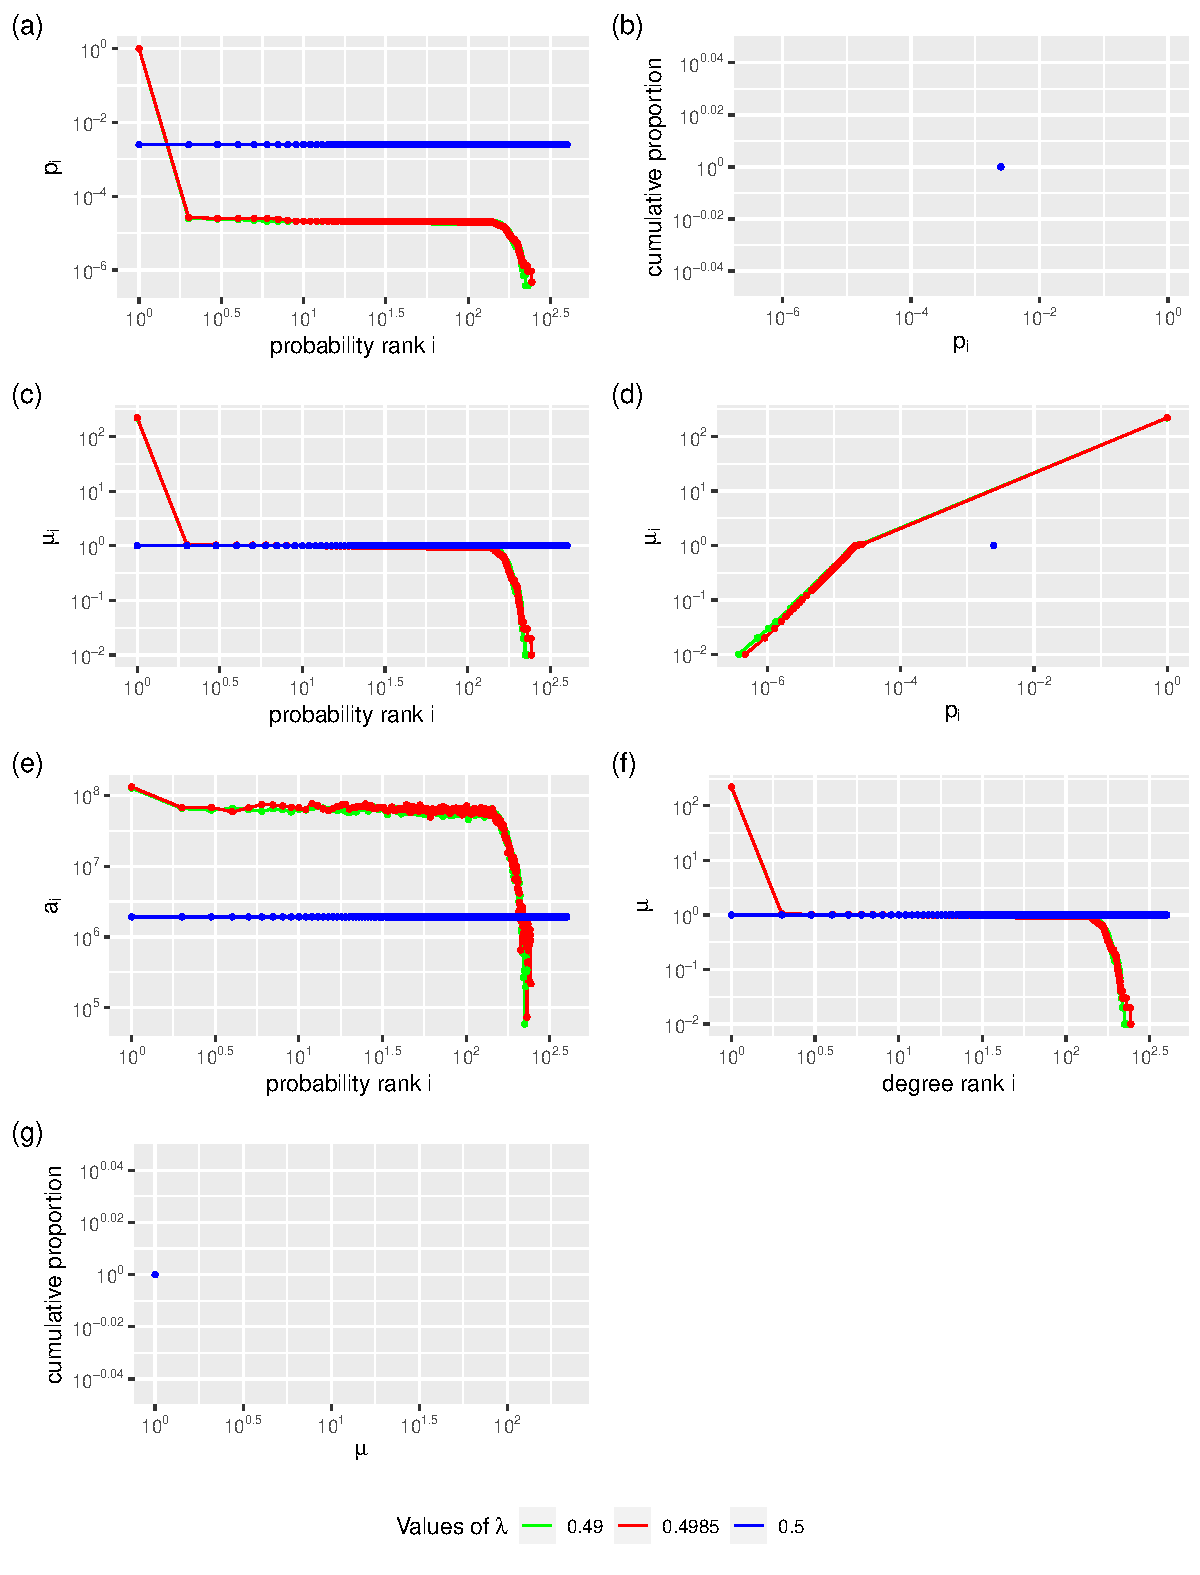
\includegraphics[height=0.7\textheight]{insideLambda_firstModel_phi1_nm400_dynamic_oneToOne_allowUnlinked}
  \caption{Same information as in Figure \ref{fig:insideLambda_firstModel_phi0_nm400_dynamic_randomBipartite_allowUnlinked} but $\phi=1$ and the initial condition is one to one connections between words and meanings. $\lambda^* = 0.4986$}
  \label{fig:insideLambda_firstModel_phi1_nm400_dynamic_oneToOne_allowUnlinked}
\end{figure}

\begin{figure}
  \centering
  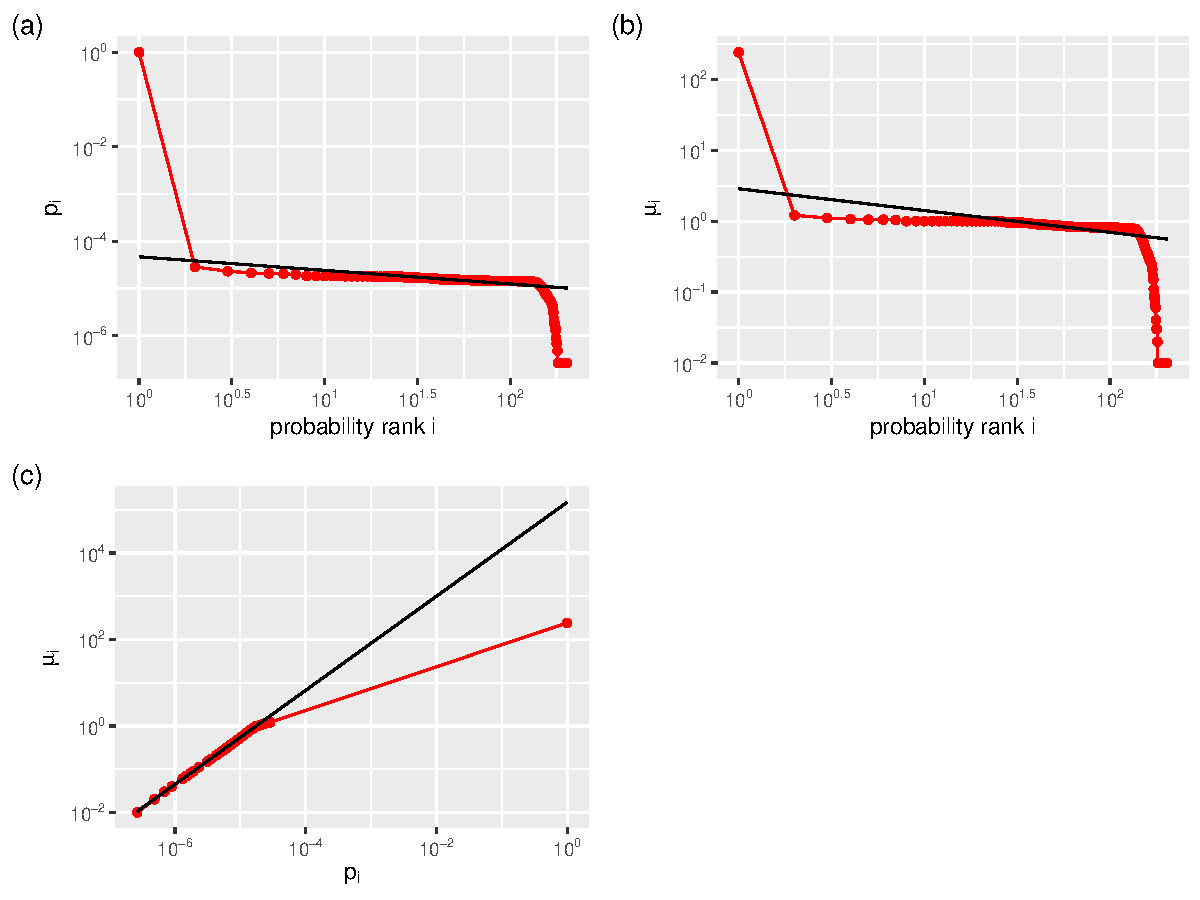
\includegraphics[width=\textwidth]{fitting_insideLambda_firstModel_phi1_nm400_dynamic_randomBipartite_allowUnlinked}
  \caption{Same information as in Figure \ref{fig:fitting_insideLambda_firstModel_phi0_nm400_dynamic_randomBipartite_allowUnlinked} but $\phi=1$. $\lambda^*=0.4986$.
Table \ref{tab:fitting_insideLambda_firstModel_phi1_nm400_dynamic_randomBipartite_allowUnlinked} shows the values of the exponent and the factor of the fitted power law.}
  \label{fig:fitting_insideLambda_firstModel_phi1_nm400_dynamic_randomBipartite_allowUnlinked}
\end{figure}

\begin{figure}
  \centering
  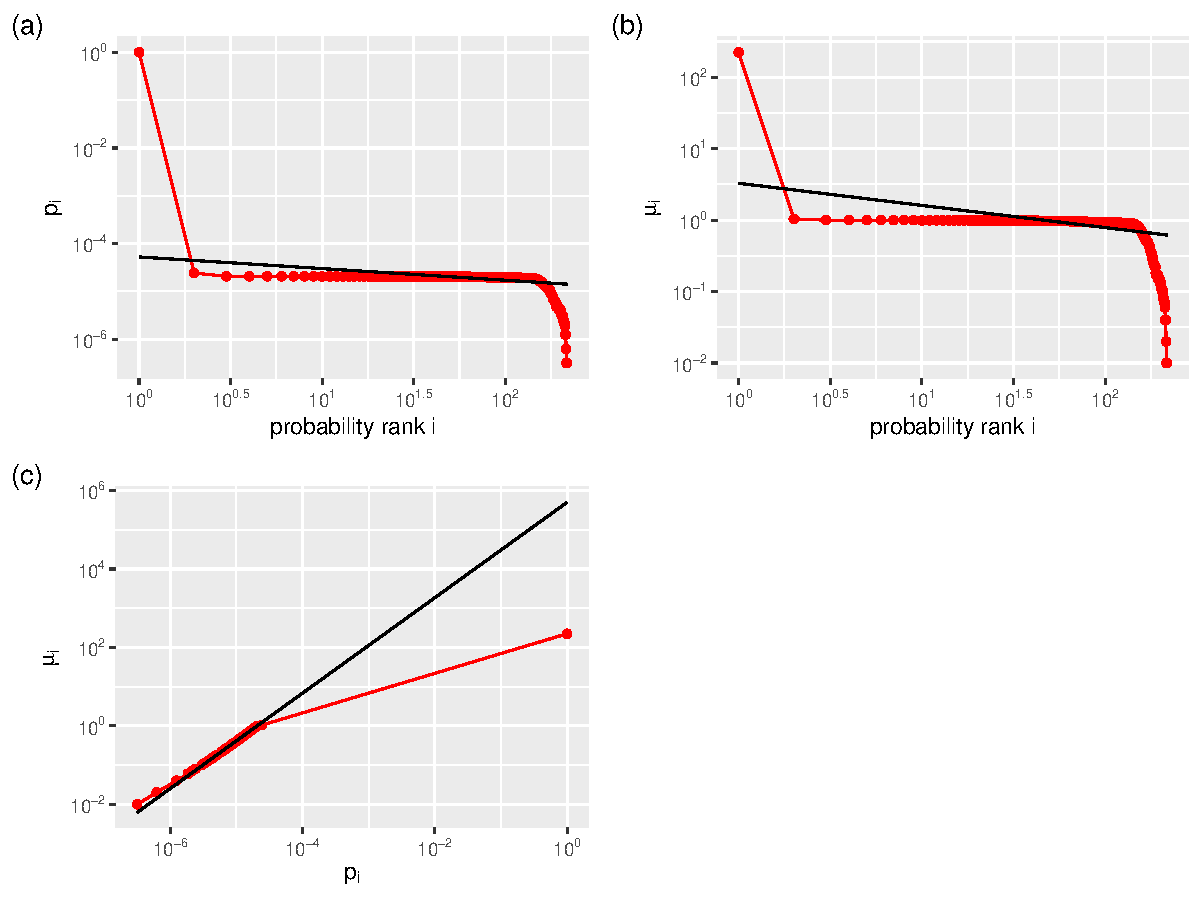
\includegraphics[width=\textwidth]{fitting_insideLambda_firstModel_phi1_nm400_dynamic_oneToOne_allowUnlinked}
  \caption{Same information as in Figure \ref{fig:fitting_insideLambda_firstModel_phi0_nm400_dynamic_randomBipartite_allowUnlinked} but $\phi=1$ and the initial condition is one to one connections between words and meanings. $\lambda^*=0.4993$.
Table \ref{tab:fitting_insideLambda_firstModel_phi1_nm400_dynamic_oneToOne_allowUnlinked} shows the values of the exponent and the factor of the fitted power law.}
  \label{fig:fitting_insideLambda_firstModel_phi1_nm400_dynamic_oneToOne_allowUnlinked}
\end{figure}

% latex table generated in R 4.0.4 by xtable 1.8-4 package
% Wed Mar 17 14:32:51 2021
\begin{table}[ht]
\centering
\begin{tabular}{lrr}
  \hline
plot & alpha & k \\ 
  \hline
a & -0.2871434 & 0.0000468 \\ 
  b & -2.5493723 & 0.0000000 \\ 
  c & -0.3072861 & 2.8668125 \\ 
  d & 1.0876280 & 149669.1453764 \\ 
  f & -0.3072861 & 2.8668125 \\ 
  g & -0.5944739 & 0.0650000 \\ 
   \hline
\end{tabular}
\caption{caption} 
\label{tables/fitting_insideLambda_firstModel_phi1_nm400_dynamic_randomBipartite_allowUnlinked}
\end{table}


% latex table generated in R 4.0.4 by xtable 1.8-4 package
% Wed Mar 17 14:56:06 2021
\begin{table}[ht]
\centering
\begin{tabular}{lrr}
  \hline
plot & $\alpha$ & $k$ \\ 
  \hline
a & 0.2433438 & 0.0000524 \\ 
  b & 2.2902299 & 0.0000000 \\ 
  c & 0.3100715 & 3.2784604 \\ 
  d & -1.2166546 & 501643.7856344 \\ 
  f & 0.3100715 & 3.2784604 \\ 
  g & 0.4063538 & 0.0225000 \\ 
   \hline
\end{tabular}
\caption{Table showing the exponent and factor of the power laws fitted in Figure \ref{fig:fitting_insideLambda_firstModel_phi1_nm400_dynamic_oneToOne_allowUnlinked}} 
\label{tab:fitting_insideLambda_firstModel_phi1_nm400_dynamic_oneToOne_allowUnlinked}
\end{table}


For the \secondmodel{} with $\phi=0$ Figures  \ref{fig:informationTheoretic_uniform_phi0_nm400_dynamic_randomBipartite_allowUnlinked},  \ref{fig:informationTheoretic_uniform_phi0_nm400_dynamic_singleLink_allowUnlinked} and  \ref{fig:informationTheoretic_uniform_phi0_nm400_dynamic_oneToOne_allowUnlinked} show the information theoretic measures of the optimal graph for values of $\lambda$ ranging from 0 to 1.
They correspond to the random graph, single link and one-to-one initial graphs respectively.
Appendix \ref{sec:app_figures_second-model} shows the same figures but with disconnected meanings disallowed.

\begin{figure}
  \centering
  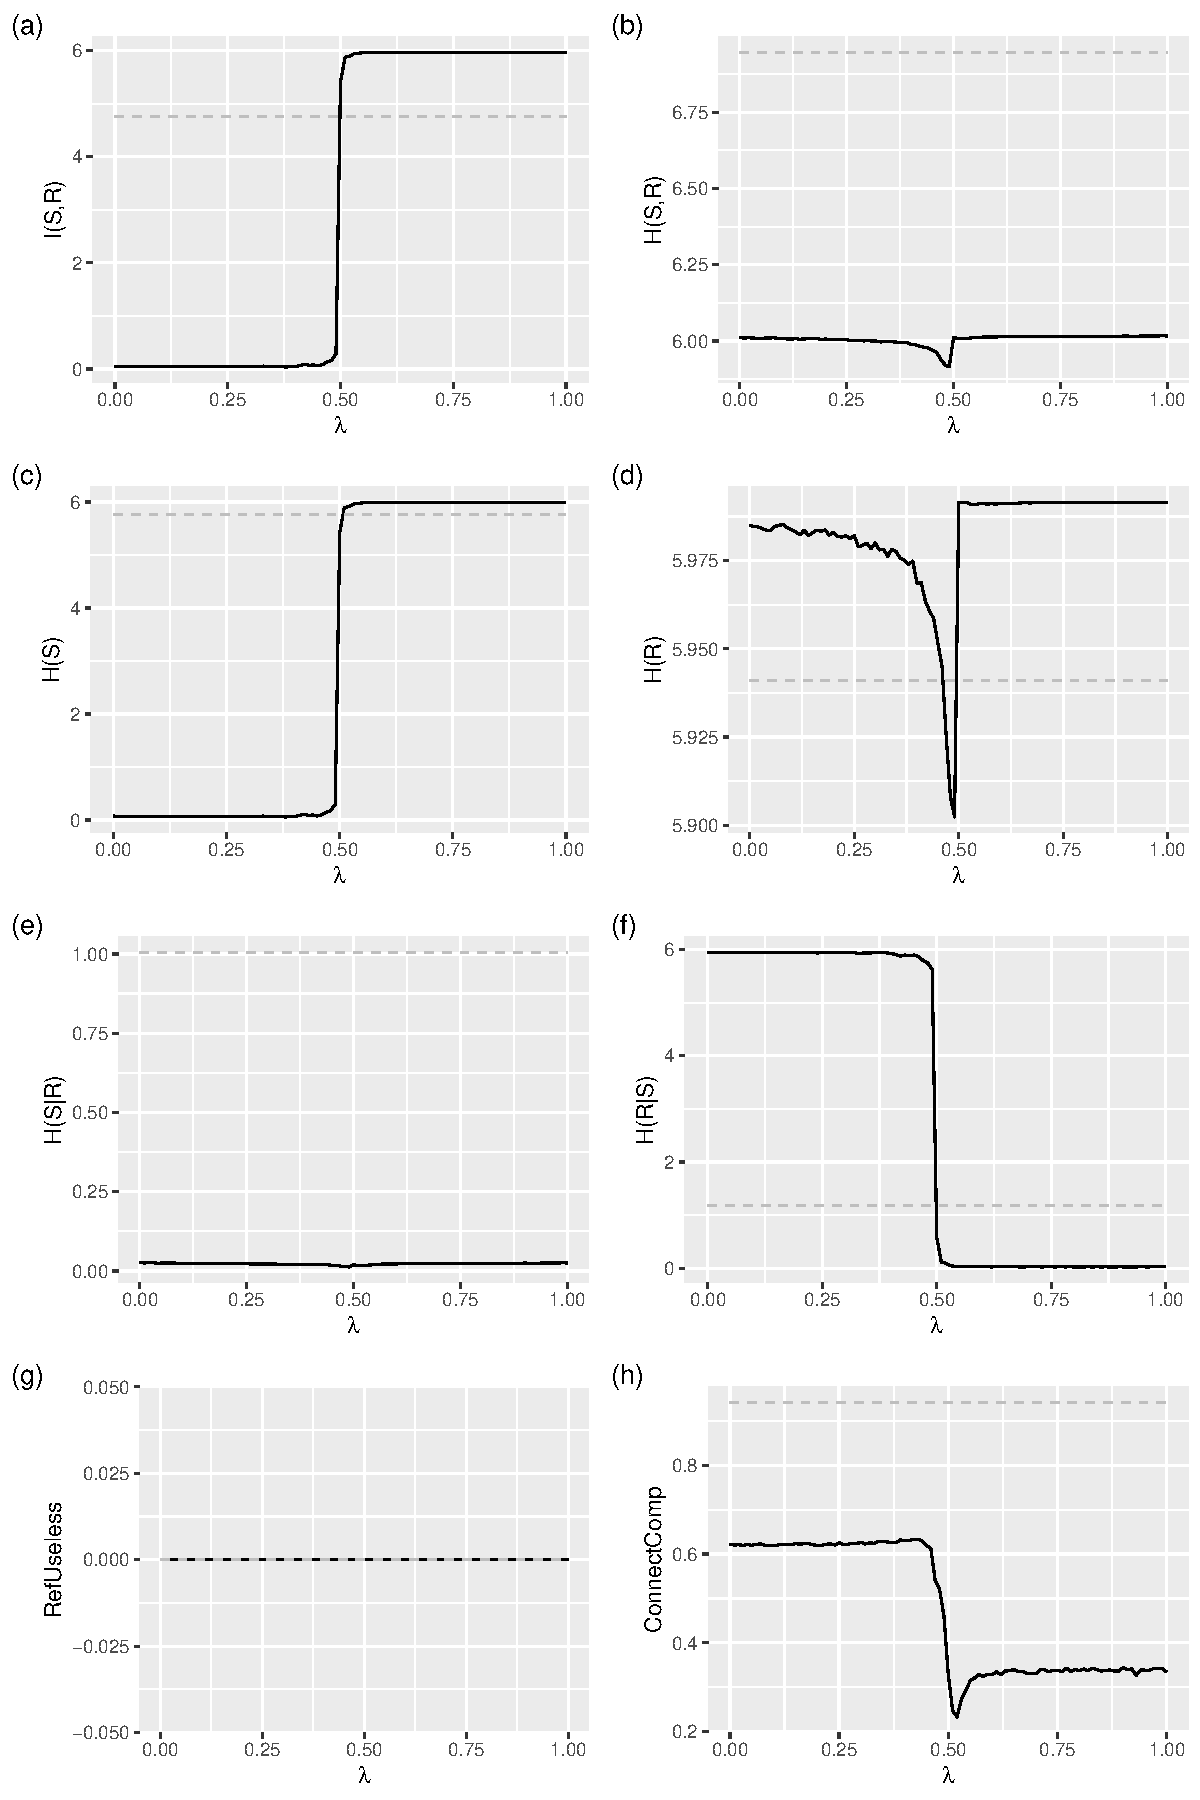
\includegraphics[height=0.7\textheight]{informationTheoretic_uniform_phi0_nm400_dynamic_randomBipartite_allowUnlinked}
  \caption{Same information as in Figure \ref{fig:informationTheoretic_firstModel_phi0_nm400_dynamic_randomBipartite_allowUnlinked} but the graph uses the equations of the \secondmodel{} with $\pi$ following a uniform distribution.}
  \label{fig:informationTheoretic_uniform_phi0_nm400_dynamic_randomBipartite_allowUnlinked}
\end{figure}

\begin{figure}
  \centering
  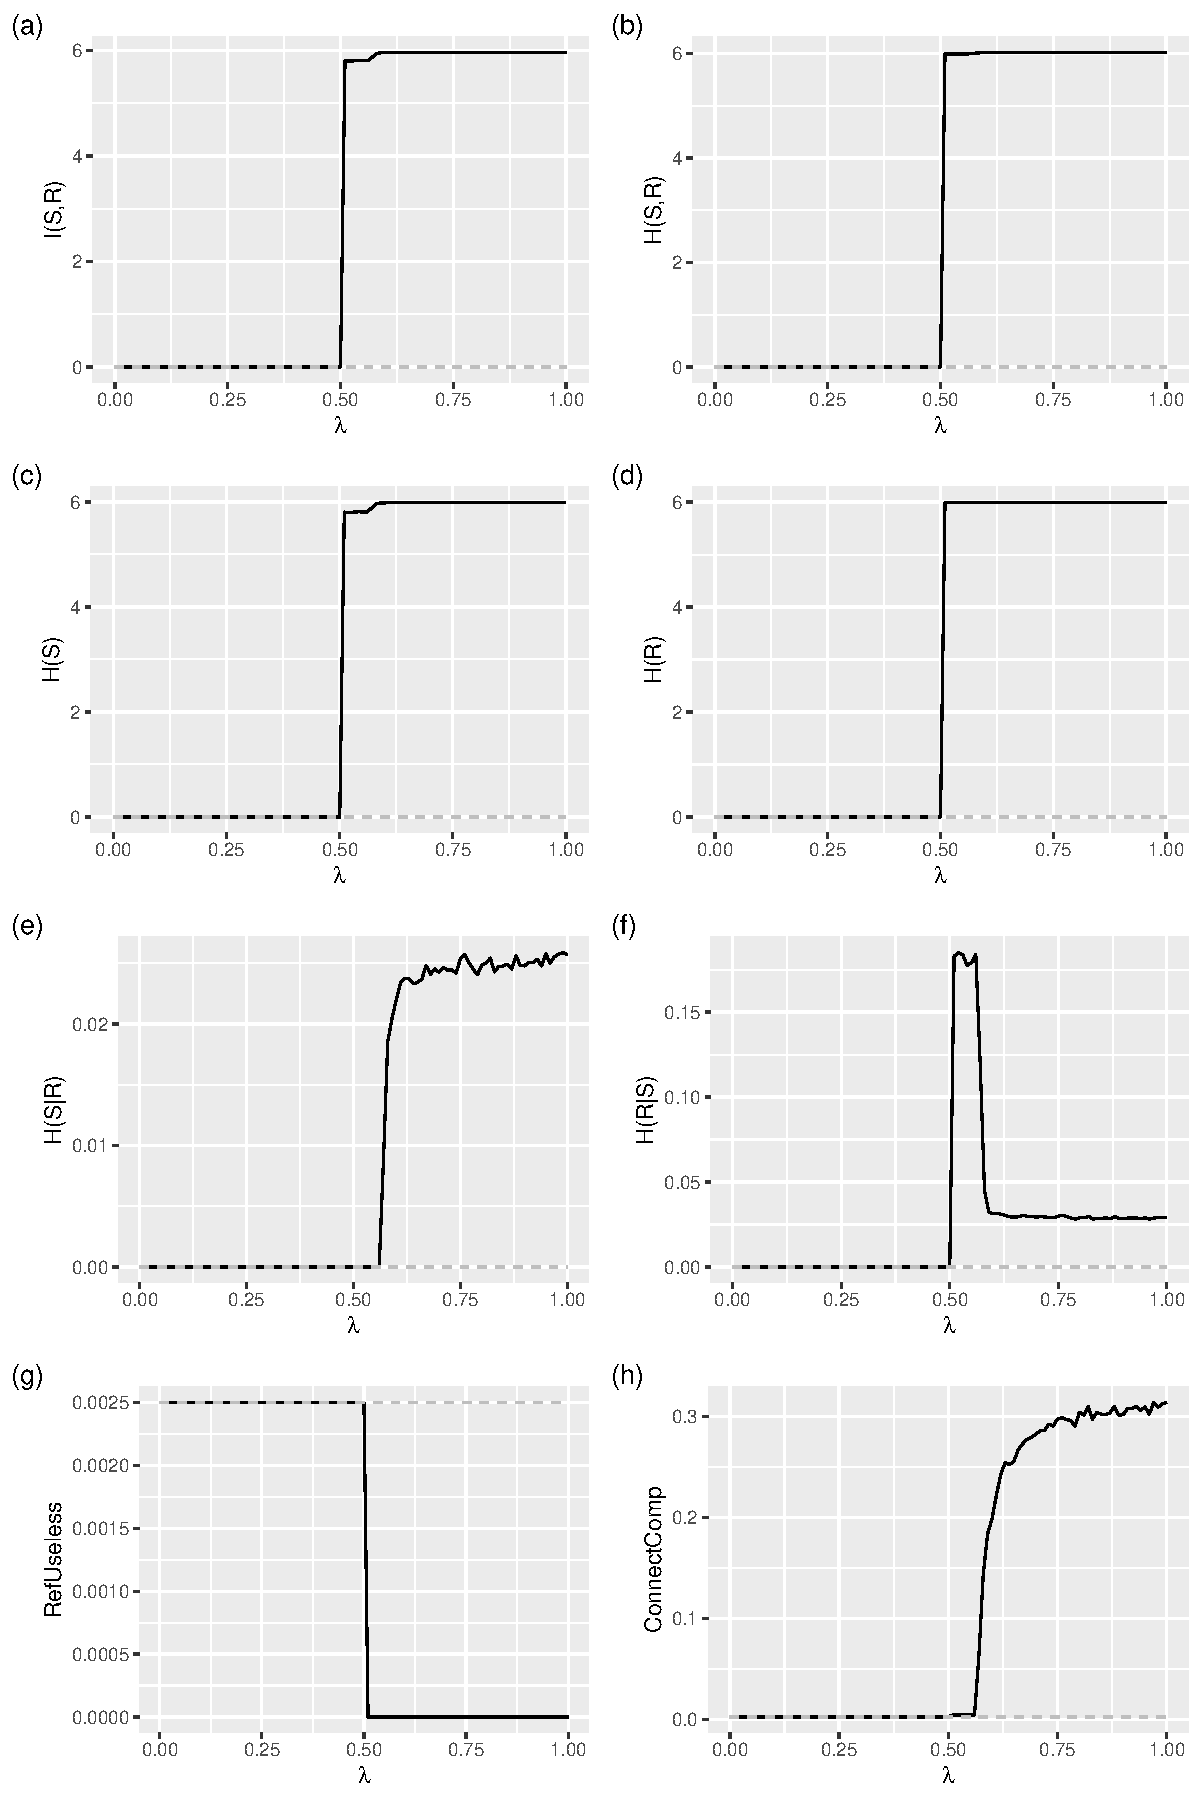
\includegraphics[height=0.7\textheight]{informationTheoretic_uniform_phi0_nm400_dynamic_singleLink_allowUnlinked}
  \caption{Same information as in Figure \ref{fig:informationTheoretic_firstModel_phi0_nm400_dynamic_randomBipartite_allowUnlinked} but the graph uses the equations of the \secondmodel{} with $\pi$ following a uniform distribution and the initial condition is a single link}
  \label{fig:informationTheoretic_uniform_phi0_nm400_dynamic_singleLink_allowUnlinked}
\end{figure}

\begin{figure}
  \centering
  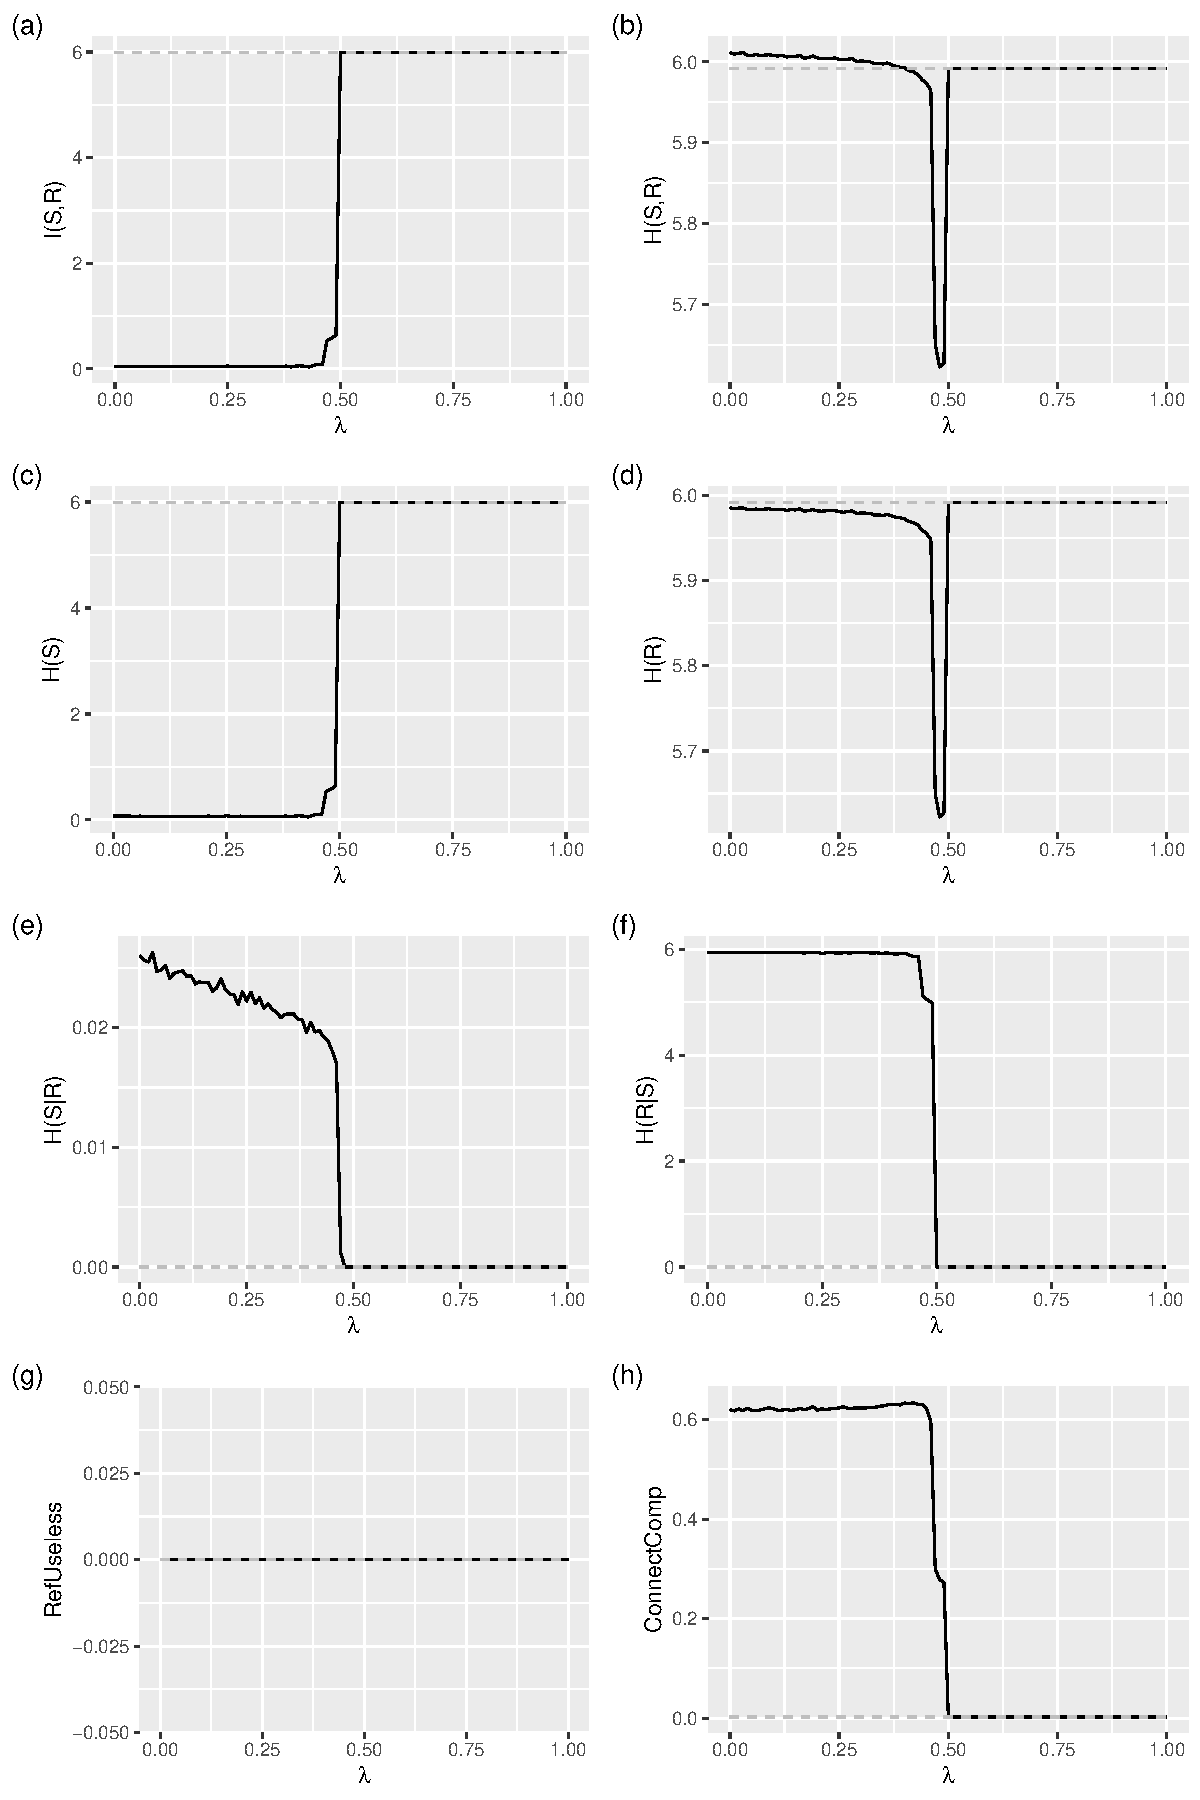
\includegraphics[height=0.7\textheight]{informationTheoretic_uniform_phi0_nm400_dynamic_oneToOne_allowUnlinked}
  \caption{Same information as in Figure \ref{fig:informationTheoretic_firstModel_phi0_nm400_dynamic_randomBipartite_allowUnlinked} but the graph uses the equations of the \secondmodel{} with $\pi$ following a uniform distribution and the initial condition is one to one connections between signals and meanings.}
  \label{fig:informationTheoretic_uniform_phi0_nm400_dynamic_oneToOne_allowUnlinked}
\end{figure}


Figures \ref{fig:insideLambda_uniform_phi0_nm400_dynamic_randomBipartite_allowUnlinked} and \ref{fig:insideLambda_uniform_phi0_nm400_dynamic_oneToOne_allowUnlinked} (random and one-to-one respectively) show statistical measures of select values of $\lambda$, with Figures \ref{fig:fitting_insideLambda_uniform_phi0_nm400_dynamic_randomBipartite_allowUnlinked} and \ref{fig:fitting_insideLambda_uniform_phi0_nm400_dynamic_oneToOne_allowUnlinked} (random and one-to-one respectively) showing the fitting of the curve to a power law for a single select value of $\lambda$.
A power law is appreciated in some of the plots but not all of them.
Tables \ref{tab:fitting_insideLambda_uniform_phi0_nm400_dynamic_randomBipartite_allowUnlinked} and \ref{tab:fitting_insideLambda_uniform_phi0_nm400_dynamic_oneToOne_allowUnlinked} (random and one-to-one respectively) show the values of the regression exponent and factor.
As with others, the single link initial condition is not plotted for select values of $\lambda$ as it fails to evolve beyond the single link state.
Appendix \ref{sec:app_figures_second-model} shows the same figures but with disconnected meanings disallowed.

\begin{figure}
  \centering
  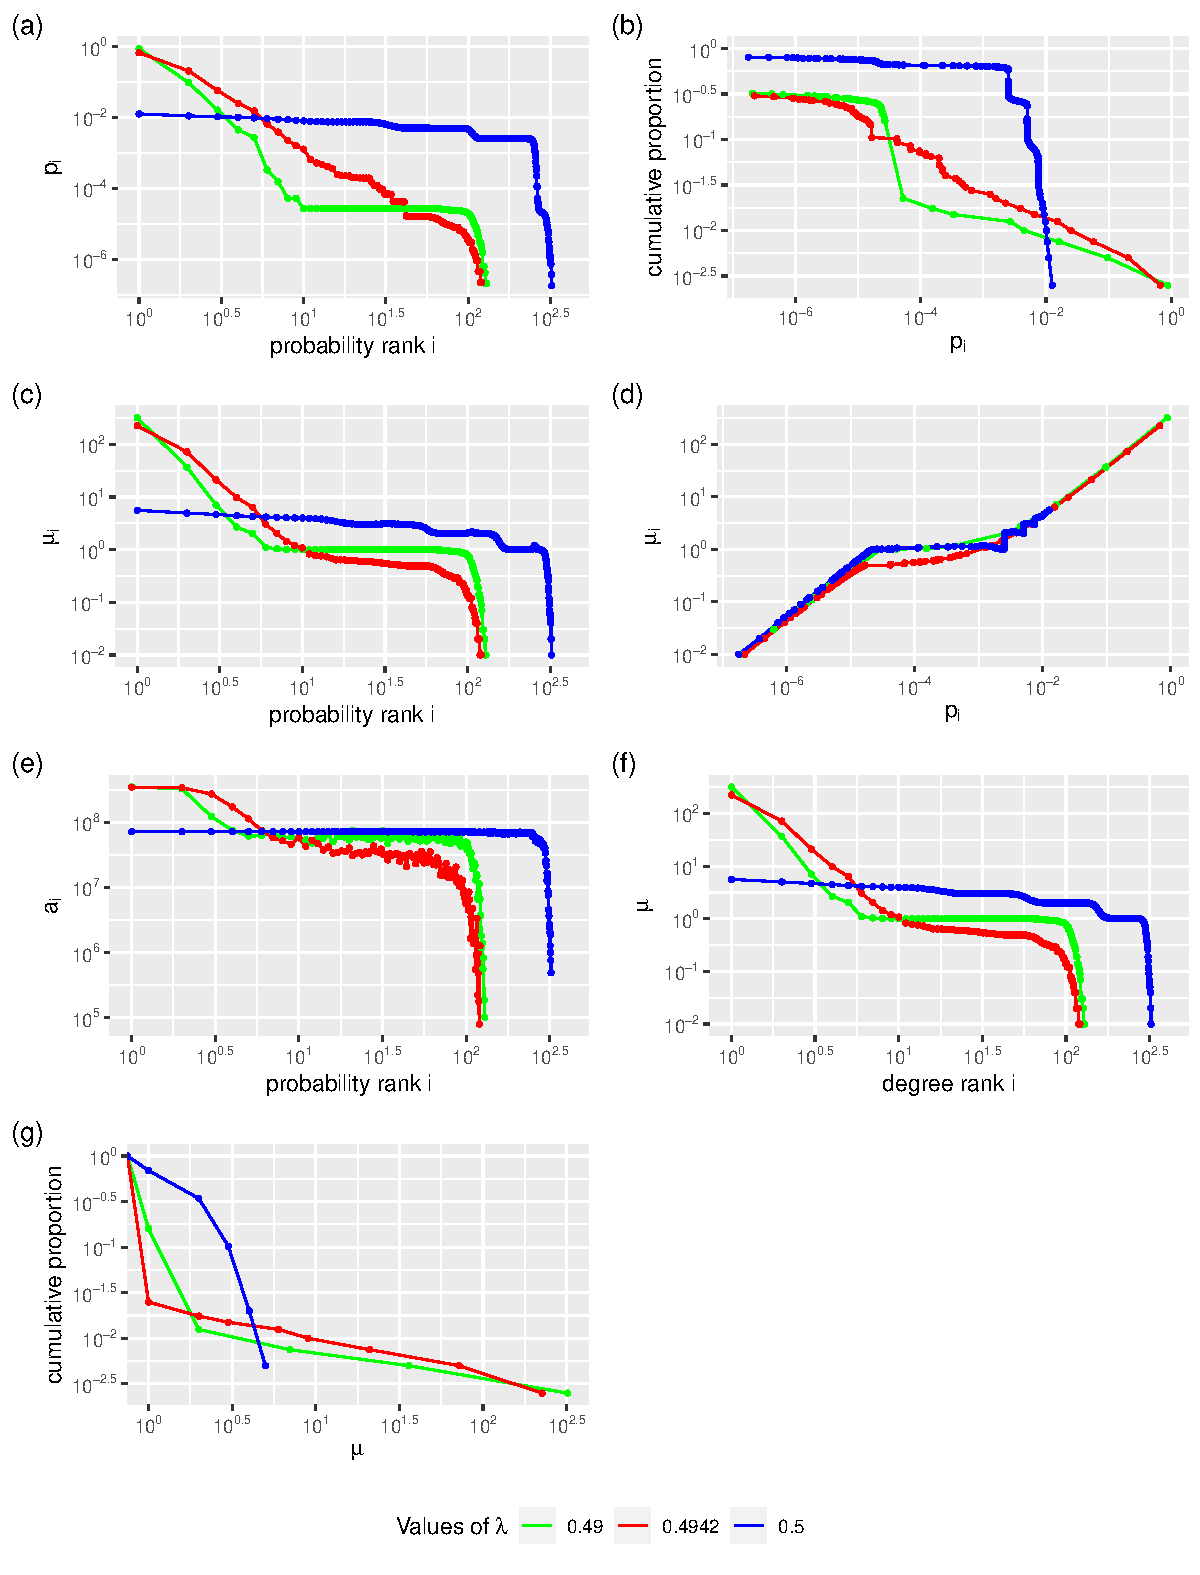
\includegraphics[height=0.7\textheight]{insideLambda_uniform_phi0_nm400_dynamic_randomBipartite_allowUnlinked}
  \caption{Same information as in Figure \ref{fig:insideLambda_firstModel_phi0_nm400_dynamic_randomBipartite_allowUnlinked} but the graph follows the equations of the \secondmodel{} with $\pi$ following a uniform distribution. $\lambda^* = 0.4942$}
  \label{fig:insideLambda_uniform_phi0_nm400_dynamic_randomBipartite_allowUnlinked}
\end{figure}

\begin{figure}
  \centering
  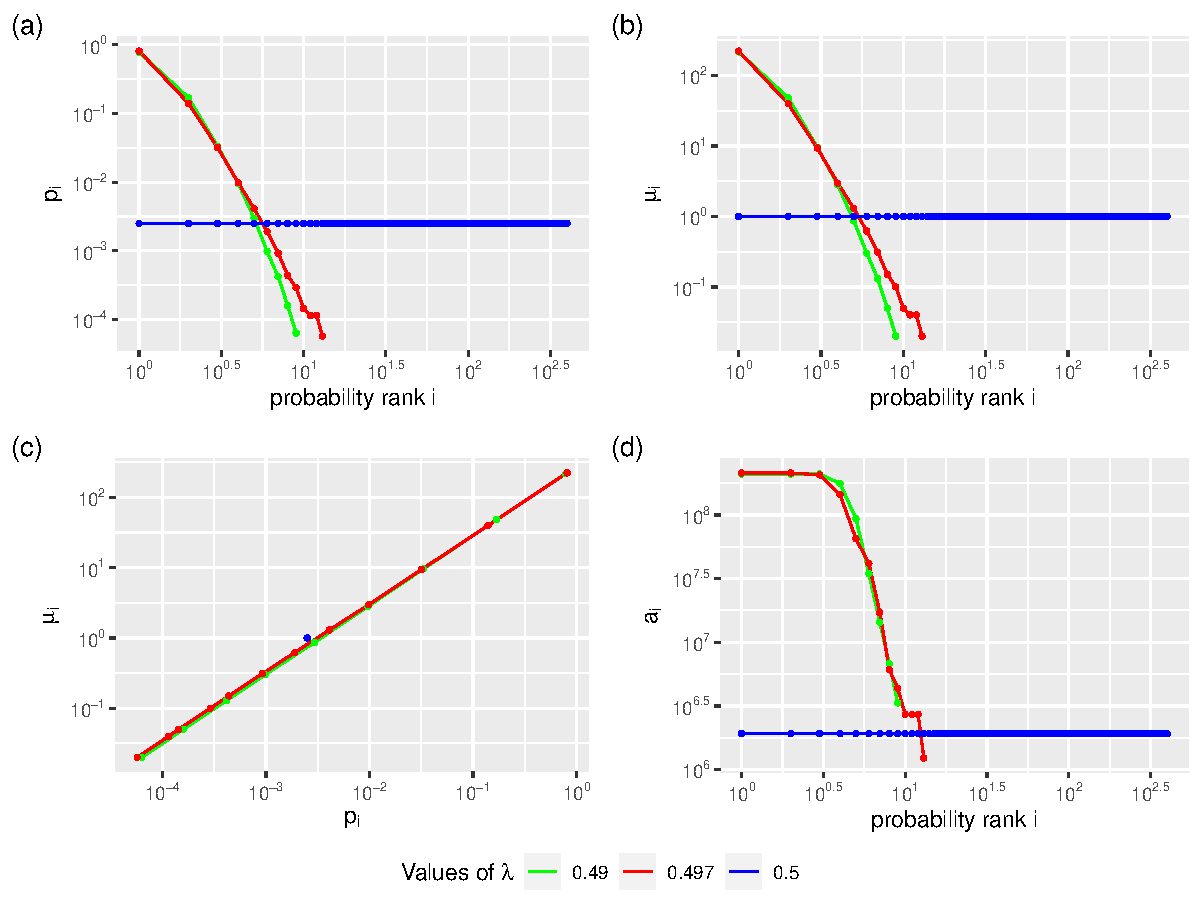
\includegraphics[height=0.7\textheight]{insideLambda_uniform_phi0_nm400_dynamic_oneToOne_allowUnlinked.pdf}
  \caption{Same information as in Figure \ref{fig:insideLambda_firstModel_phi0_nm400_dynamic_randomBipartite_allowUnlinked} but the graph follows the equations of the \secondmodel{} with $\pi$ following a uniform distribution and the initial condition is one to one connections between words and meanings. $\lambda^* = 0.4970$}
  \label{fig:insideLambda_uniform_phi0_nm400_dynamic_oneToOne_allowUnlinked}
\end{figure}

\begin{figure}
  \centering
  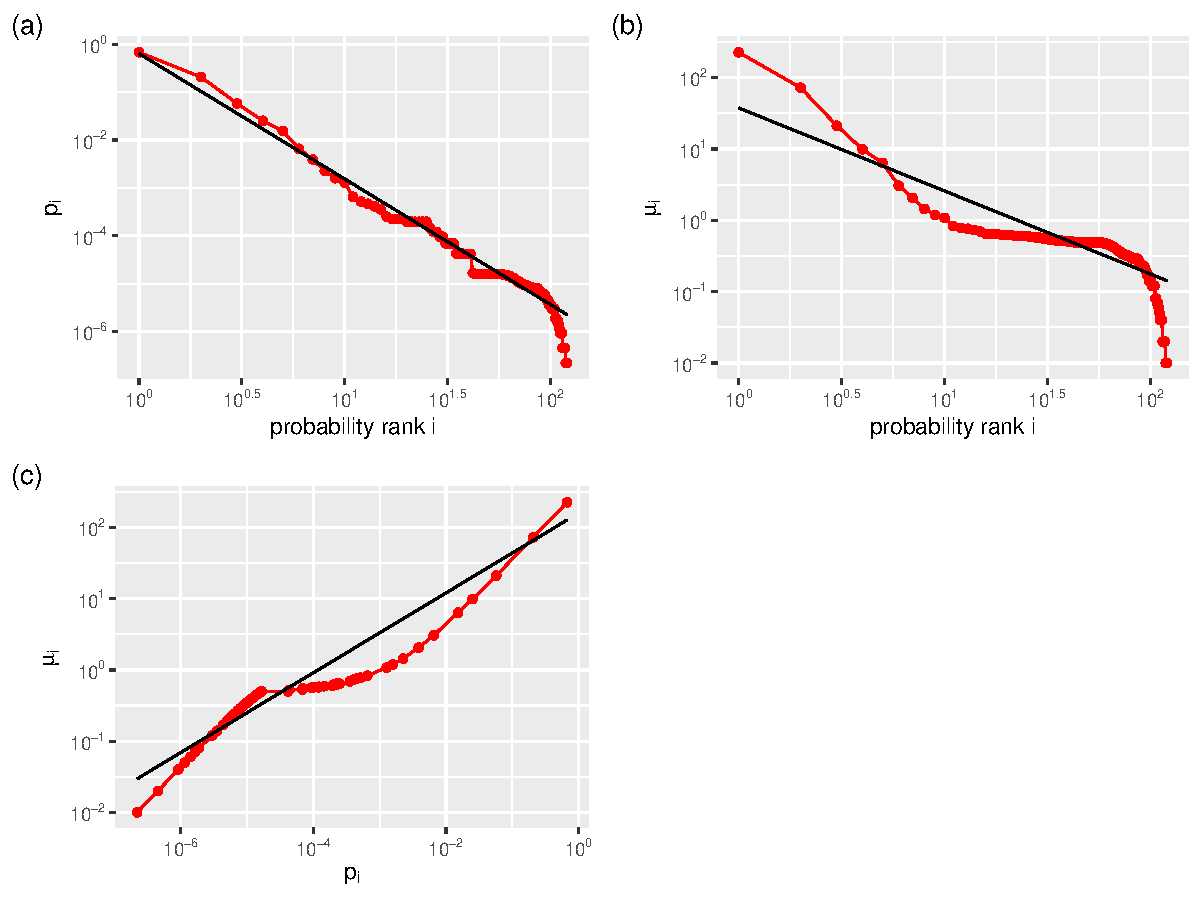
\includegraphics[width=\textwidth]{fitting_insideLambda_uniform_phi0_nm400_dynamic_randomBipartite_allowUnlinked}
  \caption{Same information as in Figure \ref{fig:fitting_insideLambda_firstModel_phi0_nm400_dynamic_randomBipartite_allowUnlinked} but the model follows the equations of the \secondmodel{} with $\pi$ following a uniform distribution. $\lambda^*=0.4942$.
Table \ref{tab:fitting_insideLambda_uniform_phi0_nm400_dynamic_randomBipartite_allowUnlinked} shows the values of the exponent and the factor of the fitted power law.}
  \label{fig:fitting_insideLambda_uniform_phi0_nm400_dynamic_randomBipartite_allowUnlinked}
\end{figure}

\begin{figure}
  \centering
  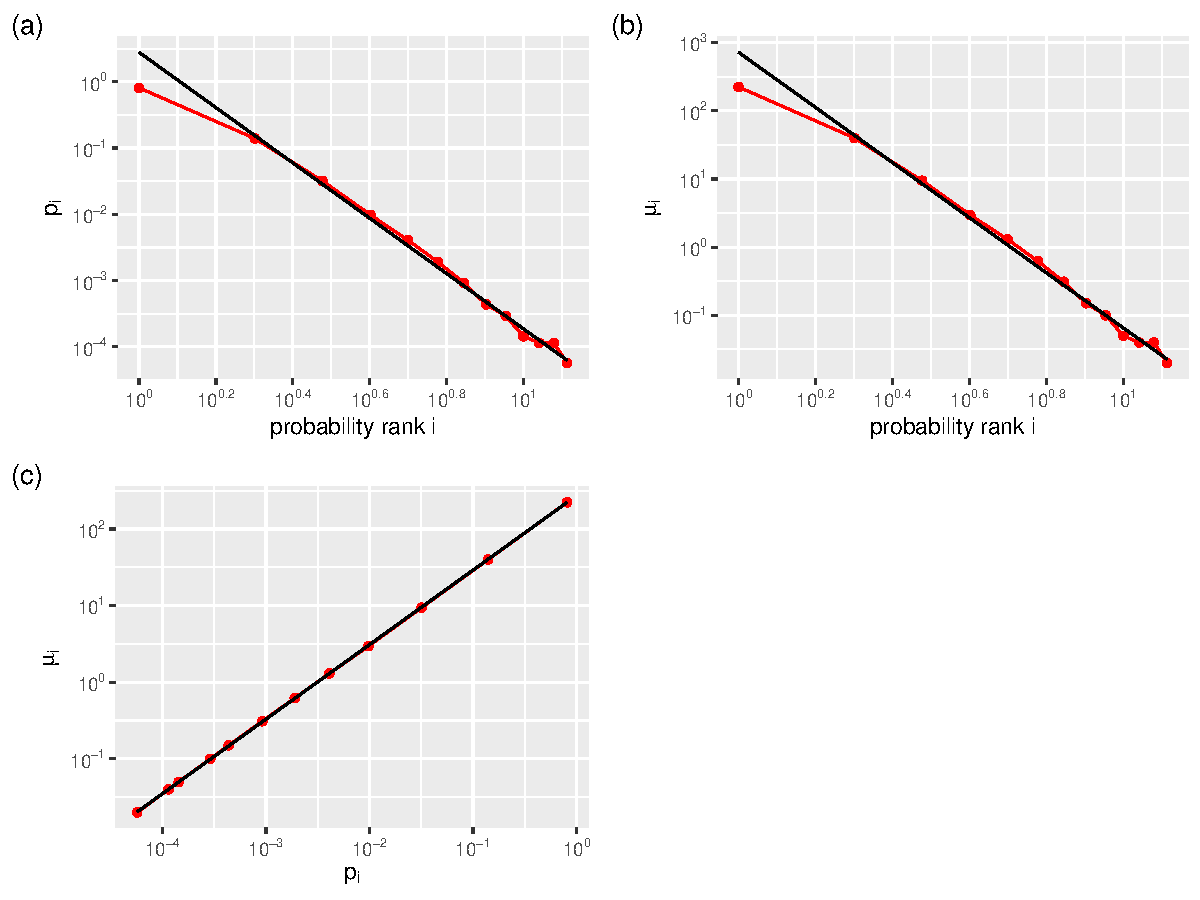
\includegraphics[width=\textwidth]{fitting_insideLambda_uniform_phi0_nm400_dynamic_oneToOne_allowUnlinked}
  \caption{Same information as in Figure \ref{fig:fitting_insideLambda_firstModel_phi0_nm400_dynamic_randomBipartite_allowUnlinked} but the model follows the equations of the \secondmodel{} with $\pi$ following a uniform distribution and the initial condition is one to one connections between words and meanings. $\lambda^*=0.4970$.
Table \ref{tab:fitting_insideLambda_uniform_phi0_nm400_dynamic_oneToOne_allowUnlinked} shows the values of the exponent and the factor of the fitted power law.}
  \label{fig:fitting_insideLambda_uniform_phi0_nm400_dynamic_oneToOne_allowUnlinked}
\end{figure}

% latex table generated in R 4.1.1 by xtable 1.8-4 package
% Sat Oct  2 23:05:07 2021
\begin{table}[ht]
\centering
\begin{tabular}{lrr}
  \hline
plot & $\alpha$ & $k$ \\ 
  \hline
a & 2.6176507 & 0.6341345 \\ 
  b & 0.3812498 & 0.0021506 \\ 
  c & 1.1623482 & 37.4616016 \\ 
  d & -0.5600378 & 158.5629462 \\ 
  f & 1.1623482 & 37.4616016 \\ 
  g & 0.3954554 & 0.0250000 \\ 
   \hline
\end{tabular}
\caption{Table showing the exponent and factor of the power laws fitted in Figure \ref{fig:fitting_insideLambda_uniform_phi0_nm400_dynamic_randomBipartite_allowUnlinked}} 
\label{tab:fitting_insideLambda_uniform_phi0_nm400_dynamic_randomBipartite_allowUnlinked}
\end{table}


% latex table generated in R 4.1.1 by xtable 1.8-4 package
% Sun Oct  3 00:21:42 2021
\begin{table}[ht]
\centering
\begin{tabular}{lrr}
  \hline
plot & $\alpha$ & $k$ \\ 
  \hline
a & 4.1719196 & 2.7845870 \\ 
  b & 0.2458167 & 0.0031418 \\ 
  c & 4.0408414 & 717.6995365 \\ 
  d & -0.9728453 & 272.7810669 \\ 
  f & 4.0408414 & 717.6995365 \\ 
  g & 0.2854165 & 0.0125000 \\ 
   \hline
\end{tabular}
\caption{Table showing the exponent and factor of the power laws fitted in Figure \ref{fig:fitting_insideLambda_uniform_phi0_nm400_dynamic_oneToOne_allowUnlinked}} 
\label{tab:fitting_insideLambda_uniform_phi0_nm400_dynamic_oneToOne_allowUnlinked}
\end{table}


For the \secondmodel{} and $\phi=1$ Figures \ref{fig:informationTheoretic_uniform_phi1_nm400_dynamic_randomBipartite_allowUnlinked},  \ref{fig:informationTheoretic_uniform_phi1_nm400_dynamic_singleLink_allowUnlinked} and \ref{fig:informationTheoretic_uniform_phi1_nm400_dynamic_oneToOne_allowUnlinked} show the information theoretic measures of the optimal graph for values of $\lambda$ ranging from 0 to 1.
They correspond to the random graph, single link and one-to-one initial graphs respectively.
Appendix \ref{sec:app_figures_second-model} also shows the same figures but with disconnected meanings disallowed.

\begin{figure}
  \centering
  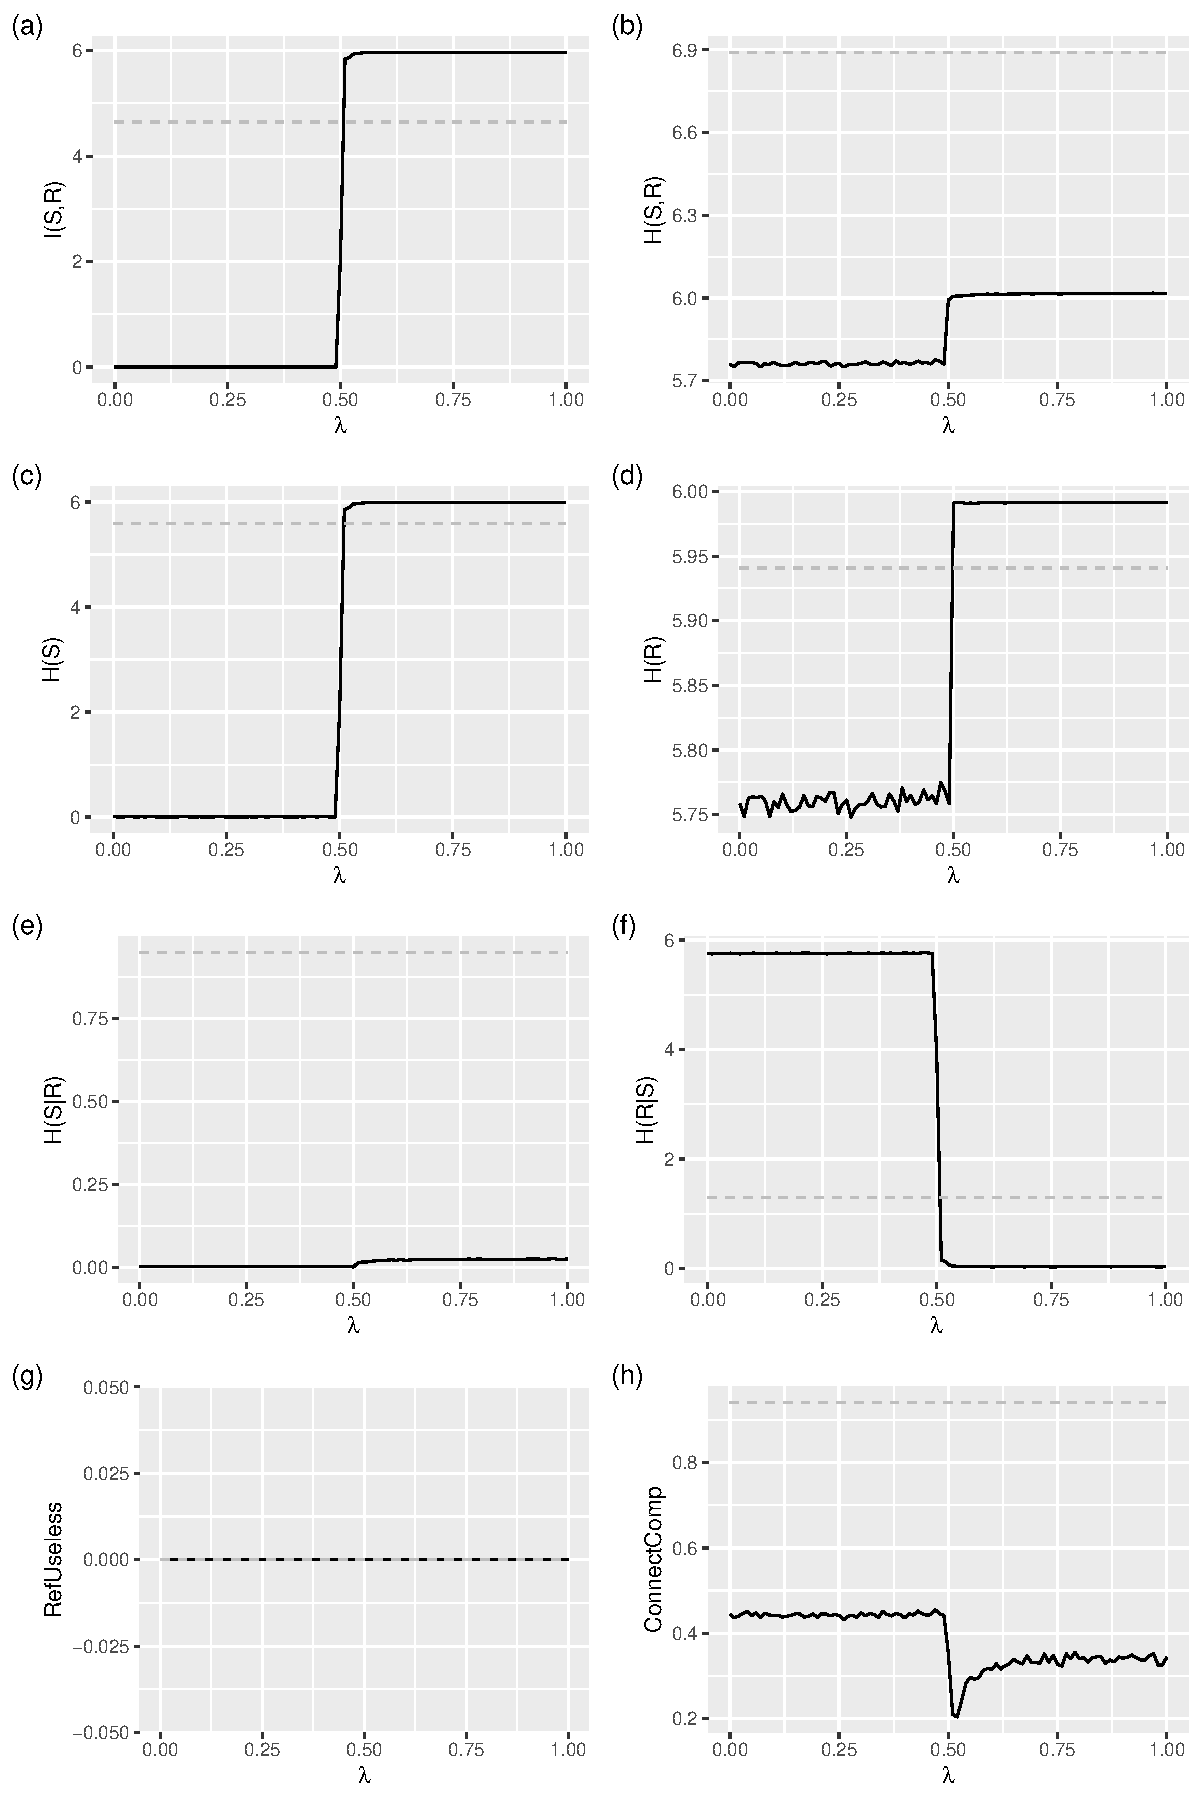
\includegraphics[height=0.7\textheight]{informationTheoretic_uniform_phi1_nm400_dynamic_randomBipartite_allowUnlinked}
  \caption{Same information as in Figure \ref{fig:informationTheoretic_firstModel_phi0_nm400_dynamic_randomBipartite_allowUnlinked} but the graph uses the equations of the \secondmodel{} with $\pi$ following a uniform distribution and with $\phi=1$. Averages over 20 realizations.}
  \label{fig:informationTheoretic_uniform_phi1_nm400_dynamic_randomBipartite_allowUnlinked}
\end{figure}

\begin{figure}
  \centering
  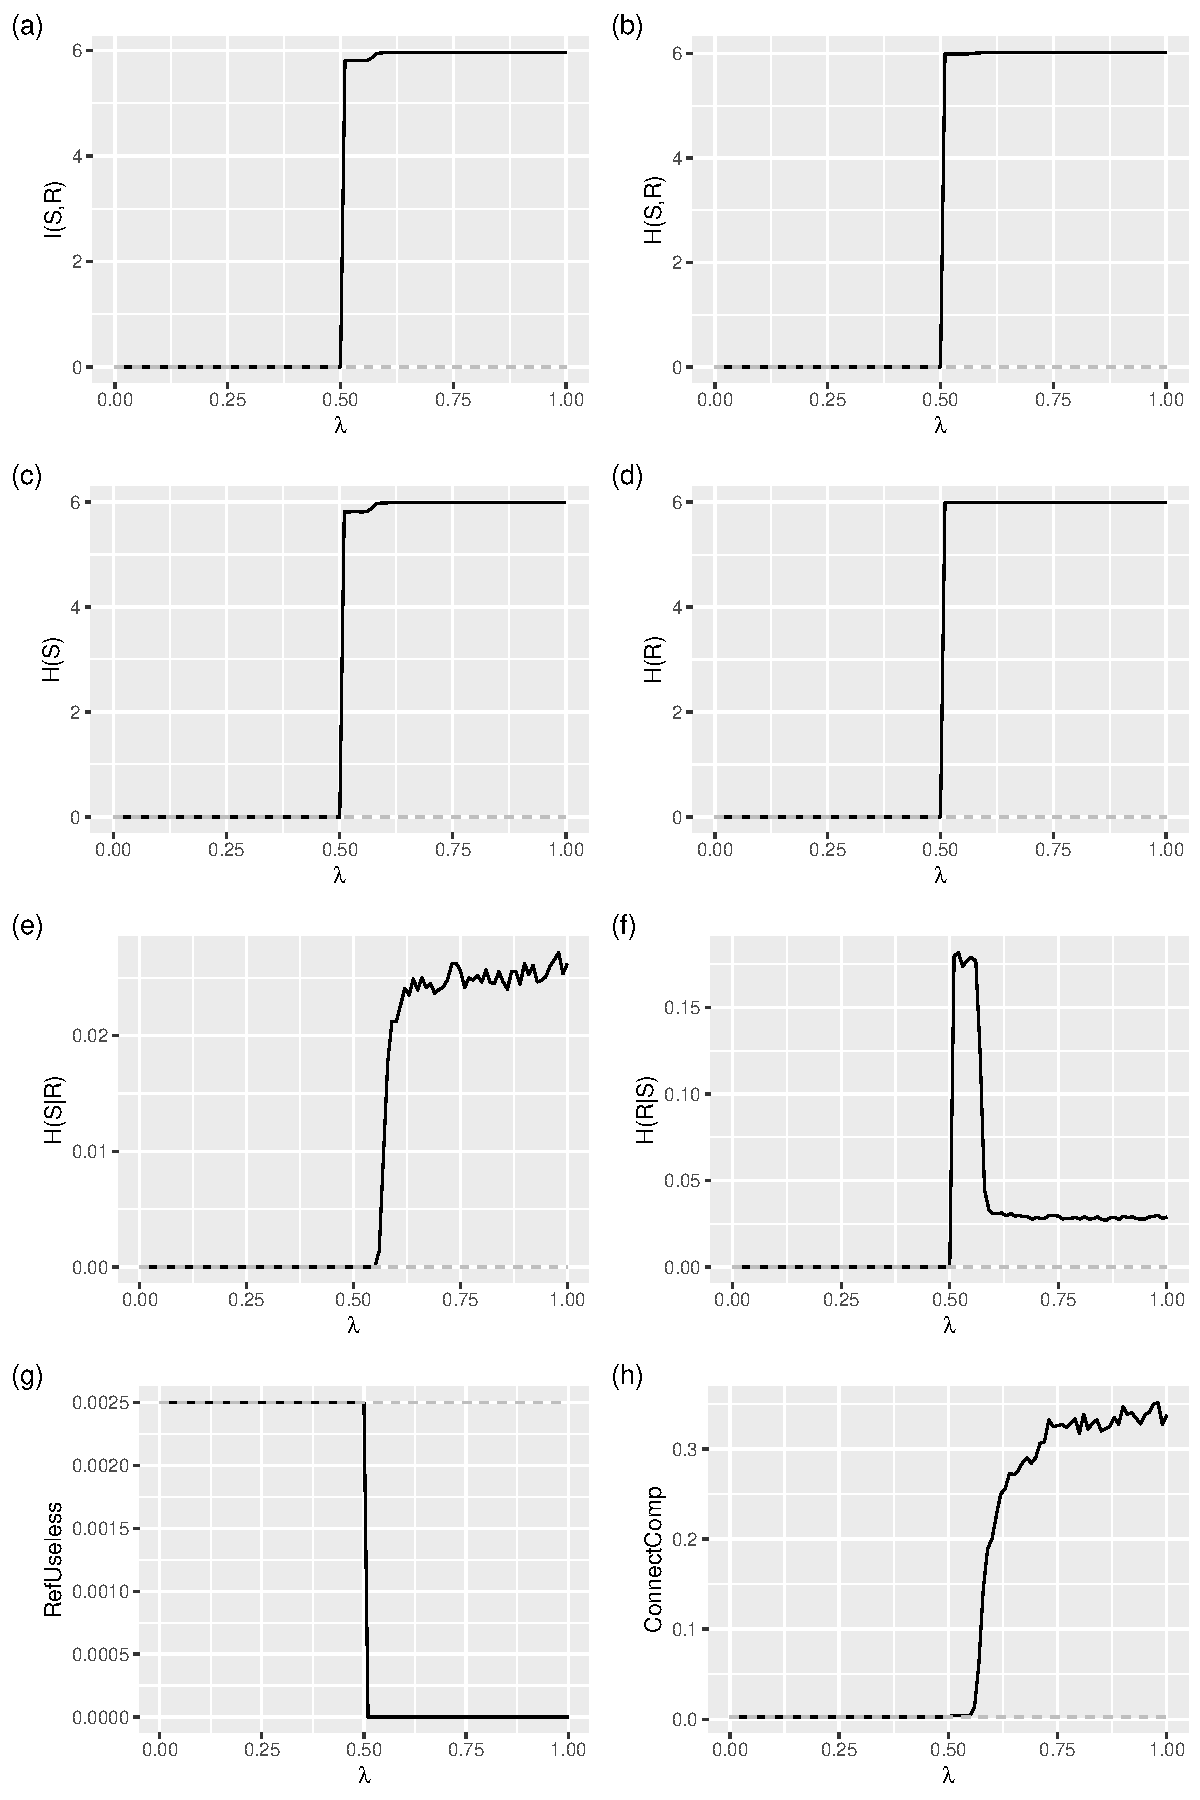
\includegraphics[height=0.7\textheight]{informationTheoretic_uniform_phi1_nm400_dynamic_singleLink_allowUnlinked}
  \caption{Same information as in Figure \ref{fig:informationTheoretic_firstModel_phi0_nm400_dynamic_randomBipartite_allowUnlinked} but the graph uses the equations of the \secondmodel{} with $\pi$ following a uniform distribution with $\pi=1$.
The initial condition is a single link. Averages over 20 realizations.}
  \label{fig:informationTheoretic_uniform_phi1_nm400_dynamic_singleLink_allowUnlinked}
\end{figure}

\begin{figure}
  \centering
  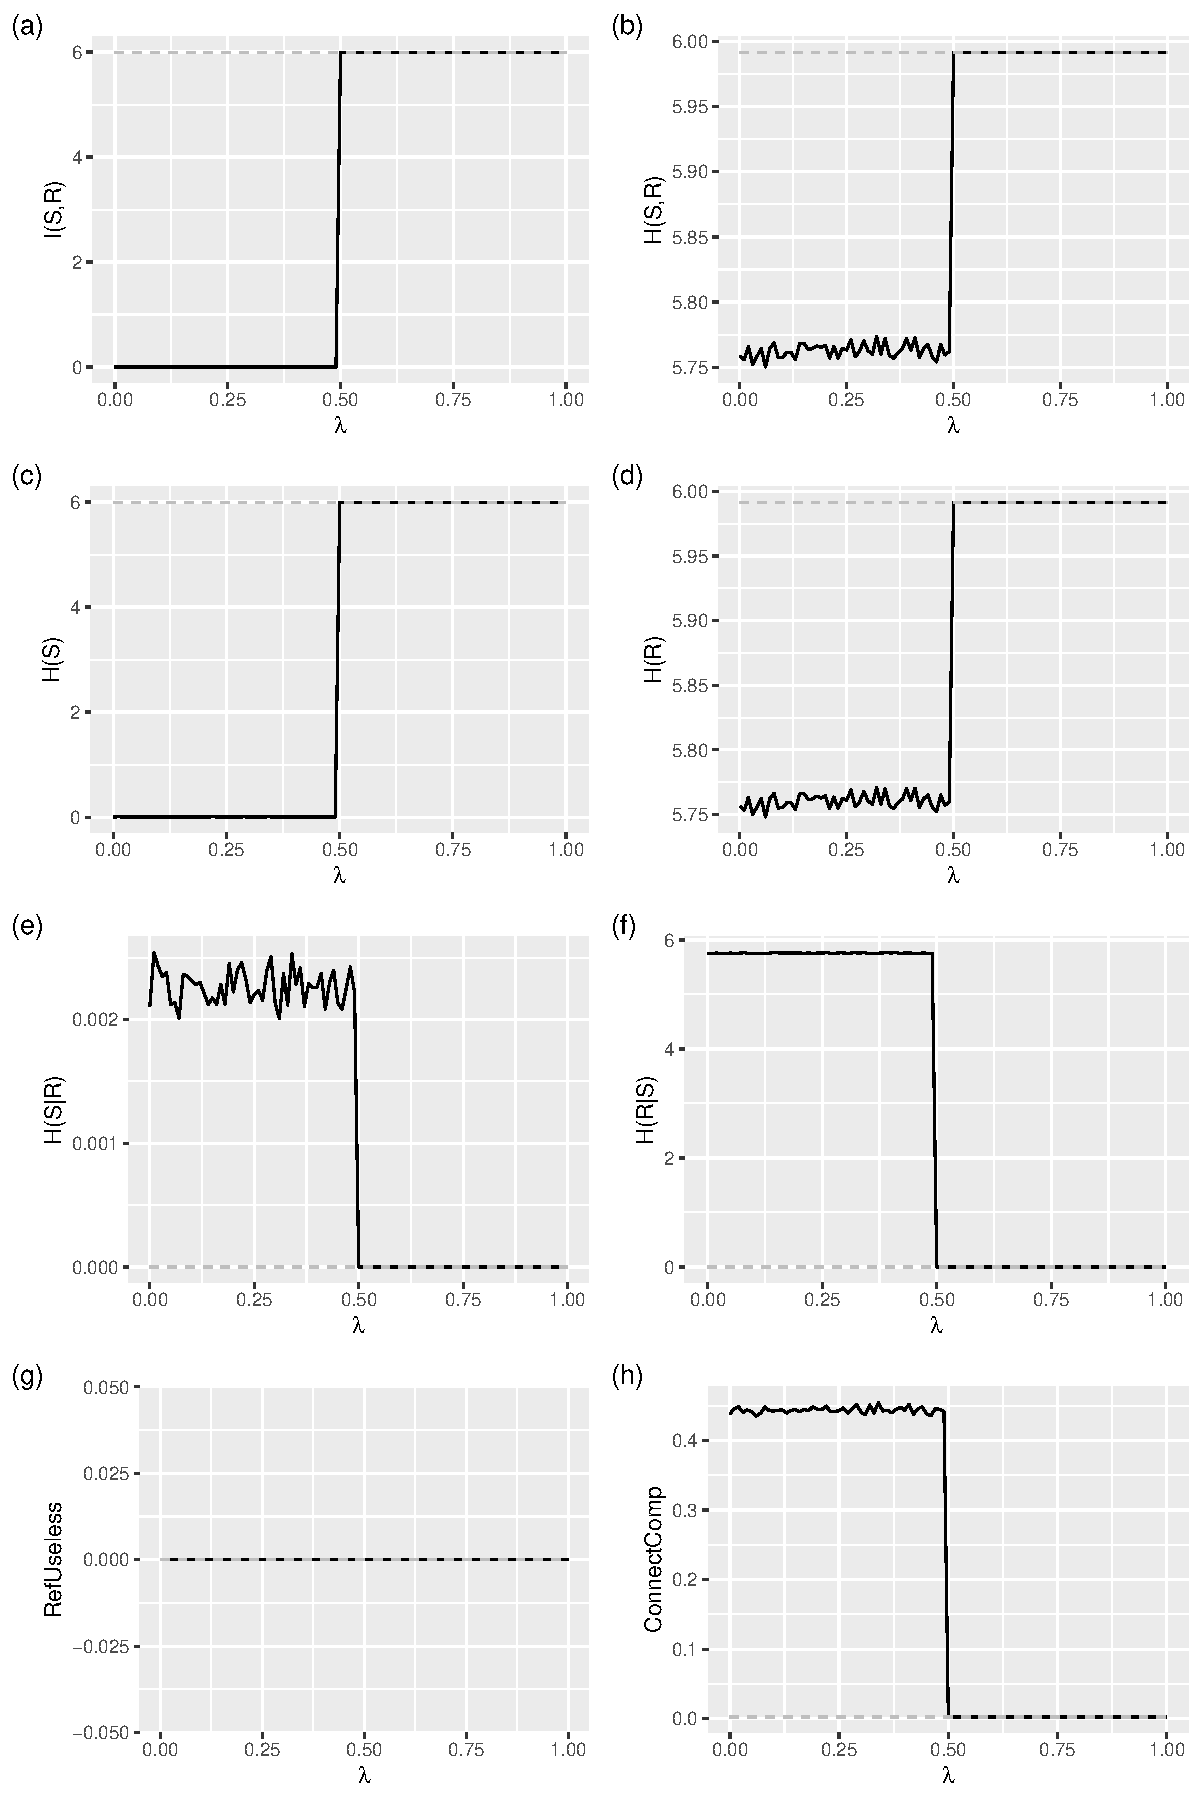
\includegraphics[height=0.7\textheight]{informationTheoretic_uniform_phi1_nm400_dynamic_oneToOne_allowUnlinked}
  \caption{Same information as in Figure \ref{fig:informationTheoretic_firstModel_phi0_nm400_dynamic_randomBipartite_allowUnlinked} but the graph uses the equations of the \secondmodel{} with $\pi$ following a uniform distribution with $\pi=1$.
The initial condition is one to one connections between signals and meanings. Averages over 20 realizations.}
  \label{fig:informationTheoretic_uniform_phi1_nm400_dynamic_oneToOne_allowUnlinked}
\end{figure}

Figures \ref{fig:insideLambda_uniform_phi1_nm400_dynamic_randomBipartite_allowUnlinked} and \ref{fig:insideLambda_uniform_phi1_nm400_dynamic_oneToOne_allowUnlinked} (random and one-to-one respectively) show statistical measures of select values of $\lambda$, with Figures \ref{fig:fitting_insideLambda_uniform_phi1_nm400_dynamic_randomBipartite_allowUnlinked} and \ref{fig:fitting_insideLambda_uniform_phi1_nm400_dynamic_oneToOne_allowUnlinked} (random and one-to-one respectively) showing the fitting of the curve to a power law for a single select value of $\lambda$.
While not very exact, a behavior similar to a power law can be appreciated.
Tables \ref{tab:fitting_insideLambda_uniform_phi1_nm400_dynamic_randomBipartite_allowUnlinked} and \ref{tab:fitting_insideLambda_uniform_phi1_nm400_dynamic_oneToOne_allowUnlinked} (random and one-to-one respectively) show the values of the regression exponent and factor.
As with others, the single link initial condition is not plotted for select values of $\lambda$ as it fails to evolve beyond the single link state.
Appendix \ref{sec:app_figures_second-model} shows the same figures but with disconnected meanings disallowed.

\begin{figure}
  \centering
  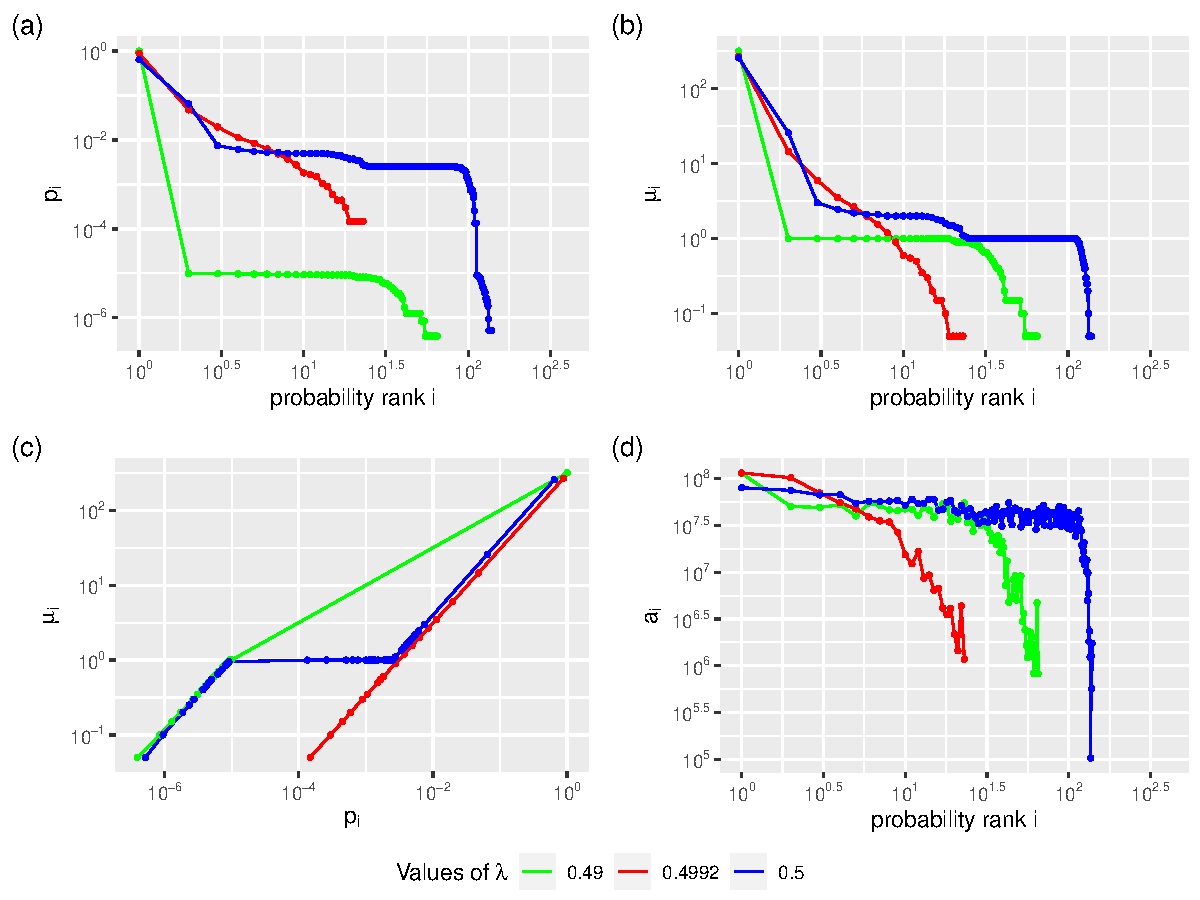
\includegraphics[height=0.7\textheight]{insideLambda_uniform_phi1_nm400_dynamic_randomBipartite_allowUnlinked}
  \caption{Same information as in Figure \ref{fig:insideLambda_firstModel_phi0_nm400_dynamic_randomBipartite_allowUnlinked} but the graph follows the equations of the \secondmodel{} with $\phi=1$ with $\pi$ following a uniform distribution. $\lambda^* = 0.4992$.
  Averages over 20 realizations.}
  \label{fig:insideLambda_uniform_phi1_nm400_dynamic_randomBipartite_allowUnlinked}
\end{figure}

\begin{figure}
  \centering
  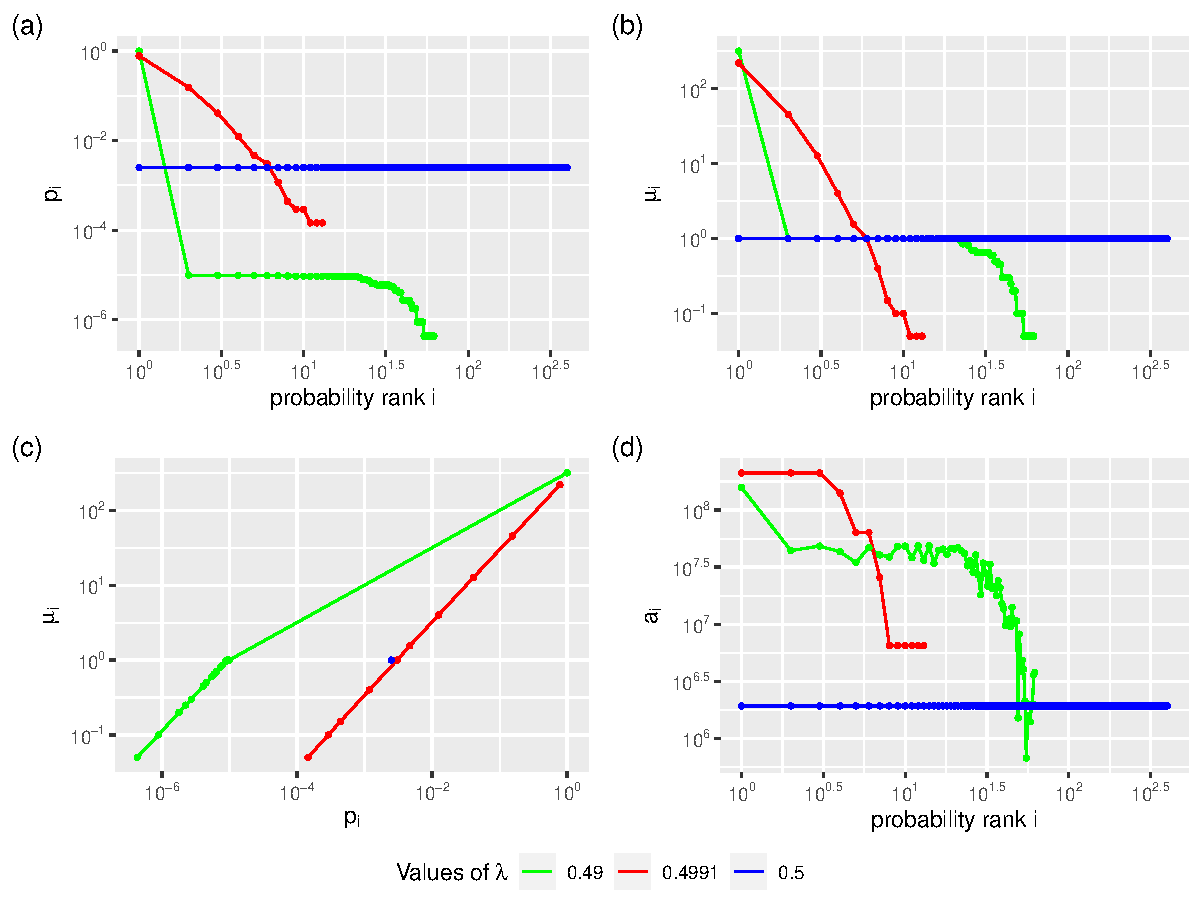
\includegraphics[height=0.7\textheight]{insideLambda_uniform_phi1_nm400_dynamic_oneToOne_allowUnlinked}
  \caption{Same information as in Figure \ref{fig:insideLambda_firstModel_phi0_nm400_dynamic_randomBipartite_allowUnlinked} but the graph follows the equations of the \secondmodel{} with $\pi$ following a uniform distribution and with $\phi=1$. The initial condition is one to one connections between words and meanings. $\lambda^* = 0.4991$.
Averages over 20 realizations.}
  \label{fig:insideLambda_uniform_phi1_nm400_dynamic_oneToOne_allowUnlinked}
\end{figure}

\begin{figure}
  \centering
  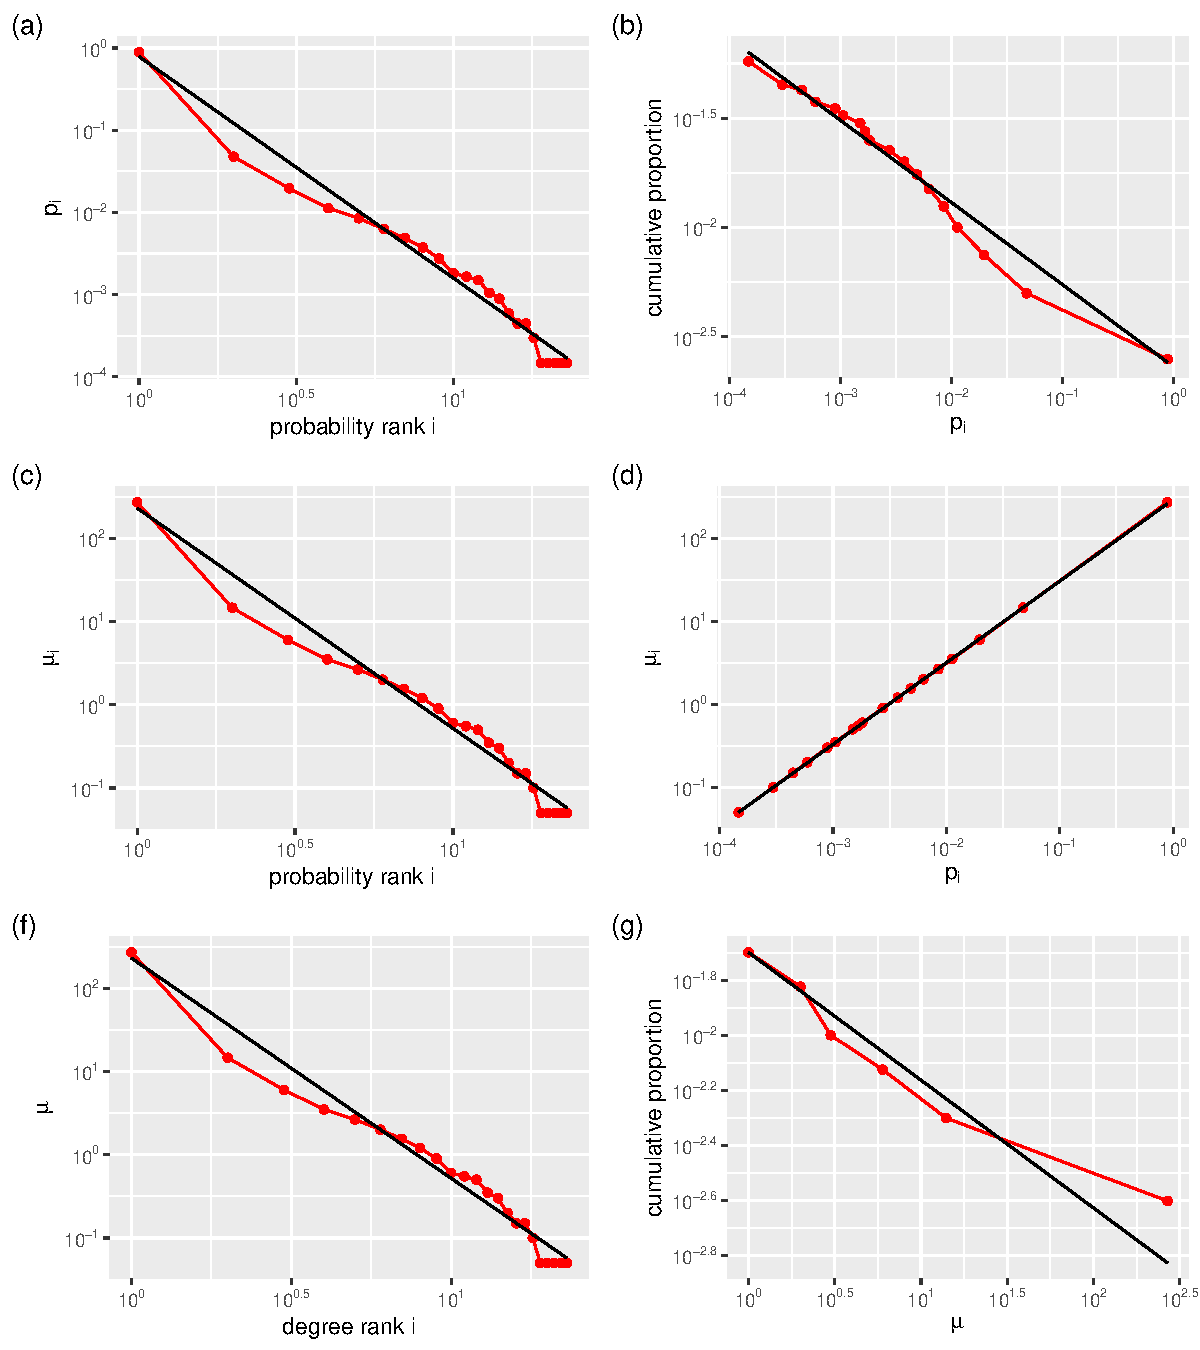
\includegraphics[width=\textwidth]{fitting_insideLambda_uniform_phi1_nm400_dynamic_randomBipartite_allowUnlinked}
  \caption{Same information as in Figure \ref{fig:fitting_insideLambda_firstModel_phi0_nm400_dynamic_randomBipartite_allowUnlinked} but the model follows the equations of the \secondmodel{} with $\pi$ following a uniform distribution and $\phi=1$. $\lambda^*=0.4992$.
Table \ref{tab:fitting_insideLambda_uniform_phi1_nm400_dynamic_randomBipartite_allowUnlinked} shows the values of the exponent and the factor of the fitted power law.}
  \label{fig:fitting_insideLambda_uniform_phi1_nm400_dynamic_randomBipartite_allowUnlinked}
\end{figure}

\begin{figure}
  \centering
  \includegraphics[width=\textwidth]{fitting_insideLambda_uniform_phi1_nm400_dynamic_oneToOne_allowUnlinked}
  \caption{Same information as in Figure \ref{fig:fitting_insideLambda_firstModel_phi0_nm400_dynamic_randomBipartite_allowUnlinked} but the model follows the equations of the \secondmodel{} with $\pi$ following a uniform distribution and $\phi=1$. The initial condition is one to one connections between words and meanings. $\lambda^*=0.4991$.
Table \ref{tab:fitting_insideLambda_uniform_phi1_nm400_dynamic_oneToOne_allowUnlinked} shows the values of the exponent and the factor of the fitted power law.}
  \label{fig:fitting_insideLambda_uniform_phi1_nm400_dynamic_oneToOne_allowUnlinked}
\end{figure}

% latex table generated in R 4.1.1 by xtable 1.8-4 package
% Sun Oct  3 01:17:32 2021
\begin{table}[ht]
\centering
\begin{tabular}{lrr}
  \hline
plot & $\alpha$ & $k$ \\ 
  \hline
a & 2.6942979 & 0.7855283 \\ 
  b & 0.3751754 & 0.0023094 \\ 
  c & 2.6454013 & 229.8644521 \\ 
  d & -0.9825933 & 291.4160609 \\ 
  f & 2.6454013 & 229.8644521 \\ 
  g & 0.4641743 & 0.0200000 \\ 
   \hline
\end{tabular}
\caption{Table showing the exponent and factor of the power laws fitted in Figure \ref{fig:fitting_insideLambda_uniform_phi1_nm400_dynamic_randomBipartite_allowUnlinked}} 
\label{tab:fitting_insideLambda_uniform_phi1_nm400_dynamic_randomBipartite_allowUnlinked}
\end{table}


\begin{table}
  \centering
  \begin{adjustbox}{max width=\textwidth}
    \begin{tabular}{llSS}
      \toprule
      plot & law & $a$ & $k$ \\ 
      \midrule
      a & word frequency & 3.8860954 & 2.27097983 \\ 
      b & \redtxt{word frequency (cumulative)} & 0.2671876 & 0.00303420 \\ 
      c & meaning distribution & 3.8007579 & 632.05935245 \\ 
      d & meaning frequency & -0.9804221 & 293.30509675 \\ 
      f & \redtxt{meaning distribution} & 3.8007579 & 632.05935245 \\ 
      g & \redtxt{meaning distribution (cumulative)} & 0.2924813 & 0.01500000 \\ 
      \bottomrule
    \end{tabular}
  \end{adjustbox}
  \caption{\redtxt{en vermell: cal mostrar?} Table showing the exponent and factor of the power laws fitted in Figure \ref{fig:fitting_insideLambda_uniform_phi1_nm400_dynamic_oneToOne_allowUnlinked}} 
  \label{tab:fitting_insideLambda_uniform_phi1_nm400_dynamic_oneToOne_allowUnlinked}
\end{table}

%%% Local Variables:
%%% mode: latex
%%% TeX-master: "../tfm"
%%% End:


%%% Local Variables:
%%% mode: latex
%%% TeX-master: "tfm"
%%% End:

\chapter{Discussion}
\label{cha:discussion}

In this chapter the results of the thesis are discussed.
Several of the results shown in Chapter \ref{cha:results} are commented and related to the linguistic laws introduced in Chapter \ref{cha:introduction}.
Section \ref{sec:discussion_math} covers this part of the discussion as well as the quantitative linguistics side of the results in general.
A model should be able to make predictions.
Whether this models have been able to make predictions will be discussed.
Section \ref{sec:discussion_comp} discusses the results relating to the computational side.
It focuses specially on the optimization aspects of the model and the local minima of the cost function that may or may not be found by this approach.
Finally, Section \ref{sec:discussion_future-work} talks about possible future work that might stem from this thesis.

\section{Quantitative linguistics discussion}
\label{sec:discussion_math}

Chapter \ref{cha:introduction} already explained several models that have been used to try to explain linguistic laws, such as the random typing model or Simon's model.
However, a distinction must be made between a model that simply describes a phenomenon and one that aims to explain it.
There is no explanation without theory, and theory is a series of principles.
Not all models can give explanations, because they cannot make predictions.

While other models can describe Zipf's law or other power laws, they cannot make predictions beyond that.
One could not use Simon's model to explain how children learn new words while these models can be used to try to make this kind of prediction. \cite{Ferrer2017a} \cite{Carrera2021a}

Here, based on the presented results, we discuss whether these models can explain certain language laws, and how strong this result actually is.

Looking at the effect of the initial conditions, in all cases the single link initial condition failed to evolve.
As seen in Table \ref{tab:summary-initial-condition}, this is a minimum of the cost function when \lambdaZeroToHalf{}.
Here, we see empirically that it is a fixed point of the optimization process.
For \lambdaZeroToHalf{} it remained a single link, while for \lambdaHalfToOne{} it became a one to one bijection between words and meanings. See Figures \ref{fig:informationTheoretic_firstModel_phi0_nm400_dynamic_singleLink_allowUnlinked}, \ref{fig:informationTheoretic_firstModel_phi1_nm400_dynamic_singleLink_allowUnlinked}, \ref{fig:informationTheoretic_uniform_phi0_nm400_dynamic_singleLink_allowUnlinked} and \ref{fig:informationTheoretic_uniform_phi1_nm400_dynamic_singleLink_allowUnlinked}. It can be seen how there is no intermediate stage in the phase change at $\lambda \approx 1/2$.

From a language evolution point of view, it is possible that human language follows a different cost function, one for which a single link initial condition wouldn't fail to become a human language.
However, borrowing the concepts of C.S. Peirce \cite{Atkin2010a}, it can be speculated that languages first developed as random iconic relationships (that is, words were similar to their meaning, for instance the utterance ``bark'' being similar to a dog's barking sound) and as the language evolved (optimized) symbolic relationships began to appear.

\redtxt{It was expected to see the proportion of referentially useless words rise for larger values of $\lambda$ and diminish as $\lambda$ increased.
However, only in the case of a single link graph there is a word considered to be referntially useless, the one that was part of that single edge.
In any other cases there are no referentially useless words.
This could be due to the definition of a referentially useless word (Equation \eqref{eq:referentially-useless-word}).}

\redtxt{It was also expected to see the proportion of vertices belonging to the largest connected component to be significant at least for values of $\lambda$ closer to $\lambda^*$.
While this value does not reach a peak in that case, it does show an interesting behavior in the neighborhood of $\lambda^*$.}

\subsection{Zipf's word frequency laws}
\label{sec:discussion_math_word-freq}

\redtxt{Here we intend to verify Zipf's law of word frequency.
This law as already stated in Equation \eqref{eq:zipf_law} but it is repeated here for clarity,
\begin{equation*}
  f \propto i^{--\alpha}
\end{equation*}
where $f$ is a word's frequency and $i$ its rank.
The exponent $\alpha$ is generally considered to be 1.
However, reality is not as cut and clear.}

\redtxt{While indeed, the exponent has been found to be centered around 1 for English there can be a large variation. \cite{Moreno2016a}
For languages other than English, the value is not necessarily centered around 1, and the variation can be even greater. \cite{Mehri2017a}}

Zipf's law of word frequency can be observed in some form in both the \firstmodel{} and the \secondmodel{}.
Figures \ref{fig:fitting_insideLambda_firstModel_phi0_nm400_dynamic_randomBipartite_allowUnlinked}, \ref{fig:fitting_insideLambda_uniform_phi0_nm400_dynamic_randomBipartite_allowUnlinked} and \ref{fig:fitting_insideLambda_uniform_phi1_nm400_dynamic_randomBipartite_allowUnlinked} show that a power law appears in the frequency-rank relationship plot, subfigure (a).
However, \ref{fig:fitting_insideLambda_firstModel_phi1_nm400_dynamic_randomBipartite_allowUnlinked} does not show a power law.
Instead a single word dominates while the rest are kept at a low frequency.

Previous results had already noted that a power law appeared for the \firstm{} and \secondmodel{} for $\phi=0$ \cite{Ferrer2005a} \cite{Ferrer2003a}.
And while these figures show that a power law appears for a select value of $\lambda$ this does not mean that they cannot appear for others.
Additionally, these figures now show that Zipf's law also appears for an initial condition other than a random bipartite graph.
This makes the previously found prediction even stronger.

As for the values of the power law parameters, they are also similar to the ones found previously.
In \cite{Ferrer2005a} a value of $\alpha \approx 1.5$ is given, which is replicated here in Table \ref{tab:fitting_insideLambda_firstModel_phi0_nm400_dynamic_randomBipartite_allowUnlinked}.
Interestingly, when the initial condition is a one to one graph, $\alpha \approx 4$ (Table \ref{tab:fitting_insideLambda_firstModel_phi0_nm400_dynamic_oneToOne_allowUnlinked}) which is a much higher value.

In \cite{Ferrer2003a}, a power law with $\alpha \approx 1$ was found for the \secondmodel{} when $\lambda=0.41$.
Here, values of $\lambda$ closer to $1/2$ were examined and a power law was still found.
However, the exponent was once again much larger than 1 for both the random bipartite graph and the one to one connections as initial conditions (Tables \ref{tab:fitting_insideLambda_uniform_phi0_nm400_dynamic_randomBipartite_allowUnlinked} and \ref{tab:fitting_insideLambda_uniform_phi0_nm400_dynamic_oneToOne_allowUnlinked}).
%TODO \redtxt{This raises a question, is it possible to find a power law with $\alpha \approx 1$ in the \firstmodel{} for other values of $\lambda$? (posar a future work)}

When $\phi=1$ is added to the \secondmodel{}, $\alpha \approx 2.7$ and $\alpha \approx 3.9$ for the random and one to one initial conditions respectively.

\redtxt{All these exponents are relatively far from the $\alpha \approx 1$ found by Zipf for human language. \cite{Zipf1949a}
However, as one must bear in mind that this value can vary greatly in English, and be outright different in other languages, as seen in the beginning of this section.
This is all to say, the values of $\alpha$ found may not be exactly 1, but neither are the values often found from studies on human language.
Zipf's law can vary greatly in human language \cite{Ferrer2005c} \cite{Baixeries2013a} and the values found here are not that far from what could be considered real values.}

It's also worth noting that the curves shown follow a power law to certain degrees of similarity.
Figure \ref{fig:fitting_insideLambda_uniform_phi1_nm400_dynamic_randomBipartite_allowUnlinked}, for instance, is not perfectly straight in the log-log scale.
While Figure \ref{fig:fitting_insideLambda_firstModel_phi0_nm400_dynamic_randomBipartite_allowUnlinked} follows a line almost perfectly until the last tail of lower rank probabilities which drops drastically.

In summary, while power laws have been found, Zipf's law with a value of $\alpha \approx 1$ is not found, but even for human language that value is not necessarily exact, and the exponents found are not very far from values found in real human languages.

\subsection{Zipf's meaning frequency law}
\label{sec:discussion_math_meaning-freq}

\begin{redenv}
Now we will see how the models can verify Zipf's meaning frequency law, and the relationship between the word frequency, meaning frequency and meaning distribution laws.
In the introduction the word frequency (Equation \eqref{eq:zipf_law}), meaning frequency (Equation \eqref{eq:meaning-frequency-law}) and meaning distribution (Equation \eqref{eq:meaning-distribution-law}) laws were given.
They are reproduced here again for clarity,
\begin{align*}
  f &\propto i^{-\alpha} \\
  \mu &\propto f^\delta \\
  \mu &\propto i^{-\gamma}.
\end{align*}
The relationship between the three exponents was also given in Equation \eqref{eq:relation-exponents}, and is also reproduced here again,
\begin{equation*}
  \delta = \frac{\gamma}{\alpha}.
\end{equation*}
The $\phi$ parameter was added to the model to try and predict Zipf's meaning frequency law
It should be expected that
\begin{equation}
  \label{eq:delta-from-phi}
  \delta = \frac{1}{\phi + 1},
\end{equation}
as seen in previous research. \cite{Ferrer2018a}
For human language, it would be expected that $\delta \approx 1/2$, $\gamma \approx 1/2$ and $\alpha \approx 1$.
\end{redenv}

In the case of the \firstmodel{} with $\phi=0$, power laws are found in subfigures (a), (c) and (d) of Figure \ref{fig:fitting_insideLambda_firstModel_phi0_nm400_dynamic_randomBipartite_allowUnlinked} (random bipartite graph as initial condition) and Figure \ref{fig:fitting_insideLambda_firstModel_phi0_nm400_dynamic_oneToOne_allowUnlinked} (one to one graph as initial condition).
For the random initial condition, $\alpha \approx 1.5$, $\gamma \approx 1.5$ and $\delta \approx 1$ (Table \ref{tab:fitting_insideLambda_firstModel_phi0_nm400_dynamic_randomBipartite_allowUnlinked}). While the relationship from Equation \eqref{eq:relation-exponents} holds, it does not do so with the values of human language ($\alpha=1$, $\gamma=\delta=1/2$).
However, one should remember that these values are not exact and, as seen in Section \ref{sec:discussion_math_word-freq} for $\alpha$, can vary quite a bit; for various languages, within the same language and even depending on specific statistical methodologies.

For the one to one initial condition, $\alpha \approx 4$, $\gamma \approx 4$ and $\delta \approx 1$, the same problem as with the random initial condition but for values even farther away from human language.
When $\phi=1$ is introduced to the first model the power laws disappear, the expected relationship (Equation \eqref{eq:relation-exponents}) does not appear and the value of $\delta$ also is not the expected one (Equation \eqref{eq:delta-from-phi}).

As for the \secondmodel{} with $\phi=0$ the relationships between degree of a word and its probability rank and also between degree of a word and its frequency do not follow power laws (Figure \ref{fig:fitting_insideLambda_uniform_phi0_nm400_dynamic_randomBipartite_allowUnlinked}) for a value of $\lambda$ close to $1/2$.
If using the approximations of a power law obtained from the regression, a value of $\delta \approx 1/2$ is recovered (Table \ref{tab:fitting_insideLambda_uniform_phi0_nm400_dynamic_randomBipartite_allowUnlinked}) however the rest of parameters continue to be far from human language.
When the initial graph is one to one instead of random, power laws are found (Figure \ref{fig:fitting_insideLambda_uniform_phi0_nm400_dynamic_oneToOne_allowUnlinked}) but $\delta \approx 1$.
When adding $\phi=1$ to the \secondmodel{}, $\delta \approx 1$ for both initial conditions, which differs from the value expected from Equation \eqref{eq:delta-from-phi}.

In summary, while the relationship from Equation \eqref{eq:relation-exponents} holds for many of the combinations of parameters tested, values similar to those of human language are not found.
Adding the parameter $\phi=1$ does not seem to help obtain values closer to human language.
Indeed, for the \firstmodel{} it removed the power law behavior.

\subsection{Zipf's age frequency law}
\label{sec:discussion_math_age-freq}

An interesting and somewhat unexpected result is that every single combination of parameters consistently shows Zipf's age frequency law.
This is not explicitly stated as a power law and it does not appear as one in the data.
However, it seems that the correlation always holds for these models: Under any combination of parameters more frequent words are older words.
As seen in Chapter \ref{cha:introduction}, Zipf argued that this should be the case in his book \cite{Zipf1949a} and found empiric data in favor of this (Figure \ref{fig:zipf_word_ages}).

Both models very strongly reflect this law.
Again, it is a consistent tendency in every result obtained, Figures \ref{fig:insideLambda_firstModel_phi0_nm400_dynamic_randomBipartite_allowUnlinked},  \ref{fig:insideLambda_firstModel_phi0_nm400_dynamic_oneToOne_allowUnlinked},  \ref{fig:insideLambda_firstModel_phi1_nm400_dynamic_randomBipartite_allowUnlinked},  \ref{fig:insideLambda_firstModel_phi1_nm400_dynamic_oneToOne_allowUnlinked},  \ref{fig:insideLambda_uniform_phi0_nm400_dynamic_randomBipartite_allowUnlinked},  \ref{fig:insideLambda_uniform_phi0_nm400_dynamic_oneToOne_allowUnlinked},  \ref{fig:insideLambda_uniform_phi1_nm400_dynamic_randomBipartite_allowUnlinked} and \ref{fig:insideLambda_uniform_phi1_nm400_dynamic_oneToOne_allowUnlinked}.

This correlation is one of the main results of this thesis.
\redtxt{The initial models with $\phi=0$ are able to reproduce more real linguistic laws than previously thought.
As seen in Table \ref{tab:comparison_models}, the simpler models with $\phi=0$ end up reproducing more laws than the \firstmodel{} with $\phi \neq 0$.
Furthermore, the age frequency law is observed to be a trend followed by all the obtained results.
However, it is not an obvious direct consequence of the formulation of the model.
The fact that model reproduces this linguistic law without attempting to formulate it specifically to try to replicate it speaks to the quality of this model for language.
This is specially interesting when seeing table \ref{tab:summary-computational}, which shows that the simpler models are computationally less complex too.
}

\section{Computational results discussion}
\label{sec:discussion_comp}

At the core of this model is the minimization of a cost function.
This cost function is used to describe the effort of speaker and hearer of the language.
For the \firstmodel{}, this cost function has shown to be able to predict a bias in child vocabulary learning. \cite{Ferrer2017a} \cite{Carrera2021a}

\subsection{Local minima}
\label{sec:discussion_comp_minima}

For some combinations of parameters it is clear that a minima has been reached.
This is the case when the extreme states (a single link, a one to one relationship of words and meanings) are achieved in the graph.
In other cases it is not so clear that a local minima has actually been reached.
This includes the cases studied in Chapter \ref{cha:results} with $\lambda^*$ where linguistic laws could be recovered.
The stronger the stop condition of the minimization algorithm, the more sure one can be that a minimum has been reached.
However, this also means a longer time to obtain a result.

\subsection{Dependency on initial condition}
\label{sec:discussion_comp_initial-condition}

The optimization process has been carried out for different initial conditions.
It is clear that there is a dependence on the initial condition.
When the initial condition is a single link the system fails to evolve into a configuration where language laws can be reproduced.
The single link configuration, which was already found to be a minimum for $\Omega(\lambda)$ for \lambdaZeroToHalf{}, seems to be a fixed point of the simulation during that interval.
The one to one configuration also seems to be a fixed point for the interval for which it is a minimum of the cost function, \lambdaHalfToOne{}.
It's also apparent that the one to one configuration has less words with nonzero probability than the random configuration for $\lambda=\lambda^*$.
The mathematical work required to prove that these two conditions are indeed fixed points of the simulation is no present in this thesis.

No results are presented for the complete initial condition beyond some sample optimized graphs.
This is due to the runtime of the simulation for larger values of $n$ and $m$.
Similarly, there is no variation of the density of the random initial conditions seen.

\section{Future work}
\label{sec:discussion_future-work}

Much work could be further derived from the contributions presented here.
Parameters could be tweaked and changed to observe various versions of the models and try to more closely obtain linguistic laws.
But the more fundamental ideas presented could also be changed to improve the results and or to use different algorithms that might be more efficient and present less numerical error.

\subsection{Optimization methods}
\label{sec:discussion_future-work_optimization}

The model is optimized by performing mutations on the boolean values of the $A$ adjacency matrix of the graph using a Monte Carlo Markov Chain method at zero temperature.

An alternative to this is simulated annealing.
That is, to use nonzero temperature for the Monte Carlo process, allowing for non optimal states to be chosen.
This might help escape from states that are not local minima but that also have very few paths to other minimal states.
This would only need to slightly modify the optimization algorithm to add the temperature parameter.

Another alternative optimization method is gradient descent.
The cost function could be optimized as a function of $A$ (with $\lambda$ being a constant) $\Omega(A)$ would then need to be derivable.
A first step to make it derivable would mean making $A$ a matrix of reals representing weights instead of booleans representing just whether the connection exists or not.
This would be a much more complex endeavor than simulated annealing.
However, this would result in the use of a method similar to what is used in AI with a much lower complexity than the models seen in AI.

\redtxt{Another optimization worth considering is a genetic algorithm with a population of random matrices which are selected and recombined according to some parameters.}

\subsection{Other values of $\phi$}
\label{sec:discussion_future-work_phi}

Other values of $\phi$ can be explored.
Here only values of $\phi$ 0 or 1 are seen.
Other interesting values that have not been studied in depth are 0.5 and 1.5.

This would be a very simple thing to implement, as easy as changing a configuration file (see Appendix \ref{sec:app_code_program-parameters}).

\subsection{Vocabulary learning}
\label{sec:discussion_future-work_vocabulary-learning}

The \firstmodel{} has already been used to predict vocabulary learning biases in children, both for the case $\phi=0$ \cite{Ferrer2017a} and for $\phi=1$ \cite{Carrera2021a}.
A similar analysis could be done for the \secondmodel{}.
Can it make these predictions? Under which conditions? This is purely mathematical work, without any computational aspects to it.

\subsection{Numerical error}
\label{sec:discussion_future-work_numerical-error}

A great effort to find ways to reduce numerical error due to floating point arithmetic has been done as part of this thesis.
However this can continue to be a problem, specially for higher values of $n$ and $m$ where a greater number of additions and subtractions take place.
It is possible that some dynamic calculations can be done statically without sacrificing efficiency.
Indeed, some variables are already calculated statically in the dynamic algorithm, as they have similar complexity in either case but involve many more additions and subtractions in the dynamic algorithm.
A similar effort could be done for other sections of the dynamic computations.

\subsection{\redtxt{Further computational optimizations (NOU)}}
\label{sec:discussion_future-work_comp-opt}

While care was taken to try to optimize the actual computations, it is possible that they could be further improved.
Either by making improvements to the code or by conceptual changes on a higher level.
The goal of such changes should be to make initial conditions with more edges (such as a complete bipartite graph) possible, reducing their current prohibitive computational cost.

%%% Local Variables:
%%% mode: latex
%%% TeX-master: "tfm"
%%% End:


\appendix

\chapter{Codi}
\begin{itemize}
\item afegir repositori amb el codi
\end{itemize}

%%% Local Variables:
%%% mode: latex
%%% TeX-master: "tfm"
%%% End:

\chapter{Formulae}
\label{cha:app_formulae}

\redtxt{derivacions llargues i pagines i pagines de mates van aqui}

\section{Simplification of the equations of entropies}
\label{sec:app_formulae_trick}

Equation \eqref{eq:definition-trick} is used in several parts of the thesis to simplify the expressions of entropies.
The derivation is short, but it is not added into the main text of the thesis for the sake of clarity and focus.

\begin{align*}
              -\sum_i & \frac{x_i}{T} \log\frac{x_i}{T} \\
  -\frac{1}{T} \sum_i & x_i \log x_i - x_i \log T \\
  -\frac{1}{T} \sum_i & x_i \log x_i + \log(T) \frac{1}{T} \sum_i x_i \\
\end{align*}
at this point we can apply
\begin{equation*}
  \sum_i x_i = T
\end{equation*}
and obtain
\begin{align*}
  \log T - \frac{1}{T} \sum_i & x_i \log x_i\\
\end{align*}

\section{Derivation of the joint entropy in the \secondmodel}
\label{sec:app_formulae_join-entropy_second-model}

In Section \ref{sec:model_math_second-model} the derivation of the joint entropy is left as just the high level reasoning of which formulas may be used to obtain its expression.
Here, the full derivation of both approaches is given.

The first approach consists of applying Equation \eqref{eq:definition-join-prob_second-model} to the information theory definition of $H(S,R)$ (Equation \eqref{eq:definition-HSR}),
\begin{align*}
  H(S,R) =& - \sum_{i=1}^n \sum_{j=1}^m p(s_i, r_j) \log \left[ p(s_i, r_j) \right] \\
         =& - \sum_{i=1}^n \sum_{j=1}^m \frac{a_{i,j} (1 - \delta_{\omega_j,0}) \mu_i^\phi \pi(r_j)}{\rho \omega_{\phi,j}} \log \left[ \frac{a_{i,j} (1 - \delta_{\omega_j,0}) \mu_i^\phi \pi(r_j)}{\rho \omega_{\phi,j}} \right] \\
         =& - \frac{1}{\rho} \sum_{i=1}^n \sum_{j=1}^m \frac{a_{i,j} (1 - \delta_{\omega_j,0}) \mu_i^\phi \pi(r_j)}{\omega_{\phi,j}} \log \left[ \frac{\mu_i^\phi \pi(r_j)}{\rho \omega_{\phi,j}} \right] \\
         =& - \frac{1}{\rho} \sum_{j=1}^m \frac{(1 - \delta_{\omega_j,0}) \pi(r_j)}{\omega_{\phi,j}} \Bigg[ \phi \sum_{i=1}^n a_{i,j} \mu_i^\phi \log \mu_i \\
          & + \log \pi(r_j) \sum_{i=1}^n a_{i,j} \mu_i^\phi - \log(\rho) \sum_{i=1}^n a_{i,j} \mu_i^\phi \\
          & - \log(\omega_{\phi,j}) \sum_{i=1}^n a_{i,j} \mu_i^\phi \Bigg].
\end{align*}
Applying Equation \eqref{eq:definition-nu} we arrive at Equation \eqref{eq:definition-HSR_second-model}.

The second approach consists on using other less complex expressions we have available and building up from them using the definitions
\begin{align}
  \label{eq:definition-HSR_appendix}
  H(S,R) &= H(S|R) + H(R), \\
  \label{eq:definition-HSgR_appendix}
  H(S|R) &= \sum_{j=1}^m H(S|r_j)p(r_j), \\
  \label{eq:definition-HSgrj_appendix}
  H(S|r_j) &= -\sum_{i=1}^n p(s_i|r_j) \log p(s_i|r_j).
\end{align}

Starting from Equation \eqref{eq:definition-HSgrj_appendix} and applying Equation \eqref{eq:definition-cond-prob_second-model} we obtain
\begin{align*}
  H(S|r_j) =& -\sum_{i=1}^n \frac{a_{i,j} \mu_i^\phi \pi(r_j)}{\rho \omega_{\phi,j}} \log \left( \frac{a_{i,j} \mu_i^\phi \pi(r_j)}{\rho \omega_{\phi,j}} \right) \\
           =& \log \omega_{\phi,j} - \frac{1}{\omega_{\phi,j}} \sum_{i=1}^n a_{i,j} \mu_i^\phi \log(a_{i,j} \mu_i^\phi) \\
           =& \log \omega_{\phi,j} - \frac{\phi}{\omega_{\phi,j}} \sum_{i=1}^n a_{i,j} \mu_i^\phi \log(\mu_i)
\end{align*}
and after applying Equation \eqref{eq:definition-nu}
\begin{equation}
  \label{eq:definition-HSgrj_appendix-step}
  H(S|r_j) = \log \omega_{\phi,j} - \frac{\phi \nu_j}{\omega_{\phi,j}}.
\end{equation}

Applying Equations \eqref{eq:definition-HSgrj_appendix-step} and \eqref{eq:definition-prj_second-model} to Equation \eqref{eq:definition-HSgR_appendix} we reach
\begin{align}
  H(S|R) =& \sum_{j=1}^m \left(\log \omega_{\phi,j} - \frac{\phi \nu_j}{\omega_{\phi,j}}\right) \frac{(1 - \delta_{w_j,0}) \pi(r_j)}{\rho} \nonumber \\
  \label{eq:definition-HSgR_appendix-step}
       =& \frac{1}{\rho} \sum_{j=1}^m (1 - \delta_{w_j,0}) \pi(r_j) \left[ \log(\omega_{\phi,j}) - \frac{\phi \nu_j}{\omega_{\phi,j}} \right].
\end{align}

The last step consists of applying Equations \eqref{eq:definition-HSgR_appendix-step} and \eqref{eq:definition-HR_second-model} to Equation \eqref{eq:definition-HSR_appendix}, obtaining Equation \eqref{eq:definition-HSR_second-model} again
\begin{align*}
  H(S,R) &= \frac{1}{\rho} \sum_{j=1}^m (1 - \delta_{w_j,0}) \pi(r_j) \left[ \log(\omega_{\phi,j}) - \frac{\phi \nu_j}{\omega_{\phi,j}} \right] \\
       &+ \log \rho - \frac{1}{\rho} \sum_{j=1}^m (1 - \delta_{w_j,0}) \pi(r_j) \log \pi(r_j) \\
       &= \log \rho - \frac{1}{\rho} \sum_{j=1}^m (1 - \delta_{w_j,0}) \pi(r_j) \left[ \frac{\phi \nu_j}{\omega_{\phi,j}} + \log \frac{\pi(r_j)}{\omega_{\phi,j}} \right].
\end{align*}

\section{Proof that $\sum_{i=1}^n \mu_i^\phi \chi_i = \rho$}
\label{sec:app_formulae_proof-sum-HS_second-model}

In order to use Equation \eqref{eq:definition-trick} in order to simplify the derivation of Equation \eqref{eq:definition-HS_second-model}, it must hold that $\sum_{i=1}^n \mu_i^\phi \chi_i = \rho$.
Here it is shown that this is the case.

Starting from the equality, we can expand both sides
\begin{align*}
\sum_{i=1}^n \mu_i^\phi \chi_i =& \rho \\
\sum_{i=1}^n \mu_i^\phi \sum_{j=1}^m \frac{a_{ij} (1 - \delta_{\omega_j,0}) \pi(r_j)}{\omega_{\phi,j}} =& \sum_{j=1}^m (1 - \delta_{\omega_j,0}) \pi(r_j) \\
\sum_{j=1}^m \left( \sum_{i=1}^n a_{ij} \mu_i^\phi \right) \frac{(1 - \delta_{\omega_j,0}) \pi(r_j)}{\omega_{\phi,j}} =& \sum_{j=1}^m (1 - \delta_{\omega_j,0}) \pi(r_j), \\
\end{align*}
applying Equation \eqref{eq:definition-omegaphi} we obtain
\begin{equation*}
  \sum_{j=1}^m (1 - \delta_{\omega_j,0}) \pi(r_j)
\end{equation*}
on both sides.

Recall the definition of $p(s_i)$ in Equation \eqref{eq:definition-psi_second-model} to see that
\begin{equation*}
  \sum_{i=1}^n p(s_i) = 1
\end{equation*}
immediately follows.

\section{Dynamic Equations for the \secondmodel{}}
\label{sec:app_formulae_dynamic-equations_second-model}

The full derivation of the dynamic equations for the \secondmodel{} is given in this section.
The equations themselves as well as other definitions used here are already given in Section \ref{sec:model_math_second-model}.

In this section, the derivation is logical rather than mathematical, consisting of explanations behind the logic of the equations.

$\rho$ (see Equation \eqref{eq:definition-rho}) only changes when, as a result of the mutation, the meaning $r_j$ either was connected and becomes disconnected or was disconnected and becomes connected, resulting in Equation \eqref{eq:definition-rho_dynamic}.

$\nu_l$ is very similar to $\omega_{\phi,l}$ (compare Equations \eqref{eq:definition-nu} and \eqref{eq:definition-omegaphi}).
Equation \eqref{eq:definition-nu_dynamic} shows how $\nu_l$ changes in the same cases and in the same way as $\omega_{\phi,l}$ (Equation \eqref{eq:definition-wphik_dynamic}).

$\chi_k$ depends on  $\omega_{\phi,l}$ such that $l \in \Gamma_S(k)$ (see Equation \eqref{eq:definition-chi_second-model}).
For $\chi_i$, the entire value has to be recalculated, as every $\omega_{\phi,l}$ for $l \in \Gamma_S(k)$ will have changed (Equation \eqref{eq:definition-wphik_dynamic}).
It is more efficient (and reduces the amount of floating point error) to calculate $\chi_i$ statically than to subtract every $\omega_{\phi,l}$ and then add every $\omega'_{\phi,l}$.
For all other values of $\chi_k$ ($k \neq i$), the affected $\omega_{\phi,l}$ are the intersection of the set of neighbors of $i$ plus the meaning $r_j$ and the set of neighbors of $k$. This is the set $A_{i,j}(k)$ defined in Equation \eqref{eq:definition-A_second-model}. With this reasoning we reach the formula for the dynamic recalculation of $\chi_k$, Equation \eqref{eq:definition-chi_dynamic}.

$X(R)$ (Equation \eqref{eq:definition-XR_second-model}) changes in a very similar way to $\rho$ (Equation \eqref{eq:definition-rho}), as they both depend on the same variable in the same way: only when the meaning $r_j$ becomes connected or disconnected does $X(R)$ change, resulting in Equation \eqref{eq:definition-rho_dynamic}.

$X(S,R)$ (Equation \eqref{eq:definition-XSR_second-model}) will change when a $x(r_l)$ (Equation \eqref{eq:definition-xrj_second-model}) changes.
Both $\omega_{\phi,l}$ and $\nu_l$ change for $l \in \Gamma_S(i) \cup \{j\}$ (Equations \eqref{eq:definition-wphik_dynamic} and \eqref{eq:definition-nu_dynamic}).
So these are the components $x(s_l)$ of $H(S,R)$ that will change.
For the special case of $l=j$ we should not subtract the old value when $r_j$ has become connected as a result of the mutation (as that component was not present), and we should not add the new value when $r_j$ has become disconnected (as that component should not be present).
Or in other words, only subtract the old value if $r_j$ was connected before the mutation (this serves to either update it or to remove it) and only add the new value if $r_j$ is connected after the mutation (this serves to either update it or to add it).
The resulting expression for $X'(S,R)$ is in Equation \eqref{eq:definition-XSR_second-model_dynamic}.

$X(S)$ (Equation \eqref{eq:definition-XS_second-model}) will change when $x(s_k)$ (Equation \eqref{eq:definition-xsi_second-model}) changes, which depends on $\chi_k$ (Equation \eqref{eq:definition-chi_dynamic}).
$\chi_k$ is updated for every $k$ such that $|A_k| \neq \emptyset$ and $\chi_i$ is always updated, which is the definition of the $B_{i,j}(k)$ set (Equation \eqref{eq:definition-B_second-model}).
Using $B_{i,j}(k)$ we obtain the expression for $X'(S)$ in Equation \eqref{eq:definition-XS_second-model_dynamic}.

%%% Local Variables:
%%% mode: latex
%%% TeX-master: "tfm"
%%% End:

\chapter{Figures}
\label{cha:app_figures}

\redtxt{figures que sobren}

\section{Figures of disconnected meanings for the \secondmodel{}}
\label{sec:app_figures_second-model}

Section \ref{sec:results_new_other} shows the results obtained for the current model.
For comparison with \cite{Ferrer2003a}, figures generated from the same sets of parameters as for the \secondmodel{}  but with disconnected meanings kept disallowed are shown here.
The single connection initial state is never shown, as it is an invalid configuration.

For the case $\phi=0$, Figures \ref{fig:informationTheoretic_uniform_phi0_nm400_dynamic_randomBipartite_disallowUnlinked} and \ref{fig:informationTheoretic_uniform_phi0_nm400_dynamic_oneToOne_disallowUnlinked} show the information theoretical measures of the optimal graph for values of $\lambda$ ranging from 0 to 1. They correspond to the initial graph being a random bipartite graph and a one to one configuration respectively.

\begin{figure}
  \centering
  \includegraphics[width=\textwidth]{informationTheoretic_uniform_phi0_nm400_dynamic_randomBipartite_disallowUnlinked}
  \caption{Same information as in Figure \ref{fig:informationTheoretic_uniform_phi0_nm400_dynamic_randomBipartite_allowUnlinked} but disconnected meanings are disallowed.}
  \label{fig:informationTheoretic_uniform_phi0_nm400_dynamic_randomBipartite_disallowUnlinked}
\end{figure}

\begin{figure}
  \centering
  \includegraphics[width=\textwidth]{informationTheoretic_uniform_phi0_nm400_dynamic_oneToOne_disallowUnlinked}
  \caption{Same information as in Figure \ref{fig:informationTheoretic_uniform_phi0_nm400_dynamic_oneToOne_allowUnlinked} but disconnected meanings are disallowed.}
  \label{fig:informationTheoretic_uniform_phi0_nm400_dynamic_oneToOne_disallowUnlinked}
\end{figure}

Figures \ref{fig:insideLambda_uniform_phi0_nm400_dynamic_randomBipartite_disallowUnlinked} and \ref{fig:insideLambda_uniform_phi0_nm400_dynamic_oneToOne_disallowUnlinked} (random and one to one respectively) show statistical measures for select values of $\lambda$, with figures \ref{fig:fitting_insideLambda_uniform_phi0_nm400_dynamic_randomBipartite_disallowUnlinked} and \ref{fig:fitting_insideLambda_uniform_phi0_nm400_dynamic_oneToOne_disallowUnlinked} showing the fitting of the curve to a power law for a select value of $\lambda$.
None of the studied values of $\lambda$ between 0.49 and 0.5 resulted in a power law.
Tables \ref{tab:fitting_insideLambda_uniform_phi0_nm400_dynamic_randomBipartite_disallowUnlinked} and \ref{tab:fitting_insideLambda_uniform_phi0_nm400_dynamic_oneToOne_disallowUnlinked} show the values of the regression's exponent and factor

\begin{figure}
  \centering
  \includegraphics[width=\textwidth]{insideLambda_uniform_phi0_nm400_dynamic_randomBipartite_disallowUnlinked}
  \caption{Same information as in Figure \ref{fig:insideLambda_uniform_phi0_nm400_dynamic_randomBipartite_allowUnlinked} but disconnected meanings are disallowed.}
  \label{fig:insideLambda_uniform_phi0_nm400_dynamic_randomBipartite_disallowUnlinked}
\end{figure}

\begin{figure}
  \centering
  \includegraphics[width=\textwidth]{insideLambda_uniform_phi0_nm400_dynamic_oneToOne_disallowUnlinked}
  \caption{Same information as in Figure \ref{fig:insideLambda_uniform_phi0_nm400_dynamic_oneToOne_allowUnlinked} but disconnected meanings are disallowed.}
  \label{fig:insideLambda_uniform_phi0_nm400_dynamic_oneToOne_disallowUnlinked}
\end{figure}

\begin{figure}
  \centering
  \includegraphics[width=\textwidth]{fitting_insideLambda_uniform_phi0_nm400_dynamic_randomBipartite_disallowUnlinked}
  \caption{Same information as in Figure \ref{fig:fitting_insideLambda_uniform_phi0_nm400_dynamic_randomBipartite_allowUnlinked} but disconnected meanings are disallowed.
Table \ref{tab:fitting_insideLambda_uniform_phi0_nm400_dynamic_randomBipartite_disallowUnlinked} shows the values of the exponent and the factor of the fitted power law.}
  \label{fig:fitting_insideLambda_uniform_phi0_nm400_dynamic_randomBipartite_disallowUnlinked}
\end{figure}

\begin{figure}
  \centering
  \includegraphics[width=\textwidth]{fitting_insideLambda_uniform_phi0_nm400_dynamic_oneToOne_disallowUnlinked}
  \caption{Same information as in Figure \ref{fig:fitting_insideLambda_uniform_phi0_nm400_dynamic_oneToOne_allowUnlinked} but disconnected meanings are disallowed.
Table \ref{tab:fitting_insideLambda_uniform_phi0_nm400_dynamic_oneToOne_disallowUnlinked} shows the values of the exponent and the factor of the fitted power law.}
  \label{fig:fitting_insideLambda_uniform_phi0_nm400_dynamic_oneToOne_disallowUnlinked}
\end{figure}

% latex table generated in R 4.1.1 by xtable 1.8-4 package
% Tue Oct  5 00:38:21 2021
\begin{table}[ht]
\centering
\begin{tabular}{lrr}
  \hline
plot & $\alpha$ & $k$ \\ 
  \hline
a & 5.1239660 & 1744404.5869742 \\ 
  b & 0.1949778 & 0.0413557 \\ 
  c & 1.5237337 & 1164.4863367 \\ 
  d & -0.5072076 & 52.8958272 \\ 
  f & 1.5439705 & 1287.7147444 \\ 
  g & 0.8441915 & 0.2950000 \\ 
   \hline
\end{tabular}
\caption{Table showing the exponent and factor of the power laws fitted in Figure \ref{fig:fitting_insideLambda_uniform_phi0_nm400_dynamic_randomBipartite_disallowUnlinked}} 
\label{tab:fitting_insideLambda_uniform_phi0_nm400_dynamic_randomBipartite_disallowUnlinked}
\end{table}


\begin{table}
  \centering
  \begin{adjustbox}{max width=\textwidth}
    \begin{tabular}{llSS}
      \toprule
      plot & law & $a$ & $k$ \\ 
      \midrule
      a & word frequency & 1.6856845 & 5.9091866 \\ 
      b & \redtxt{word frequency (cumulative)} & 0.5677904 & 0.0082092 \\ 
      c & meaning distribution & 1.6856845 & 2363.6746229 \\ 
      d & meaning frequency & -1.0000000 & 400.0000000 \\ 
      f & \redtxt{meaning distribution} & 1.6856845 & 2363.6746229 \\ 
      g & \redtxt{meaning distribution (cumulative)} & 1.3451676 & 0.4195512 \\ 
      \bottomrule
    \end{tabular}
  \end{adjustbox}    
  \caption{\redtxt{en vermell: cal mostrar?} Table showing the exponent and factor of the power laws fitted in Figure \ref{fig:fitting_insideLambda_uniform_phi0_nm400_dynamic_oneToOne_disallowUnlinked}} 
  \label{tab:fitting_insideLambda_uniform_phi0_nm400_dynamic_oneToOne_disallowUnlinked}
\end{table}

%%% Local Variables:
%%% mode: latex
%%% TeX-master: "../tfm"
%%% End:


For the case $\phi=1$, Figures \ref{fig:informationTheoretic_uniform_phi1_nm400_dynamic_randomBipartite_disallowUnlinked} and \ref{fig:informationTheoretic_uniform_phi1_nm400_dynamic_oneToOne_disallowUnlinked} show the information theoretical measures of the optimal graph for values of $\lambda$ ranging from 0 to 1. They correspond to the initial graph being a random bipartite graph and a one to one configuration respectively. It is interesting to see that when $\phi=1$ the one to one configuration fails to evolve for any value of $\lambda$.

\begin{figure}
  \centering
  \includegraphics[width=\textwidth]{informationTheoretic_uniform_phi1_nm400_dynamic_randomBipartite_disallowUnlinked}
  \caption{Same information as in Figure \ref{fig:informationTheoretic_uniform_phi1_nm400_dynamic_randomBipartite_allowUnlinked} but disconnected meanings are disallowed.}
  \label{fig:informationTheoretic_uniform_phi1_nm400_dynamic_randomBipartite_disallowUnlinked}
\end{figure}

\begin{figure}
  \centering
  \includegraphics[width=\textwidth]{informationTheoretic_uniform_phi1_nm400_dynamic_oneToOne_disallowUnlinked}
  \caption{Same information as in Figure \ref{fig:informationTheoretic_uniform_phi1_nm400_dynamic_oneToOne_allowUnlinked} but disconnected meanings are disallowed.}
  \label{fig:informationTheoretic_uniform_phi1_nm400_dynamic_oneToOne_disallowUnlinked}
\end{figure}

Figure \ref{fig:insideLambda_uniform_phi0_nm400_dynamic_randomBipartite_disallowUnlinked} shows statistical measures for select values of $\lambda$, with figure \ref{fig:fitting_insideLambda_uniform_phi0_nm400_dynamic_randomBipartite_disallowUnlinked} showing the fitting of the curve to a power law for a select value of $\lambda$.
Table \ref{tab:fitting_insideLambda_uniform_phi0_nm400_dynamic_randomBipartite_disallowUnlinked} shows the values of the regression's exponent and factor

\begin{figure}
  \centering
  \includegraphics[width=\textwidth]{insideLambda_uniform_phi1_nm400_dynamic_randomBipartite_disallowUnlinked}
  \caption{Same information as in Figure \ref{fig:insideLambda_uniform_phi1_nm400_dynamic_randomBipartite_allowUnlinked} but disconnected meanings are disallowed.}
  \label{fig:insideLambda_uniform_phi1_nm400_dynamic_randomBipartite_disallowUnlinked}
\end{figure}

\begin{figure}
  \centering
  \includegraphics[width=\textwidth]{fitting_insideLambda_uniform_phi1_nm400_dynamic_randomBipartite_disallowUnlinked}
  \caption{Same information as in Figure \ref{fig:fitting_insideLambda_uniform_phi1_nm400_dynamic_randomBipartite_allowUnlinked} but disconnected meanings are disallowed.
Table \ref{tab:fitting_insideLambda_uniform_phi1_nm400_dynamic_randomBipartite_disallowUnlinked} shows the values of the exponent and the factor of the fitted power law.}
  \label{fig:fitting_insideLambda_uniform_phi1_nm400_dynamic_randomBipartite_disallowUnlinked}
\end{figure}

\begin{table}
  \centering
  \begin{adjustbox}{max width=\textwidth}
    \begin{tabular}{llSS[scientific-notation=true]}
      \toprule
      plot & law & $a$ & $k$ \\ 
      \midrule
      a & word frequency ($\alpha$) & 2.5318774 & 0.5389468 \\ 
      %b & \redtxt{word frequency (cumulative)} & 0.3865160 & 0.0022479 \\ 
      b & meaning distribution ($\gamma$) & 0.4151170 & 4.7225143 \\ 
      c & meaning frequency ($\delta$) & -0.4419160 & 166.3791217 \\ 
      %f & \redtxt{meaning distribution} & 0.4151170 & 4.7225143 \\ 
      %g & \redtxt{meaning distribution (cumulative)} & 2.1132828 & 0.2250000 \\ 
      \bottomrule
    \end{tabular}
  \end{adjustbox}
  \caption{Table showing the exponent and factor of the power laws fitted for the \secondmodel{} with $\phi=1$, disallowed unlinked meanings and a random bipartite graph as the initial condition (Figure \ref{fig:fitting_insideLambda_uniform_phi1_nm400_dynamic_randomBipartite_disallowUnlinked})
    In this table, $\alpha \approx 2.5$, $\delta \approx 0.44$ and $\gamma \approx 0.4$.
    The relationship between these values (Equation \eqref{eq:relation-exponents}) does not hold.
    The exponent for $\alpha$ are not exactly the one expected, however both $\gamma$ and $\delta$ are very close to the expected $1/2$.
  } 
  \label{tab:fitting_insideLambda_uniform_phi1_nm400_dynamic_randomBipartite_disallowUnlinked}
\end{table}

%%% Local Variables:
%%% mode: latex
%%% TeX-master: "../tfm"
%%% End:


%%% Local Variables:
%%% mode: latex
%%% TeX-master: "tfm"
%%% End:


\printbibliography

\end{document}

% TODO BEFORE FINALIZING:
% -- found -> given
% -- form/counterpart and word/meaning, use both things?

%%% Local Variables:
%%% mode: latex
%%% TeX-master: t
%%% End:
